\documentclass[a4paper,12pt]{report}

\usepackage{import}
\usepackage[pdftex]{graphicx}
 \DeclareGraphicsRule{*}{mps}{*}{} 
 \DeclareGraphicsExtensions{.pdf,.eps,.png,.jpg}
\usepackage{array}
\usepackage{bigstrut}
\usepackage{multirow}
%\usepackage{subfigure}
\usepackage{booktabs} %provides \toprule
\usepackage[update,prepend]{epstopdf}
\usepackage[section]{placeins}
\usepackage[bookmarks=true,colorlinks=true,pdftex]{hyperref}
\usepackage[square,comma,sort&compress,numbers]{natbib}
\usepackage{units}
\usepackage{notoccite}
\usepackage{caption}
\usepackage{subcaption}
%\usepackage{a4wide}
%\usepackage{fullpage}

\usepackage{feynmp}
\unitlength=1mm

% Allows to specify margins etc, but sets to a more sensible value by default
\usepackage[textheight=650pt, top=3.8cm]{geometry}

% Linespacing
\usepackage{setspace}
%\singlespacing
\onehalfspacing
%\doublespacing
%\setstretch{1.1}

\usepackage{fancyhdr}

\pagestyle{fancy}
\rfoot{}
\cfoot{}
\lfoot{}
\rhead{\thepage}
\lhead{\leftmark}
% \pagestyle{headings}

\usepackage{amsmath}

\includeonly{Chapters/TheoryZZProduction/TheoryZZProduction,Chapters/Theory/Theory}
\includeonly{Chapters/Theory/Theory}
\includeonly{Reconstruction,Chapters/Detector/Detector}

\usepackage{xspace}



\newcommand{\div}[2]{{FPdiv\p{#1}{#2}\FPupn\p{\p{}2 round}$\FPprint\p$}

\newcommand{\fig}[1]{Figure~\ref{fig:#1}}
\newcommand{\figs}[2]{Figures~\ref{fig:#1} and~\ref{fig:#2}}
\newcommand{\eqn}[1]{Equation~\ref{eqn:#1}}
\newcommand{\tab}[1]{Table~\ref{table:#1}}
\newcommand{\tabs}[2]{Tables~\ref{table:#1} and ~\ref{table:#2}}
\renewcommand{\sec}[1]{Section~\ref{sec:#1}}
\newcommand{\chap}[1]{Chapter~\ref{chap:#1}}
\newcommand{\intro}[1]{{\it #1}}
\newcommand{\timestenpower}[1]{\ensuremath{\times 10 ^{#1}}}

%%%%%%%%%%%%%%%%%%%%%%%%%%%%%%%%%%%%%%%%%%%%%%%%%%%%%%%%%%%%%%%%%%
% Cuts

% nPV
\newcommand{\nPV}{\ensuremath{n_{PV}}}

% |eta|> etc
\newcommand{\modetaeq}[1]{\ensuremath{|\eta|=#1}}
\newcommand{\modetagt}[1]{\ensuremath{|\eta|>#1}}
\newcommand{\modetalt}[1]{\ensuremath{|\eta|<#1}}
\newcommand{\modetabetween}[2]{\ensuremath{#1<|\eta|<#2}}

\newcommand{\modetaclusterlt}[1]{\ensuremath{|\eta_{\rm{cluster}}|<#1}}
\newcommand{\modetaclusterbetween}[2]{\ensuremath{#1<|\eta_{\rm{cluster}}|<#2}}

% |phi|> etc
\newcommand{\modphieq}[1]{\ensuremath{|\phi|=#1}}
\newcommand{\modphigt}[1]{\ensuremath{|\phi|>#1}}
\newcommand{\modphilt}[1]{\ensuremath{|\phi|<#1}}
\newcommand{\modphibetween}[2]{\ensuremath{#1<|\phi|<#2}}

% pt, et gt (GeV)
\newcommand{\pteq}[1]{\ensuremath{\pt =#1} \GeV}
\newcommand{\ptgt}[1]{\ensuremath{\pt >#1} \GeV}
\newcommand{\ptlt}[1]{\ensuremath{\pt <#1} \GeV}
\newcommand{\eteq}[1]{\ensuremath{\et =#1} \GeV}
\newcommand{\etgt}[1]{\ensuremath{\et >#1} \GeV}
\newcommand{\etlt}[1]{\ensuremath{\et <#1} \GeV}

% pt, et gt (MeV)
\newcommand{\pteqMeV}[1]{\ensuremath{\pt =#1} \MeV}
\newcommand{\ptgtMeV}[1]{\ensuremath{\pt >#1} \MeV}
\newcommand{\ptltMeV}[1]{\ensuremath{\pt <#1} \MeV}
\newcommand{\eteqMeV}[1]{\ensuremath{\et =#1} \MeV}
\newcommand{\etgtMeV}[1]{\ensuremath{\et >#1} \MeV}
\newcommand{\etltMeV}[1]{\ensuremath{\et <#1} \MeV}

% delta eta, delta ph, deltaR
\newcommand{\deltaetadeltaphi}[2]{\ensuremath{\Delta \eta \times \Delta \phi = #1 \times #2}}
\newcommand{\deltaR}{\ensuremath{\Delta R}}
\newcommand{\deltaRlt}[1]{\ensuremath{\Delta R < #1}}

\newcommand{\deltaetalt}[1]{\ensuremath{\Delta \eta < #1 }}
\newcommand{\deltaphilt}[1]{\ensuremath{\Delta \phi < #1 }}

\newcommand{\chisquared}{\ensuremath{\chi^{2}}}
\newcommand{\chisquaredndof}{\ensuremath{\chi^{2}/N_{\rm{dof}}}}

% Isolation iso
\newcommand{\ptconetwentylt}[1]{\ensuremath{{\Sigma \pt(\Delta R < 0.2)/\pt<#1}}}
\newcommand{\etconetwentylt}[1]{\ensuremath{{\Sigma \Et^{\rm{calo}}(\Delta R <0.2)/ \pt<#1}}}

% Impact parameters

\newcommand{\zzero}{\ensuremath{z_{0}}}
\newcommand{\zzerosintheta}{\ensuremath{z_{0}\sin(\theta)}}
\newcommand{\dzero}{\ensuremath{d_{0}}}
\newcommand{\dzerosig}{\ensuremath{\dzero / \sigma (\dzero )}}
\newcommand{\qoverp}{\ensuremath{q/p}}

% end cuts
%%%%%%%%%%%%%%%%%%%%%%%%%%%%%%%%%%%%%%%%%%%%%%%%%%%%%%%%%%%%%%%%%%

%%%%%%%%%%%%%%%%%%%%%%%%%%%%%%%%%%%%%%%%%%%%%%%%%%%%%%%%%%%%%%%%%%
% Czz etc CZZ
\newcommand{\CZZ}{\ensuremath{C_{\ZZ}}}
\newcommand{\AZZ}{\ensuremath{A_{\ZZ}}}

\def\NObs{\ensuremath{N^{\rm obs}_{\lllplp}}}
\def\NBg{\ensuremath{N^{\rm bkg}_{\lllplp}}}

\def\sigmaTot{\ensuremath{\sigma^{\rm tot}}}
\def\sigmaFid{\ensuremath{\sigma^{\rm fid}}}
\def\sigmaTotZZ{\ensuremath{\sigma_{\ZZ}^{\rm tot}}}
\def\sigmaFidZZlllplp{\ensuremath{\sigma_{\ZZlllplp}^{\rm fid}}}
\def\sigmaFidZZllll{\ensuremath{\sigma_{\ZZllll}^{\rm fid}}}

\renewcommand{\L}{\ensuremath{L}}


\newcommand{\instlumiunit}{\ensuremath{\rm{cm^{2}s^{-1}}}}
% Co-ordinates
\newcommand{\x}{\ensuremath{x}}
\newcommand{\y}{\ensuremath{y}}
\newcommand{\z}{\ensuremath{z}}
%\let\phi={\ensuremath{\phi}}
%\let\theta={\ensuremath{\theta}}
\newcommand{\R}{\ensuremath{R}}

% Quoting qauntities with errors
\newcommand{\errSym}[1]{\ensuremath{\pm} #1}
\newcommand{\errAsym}[2]{\ensuremath{^{+#1}_{-#2}}}
\newcommand{\measStatSyst}[3]{\ensuremath{#1\, #2\, \rm{(stat)\,} #3\, \rm{(syst)}}}
\newcommand{\measStatSystSym}[3]{\measStatSyst{#1}{\errSym{#2}}{\errSym{#3}}}
\newcommand{\measStatSystLumi}[4]{\ensuremath{#1\, #2\, \rm{(stat)}\, #3\, \rm{(syst)}\, #4\, \rm{(lumi)}}}
\newcommand{\measStatSystLumiSym}[4]{\measStatSystLumi{#1}{\errSym{#2}}{\errSym{#3}}{\errSym{#4}}}
\newcommand{\predErr}[2]{#1 #2}
\newcommand{\crossSec}[2]{\ensuremath{{\sigma (#1) = #2}}}

% ZZ production
\newcommand{\ppZZ}{\ensuremath{pp\to\ZZ}}
\newcommand{\qqZZ}{\ensuremath{qq\to\ZZ}}
\newcommand{\ggZZ}{\ensuremath{gg\to\ZZ}}
\newcommand{\ggWW}{\ensuremath{gg\to\WW}}
% ZZ channels
\newcommand{\ZZs}{\ensuremath{ZZ^{*}}}
\newcommand{\ZZllvv}{\ensuremath{\ZZ\to\ell^{-}\ell^{+}\nu\bar{\nu}}} 
\newcommand{\ZZeevv}{\ensuremath{\ZZ\to e^{-} e^{+}\nu\bar{\nu}}} 
\newcommand{\ZZmmvv}{\ensuremath{\ZZ\to \mu^{-} \mu^{+}\nu\bar{\nu}}} 

% lll'l'
\def\lllplp{\ensuremath{\ell\ell\ell'\ell'}}
\newcommand{\ZZlllplp}{\ensuremath{\ZZ\to\lllplp}}
\newcommand{\ZZslllplp}{\ensuremath{\ZZs\to\lllplp}}

% l+l-l+l-
\newcommand{\llll}{\ensuremath{\ell^{-}\ell^{+}\ell^{-}\ell^{+}}}
\newcommand{\eeee}{\ensuremath{e^{+}e^{-}e^{+}e^{-}}}
\newcommand{\eemm}{\ensuremath{e^{+}e^{-}\mu^{+}\mu^{-}}}
\newcommand{\mmmm}{\ensuremath{\mu^{+}\mu^{-}\mu^{+}\mu^{-}}}
\newcommand{\llvv}{\ensuremath{\ell^{-}\ell^{+}\nu\bar{\nu}}}
\newcommand{\ZZllll}{\ensuremath{\ZZ\to\llll}}
\newcommand{\ZZeeee}{\ensuremath{\ZZ\to\eeee}}
\newcommand{\ZZeemm}{\ensuremath{\ZZ\to\eemm}}
\newcommand{\ZZmmmm}{\ensuremath{\ZZ\to\mmmm}}
\newcommand{\ZZsllll}{\ensuremath{\ZZs\to\llll}}
\newcommand{\ZZseeee}{\ensuremath{\ZZs\to\eeee}}
\newcommand{\ZZseemm}{\ensuremath{\ZZs\to\eemm}}
\newcommand{\ZZsmmmm}{\ensuremath{\ZZs\to\mmmm}}

\newcommand{\ZorgZorglllplp}{\ensuremath{(\Zorgv)(\Zorgv)\to\lllplp}}
\newcommand{\ZorgZorgllll}{\ensuremath{(\Zorgv)(\Zorgv)\to\llll}}

\newcommand{\qqZZllll}{\ensuremath{qq\to\ZZllll}}
\newcommand{\ggZZllll}{\ensuremath{gg\to\ZZllll}}

\newcommand{\mZZ}{\ensuremath{m(\ZZ)}}
\newcommand{\ptZZ}{\ensuremath{\pt(\ZZ)}}

% Like on plots
\newcommand{\mZZp}{\ensuremath{m^{\ZZ}}}
\newcommand{\ptZZp}{\ensuremath{\pt^{\ZZ}}}

% Higgs
\newcommand{\HZZ}{\ensuremath{H\to\ZZ}}
\newcommand{\Hgg}{\ensuremath{H\to\gamma\gamma}}
\newcommand{\HWW}{\ensuremath{H\to WW}}

%TGC stuff
\newcommand{\ZZV}{\ensuremath{ZZV}}
\newcommand{\ZZZ}{\ensuremath{ZZZ}}
\newcommand{\ZZg}{\ensuremath{ZZ\gamma}}
\newcommand{\ffourZ}{\ensuremath{f_{4}^{\Z}}}
\newcommand{\ffourg}{\ensuremath{f_{4}^{\gamma}}}
\newcommand{\ffourV}{\ensuremath{f_{4}^{V}}}
\newcommand{\ffiveZ}{\ensuremath{f_{5}^{\Z}}}
\newcommand{\ffiveg}{\ensuremath{f_{5}^{\gamma}}}
\newcommand{\ffiveV}{\ensuremath{f_{5}^{V}}}
\newcommand{\fiV}{\ensuremath{f_{i}^{V}}}

\newcommand{\sqrtseq}[1]{\ensuremath{\sqrt{s} = #1 } TeV}
\newcommand{\sqrts}{\ensuremath{\sqrt{s}}}
\newcommand{\sqrtshat}{\ensuremath{\sqrt{\hat{s}}}}
\newcommand{\shat}{\ensuremath{\hat{s}}}

%Theory
\newcommand{\alphaS}{\ensuremath{\alpha_{S}}}
\newcommand{\uR}{\ensuremath{\mu_{R}}}
\newcommand{\uF}{\ensuremath{\mu_{F}}}
%Lagrangian
\newcommand{\Lagr}{\mathcal{L}}
\newcommand{\Bmu}{\ensuremath{B_{\mu}}}
\newcommand{\Wmu}{\ensuremath{\mathbf{W_{\mu}}}}
\newcommand{\Wonemu}{\ensuremath{W^{1}_{\mu}}}
\newcommand{\Wtwomu}{\ensuremath{W^{2}_{\mu}}}
\newcommand{\Wthreemu}{\ensuremath{W^{3}_{\mu}}}
\newcommand{\Wpmu}{\ensuremath{W^{+}_{\mu}}}
\newcommand{\Wmmu}{\ensuremath{W^{-}_{\mu}}}
\newcommand{\sutwo}{\ensuremath{SU(2)}}
\newcommand{\uone}{\ensuremath{U(1)}}
\newcommand{\gammamu}{\ensuremath{\gamma^{\mu}}}
\newcommand{\gammafive}{\ensuremath{\gamma^{5}}}
\newcommand{\Dmu}{\ensuremath{D_{\mu}}}
\newcommand{\Amu}{\ensuremath{A_{\mu}}}
\newcommand{\Zmu}{\ensuremath{Z_{\mu}}}
\newcommand{\Wpmmu}{\ensuremath{W^{\pm}_{\mu}}}

\newcommand{\lL}{\ensuremath{\ell_{L}}}
\newcommand{\eR}{\ensuremath{e_{R}}}
\newcommand{\eL}{\ensuremath{e_{L}}}
\newcommand{\nuR}{\ensuremath{\nu_{R}}}
\newcommand{\nuL}{\ensuremath{\nu_{L}}}
\newcommand{\qL}{\ensuremath{q_{L}}}

\newcommand{\thetaW}{\ensuremath{\theta_{\mathrm{W}}}}

% Lazy text
\newcommand{\ossf}{opposite-sign same-flavour}
\newcommand{\met}{missing transverse energy}
\newcommand{\sm}{Standard Model}
\newcommand{\brem}{brehmsstrahlung}
\newcommand{\mc}{Monte Carlo}
\newcommand{\mcsim}{Monte Carlo simulation}
\newcommand{\pu}{pile-up}
\newcommand{\cx}{cross section}
\newcommand{\CX}{Cross Section}
\newcommand{\fact}{factorisation}
\newcommand{\renorm}{renormalisation}
\newcommand{\ew}{electroweak}
\newcommand{\emag}{electrmagnetic}
\newcommand{\fourlep}{four-lepton}
\newcommand{\dilep}{di-lepton}
\newcommand{\dilepton}{\dilep}
\newcommand{\dielectron}{di-electron}
\newcommand{\dimuon}{di-muon}
\newcommand{\leppair}{lepton pair}

\newcommand{\same}{\it{Same}}

\newcommand{\partDF}{PDF}
\newcommand{\probDF}{p.d.f.}

\newcommand{\ztt} {$Z\ra\tau^{+}\tau^{-}$}

\newcommand{\sstooos}{\ensuremath{66 < m_{\ll} < 116}~\gev}
\newcommand{\sstooosZ}{\ensuremath{66 < m_{\Z} < 116}~\gev}
\newcommand{\mZgtt}{\ensuremath{m_{\Z}>20}~\gev}


%Electron ID variables
\newcommand{\loose}{\texttt {Loose}}
\newcommand{\medium}{\texttt {Medium}}
\newcommand{\tight}{\texttt {Tight}}
\newcommand{\loosePP}{\texttt{Loose++}}
\newcommand{\mediumPP}{\texttt {Medium++}}
\newcommand{\tightPP}{\texttt {Tight++}}

% Muon ID stuff
\newcommand{\staco}{\texttt {STACO}}
\newcommand{\muonboy}{\texttt {MuonBoy}}
\newcommand{\muid}{\texttt {MUID}}
\newcommand{\CaloTrkMuID}{\texttt {CaloTrkMuID}}
\newcommand{\mutag}{\texttt {MuTag}}

%Shower shape
\newcommand{\Eoverp}{\ensuremath{E/p}}
\newcommand{\Rhad}{\ensuremath{R_{\rm had}}}
%\newcommand{\Retatwo}{\ensuremath{R_{\eta^{2}}}}
\newcommand{\wetatwo}{\ensuremath{w_{\eta{2}}}}
\newcommand{\Reta}{\ensuremath{R_{\eta}}}
\newcommand{\wstot}{\ensuremath{w_{\rm stot}}}
\newcommand{\Eratio}{\ensuremath{E_{\rm ratio}}}
\newcommand{\fthree}{\ensuremath{f_{3}}}

% Jets
\newcommand{\antikt}{anti-\ensuremath{k_{t}}}


% Generators
\newcommand{\ggtwoZZ}{{\sc gg}2{\sc zz}\xspace}
\newcommand{\amcatnlo}{aMC@NLO\xspace}
\newcommand{\sherpa} {{\sc Sherpa}}
\newcommand{\photos} {{\sc Photos}}
\newcommand{\jimmy} {{\sc Jimmy}}
\newcommand{\ggtwozz} {{\sc gg2zz}}
\newcommand{\madgraph} {{\sc Madgraph}}
\newcommand{\powhegbox} {{\sc PowhegBox}}
\newcommand{\powheg} {{\sc Powheg}}
\newcommand{\mcfm} {{\sc MCFM}}
\newcommand{\geant}{{\sc Geant4}\xspace}
\newcommand{\pythia}{{\sc Pythia}\xspace}
\newcommand{\pythiaB}{{\sc PythiaB}\xspace}
\newcommand{\mcatnlo}{MC@NLO\xspace}
\newcommand{\alpgen}{{\sc Alpgen}\xspace}
\newcommand{\alpgenJimmy}{{\sc Alpgen/Jimmy}\xspace}
\newcommand{\herwig}{{\sc Herwig}\xspace}
\newcommand{\herwigPP}{{\sc Herwig++}\xspace}
\newcommand{\Jimmy}{Jimmy\xspace}
\newcommand{\BHO}{BHO\xspace}
\newcommand{\BosoMC}{BosoMC\xspace}
\newcommand{\ggtwoWW}{{\sc gg}2{\sc ww}\xspace}

%%%%%%%%%%%%%%%%%%%%%%%%%%%%%%%%%%%%%%%%%
% Stolen from atlasphysics.sty

\let\sst=\scriptscriptstyle % Needed for some newcommand{ (psi} and eta prime, etc.) (EE)
\chardef\letterchar=11
\chardef\otherchar=12
\chardef\eolinechar=5
%
% +--------------------------------------------------------------------+
% |                                                                                   
% |  additions for WZ note        
% |                                                                                   
% +--------------------------------------------------------------------+
%

\newcommand{\dR}{\ensuremath{\Delta R}}
%\newcommand{\WZ}{\ensuremath{WZ}}
\newcommand{\Z}{\ensuremath{\Zboson}}
\newcommand{\photon}{\ensuremath{\gamma}}
\newcommand{\gammas}{\ensuremath{\gamma^{*}}}
\newcommand{\W}{\ensuremath{\Wpm}}
\newcommand{\WW}{\ensuremath{\Wplus\Wminus}\xspace}
\newcommand{\WZ}{\ensuremath{\Wpm\Zzero}\xspace}
\newcommand{\WZl}{\ensuremath{\Wpm\Zzero}$\rightarrow \ell^\pm \nu \ell^+\ell^- $\xspace}
\newcommand{\Wg}{\ensuremath{\Wpm\gamma}\xspace}
\newcommand{\Zg}{\ensuremath{\Zzero\gamma}\xspace}
\newcommand{\ZZ}{\ensuremath{\Zzero\Zzero}}
\newcommand{\Zorgv}{\ensuremath{\Zzero/\gamma^{\textstyle *}}\xspace}
\newcommand{\MV}{\ensuremath{M_{V}} \xspace }%
\newcommand{\Mll}{\ensuremath{M_{\ell\ell}} \xspace }%
\newcommand{\Mee}{\ensuremath{M_{ee}} \xspace }%
\newcommand{\Mmm}{\ensuremath{M_{\mu\mu}} \xspace }%
\newcommand{\MT}{\ensuremath{M_{T}} \xspace }%
\newcommand{\ns}{\ifmmode {\mathrm{\ ns}}\else
                   \textrm{ns}\fi}%
\newcommand{\pb}{\mbox{pb}}%  picobarns.
\newcommand{\fb}{\mbox{fb}}%  femtobarns.
%
% +--------------------------------------------------------------------+
% |                                                                    |
% |  Hours:minutes macro                                               |
% |                                                                    |
% +--------------------------------------------------------------------+
%
\newcount\hrs\newcount\minu\newcount\temptime
\newcommand{\hm}{\hrs=\time \divide\hrs by 60 \minu=\time\temptime=\hrs
\multiply\temptime by 60%
\advance\minu by -\temptime
\ifnum\minu<10 \let\zerofill=0\else \let\zerofill=\relax\fi
 \the\hrs:\zerofill\the\minu}
%
% +--------------------------------------------------------------------+
% |                                                                    |
% |  Useful symbols for use in or out of math mode                     |
% |                                                                    |
% +--------------------------------------------------------------------+
%
\newcommand{\ra}{\ensuremath{\rightarrow}}%  "GOES TO" arrow.
\newcommand{\la}{\ensuremath{\leftarrow}}%   "GETS" arrow.
\let\rarrow=\ra
\let\larrow=\la
\newcommand{\lapprox}{\ensuremath{\sim\kern-1em\raise 0.65ex\hbox{$<$}}}%  Or use \lsim
\newcommand{\rapprox}{\ensuremath{\sim\kern-1em\raise 0.65ex\hbox{$>$}}}%  and \rsim.
\newcommand{\gam}{\ensuremath{\gamma}}
\newcommand{\rts} {\ensuremath{\sqrt{s}}}
\newcommand{\stat}{\mbox{$\;$(stat.)}}
\newcommand{\syst}{\mbox{$\;$(syst.)}}
%
% +--------------------------------------------------------------------+
% |                                                                    |
% |  sin2thetaW m_W m_Z etc.                                           |
% |                                                                    |
% +--------------------------------------------------------------------+
%
\newcommand{\Mtau}{\ensuremath{m_{\tau}}}
\newcommand{\swsq}{\ensuremath{\sin^2\!\theta_{W}}}
\newcommand{\swel}{\ensuremath{\sin^2\!\theta_{\mathrm{eff}}^{\mathrm{lept}}}}
\newcommand{\swsqb}{\ensuremath{\sin^2\!\overline{\theta}_{W}}}
\newcommand{\swsqon}{\ensuremath{\swsq\equiv 1-\mW^2/\mZ^2}} % Lower-case masses (EE)
\newcommand{\gv}{\ensuremath{g_{\mathrm{V}}}} % Subscripts roman not italic (EE)
\newcommand{\ga}{\ensuremath{g_{\mathrm{A}}}} % Subscripts roman not italic (EE)
\newcommand{\gvbar}{\ensuremath{\bar{g}_\mathrm{V}}} % Subscripts roman not italic (EE)
\newcommand{\gabar}{\ensuremath{\bar{g}_\mathrm{A}}} % Subscripts roman not italic (EE)
%
% +--------------------------------------------------------------------+
% |                                                                    |
% |  Particle-antiparticle pair notations                              |
% |                                                                    |
% +--------------------------------------------------------------------+
%
\newcommand{\antibar}[1]{\ensuremath{#1\bar{#1}}}
\newcommand{\tbar}{\ensuremath{\bar{t}}}
\newcommand{\ttbar}{\antibar{t}}
\newcommand{\bbar}{\ensuremath{\bar{b}}}
\newcommand{\bbbar}{\antibar{b}}
\newcommand{\cbar}{\ensuremath{\bar{c}}}
\newcommand{\ccbar}{\antibar{c}}
\newcommand{\sbar}{\ensuremath{\bar{s}}}
\newcommand{\ssbar}{\antibar{s}}
\newcommand{\ubar}{\ensuremath{\bar{u}}}
\newcommand{\uubar}{\antibar{u}}
\newcommand{\dbar}{\ensuremath{\bar{d}}}
\newcommand{\ddbar}{\antibar{d}}
\newcommand{\fbar}{\ensuremath{\bar{f}}}
\newcommand{\ffbar}{\antibar{f}}
\newcommand{\qbar}{\ensuremath{\bar{q}}}
\newcommand{\qqbar}{\antibar{q}}
\newcommand{\nbar}{\ensuremath{\bar{\nu}}}
\newcommand{\nnbar}{\antibar{\nu}}

\newcommand{\Wt}{\ensuremath{Wt}}
%
% +--------------------------------------------------------------------+
% |                                                                    |
% |  e+e-, etc.                                                        |
% |                                                                    |
% +--------------------------------------------------------------------+
%
\newcommand{\epm}{\ensuremath{e^{\pm}}}%
\newcommand{\epem}{\ensuremath{e^+ e^-}}%
\newcommand{\ee}{\ensuremath{e^+ e^-}}%
\newcommand{\mumu}{\ensuremath{\mathrm{\mu^+ \mu^-}}}%
\newcommand{\tautau}{\ensuremath{\mathrm{\tau^+ \tau^-}}}%
\newcommand{\mm}{\ensuremath{\mu^{+}\mu^{-}}}
\let\muchless=\ll
\renewcommand{\ll}{\ensuremath{\ell^+ \ell^-}}%
\newcommand{\lnu}{\ensuremath{\ell \nu}}%
%
% +--------------------------------------------------------------------+
% |                                                                    |
% |  Useful Z0 type stuff    Gammas, asymmetries                       |
% |                                                                    |
% +--------------------------------------------------------------------+
\newcommand{\Zzero}{\ensuremath{Z}}
\newcommand{\Zboson}{\ensuremath{Z}}
\newcommand{\Wplus}{\ensuremath{W^+}}
\newcommand{\Wminus}{\ensuremath{W^-}}
\newcommand{\Wp}{\ensuremath{W^+}}
\newcommand{\Wm}{\ensuremath{W^-}}
\newcommand{\Wboson}{\ensuremath{W}}%
\newcommand{\Wpm}{\ensuremath{W^{\pm}}}%
\newcommand{\Wmp}{\ensuremath{W^{\mp}}}%
\newcommand{\Zzv}{\ensuremath{\Zzero^{\textstyle *}}}
\newcommand{\Abb}{\ensuremath{A_{\bbbar}}}
\newcommand{\Acc}{\ensuremath{A_{\ccbar}}}
\newcommand{\Aqq}{\ensuremath{A_{\qqbar}}}
\newcommand{\Afb}{\ensuremath{A_{{fb}}}} % Subscript italic not roman (EE)
\newcommand{\GZ}{\ensuremath{\Gamma_{Z}}}
\newcommand{\GW}{\ensuremath{\Gamma_{W}}}
\newcommand{\GH}{\ensuremath{\Gamma_{H}}}
\newcommand{\GamHad}{\ensuremath{\Gamma_{\mathrm{had}}}}
\newcommand{\Gbb}{\ensuremath{\Gamma_{\bbbar}}}
\newcommand{\Rbb}{\ensuremath{R_{\bbbar}}}
\newcommand{\Gcc}{\ensuremath{\Gamma_{\ccbar}}}
\newcommand{\Gvis}{\ensuremath{\Gamma_{\mathrm{vis}}}}
\newcommand{\Ginv}{\ensuremath{\Gamma_{\mathrm{inv}}}}
% +--------------------------------------------------------------------+
% |                                                                    |
% |  B-physics                                                         |
% |                                                                    |
% +--------------------------------------------------------------------+
%
\newcommand{\Bstar}{\ensuremath{B^{*}}}
\newcommand{\chic}{\ensuremath{\raise.4ex\hbox{$\chi$}_{{c}}}} % Raised & tightened, as chib (EE)
\newcommand{\BoBo}{\ensuremath{B^{0}\mbox{--}\bar{B}^{0}}} % en-dash not hyphen (EE)
\newcommand{\BodBod}{\ensuremath{B^{0}_{d}\mbox{--}\bar{B}^{0}_{d}}} % en-dash not hyphen (EE)
\newcommand{\BosBos}{\ensuremath{B^{0}_{s}\mbox{--}\bar{B}^{0}_{s}}} % en-dash not hyphen (EE)
\newcommand{\chib}{\ensuremath{\raise.4ex\hbox{$\chi$}_{{b}}}} % Bit of space removed (EE)
\newcommand{\Epsb}  {\ensuremath{\epsilon_{b}}} % Subscript italic not roman (EE)
\newcommand{\Epsc}  {\ensuremath{\epsilon_{c}}} % Subscript italic not roman (EE)
\newcommand{\Kstar}    {\ensuremath{K^{*}}}
\newcommand{\Dstar}   {\ensuremath{D^{*}}} % Italic not roman (EE)
\newcommand{\Dsstar}   {\ensuremath{D^{**}}} % Italic not roman (EE)
\newcommand{\etpt}     {\ensuremath{1/p_{\mathrm{T}} - 1/E_{\mathrm{T}}}} 
    % p not P, and subscripts roman not italic (EE)
\newcommand{\etptsig}  {\ensuremath{(1/p_{\mathrm{T}} - 1/E_{\mathrm{T}})/(\sigma(1/p_{\mathrm{T}}))}}  
    % p not P, and subscripts roman not italic (EE)
\newcommand{\Bd} {\ensuremath{B_d^0}}
\newcommand{\Bs} {\ensuremath{B_s^0}}
\newcommand{\Bu} {\ensuremath{B_u}}
\newcommand{\Bc} {\ensuremath{B_c}}
\newcommand{\Lb} {\ensuremath{\Lambda_b}}
\newcommand{\btol} {\ensuremath{b \rightarrow \ell}} % Italic not roman (EE)
\newcommand{\ctol} {\ensuremath{c \rightarrow \ell}} % Italic not roman (EE)
\newcommand{\btoctol} {\ensuremath{b \rightarrow c \rightarrow \ell}} % Italic not roman (EE)
%
% +--------------------------------------------------------------------+
% |                                                                    |
% |  J/psi, psi prime, etc.                                            |
% |                                                                    |
% +--------------------------------------------------------------------+
%
\let\psii=\psi  %  Save normal "\psi" newcommand{, since} I renewcommand{ it.}
\renewcommand{\psi}{\ensuremath{\psii}}%
\newcommand{\jpsi}{\ensuremath{J/\psi}}
\newcommand{\JPsi}{\jpsi}
\newcommand{\Jpsi}{\jpsi}
\newcommand{\Jee}{\ensuremath{\Jpsi\ra\epem}}
\newcommand{\Jmm}{\ensuremath{\Jpsi\ra\mumu}}
\newcommand{\Jmumu}{\ensuremath{\Jpsi\ra\mumu}}
\newcommand{\Brjl}{\ensuremath{\mathrm{Br}(\Jpsi \ra \ll)}} % Italic not roman (EE)
\newcommand{\psip}{\ensuremath{\psi^{\sst\prime}}}

%
% +--------------------------------------------------------------------+
% |                                                                    |
% |  QCD (Simplified all of these: no hbox, etc.) (EE)                 |
% |                                                                    |
% +--------------------------------------------------------------------+
%
\newcommand{\alphas}{\ensuremath{\alpha_{\mathrm{S}}}} % Subscript roman not italic (EE)
\newcommand{\NF}{\ensuremath{N_{\mathrm{F}}}}
\newcommand{\NC}{\ensuremath{N_{\mathrm{C}}}}
\newcommand{\CF}{\ensuremath{C_{\mathrm{F}}}}
\newcommand{\CA}{\ensuremath{C_{\mathrm{A}}}}
\newcommand{\TF}{\ensuremath{T_{\mathrm{F}}}}
\newcommand{\Lms}{\ensuremath{\Lambda_{\overline{\mathrm{MS}}}}}
\newcommand{\Lmsfive}{\ensuremath{\Lambda^{(5)}_{\overline{\mathrm{MS}}}}}
\newcommand{\KT}{\ensuremath{k_{\perp}}}                                   
%
% +--------------------------------------------------------------------+
% |                                                                    |
% |  CKM matrix                                                        |
% |                                                                    |
% +--------------------------------------------------------------------+
%
\newcommand{\Vcb}{\ensuremath{\vert V_{cb} \vert}}
\newcommand{\Vub}{\ensuremath{\vert V_{ub} \vert}}
\newcommand{\Vtd}{\ensuremath{\vert V_{td} \vert}}
\newcommand{\Vts}{\ensuremath{\vert V_{ts} \vert}}
\newcommand{\Vtb}{\ensuremath{\vert V_{tb} \vert}}
\newcommand{\Vcs}{\ensuremath{\vert V_{cs} \vert}}
\newcommand{\Vud}{\ensuremath{\vert V_{ud} \vert}}
\newcommand{\Vus}{\ensuremath{\vert V_{us} \vert}}
\newcommand{\Vcd}{\ensuremath{\vert V_{cd} \vert}}
%
% +--------------------------------------------------------------------+
% |                                                                    |
% |  New particle stuff                                                |
% |                                                                    |
% +--------------------------------------------------------------------+
%
\newcommand{\Azero}{\ensuremath{A^0}}%
\newcommand{\hzero}{\ensuremath{h^0}}%
\newcommand{\Hzero}{\ensuremath{H^0}}%
\newcommand{\Hboson}{\ensuremath{H}}%
\newcommand{\Hplus}{\ensuremath{H^+}}%
\newcommand{\Hminus}{\ensuremath{H^-}}%
\newcommand{\Hpm}{\ensuremath{H^{\pm}}}%
\newcommand{\Hmp}{\ensuremath{H^{\mp}}}%
\newcommand{\susy}[1]{\ensuremath{\tilde{#1}}}%
\newcommand{\ellell}{\ensuremath{\mathrm{\ell^+ \ell^-}}}%
\newcommand{\ggino}{\ensuremath{\mathchoice%
      {\displaystyle\raise.4ex\hbox{$\displaystyle\tilde\chi$}}%
         {\textstyle\raise.4ex\hbox{$\textstyle\tilde\chi$}}%
       {\scriptstyle\raise.3ex\hbox{$\scriptstyle\tilde\chi$}}%
 {\scriptscriptstyle\raise.3ex\hbox{$\scriptscriptstyle\tilde\chi$}}}}

\newcommand{\chinop}{\ensuremath{\mathchoice%
      {\displaystyle\raise.4ex\hbox{$\displaystyle\tilde\chi^+$}}%
         {\textstyle\raise.4ex\hbox{$\textstyle\tilde\chi^+$}}%
       {\scriptstyle\raise.3ex\hbox{$\scriptstyle\tilde\chi^+$}}%
 {\scriptscriptstyle\raise.3ex\hbox{$\scriptscriptstyle\tilde\chi^+$}}}}
\newcommand{\chinom}{\ensuremath{\mathchoice%
      {\displaystyle\raise.4ex\hbox{$\displaystyle\tilde\chi^-$}}%
         {\textstyle\raise.4ex\hbox{$\textstyle\tilde\chi^-$}}%
       {\scriptstyle\raise.3ex\hbox{$\scriptstyle\tilde\chi^-$}}%
 {\scriptscriptstyle\raise.3ex\hbox{$\scriptscriptstyle\tilde\chi^-$}}}}
\newcommand{\chinopm}{\ensuremath{\mathchoice%
      {\displaystyle\raise.4ex\hbox{$\displaystyle\tilde\chi^\pm$}}%
         {\textstyle\raise.4ex\hbox{$\textstyle\tilde\chi^\pm$}}%
       {\scriptstyle\raise.3ex\hbox{$\scriptstyle\tilde\chi^\pm$}}%
 {\scriptscriptstyle\raise.3ex\hbox{$\scriptscriptstyle\tilde\chi^\pm$}}}}
\newcommand{\chinomp}{\ensuremath{\mathchoice%
      {\displaystyle\raise.4ex\hbox{$\displaystyle\tilde\chi^\mp$}}%
         {\textstyle\raise.4ex\hbox{$\textstyle\tilde\chi^\mp$}}%
       {\scriptstyle\raise.3ex\hbox{$\scriptstyle\tilde\chi^\mp$}}%
 {\scriptscriptstyle\raise.3ex\hbox{$\scriptscriptstyle\tilde\chi^\mp$}}}}

\newcommand{\chinoonep}{\ensuremath{\mathchoice%
      {\displaystyle\raise.4ex\hbox{$\displaystyle\tilde\chi^+_1$}}%
         {\textstyle\raise.4ex\hbox{$\textstyle\tilde\chi^+_1$}}%
       {\scriptstyle\raise.3ex\hbox{$\scriptstyle\tilde\chi^+_1$}}%
 {\scriptscriptstyle\raise.3ex\hbox{$\scriptscriptstyle\tilde\chi^+_1$}}}}
\newcommand{\chinoonem}{\ensuremath{\mathchoice%
      {\displaystyle\raise.4ex\hbox{$\displaystyle\tilde\chi^-_1$}}%
         {\textstyle\raise.4ex\hbox{$\textstyle\tilde\chi^-_1$}}%
       {\scriptstyle\raise.3ex\hbox{$\scriptstyle\tilde\chi^-_1$}}%
 {\scriptscriptstyle\raise.3ex\hbox{$\scriptscriptstyle\tilde\chi^-_1$}}}}
\newcommand{\chinoonepm}{\ensuremath{\mathchoice%
      {\displaystyle\raise.4ex\hbox{$\displaystyle\tilde\chi^\pm_1$}}%
         {\textstyle\raise.4ex\hbox{$\textstyle\tilde\chi^\pm_1$}}%
       {\scriptstyle\raise.3ex\hbox{$\scriptstyle\tilde\chi^\pm_1$}}%
 {\scriptscriptstyle\raise.3ex\hbox{$\scriptscriptstyle\tilde\chi^\pm_1$}}}}

\newcommand{\chinotwop}{\ensuremath{\mathchoice%
      {\displaystyle\raise.4ex\hbox{$\displaystyle\tilde\chi^+_2$}}%
         {\textstyle\raise.4ex\hbox{$\textstyle\tilde\chi^+_2$}}%
       {\scriptstyle\raise.3ex\hbox{$\scriptstyle\tilde\chi^+_2$}}%
 {\scriptscriptstyle\raise.3ex\hbox{$\scriptscriptstyle\tilde\chi^+_2$}}}}
\newcommand{\chinotwom}{\ensuremath{\mathchoice%
      {\displaystyle\raise.4ex\hbox{$\displaystyle\tilde\chi^-_2$}}%
         {\textstyle\raise.4ex\hbox{$\textstyle\tilde\chi^-_2$}}%
       {\scriptstyle\raise.3ex\hbox{$\scriptstyle\tilde\chi^-_2$}}%
 {\scriptscriptstyle\raise.3ex\hbox{$\scriptscriptstyle\tilde\chi^-_2$}}}}
\newcommand{\chinotwopm}{\ensuremath{\mathchoice%
      {\displaystyle\raise.4ex\hbox{$\displaystyle\tilde\chi^\pm_2$}}%
         {\textstyle\raise.4ex\hbox{$\textstyle\tilde\chi^\pm_2$}}%
       {\scriptstyle\raise.3ex\hbox{$\scriptstyle\tilde\chi^\pm_2$}}%
 {\scriptscriptstyle\raise.3ex\hbox{$\scriptscriptstyle\tilde\chi^\pm_2$}}}}

\newcommand{\nino}{\ensuremath{\mathchoice%
      {\displaystyle\raise.4ex\hbox{$\displaystyle\tilde\chi^0$}}%
         {\textstyle\raise.4ex\hbox{$\textstyle\tilde\chi^0$}}%
       {\scriptstyle\raise.3ex\hbox{$\scriptstyle\tilde\chi^0$}}%
 {\scriptscriptstyle\raise.3ex\hbox{$\scriptscriptstyle\tilde\chi^0$}}}}

\newcommand{\ninoone}{\ensuremath{\mathchoice%
      {\displaystyle\raise.4ex\hbox{$\displaystyle\tilde\chi^0_1$}}%
         {\textstyle\raise.4ex\hbox{$\textstyle\tilde\chi^0_1$}}%
       {\scriptstyle\raise.3ex\hbox{$\scriptstyle\tilde\chi^0_1$}}%
 {\scriptscriptstyle\raise.3ex\hbox{$\scriptscriptstyle\tilde\chi^0_1$}}}}
\newcommand{\ninotwo}{\ensuremath{\mathchoice%
      {\displaystyle\raise.4ex\hbox{$\displaystyle\tilde\chi^0_2$}}%
         {\textstyle\raise.4ex\hbox{$\textstyle\tilde\chi^0_2$}}%
       {\scriptstyle\raise.3ex\hbox{$\scriptstyle\tilde\chi^0_2$}}%
 {\scriptscriptstyle\raise.3ex\hbox{$\scriptscriptstyle\tilde\chi^0_2$}}}}
\newcommand{\ninothree}{\ensuremath{\mathchoice%
      {\displaystyle\raise.4ex\hbox{$\displaystyle\tilde\chi^0_3$}}%
         {\textstyle\raise.4ex\hbox{$\textstyle\tilde\chi^0_3$}}%
       {\scriptstyle\raise.3ex\hbox{$\scriptstyle\tilde\chi^0_3$}}%
 {\scriptscriptstyle\raise.3ex\hbox{$\scriptscriptstyle\tilde\chi^0_3$}}}}
\newcommand{\ninofour}{\ensuremath{\mathchoice%
      {\displaystyle\raise.4ex\hbox{$\displaystyle\tilde\chi^0_4$}}%
         {\textstyle\raise.4ex\hbox{$\textstyle\tilde\chi^0_4$}}%
       {\scriptstyle\raise.3ex\hbox{$\scriptstyle\tilde\chi^0_4$}}%
 {\scriptscriptstyle\raise.3ex\hbox{$\scriptscriptstyle\tilde\chi^0_4$}}}}

\newcommand{\gravino}{\ensuremath{\tilde{G}}}%
\newcommand{\Zprime}{\ensuremath{Z^\prime}}
\newcommand{\Zstar}{\ensuremath{Z^{*}}}
\newcommand{\squark}{\ensuremath{\tilde{q}}}
\newcommand{\squarkL}{\ensuremath{\tilde{q}_{\mathrm{L}}}} % Subscript roman not italic (EE)
\newcommand{\squarkR}{\ensuremath{\tilde{q}_{\mathrm{R}}}} % Subscript roman not italic (EE)
\newcommand{\gluino}{\ensuremath{\tilde{g}}}
\renewcommand{\stop}{\ensuremath{\tilde{t}}}
\newcommand{\stopone}{\ensuremath{\tilde{t}_1}}
\newcommand{\stoptwo}{\ensuremath{\tilde{t}_2}}
\newcommand{\stopL}{\ensuremath{\tilde{t}_{\mathrm{L}}}} % Subscript roman not italic (EE)
\newcommand{\stopR}{\ensuremath{\tilde{t}_{\mathrm{R}}}} % Subscript roman not italic (EE)
\newcommand{\sbottom}{\ensuremath{\tilde{b}}}
\newcommand{\sbottomone}{\ensuremath{\tilde{b}_1}}
\newcommand{\sbottomtwo}{\ensuremath{\tilde{b}_2}}
\newcommand{\sbottomL}{\ensuremath{\tilde{b}_{\mathrm{L}}}} % Subscript roman not italic (EE)
\newcommand{\sbottomR}{\ensuremath{\tilde{b}_{\mathrm{R}}}} % Subscript roman not italic (EE)
\newcommand{\slepton}{\ensuremath{\tilde{\ell}}}
\newcommand{\sleptonL}{\ensuremath{\tilde{\ell}_{\mathrm{L}}}} % Subscript roman not italic (EE)
\newcommand{\sleptonR}{\ensuremath{\tilde{\ell}_{\mathrm{R}}}} % Subscript roman not italic (EE)
\newcommand{\sel}{\ensuremath{\tilde{e}}}
\newcommand{\selL}{\ensuremath{\tilde{e}_{\mathrm{L}}}} % Subscript roman not italic (EE)
\newcommand{\selR}{\ensuremath{\tilde{e}_{\mathrm{R}}}} % Subscript roman not italic (EE)
\newcommand{\smu}{\ensuremath{\tilde{\mu}}}
\newcommand{\smuL}{\ensuremath{\tilde{\mu}_{\mathrm{L}}}} % Subscript roman not italic (EE)
\newcommand{\smuR}{\ensuremath{\tilde{\mu}_{\mathrm{R}}}} % Subscript roman not italic (EE)
\newcommand{\stau}{\ensuremath{\tilde{\tau}}}
\newcommand{\stauL}{\ensuremath{\tilde{\tau}_{\mathrm{L}}}} % Subscript roman not italic (EE)
\newcommand{\stauR}{\ensuremath{\tilde{\tau}_{\mathrm{R}}}} % Subscript roman not italic (EE)
\newcommand{\stauone}{\ensuremath{\tilde{\tau}_1}}
\newcommand{\stautwo}{\ensuremath{\tilde{\tau}_2}}
\newcommand{\snu}{\ensuremath{\tilde{\nu}}}
%
% +--------------------------------------------------------------------+
% |                                                                    |
% |  pi, pi0, pi+, pi-, pi+-, eta, eta1, etc.                          |
% |                                                                    |
% +--------------------------------------------------------------------+
%
\let\pii=\pi
\renewcommand{\pi}{\ensuremath{\pii}}%
\newcommand{\pizero}{\ensuremath{\pii^0}}%
\newcommand{\piplus}{\ensuremath{\pii^+}}%
\newcommand{\piminus}{\ensuremath{\pii^-}}%
\newcommand{\pipm}{\ensuremath{\pii^{\pm}}}%
\newcommand{\pimp}{\ensuremath{\pii^{\mp}}}%
\let\etaa=\eta
%\newcommand{\eta}{\ensuremath{\etaa}}%
\newcommand{\etaprime}{\ensuremath{\eta^{\sst\prime}}}%
%
% +--------------------------------------------------------------------+
% |                                                                    |
% |  K0, K+, K-, K0L, K0S                                              |
% |                                                                    |
% +--------------------------------------------------------------------+
%
\newcommand{\kzero}{\ensuremath{K^0}}%
\newcommand{\kzerobar}{\ensuremath{\overline{K}\vphantom{K}^0}}%
%
\newcommand{\kaon}{\ensuremath{K}}%
\newcommand{\kplus}{\ensuremath{K^+}}%
\newcommand{\kminus}{\ensuremath{K^-}}%
\newcommand{\kzeroL}{\ensuremath{K^0_{\mathrm{L}}}} % Subscript roman not italic (EE)
\newcommand{\kzerol}{\ensuremath{K^0_{\mathrm{L}}}} % Subscript roman not italic (EE)
\newcommand{\klong}{\ensuremath{K^0_{\mathrm{L}}}} % Subscript roman not italic (EE)
\newcommand{\kzeroS}{\ensuremath{K^0_{\mathrm{S}}}} % Subscript roman not italic (EE)
\newcommand{\kzeros}{\ensuremath{K^0_{\mathrm{S}}}} % Subscript roman not italic (EE)
\newcommand{\kshort}{\ensuremath{K^0_{\mathrm{S}}}} % Subscript roman not italic (EE)
%
% +--------------------------------------------------------------------+
% |                                                                    |
% |  Upsilons of various sorts                                         |
% |                                                                    |
% +--------------------------------------------------------------------+
%
\newcommand{\Ups}{\ensuremath{\mit\Upsilon}} % Should be italic (EE)
\newcommand{\Upsp}{\ensuremath{\mit\Upsilon^{\sst\prime}}} % Should be italic (EE)
\newcommand{\Upspp}{\ensuremath{\mit\Upsilon^{\sst\prime\prime}}} % Should be italic (EE)
\newcommand{\Upsppp}{\ensuremath{\mit\Upsilon^{\sst\prime\prime\prime}}} % Should be italic (EE)
\newcommand{\Upspppp}{\ensuremath{\mit\Upsilon^{\sst\prime\prime\prime\prime}}} % Should be italic (EE)
\newcommand{\itUpsp}{\ensuremath{\mit\Upsilon^{\sst\prime}}}%
\newcommand{\UoneS}{\ensuremath{\Upsilon(\mathrm{1S})}}%

%
% +--------------------------------------------------------------------+
% |                                                                    |
% |  Things like \ups4 --> Y(4S)                                       |
% |                                                                    |
% +--------------------------------------------------------------------+
%
\newcommand{\ups}[1]{\ensuremath{\mit{\Upsilon}(\mathrm{#1S})}} % Italic, fixed and simplified (EE)
%
% +--------------------------------------------------------------------+
% |                                                                    |
% |  Notation for the P-lines: \nspj211 -->  2 1P1, etc.               |
% |                                                                    |
% +--------------------------------------------------------------------+
%
\newcommand{\nsPj}[3]{\ensuremath{#1\,^{#2}\!P_{#3}}}%
\let\nspj=\nsPj
\newcommand{\nsSj}[3]{\ensuremath{#1\,^{#2}\!S_{#3}}}%
\let\nssj=\nsSj
%
% +--------------------------------------------------------------------+
% |                                                                    |
% |  Useful things for proton-proton physics                           |
% |                                                                    |
% +--------------------------------------------------------------------+
%
\newcommand{\E}{\ensuremath{E}}
\newcommand{\e}{\ensuremath{E}}
\newcommand{\pt}{\ensuremath{p_{\mathrm{T}}}} % Subscript roman not italic (EE)
\newcommand{\pT}{\ensuremath{p_{\mathrm{T}}}} % Subscript roman not italic (EE)
\newcommand{\et}{\ensuremath{E_{\mathrm{T}}}} % Subscript roman not italic (EE)
\newcommand{\eT}{\ensuremath{E_{\mathrm{T}}}} % Subscript roman not italic (EE)
\newcommand{\ET}{\ensuremath{E_{\mathrm{T}}}} % Subscript roman not italic (EE)
\newcommand{\HT}{\ensuremath{H_{\mathrm{T}}}} % Subscript roman not italic (EE)
\newcommand{\Et}{\ET}

\newcommand{\ptsq}{\ensuremath{p^2_{\mathrm{T}}}} % Fixed so it works correctly (EE)
\newcommand{\missET} {$E_{\mathrm{T}}^{\mathrm{miss}}$}
\newcommand{\etmiss} {\missET}

\newcommand{\micro}{\ensuremath{\rm{\mu}}}

\renewcommand{\b}{\ensuremath{b}}

% Single Zs, J/psi
\newcommand{\JPsiee}{\ensuremath{\jpsi\to e^{-} e^{+}}} 

\newcommand{\degr}{\ensuremath{^\circ}} % Removed mbox - caused problems and not needed (EE)
\newcommand{\abseta}{\ensuremath{|\eta|}}
\newcommand{\mh}{\ensuremath{m_h}}
\newcommand{\mW}{\ensuremath{m_W}}
\newcommand{\mZ}{\ensuremath{m_Z}}
\newcommand{\mZPDG}{\ensuremath{m_{Z}^{\rm PDG}}}
\newcommand{\mH}{\ensuremath{m_H}}
\newcommand{\mA}{\ensuremath{m_A}}
%\newcommand{\MET}{\missET}
%\newcommand{\met}{\missET}
\newcommand{\Wjj}{\ensuremath{W \rightarrow jj}}
\newcommand{\tjjb}{\ensuremath{t \rightarrow jjb}}
\newcommand{\Hbb}{\ensuremath{H \rightarrow b\bar b}}
\newcommand{\Zmm}{\ensuremath{Z \rightarrow \mu\mu}}
\newcommand{\Zee}{\ensuremath{Z \rightarrow ee}}
\newcommand{\Zll}{\ensuremath{Z \rightarrow \ell\ell}}
\newcommand{\Wln}{\ensuremath{W \rightarrow \ell\nu}}
\newcommand{\Wen}{\ensuremath{W \rightarrow e\nu}}
\newcommand{\Wmn}{\ensuremath{W \rightarrow \mu\nu}}
\newcommand{\Hllll}{\ensuremath{H \rightarrow ZZ^{(*)} \rightarrow \mu\mu\mu\mu}}
\newcommand{\Hmmmm}{\ensuremath{H \rightarrow \mu\mu\mu\mu}}
\newcommand{\Heeee}{\ensuremath{H \rightarrow eeee}}
\newcommand{\Amm}{\ensuremath{A \rightarrow \mu\mu}}
\newcommand{\Ztau}{\ensuremath{Z \rightarrow \tau\tau}}
\newcommand{\Wtau}{\ensuremath{W \rightarrow \tau\nu}}
\newcommand{\Atau}{\ensuremath{A \rightarrow \tau\tau}}
\newcommand{\Htau}{\ensuremath{H \rightarrow \tau\tau}}
\newcommand{\begL}{10$^{31}$~cm$^{-2}$~s$^{-1}$}
\newcommand{\lowL}{10$^{33}$~cm$^{-2}$~s$^{-1}$}
\newcommand{\highL}{10$^{34}$~cm$^{-2}$~s$^{-1}$}
\newcommand{\EjetRec}{\ensuremath{E_{\mathrm{rec}}}} % Subscript roman not italic (EE)
\newcommand{\PjetRec}{\ensuremath{p_{\mathrm{rec}}}} % Subscript roman not italic (EE)
\newcommand{\EjetTru}{\ensuremath{E_{\mathrm{truth}}}} % Subscript roman not italic (EE)
\newcommand{\PjetTru}{\ensuremath{p_{\mathrm{truth}}}} % Subscript roman not italic (EE)
\newcommand{\EjetDM}{\ensuremath{E_{\mathrm{DM}}}} % Subscript roman not italic (EE)
\newcommand{\Rcone}{\ensuremath{R_{\mathrm{cone}}}} % Subscript roman not italic (EE)
%
% +--------------------------------------------------------------------+
% |                                                                    |
% |  Some useful units                                                 |
% |                                                                    |
% +--------------------------------------------------------------------+
%
\newcommand{\TeV}{\ifmmode {\mathrm{\ Te\kern -0.1em V}}\else
                   \textrm{Te\kern -0.1em V}\fi}%
\newcommand{\GeV}{\ifmmode {\mathrm{\ Ge\kern -0.1em V}}\else
                   \textrm{Ge\kern -0.1em V}\fi}%
\newcommand{\MeV}{\ifmmode {\mathrm{\ Me\kern -0.1em V}}\else
                   \textrm{Me\kern -0.1em V}\fi}%
\newcommand{\keV}{\ifmmode {\mathrm{\ ke\kern -0.1em V}}\else
                   \textrm{ke\kern -0.1em V}\fi}%
\newcommand{\eV}{\ifmmode  {\mathrm{\ e\kern -0.1em V}}\else
                   \textrm{e\kern -0.1em V}\fi}%
\let\tev=\TeV
\let\gev=\GeV
\let\mev=\MeV
\let\kev=\keV
\let\ev=\eV

\newcommand{\TeVc}{\ifmmode {\mathrm{\ Te\kern -0.1em V}/c}\else
                   {\textrm{Te\kern -0.1em V}/$c$}\fi}%
\newcommand{\GeVc}{\ifmmode {\mathrm{\ Ge\kern -0.1em V}/c}\else
                   {\textrm{Ge\kern -0.1em V}/$c$}\fi}%
\newcommand{\MeVc}{\ifmmode {\mathrm{\ Me\kern -0.1em V}/c}\else
                   {\textrm{Me\kern -0.1em V}/$c$}\fi}%
\newcommand{\keVc}{\ifmmode {\mathrm{\ ke\kern -0.1em V}/c}\else
                   {\textrm{ke\kern -0.1em V}/$c$}\fi}%
\newcommand{\eVc}{\ifmmode  {\mathrm{\ e\kern -0.1em V}/c}\else
                   {\textrm{e\kern -0.1em V}/$c$}\fi}%
\let\tevc=\TeVc
\let\gevc=\GeVc
\let\mevc=\MeVc
\let\kevc=\keVc
\let\evc=\eVc

\newcommand{\TeVcc}{\ifmmode {\mathrm{\ Te\kern -0.1em V}/c^2}\else
                   {\textrm{Te\kern -0.1em V}/$c^2$}\fi}%
\newcommand{\GeVcc}{\ifmmode {\mathrm{\ Ge\kern -0.1em V}/c^2}\else
                   {\textrm{Ge\kern -0.1em V}/$c^2$}\fi}%
\newcommand{\MeVcc}{\ifmmode {\mathrm{\ Me\kern -0.1em V}/c^2}\else
                   {\textrm{Me\kern -0.1em V}/$c^2$}\fi}%
\newcommand{\keVcc}{\ifmmode {\mathrm{\ ke\kern -0.1em V}/c^2}\else
                   {\textrm{ke\kern -0.1em V}/$c^2$}\fi}%
\newcommand{\eVcc}{\ifmmode  {\mathrm{\ e\kern -0.1em V}/c^2}\else
                   {\textrm{e\kern -0.1em V}/$c^2$}\fi}%
\let\tevcc=\TeVcc
\let\gevcc=\GeVcc
\let\mevcc=\MeVcc
\let\kevcc=\keVcc
\let\evcc=\eVcc

\newcommand{\cm}{\ifmmode  {\mathrm{\ cm}}\else
                   \textrm{~cm}\fi}%
%
\newcommand{\ifb}{\mbox{fb$^{-1}$}}%  Inverse femtobarns.
\newcommand{\ipb}{\mbox{pb$^{-1}$}}%  Inverse picobarns.
\newcommand{\inb}{\mbox{nb$^{-1}$}}%  Inverse nanobarns.
%
\newcommand{\mass}[1]{\ensuremath{m_{#1#1}}}%  "\mass{\mu}" produces "msub{mumu}".
\newcommand{\twomass}[2]{\ensuremath{m_{#1#2}}}% 
%
\newcommand{\Ecm}{\ensuremath{E_{\mathrm{cm}}}} % Subscript roman not italic (EE)
%
% +--------------------------------------------------------------------+
% |                                                                    |
% |  "Box-squared" operator, as in Klein-Gordon. Command is "\boxsq".  |
% |                                                                    |
% +--------------------------------------------------------------------+
%
\newbox\boxsqbox
\newdimen\boxsize\boxsize=1.2ex%
\newcommand{\boxop}{%
\setbox\boxsqbox=\vbox{\hrule depth0.8pt width0.8\boxsize height0pt%
                       \kern0.8\boxsize
                       \hrule height0.8pt width0.8\boxsize depth0pt}%
           \hbox{%
           \vrule height1.0\boxsize width0.8pt depth0pt%
           \copy\boxsqbox
           \vrule height1.0\boxsize width0.8pt depth0pt\kern1.5pt}}%
\newcommand{\boxsq}{\ensuremath{\boxop^2}}%
% +--------------------------------------------------------------------+
% |                                                                    |
% |  Theoretical notations                                             |
% |                                                                    |
% +--------------------------------------------------------------------+
%
\newcommand{\spinor}[1]{\ensuremath{\left(\matrix{#1_1\cr#1_2\cr#1_3\cr#1_4\cr}\right)}} % Math mode (EE)
%\newcommand{\pmb}[1]{\setbox0=\hbox{$#1$}%  This is "poor man's boldface".
%  \kern-.025em\copy0\kern-1.0\wd0%
%  \kern.05em\copy0\kern-1.0\wd0%
%  \kern-.025em\raise.0433em\box0}%
\newcommand{\grad}{\pmb{\nabla}}%
%
% +--------------------------------------------------------------------+
% |                                                                    |
% |  The decay symbol, to be used in \eqalign.                         |
% |  It works like: \[\eqalign{a\ra &b+c\cr &\dk &e+f\cr &&\dk g+h}\]  |
% |                                                                    |
% |                  a  -->  b + c                                     |
% |                          |                                         |
% |                          |                                         |
% |                          +----> e + f                              |
% |                                 |                                  |
% |                                 |                                  |
% |                                 +----> g + h                       |
% |                                                                    |
% +--------------------------------------------------------------------+
%
\newdimen\dkwidth
\newcommand{\dk}{%
   \dkwidth=\baselineskip
   {\newcommand{\to}{\rightarrow}%  allows "\rightarrowfill" to work.
   \kern 3pt%
   \hbox{%
      \raise 3pt%
      \hbox{%
         \vrule height 0.8\dkwidth width 0.7pt depth0pt%
      }%
      \kern-0.4pt%
      \hbox to 1.5\dkwidth{%
         \rightarrowfill
      }%
   \kern0.6em%
   }}%
}%
%
% +--------------------------------------------------------------------+
% |                                                                    |
% |  Renewcommand{ \eqalign} to allow more than one column; very             |
% |  useful for multiple decays as newcommand{ above.}                      |
% |                                                                    |
% +--------------------------------------------------------------------+
%
%\unlock
\newcommand{\eqalign}[1]{%
   \,
   \vcenter{%
      \openup\jot\m@th
      \ialign{%
         \strut\hfil$\displaystyle{##}$&&$%
         \displaystyle{{}##}$\hfil\crcr#1\crcr%
      }%
   }%
   \,
}%
%\lock
%
% +--------------------------------------------------------------------+
% |                                                                    |
% |  JOURNALS (for MISC newcommand{, see} also ../biblio/ATLASstyle.bst)|
% |                                                                    |
% +--------------------------------------------------------------------+
%
\newcommand {\AcPA}   {Acta Phys. Austriaca{} }
\newcommand {\ARevNS} {Ann.{} Rev.{} Nucl.{} Sci.{} }
\newcommand {\CPC}    {Comp.{} Phys.{} Comm.{} }
\newcommand {\FortP}  {Fortschr.{} Phys.{} }
\newcommand {\IJMP}   {Int.{} J.{} Mod.{} Phys.{} }
\newcommand {\JETP}   {Sov.{} Phys.{} JETP{} }
\newcommand {\JETPL}  {JETP Lett.{} }
\newcommand {\JaFi}   {Jad.{} Fiz.{} }
\newcommand {\JMP}    {J.{} Math.{} Phys.{} }
\newcommand {\MPL}    {Mod.{} Phys.{} Lett.{} }
\newcommand {\NCim}   {Nuovo Cimento{} }
\newcommand {\NIM}    {Nucl.{} Instrum.{} Meth.{} }
\newcommand {\NP}     {Nucl.{} Phys.{} }
\newcommand {\PL}     {Phys.{} Lett.{} }
\newcommand {\PR}     {Phys.{} Rev.{} }
\newcommand {\PRL}    {Phys.{} Rev.{} Lett.{} }
\newcommand {\PRep}   {Phys.{} Rep.{} }   
\newcommand {\RMP}    {Rev.{} Mod.{} Phys.{} }
\newcommand {\ZfP}    {Z.{} Phys.{} }
\newcommand {\EPJ}    {Eur.{} Phys.{} J.{} }

%%%%%%%%%%%%%%%%%%%%%%%%%%%%%%%%%%%%%%%%%


\newcommand{\deltat}{$\Delta T$}
\newcommand{\tdiff}{$T_{\mathrm{diff}}$}
\newcommand{\dc}{$^\circ$C}


% 1/4/2010 - 13/10/2012, old thresholds of unknown source
% T diff slope =  1.2827722385  +/- 0.190113543082
% #Delta T slope =  0.884557428732  +/- 0.0636293102113

% 20/1/2010 - 16/20/2012 - new thresholds from 1st 6 months 2010 as detailed in
% thesis
% T diff slope =  2.54710653939  +/- 0.146376645523
% #Delta T slope =  0.738910990571  +/- 0.05365970257
\def\NumHighDeltaTModulesIncreaseRate{2.54 \ensuremath{\pm} 0.15}
\def\NumHighTdiffModulesIncreaseRate{0.74 \ensuremath{\pm} 0.05}

\def\LumiTotalDeliveredTwentyTen{48.1}
% COMA reports 23146 stable, 22690 ready
\def\LumiTotalDeliveredTwentyTwelve{23.15} % FIXME
\def\LumiTotalReadyTwentyTwelve{22.69} % FIXME
% % ?? COMA reports 5434 stable, ready5341 
\def\LumiTotalDeliveredTwentyEleven{5.43} % was 5.61?
\def\LumiTotalReadyTwentyEleven{5.34} 

%\def\LumiPassGRLTwentyTen{48.1~\ipb}
\def\LumiPassGRLTwentyTwelve{??~\ifb} % FIXME
\def\LumiPassGRLTwentyEleven{4.64}

\def\LumiUncTwentyTwelve{3.9\%} % FIXME
\def\LumiUncTwentyEleven{3.9\%}

\newcommand{\PeakIntPerBunchCrossing}{35}


\newcommand{\TheoryCxSevenZeroWidth}{??.?? \errSym{?.??}}
\newcommand{\TheoryCxSevenOnShell}{13.33 \errSym{0.01}}
\newcommand{\TheoryCxSevenOnShellFid}{10.60 \errSym{0.01}}
\newcommand{\TheoryCxSevenOffShell}{16.70 \errSym{0.04}}
\newcommand{\TheoryCxSevenOffShellFid}{12.62 \errSym{0.04}}

\newcommand{\TheoryCxSevenZeroWidthCTerrPerc}{\errAsym{ \%}{ \%}}
\newcommand{\TheoryCxSevenOnShellCTerrPerc}{\errAsym{ \%}{ \%}}
\newcommand{\TheoryCxSevenOnShellFidCTerrPerc}{\errAsym{ \%}{ \%}}
\newcommand{\TheoryCxSevenOffShellCTerrPerc}{\errAsym{ \%}{ \%}}
\newcommand{\TheoryCxSevenOffShellFidCTerrPerc}{\errAsym{ \%}{ \%}}

\newcommand{\TheoryCxSevenZeroWidthPDFerrPerc}{\errAsym{ \%}{ \%}}
\newcommand{\TheoryCxSevenOnShellPDFerrPerc}{\errAsym{ \%}{ \%}}
\newcommand{\TheoryCxSevenOnShellFidPDFerrPerc}{\errAsym{ \%}{ \%}}
\newcommand{\TheoryCxSevenOffShellPDFerrPerc}{\errAsym{ \%}{ \%}}
\newcommand{\TheoryCxSevenOffShellFidPDFerrPerc}{\errAsym{ \%}{ \%}}



\begin{document}

\title{Measurement of the ZZ Cross Section}
\author{Nick Edwards}
\date{April 2013}

\maketitle

\pagenumbering{roman}
\tableofcontents
\listoffigures
\listoftables

\chapter*{Acknowledgements}

\begin{abstract}
\end{abstract}

\pagenumbering{arabic}

\graphicspath{{Chapters/Introduction/Figures/}}

\chapter*{Introduction}
\addcontentsline{toc}{chapter}{Introduction}
\label{chap:Introduction}

This thesis is presented in three parts. Firstly, \part{bg} gives the theoretical background
and motivation to the work presented in this thesis.
Secondly, \part{experiment} describes the experimental setup and software.

Finally, \part{analysis} described the \ZZ\ analysis.



\part{Background}

\graphicspath{{Chapters/Theory/Figures/}}
\chapter{Theory}
\label{chap:Theory}

\section{The Standard Model}

The \sm\ of particle physics is a gauge theory describing the
fundamental components of matter and their interactions, and encompasses our
current understanding of the world at particle level. The Standard Model was
formulated in the 1970s, and since then has been tested to an unprecedented
level of precision. %SOME REFERENCES FOR THIS
A brief outline of the \sm\ is given here; it is described in great detail
elsewhere (e.g.~\cite{ALTARELLI:2005zv}).

In the \sm\ there are two main classes of particles: fermions, with half-integer
spin, and bosons, with integer spin. Fermions are the building blocks of matter,
whilst bosons carry the forces of the theory and mediate interactions between the
fermions. The bosons responsible for carrying the fundamental forces all have
spin-1 and are known as \intro{gauge bosons}.
The language of the \sm\ is Quantum Field Theory, and every particle in the \sm\
is associated with a field. The fundamental fermions and the fundamental forces
and their bosons are described in the next two sections, followed by an overview
of electroweak theory.

\subsection{Fundamental Fermions}

There are two types of fermions: quarks and leptons. The quarks are the
constituents of hadrons such as protons and neutrons, whilst the most common
lepton, the electron, is found orbiting the nucleus in the atom. 
The quarks and leptons are arranged into three generations, which each
generation having identical quantum numbers but progressively higher mass. The
different quark and lepton types are referred to as `flavours'. Each
generation of quarks consists of an up-type quark with electric charge
$+$\nicefrac{2}{3}
(named `up', 'charm' and 'top' in the three generations) and a down-type quark
with electric charge $-$\nicefrac{1}{3} (named `down', `strange' and `bottom' in the three
generations); they are shown schematically below

\begin{align}
\left( \begin{array}{c} u \\ d \end{array} \right) \ 
\left( \begin{array}{c} c \\ s \end{array} \right) \ 
\left( \begin{array}{c} t \\ b \end{array} \right) \ 
\end{align}

Each generation of leptons consists of an electrically neutral neutrino
and an electrically charged lepton with charge -1 (the `electron' $e^{-}$, `muon' $\mu^{-}$ and
`tau' $\tau^{-}$); they are shown schematically below

\begin{align}
\left( \begin{array}{c} \nu_{e} \\ e^{-} \end{array} \right) \ 
\left( \begin{array}{c} \nu_{\mu} \\ \mu^{-} \end{array} \right) \ 
\left( \begin{array}{c} \nu_{\tau} \\ \tau^{-} \end{array} \right) \ 
\end{align} 

The neutrinos are assumed to be massless in the \sm, although experimental
evidence suggests that they do in fact have a small mass.

All of the fundamental fermions described above have spin \nicefrac{1}{2}, and they all have an antiparticle partner, with
identical mass but opposite electrical charge\footnote{It is an open question
as to whether or not the neutrino is its own antiparticle.}.
Properties of the fundamental fermions are summarised in~\tab{fundamental-particles}.

\begin{table}[htbp]
\small
\begin{center}
\begin{tabular}{llll} \hline\hline
Particle & Spin & Charge & Mass [GeV] \\ 
\hline
\multicolumn{4}{l}{\bf Gauge Bosons} \\
Photon $\gamma$ & 1 & 0 & 0 \\
Gluon $g$ & 1 & 0 &  0 \\
\Wpm & 1 & $\pm$1 & 80.40 $\pm$ 0.2 \\
\Z & 1 & 0 & 91.188 $\pm$ 0.002 \\
\hline
\multicolumn{4}{l}{\bf Quarks} \\
Up ($u$)        & \nicefrac{1}{2} & $+\nicefrac{2}{3}$ & 1.7-3.3 \timestenpower{-3} \\
Down ($d$)      & \nicefrac{1}{2} & $-\nicefrac{1}{3}$ & 4.1-5.8 \timestenpower{-3} \\
Charm ($c$)     & \nicefrac{1}{2} & $+\nicefrac{2}{3}$ & 1.27 \errAsym{0.07}{0.09}   \\
Strange ($s$)   & \nicefrac{1}{2} & $-\nicefrac{1}{3}$ & 0.10 \errAsym{0.3}{0.2}     \\
Top ($t$)       & \nicefrac{1}{2} & $+\nicefrac{2}{3}$ & 172 \errSym{2} \\
Bottom ($b$)    & \nicefrac{1}{2} & $-\nicefrac{1}{3}$ & 4.2 \errAsym{0.2}{0.1} \\
\hline
\multicolumn{4}{l}{\bf Leptons} \\
Electron ($e^{-}$)              & \nicefrac{1}{2} & -1  & 0.511 \timestenpower{-4} \\
Electron Neutrino ($\nu_{e}$)   & \nicefrac{1}{2} & 0   & $<$ 2\timestenpower{-9} \\
Muon ($\mu^{-}$)                & \nicefrac{1}{2} & -1  & 0.106 \\
Muon Neutrino ($s$)             & \nicefrac{1}{2} & 0   & $<$ 2\timestenpower{-9} \\
Tau ($\tau^{-}$)                & \nicefrac{1}{2} & -1  & 1.7768 \errSym{0.0002} \\
Tau Neutrino ($\nu_{\tau}$)              & \nicefrac{1}{2} & 0   & $<$ 2\timestenpower{-9} \\
\hline
$H$ & 0 & 0 & $\sim 125$ \\
\hline\hline
\end{tabular}
\end{center}
\caption{The fundamental particles and their properties~\cite{PDG}.}
\label{table:fundamental-particles}
\end{table} 

\subsection{Fundamental Forces and the Bosons}

At present four fundamental forces are known, and these successfully describe
almost all observed interactions at microscopic levels. They are the
\intro{gravitational force}, the \intro{electromagnetic force}, the \intro{strong force} 
and the \intro{weak force}. 

The gravitational force describes the attraction
between masses. It is by far the
weakest of the known forces (about $10^{38}$ times weaker than the electromagnetic
force), and so has negligible impact on particle interactions. It is
also the only of the four forces not yet formulated in terms of a Quantum Field
Theory and does not enter into the \sm, and so is not discussed any further here.

The electromagnetic force is responsible for interactions between electrically
charged particles, and is responsible for many of the phenomena of the everyday
world, such as the binding of electrons and nuclei into atoms, the binding of
atoms to form more complicated structures and is the source of light. 
It is mediated by the photon ($\gamma$), which couples to
particles carrying electrical charge with a strength given by the particle's
charge and a coupling strength $\alpha=1/137$. The photon has zero
mass, and so electromagnetism is a long range force, and is chargeless so
does not self interact.

The strong force describes interactions between particles carrying a `colour'
charge, and is so called as it is roughly 100 times stronger than the electromagnetic
force. Colour charge is analogous to electrical charge, but comes in three
`types' referred too as red, green and blue, rather than just one as in
the case of electromagnetism. The strong force is mediated by massless gluons. Gluons carry
colour charge, and thus unlike photons can interact with other gluons. This
self-interaction leads to the remarkable property that the strength of the strong force {\it
increases} with distance between two colour charged particles. This in turn leads to {\it
confinement}: bare quarks are never observed in nature, but are only observed
bound together into colour neutral \intro{hadrons} such as protons and neutrons. 
The strong force is also responsible for binding protons and neutrons together
into atomic nuclei.

The weak force is mediated by the \Wpm\ and \Z\ bosons, which couple to particles
carrying weak isospin. It is so named as it is approximately 1000 times weaker
than the electromagnetic force. The \Wpm\ have integer electric
charge, whilst the \Z\ is electrically neutral. Unlike the other gauge bosons
($\gamma,g$), they are both massive and have rather large masses; consequently the weak
interaction is a very short range interaction. The weak force is responsible for
many radioactive decays, the best known of which is beta decay. Uniquely amongst
the known forces, weak interactions allow quarks to change flavour.

Properties of the gauge bosons are summarised in~\tab{fundamental-particles}.

\subsection{The Electroweak Theory}

In the 1960s Weinberg~\cite{PhysRevLett.19.1264} and Salam~\cite{Salam1964168} proposed the unification of the electromagnetic
and weak forces into a single theory which later became known as the
\intro{electroweak} theory. The theory is a gauge theory, guided by requiring that the theory be
invariant under \intro{local gauge transformations}. A gauge theory is a theory
that is invariant under a set of \intro{local transformations}, i.e.
transformations whose parameters have a space-time dependence. Requring
invariance under a local gauge transformation leads the to the emergence of
conserved currents and associated gauge bosons.

The unified \ew\ theory has gauge group

\begin{align}
\uone_{Y} \times \sutwo 
\end{align}

The associated gauge bosons are a massless singlet \Bmu\ associated with the
\uone$_Y$ group and a massless triplet
$\Wmu = \{\Wonemu, \Wtwomu, \Wthreemu\}$ associated with the \sutwo\ group. The $\uone_{Y}$ gauge group is analogous to the
electromagnetic field, but is instead associated with hypercharge Y.

It is observed that weak interactions violate parity conservation; this leads to
different interactions for the \intro{left-handed} and the \intro{right-handed}
components of a particle. A Dirac field, $\psi$, can be expressed as the sum of 
left-handed and right-handed components

\begin{equation}
\psi = \psi_{L} + \psi_{R}
\end{equation}

where

\begin{align}
\psi_{L} = P_{L} = \frac{1}{2} (1 - \gammafive) \psi \\
\psi_{R} = P_{R} = \frac{1}{2} (1 + \gammafive) \psi \\
\end{align}

where $\gammafive$ is the product of the Dirac-gamma matrices $\gammamu$:
$\gammafive = \gamma^{0}\gamma^{1}\gamma^{2}\gamma^{3}$. $P_{L}$ and $P_{R}$
project out the left-handed and right-handed \intro{chiral} states of the
fermion. Chirality is a property of the fermion, but is not a physical
observable. In the limit of massless fermions, the chirality is equal to the
helicity of the particle, i.e. its spin projected onto it's direction of
motion (either +\nicefrac{1}{2} or $-$\nicefrac{1}{2} for a spin \nicefrac{1}{2}
fermion). Experimentally the $W$ boson is seen to only couple to left-handed
chiral states. This is expressed in the theory by arranging the left-handed
particles into \sutwo\ doublets and the right handed particles into \sutwo\
singlets. Considering only the first generation of fermions, we have

\begin{equation}
\lL = \left( \begin{array}{c} \nuL \\ \eL \end{array} \right), \,
\eR, \, \nu_{R}\footnote{The right-handed neutrino does not exist in a model
with massless neutrinos, however given experimental evidence for a small
neutrino mass it is included here for completeness}, \,
\qL = \left( \begin{array}{c} u_{L} \\ d_{L} \end{array} \right), \,
 u_{R}, \, d_{R}
\end{equation}

The \sutwo\ singlets \eR, \nuR, $u_{R}$, $d_{R}$ are invariant under \sutwo\
transformations and thus do not couple to the \Wmu\ gauge bosons, whilst the
doublets transform as

\begin{equation}
\lL \ra \lL' = e^{-iw^{a}\mathbf{T^{a}}}\lL
\end{equation}

where the $\mathbf{T^{a}}$ are the three generators of the \sutwo\ group. These
can be expressed in terms of the Pauli matrices as $\frac{1}{2}
\mathbf{\tau^{a}}$, where

\begin{equation}
\tau^{1} = \left( \begin{array}{cc} 0 & 1 \\ 1 & 0 \end{array} \right), \  
\tau^{2} = \left( \begin{array}{cc} 0 & -i \\ i & 0 \end{array} \right), \  
\tau^{3} = \left( \begin{array}{cc} 1 & 0 \\ 0 & 1 \end{array} \right)
\label{eqn:pauli-matrices}
\end{equation}

The Lagrangian for the massless \ew\ theory is

\begin{align}
\Lagr_{EW}  = & - \frac{1}{4} B_{\mu\nu} B^{\mu\nu} - \frac{1}{4} F^{a}_{\mu\nu}
F^{a\,\mu\nu} \notag \\
& +  i \overline{\lL}^{T} \gammamu \Dmu^{} \lL + i  \overline{\eR}^{T} \gammamu
\Dmu^{} \eR + i \overline{\nuR}^{T} \gammamu \Dmu^{} \nuR \notag \\
& +  i \overline{\qL}^{T} \gammamu \Dmu^{} \qL + i  \overline{u_R}^{T} \gammamu
\Dmu^{} u_R + i \overline{d_R}^{T} \gammamu \Dmu^{} d_{R} 
\label{eqn:ew-lagrangian}
\end{align}

The first line gives kinematic terms for the gauge fields, where $ B_{\mu\nu} =
\partial_{\mu} B_{\nu} - \partial_{\nu} \Bmu$ is the hypercharge field strength,
and  $ F^{a}_{\mu\nu} =
\partial_{\mu} W^{a}_{\nu} - \partial_{\nu} W^{a}_{\mu} - g f^{abc} W^{b}_{\mu}
W^{c}_{\nu}$ is the weak \sutwo\ field strength. The last term in the second
expression gives rise to triple and quartic couplings of the $W^{a}$ bosons.

The second and third lines of Equation~\ref{eqn:ew-lagrangian} describe the
kinematics of the fermions in the theory. The covariant derivative, \Dmu, is
defined such that the quantity \Dmu$\psi$ transforms in the same way as $\psi$
under gauge transforms, and gives rise to interactions between the
fermions and the gauge fields. The covariant derivative operators include the
hypercharge and \sutwo\ operators as needed, and for a fermion multiplet $f$
take the following form

\begin{equation}
\Dmu  =  \partial_{\mu} + i2gI_{W}(f)\mathbf{T^{a}} W_{\mu}^{a} + ig'Y(f)\Bmu
\label{eqn:ew-covariant-derivative}
\end{equation}

%\begin{align}
%\Dmu & =  \partial_{\mu} + ig\mathbf{T^{a}} W_{\mu}^{a} + ig'Y(\lL)\Bmu & \text{for \lL} \\
%\Dmu & =  \partial_{\mu} + ig'Y(\eR)\Bmu & \text{for \eR} \\
%\Dmu & =  \partial_{\mu}  & \text{for $\nu_{R}$} \\
%\Dmu & =  \partial_{\mu} + ig\mathbf{T^{a}} W_{\mu}^{a} + ig'Y(\qL)\Bmu & \text{for \qL} \\
%\Dmu & =  \partial_{\mu} + ig'Y(u_{R})\Bmu & \text{for $u_{R}$} \\
%\Dmu & =  \partial_{\mu} + ig'Y(d_{R})\Bmu & \text{for $d_{R}$} \\
%\end{align}

where $I_{W}(f)$ is the weak isospin and $Y(f)$ is the
hypercharge of fermion $f$ and $g$ and $g'$ are the couplings of the \sutwo\ and
hypercharge fields. The explicit values of $I_{W}$ and $Y$ are as
follows

\begin{gather}
Y(\lL) = - \frac{1}{2},\, Y(\eR) = - 1,\, Y(\nuR) =0,\, Y(\qL) = \frac{1}{6},\, Y(u_{R}) = \frac{2}{3},\, Y(d_{R}) = - \frac{1}{3} \\
I_{W}(\lL) = I_{W}(\qL) = \frac{1}{2}, \  I_{W}(\eR) = I_{W}(\nuR) =  I_{W}(u_{R}) = I_{W}(d_{R}) = 0 
\label{eqn:hypercharges}
\end{gather}

This ensures the desired property that the \sutwo\ field
couples only to the left handed multiplets. 

%that the hypercharge field couples to all
%left and right handed fields except for the neutrino, and 

Substituting Equations~\ref{eqn:ew-covariant-derivative}-\ref{eqn:pauli-matrices}
%, \ref{eqn:hypercharges} and~\ref{eqn:pauli-matrices}
 into~\eqn{ew-lagrangian} gives the following
interaction terms between the leptons and the gauge bosons:

% 5.34 from book
\begin{equation}
\begin{split}
- \frac{g}{2}
\left( \begin{array}{c}\overline{\nu_{L}} \\  \overline{\eL} \end{array} \right)^{T}
%\left( \begin{array}{cc}\overline{\nu_{L}} &  \overline{\eL} \end{array} \right) 
\gammamu \left(
\left( \begin{array}{cc} \Wthreemu & \sqrt{2} \Wpmu \\ \sqrt{2} \Wmmu & -
\Wthreemu \end{array} \right)
- \tan{\thetaW} \Bmu \right)
\left( \begin{array}{c} \nu_{L} \\  \eL \end{array} \right) \\
+ g \tan{\thetaW} \, \overline{\eR} \, \gammamu \Bmu \eR
\end{split}
\label{eqn:ew-lepton-interactions}
\end{equation}

where the $W^{1}, W^{2}$ have been rewritten as $W^{\pm} = (W^{1} \mp
iW^{2})/\sqrt{2}$, and \thetaW\ is the weak mixing angle, defined such that

\begin{equation}
g \sin{\thetaW} = g' \cos{\thetaW}
\end{equation}

In~\eqn{ew-lepton-interactions} four gauge bosons are seen: a charged \Wp\ and
\Wm\ which mediate transitions between electrons and neutrinos, and a neutral
\Wthreemu\ and \Bmu\ which both couple to pairs of electrons and neutrinos.
These can not be identified with the physical \Z\ boson and photon, since the
photon does not couple to the neutrino.  However, the physical bosons can be obtained by replacing the fields \Wthreemu\ and \Bmu\ by the
physical particles \Zmu\ and \Amu

\begin{align}
\Zmu & = \cos{\thetaW} \Wthreemu - \sin{\thetaW} \Bmu \\
\Amu & = \cos{\thetaW} \Bmu + \sin{\thetaW} \Bmu
\end{align}

Substituting these into~\eqn{ew-lepton-interactions} and collecting terms
relating to each of the gauge bosons, it is found that the
charged \Wpm\ bosons mediate transitions between left-handed electrons and
neutrinos with the term

\begin{equation}
- \frac{g}{2\sqrt{2}} \left( \overline{\nuL} \gammamu \eL \Wpmu
\ + \  \overline{\eL} \gammamu \nuL \Wmmu \right)
\end{equation}

The photon couples equally to left- and right-handed electrons, but not to the
neutrinos

\begin{equation}
g \sin{\thetaW} \left( \overline{\eL} \gammamu \eL 
\ + \ \overline{\eR} \gammamu \eR \right) \Amu
 = g \sin{\thetaW} \, \overline{e}\, \gammamu e \Amu
\end{equation}

The quantity $g \sin{\thetaW}$ can thus be associated with the electromagnetic
charge $e$. The \Z\ boson couples to left- and right-handed electrons and to
neutrinos, with slightly different couplings to the left- and right-handed
electrons

\begin{equation}
\frac{g}{2 \cos{\thetaW}} \left( 
(1 - 2 \sin^{2}{\thetaW})\, \overline{\eL} \gammamu \eL  - 2 \sin^{2}{\thetaW}\, \overline{\eR} \gammamu \eR 
- \overline{\nuL} \gammamu \nuL 
\right)\Zmu
\end{equation}

Thus the \W\ and \Z\ bosons are associated with the weak force, and the photon
to the electromagnetic force. Similarly it is found that the \W\ boson mediates
transitions between left-handed $u$ and $d$ quarks, that the photon couples to
quarks with couplings proportional to their electric charge, and that the
\Z\ boson couples to quarks proportionally to their weak isospin and electric
charge, with different couplings for the different chiral states.

Generally, the covariant derivative of~\eqn{ew-covariant-derivative} can be
written in terms of the physical fields \Wpmmu, \Zmu, \Amu\ as

\begin{equation}
\Dmu  =  \partial_{\mu} + i \frac{g}{\sqrt{2}} ( \Wpmu + \Wmmu ) 
+ i \frac{g}{\cos{\thetaW}} ( I^{f}_{3} - Q^{f} \sin^{2}{\thetaW} ) \Zmu
+ i g Q^{f} \sin{\thetaW} \Amu
\label{eqn:ew-covariant-derivative-full}
\end{equation}

for a fermion $f$ possessing a third component of weak isospin $I_{3}^{f}$
and an electromagnetic charge $Q^{f}$. The electromagnetic charge can be related
to the hypercharge as $Q = I_{3} + Y$. The second term
in~(\ref{eqn:ew-covariant-derivative-full}) describes the weak Charge Current (CC)
interaction, the third the weak Neutral Current (NC) and the fourth the
electromagnetic neutral current.

\subsection{Electroweak Symmetry breaking}

The gauge bosons and fermions in the \ew\ Lagrangian given
in~\eqn{ew-lagrangian} are massless. This is clearly a problem as the fermions
are observed to be massive, and more worryingly the $W$ and \Z\ bosons are
observed to be extremely massive. Unfortunately, it is not possible to formulate a locally gauge invariant theory with massive
gauge bosons, and it is not possible to include explicit mass terms for the
fermions as this mixes the left- and right-handed fermions, which have been
assigned to different \sutwo\ multiplets. 

In order to give
mass to the gauge bosons, the symmetry must be broken somehow. The simplest way
to do so would be to simply add mass terms for the gauge bosons by hand, however
this would lead to a non-renormalisable theory which would contain an infinite
number of divergences. Instead, gauge bosons are given masses by `spontaneous
symmetry breaking' in the Higgs mechanism\footnote{more properly the Brout-Englert-Higgs
mechanism} by introducing an \sutwo\ doublet of complex scalar fields (the \intro{Higgs
Field}), with a potential of the form:

\begin{equation}
%\Lagr_{H} = (\partial_{\mu} \Phi)(\partial^{\mu} \Phi) - {\mu}
V(\Phi) =  \mu^{2}\Phi^{\dagger}\Phi + \lambda(\Phi^{\dagger}\Phi)^{2}
\end{equation}

If $\mu^{2} < 0$ then the field has a minimum at $\Phi^{\dagger}\Phi = -
\frac{1}{2} \mu^{2}/\lambda$, and thus has a non-zero vacuum expectation value. 
Gauge invariance of the lagrangian is preserved, however the vacuum state is no
longer invariant under gauge transformations.
The gauge bosons acquire mass by interactions with the field, and it is found
that

\begin{equation}
M_{W} = \frac{1}{2}gv, \ M_{Z} = \frac{gv}{\cos{\thetaW}}
\end{equation}

where $v = \mu / \sqrt{\lambda}$. 

Terms can also be
introduced describing interactions of the fermions with this field, giving
masses to the fermions without mixing the left- and right-handed components.
Such an interaction is called the `Yukawa interaction'. The couplings strengths
are given by the \intro{Yukawa couplings}, which can be different for each
fermion and are not fixed by the theory, requiring experimental determination. 

The introduction of the Higgs field predicts the existence of one further
fundamental particle, a massive scalar boson known as the \intro{Higgs Boson},
with mass $m_{H} = \sqrt{2}\mu$. Again, the mass is not predicted by the theory. 
There has
been much experimental activity in the search for the Higgs boson, and for many
years it proved elusive. Recently,
the CMS~\cite{CMS_Higgs:2012gu} and ATLAS~\cite{ATLAS_Higgs:2012gk} collaborations reported evidence for a new boson with
properties consistent with the Higgs.

\section{Interactions in proton-proton collisions}
\label{sec:Theory-ppInteractions}

A sketch of a proton-proton collision at a hadron collider is shown in
\fig{pp-event}. In proton-proton collisions it is not the
protons themselves that interact but their quark and gluon constituents.
In a basic picture, the proton consists of three \intro{valence quarks}:
two up-quarks and one down-quark, bound together by the strong force. These
quarks will spontaneously exchange gluons, which can in turn split into
additional quark pairs, known as \intro{sea quarks}. As the energy of a
particle used to probe the proton is increased, the fraction of the proton
momentum observed to be carried by the sea quarks and gluons increases, as one
is able to resolve the structure of the proton at a finer level. The content of
the proton thus depends on the momentum transfer of the interaction $Q^{2}$.
Perturbative QCD breaks down at these small scales, and the structure of the
proton must thus be described by fits to experimental data. \intro{Parton Density Functions
(\partDF s)} of the form $f_{i}(x_{i}, Q^{2})$,are used to describe the probability of finding a parton of flavour $i$ carrying a
fraction $x_i$ of the incoming proton momentum at a momentum scale $Q^{2}$.

The interaction between two \intro{incoming} partons (quarks or gluons) from the two initial
protons is known as the \intro{hard scatter}, which will lead to two or more
hard outgoing particles. The incoming and any coloured outgoing particles will
emit further further QCD radiation known as \intro{initial state radiation (ISR)} 
and \intro{final state radiation (FSR)} in the form of gluons, which in turn can
split into further partons. Once the outgoing quarks and gluons become far enough from
one other, the coupling between them becomes strong and they form into colour neutral
hadrons in a process known as hadronisation. Charged incoming and outgoing
particles will also emit QED radiation in the form of photons. 

The interaction between the incoming
particles leaves behind other partons from the breakup of the original proton.
There may also be other secondary collisions between these residual partons,
referred to as \intro{multiple interactions}. Particles from ISR and FSR, the breakup of the proton and
multiple interactions are collectively referred to as the \intro{Underlying
Event}.

An important concept in calculating cross-sections for interactions involving
hadrons is the \intro{factorisation theorem}, which allows the hard
short-distance component of a scattering process which can be calculated
exactly with perturbative QCD to be `factorised' from the soft long distance component which can
not and must be modelled with phenomenological models and parametrised functions
fit to experimental data. Thus in the above model of proton-proton collisions
the hard scattering cross section can be calculated exactly whilst the
\partDF\ is used to describe the behaviour of the parton within the proton. The
\cx\ for a scattering initiated by two protons with momenta $P_{1}$, $P_{2}$ can
be written as~\cite{qcd-collider-physics}
\begin{equation}
\sigma(P_{1}, P_{2}) = \Sigma_{i,j} \int dx_{1} dx_{2} \, f_{i}(x_{1}, \uF)
f_{j}(x_{2}, \uF) \hat{\sigma}_{i,j\ra X} (x_{1}.P_{1}, \alpha_{s}(\uR^{2}), x_{2}.P_{2},
\frac{Q^{2}}{\uF}, \frac{Q^{2}}{\uR})
\end{equation}

where $\hat{\sigma}_{i,j\ra X}$ is the partonic cross section for partons $i,j$
scattering to give $X$ and  $f_{i}(x_{1}, \uF)$ are the \partDF s. \uF is the
factorisation scale, the scale at which the \partDF is evaluated, setting the boundary between hard, perturbative QCD and
soft, non-perturbative QCD. \uR is a second necessary scale, the
\intro{renormalisation scale}. Since gluons are massless, QCD contains UV
divergences which lead to infinite results in \cx\ calculations. Since 
this is clearly unphysical, a renormalisation procedure is used to cancel the
divergences, for example by introducing a gluon mass or setting a UV cutoff
scale to regularise the divergence. The divergences are then absorbed by a
redefinition of the `bare' parameters of the theory to the physically observable
parameters. Renormalised parameters such as \alphaS\ are thus dependant on \uR.


When performing calculations to all orders of perturbation theory, the results
should not depend on the choice of \uR\ or \uF; however since in LO and NLO
calculations the expansion is truncated after the
first few terms,  the results will heavily depend on
the choice of \uR\ and \uF. Calculations performed at NLO are expected to
be less dependant on the choice of scale than LO calculations, however
theoretical uncertainties must be assigned to account for the dependence on the
(somewhat arbitrary) choice of scale. Typically this is done by setting the
scales to an energy similar to the hard scale $Q$ which characterises the interaction, then
varying up and down by a factor of two to estimate systematics.

\begin{figure}
\centering
        \vspace{-5mm}
    \subfigure[]{
        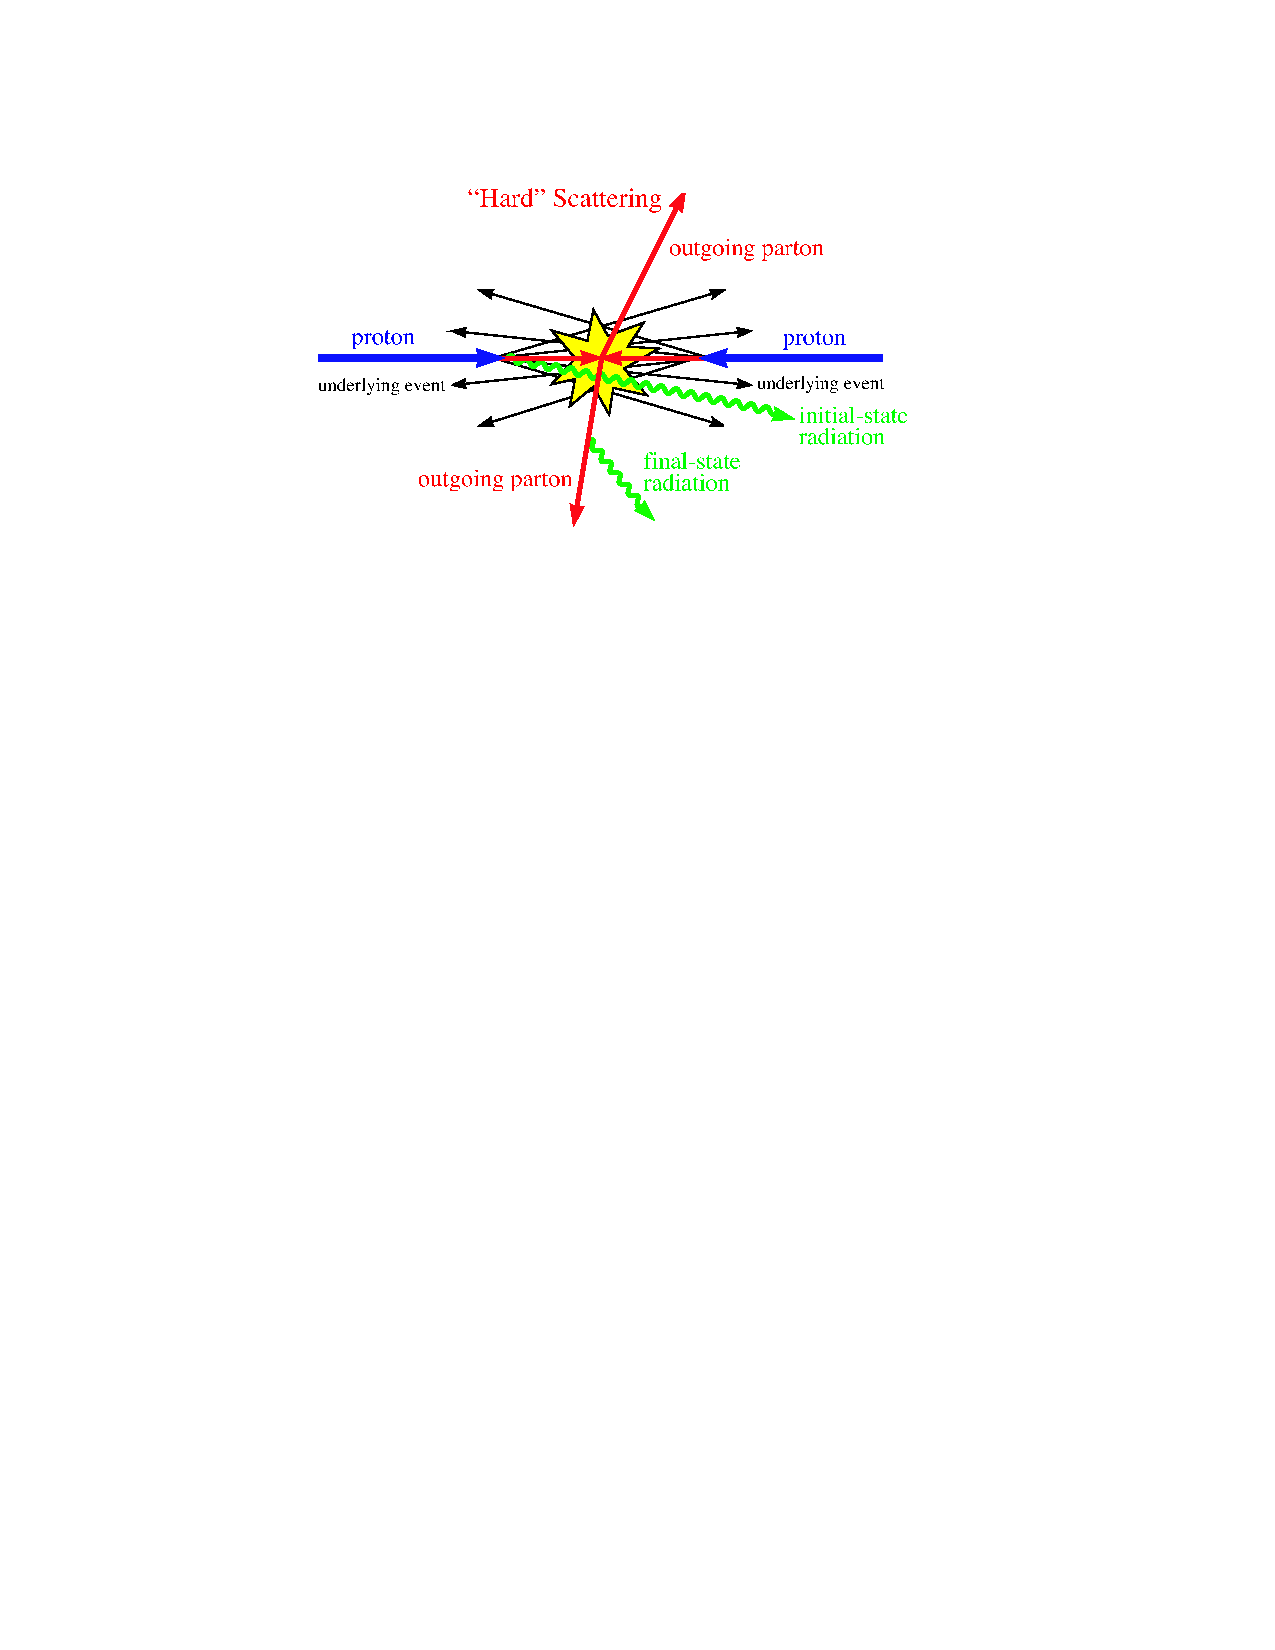
\includegraphics[width=0.47\textwidth]{pp_event}
    }
    \caption{\small
Sketch of a proton-proton collision. Figure from~\cite{Campbell:2006wx}.
}
    \label{fig:pp-event}
\end{figure}

\section{Monte-Carlo Simulation}
\label{sec:Theory-MC}

Simulated events are a crucial ingredient to a particle physics
measurement for a number of reasons. It is of course important to be able to
compare experimentally measured quantities such as \cx s and kinematic
distributions with predictions from the theory. Furthermore, simulated data
samples are important for calibrating the detector response and for estimating
selection efficiencies in order to translate from observed events
to a physical quantity such as a \cx. 

Simulated events are obtained by
means of \mc\ simulations, which use numerical integration to calculate matrix
elements and generate events. Generating events suitable for the purposes
outlined in the last paragraph typically consists of four steps:
calculation of the matrix element for the hard scattering, adding additional and
final state radiation using a parton shower,
simulating the hadronisation and finally embedding in the underlying event. These steps are described
in more details below. 

The calculation of the matrix element (ME) is
made at a fixed order in perturbative QFT, where the expansion is in terms of
the strong coupling constant \alphaS. The event generators used in this thesis
are either \intro{Leading Order (LO)}, where only the simplest diagrams
contributing to a process are calculated, or \intro{Next to Leading Order (NLO)},
where contributions from one loop diagrams are included. 

Both the incoming and any outgoing partons will emit soft collinear radiation in the form of other quarks and gluons. This is
modelled by the parton shower (PS), which models successive splittings of the
incoming or outgoing partons. In the case of outgoing partons they are radiated
until they reach an energy of $\sim 1$ \gev, at
which point the predictions of perturbative QCD become invalid and the partons
hadronise. For the incoming partons, the
shower is run in reverse to model the evolution of the parton back from its state
at the point of the hard scatter through splittings occurring within the proton,
with progressively lower energy until a cutoff scale of $\sim 1$ \gev\ is reached.

The process of hadronisation is not well described theoretically,
but relies on a number of phenomenological models. A common set of models are
the \intro{string models}, in which the
force between two coloured charges is modelled as an elastic string with
rising tension as the particles separate. If the string is stretched too far
it will snap, creating a new pair of colour charges. If a pair of opposite
colour charges are found close to each other, they are combined into a hadron.

Modern \mc\ integrators can calculate exact matrix elements with additional
partons from FSR in the matrix element. Whilst this increases the accuracy of
the \cx\ and kinematic distributions, it becomes necessary to `match' the
ME calculation to the PS, to ensure no double counting (since otherwise a
$2\ra3$ event could either come from a $2\ra3$ matrix-element event or a $2\ra2$
matrix element event with an additional parton coming from a splitting in the
parton shower. Different generators use different models for the parton
shower, hadronisation, and the ME-PS matching.

\subsection{\mc\ generators}
\label{sec:Theory-MC-gen}

A wide range of \mc\ integrators and event generators are available to simulate
processes of interest at the LHC. The
following generators are used in this thesis. For each generator, an outline of
how it is used and its general properties is given.

\begin{itemize}
    \item \mcfm ~\cite{Campbell:2011} is designed to calculate \cx s for
    femtobarn-level processes at hadron colliders. Matrix elements are
    calculated at NLO, incorporating full spin correlations. \mcfm\ is a \cx\
    calculator only and cannot produce unweighted events suitable for use in a
    physics analysis. Nevertheless it provides a useful toolkit for calculating
    \cx s, estimating the acceptance of the fiducial volume and studying the
    associated uncertainties due to \partDF\ and scale uncertainties.

    \item \powhegbox~\cite{Alioli:2010xd} is a general framework for implementing
    NLO calculations. It uses the \powheg\ method to match the NLO matrix
    elements to the parton shower. \powhegbox\ must be interfaced to an external
    program for the implementation of the parton shower - in this thesis
    \powhegbox\ is interfaced to \pythia for showering. Specific details of the
    implementation of the \ZZ\ process in \powhegbox\ is given
    in~\cite{Melia:2011tj}; the \ggZZ\ process is not included. 
    Samples generated using \powhegbox\ are used as the main signal samples for
    the \qqZZ\ process, used to optimise the selection, estimate selection
    acceptances and systematics and compare observed distributions with theory.

    \item \ggtwoZZ~\cite{gg2ZZ} is a specialist generator used to simulate the
    \ggZZ\ process. Events generated with \ggtwoZZ\ are used in conjunction with
    the \powhegbox\ events as the main signal sample. It is interfaced to the
    \herwig\ to provide the parton shower and \jimmy~\cite{bib:jimmy} to model the underlying
    event. Its sister generator, \ggtwoWW, is used to simulate the background
    from \ggWW~\cite{Binoth:2006mf}.

    \item \sherpa~\cite{Gleisberg:2008ta} is a LO generator, capable of
    simulating the \qqZZ\ process with up to three additional hard partons in the matrix element. It
    uses an extended version of the CKKW scheme~\cite{Hoeche:2009rj} to match to the matrix element to the parton shower,
    and provides its own simulation of the parton shower, QED radiation and
    the underlying event. \sherpa\ is also capable of simulating aTGCs. It is
    used as a cross-check to \powhegbox\ and to estimate the impact
    of uncertainties
    arising from different implementations of the parton shower and QED
    radiation. It is also used to simulate aTGC samples.
    Version 1.3.1 is used to simulate \qqZZllll\ at 7 \tev, and 1.4.0 is used at
    8 \tev.

    \item \pythia is a LO generator which uses a library of $2\ra2$
    matrix elements covering almost all \sm\ processes to model the signal
    process and a \pt\ ordered parton shower to model additional radiation.
    The Fortran77 based
    \pythia6~\cite{pythia} is used at 7 \tev\, whilst the C++ based
    \pythia8~\cite{Sjostrand:2007gs} is used at 8 \tev. \pythia is used to
    provide showering for many of the other generators described here, and is
    also used as a cross-check to the main signal samples.

    \item \herwig~\cite{Herwig} is another general purpose LO generator, generating events in a
    similar way is used to \pythia, but using an angular-ordered parton shower.
    %and cluster model for hadronisation.
    It is used for generating inclusive samples (all final
    states) of $WW$ and $WZ$ production, used in estimating background from
    other diboson processes.

    \item \herwigPP~\cite{Bahr:2008pv} is a C++ based generator based on the
    Fortran \herwig. It includes NLO calculations of a number of processes
    using the \powheg\ matching scheme. \herwigPP\ is only used for comparison
    of \ZZ\ event kinematics at generator level.

    \item \mcatnlo~\cite{bib:mcatnlo} is a NLO generator, and was the first
    generator to implement NLO ME to PS matching, using the so-called \mcatnlo\
    technique. \mcatnlo\ is used to simulate the background processes \ttbar,
    \Wt\ and single-top at 7 \tev. \mcatnlo\ can simulate \qqZZ, but only in the
    zero-width approximation where the lineshape of the \Z\ boson is not
    included. For this reason \mcatnlo\ is not used for signal simulation,
    though the generator level predictions of \mcatnlo\ are compared to other
    generators in the following section.

    \item \alpgen~\cite{alpgen} is a LO genertor for simulating multi-parton
    processes in hadron interactions. It can simulate $W$ and \Z\ production
    with up to 6 additional partons in the matrix element. It is interfaced to
    \herwig\ for the parton shower, using the MLM matching
    scheme~\cite{Mangano2002343}. It is used to simulate \W\ and \Z\ bosons in
    association with jets, as well as low mass Drell-Yan and \Wg and \Zg.

    %\item \pythiaB is used to simulate events with heavy favour dijets. Since
    %these are of interest as background processes to events with leptons, a
    %dilepton filter is applied at generator level, requiring two $e$ or $\mu$ with
    %\ptgt{10}.

    %\item \madgraph~\cite{madgraph} \Wg\ and \Zg (7 tev).

\end{itemize}



\graphicspath{{Chapters/TheoryZZProduction/Figures/}}
\chapter{ZZ Production}
\label{chap:TheoryZZProduction}

\section{Introduction}

Production of pairs of \Z\ bosons, so called \intro{diboson \ZZ\ production} is a
rare process at particle colliders, but has a very striking signature
and low backgrounds. The study of diboson \ZZ\ production is of great interest
as it provides a precision test of the \sm, and unique opportunity to
probe the structure of the electroweak sector. 
The $ZZZ$ and $ZZ\gamma$ neutral triple gauge boson
couplings (nTGCs) are zero in the Standard Model, but are predicted to exist at the
level of $10^{-4}$ to $10^{-3}$ in certain new-physics
models~\cite{Ellison:1998}. Non-resonant \ZZ\ production is also the
irreducible background to \HZZ\ decays, one of key channels in Higgs boson physics
at the LHC. The CMS~\cite{CMS_Higgs:2012gu} and ATLAS~\cite{ATLAS_Higgs:2012gk}
experiments both recently reported the discovery of a new boson with mass near
125 \gev\ in the search for the Higgs boson. \HZZ\ decays were a key
search channel for this discovery, contributing a local significance of 3.6
$\sigma$ to the overall local significance of 6.0 $\sigma$ (the other
contributing channels were \Hgg\ and \HWW). Understanding non-resonant \ZZ\
production was essential for such a discovery, and continues to be important for
studying the properties of the new boson.

\section{\ZZ\ production at hadron colliders}

At hadron colliders, \qqZZ\ proceeds at tree level via $t$- and $u$-channel
quark-antiquark annihilation as shown in~\fig{theoryzz-fd-qqZZ}. Since \ZZZ\ and
\ZZg\ couplings are forbidden in the \sm\ there is no contribution from
$s$-channel $q\bar{q}$ annihilation at tree level, although contributions from
fermion loops contribute at $\mathcal{O}(10^{-4})$~\cite{Gounaris:2000dn}.
Gluon-gluon fusion processes will also
contribute via quark box diagrams, as shown in~\fig{theoryzz-fd-ggZZ}. Although
these are NNLO and are suppressed by a factor of
$\alpha_s^2$, due to the high gluon content of the proton at LHC energies they
still contribute a sizeable fraction of the total \ZZ\ production \cx\,
contributing approximately 10\%~\cite{Campbell:2011} of the cross-section,
depending on the centre of mass energy and the definition of the \cx.
This is discussed in more detail below.

%% s- and u-channel feynman diagrams for qqZZ
\begin{figure}
\centering
    \subfigure{
        \begin{fmffile}{tchan}
        \begin{fmfgraph*}(36,20)
            \fmfleft{i1,i2}
        \fmfright{o1,o2}
        \fmflabel{$u,d$}{i2}
        \fmflabel{$\bar{u},\bar{d}$}{i1}
        \fmfright{o1,o2}
        \fmflabel{$Z/\gamma^{*}$}{o1}
        \fmflabel{$Z/\gamma^{*}$}{o2}
        \fmf{fermion}{i2,v2,v1,i1}
        %\fmf{fermion}{v2,i2}
        %\fmf{fermion}{v1,i1}
        \fmf{photon}{v1,o1}
        \fmf{photon}{v2,o2}
        % uncommment this line if you want dots at the vertices
            %\fmfdotn{v}{4}
        \end{fmfgraph*}
        \end{fmffile}
    }
    \hspace{10mm}
    \subfigure{
        \begin{fmffile}{tchan2}
        \begin{fmfgraph*}(36,20)
            \fmfleft{i1,i2}
        \fmfright{o1,o2}
        \fmflabel{$u,d$}{i2}
        \fmflabel{$\bar{u},\bar{d}$}{i1}
        \fmfright{o1,o2}
        \fmflabel{$Z/\gamma^{*}$}{o1}
        \fmflabel{$Z/\gamma^{*}$}{o2}
        \fmf{fermion}{i2,v2,v1,i1}
        %\fmf{fermion}{v2,i2}
        %\fmf{fermion}{v1,i1}
        \fmf{phantom}{v1,o1}
        \fmf{phantom}{v2,o2}
        \fmf{photon,tension=0}{v2,o1}
        \fmf{photon,tension=0}{v1,o2}
        % uncommment this line if you want dots at the vertices
            %\fmfdotn{v}{4}
        \end{fmfgraph*}
        \end{fmffile}
    }
        \vspace{8mm}
\caption{Leading order Feynman diagrams for \ZZ\ production in proton-proton
collisions. The left hand diagram shows $t$-channel \qqZZ, the right hand
diagram the equivalent $u$-channel process. The tree level $s$-channel process is forbidden
in the \sm.}
\label{fig:theoryzz-fd-qqZZ}
\end{figure}

%% gg diagrams
\begin{figure}
\centering
        \vspace{10mm}
    \subfigure{
        \begin{fmffile}{gluonbox}
        \begin{fmfgraph*}(36,20)
            \fmftop{i2,d2,o2}
            \fmfbottom{i1,d1,o1}
            \fmfleft{i1,i2}
        \fmflabel{$g$}{i1}
        \fmflabel{$g$}{i2}
        \fmfright{o1,o2}
        \fmflabel{$Z/\gamma^{*}$}{o1}
        \fmflabel{$Z/\gamma^{*}$}{o2}
        \fmf{gluon}{i1,v1} %incoming gluon
            \fmf{fermion}{v1,v3} % + bottom of box --> correct
            \fmf{photon}{v3,o1}
        \fmf{photon}{v4,o2}
        \fmf{fermion}{v4,v2}% + top of box --> correct
            \fmf{gluon}{v2,i2}
        \fmf{fermion,tension=0}{v2,v1}% + left hand side of box correct
            \fmf{fermion,tension=0}{v3,v4} % + right hand side of box
            % uncommment this line if you want dots at the vertices
            %\fmfdotn{v}{4}
        \end{fmfgraph*}
        \end{fmffile}
    }
    \hspace{2mm}
    \subfigure{
        \begin{fmffile}{gluonbox2}
        \begin{fmfgraph*}(36,20)
          % A homage to T. Barber????
          \fmfcmd{%
    style_def tomion expr p =
    cdraw p;
    cfill (harrow (p, .5))
    enddef;}
            \fmfleft{i1,i2}
        \fmflabel{$g$}{i1}
        \fmflabel{$g$}{i2}
        \fmfright{o1,o2}
        \fmflabel{$Z/\gamma^{*}$}{o1}
        \fmflabel{$Z/\gamma^{*}$}{o2}
        \fmf{gluon}{i1,v1} %incoming gluon
            \fmf{fermion}{v3,v1}% + bottom of box --> correct
            \fmf{photon}{v3,o1}
        \fmf{photon}{v4,o2}
        \fmf{fermion}{v4,v2}% + top of box --> correct
            \fmf{gluon}{v2,i2}
        \fmf{tomion,tension=0}{v2,v3}% Diagonal Top L to bottom R
            \fmf{tomion,tension=0}{v1,v4} %Diaganol Bottom L to top R 
            % uncommment this line if you want dots at the vertices
            %\fmfdotn{v}{4}
        \end{fmfgraph*}
        \end{fmffile}
    }
    \hspace{2mm}
    \subfigure{
        \begin{fmffile}{gluonbox3}
        \begin{fmfgraph*}(36,20)
            \fmfleft{i1,i2}
        \fmflabel{$g$}{i1}
        \fmflabel{$g$}{i2}
        \fmfright{o1,o2}
        \fmflabel{$Z/\gamma^{*}$}{o1}
        \fmflabel{$Z/\gamma^{*}$}{o2}
        % Incoming gluons
        \fmf{gluon}{i1,v1} 
        \fmf{gluon}{v2,i2}
        % Box
        \fmf{fermion}{v1,v3}% + bottom of box --> correct
        \fmf{fermion}{v4,v2}% + top of box --> correct
        \fmf{fermion,tension=0}{v2,v1}% + left hand side of box correct
        \fmf{fermion,tension=0}{v3,v4} % + right hand side of box
        %Outging Z
        \fmf{photon,tension=0}{v3,o2}
        \fmf{photon,tension=0}{v4,o1}
        \fmf{phantom}{v3,o1}
        \fmf{phantom}{v4,o2}
            % uncommment this line if you want dots at the vertices
            %\fmfdotn{v}{4}
        \end{fmfgraph*}
        \end{fmffile}
    }
        \vspace{8mm}
\caption{Feynman diagrams for \ggZZ. Although these are NNLO processes and thus
supressed by a factor of $\alpha_s^{2}$ they still make a significant
contribution at LHC energies due to the high gluon content of the proton}
\label{fig:theoryzz-fd-ggZZ}
\end{figure}

\subsection{\ZZ\ Decay Modes}

\Z\ bosons can decay to a quark-antiquark pair, a neutrino-antineturino pair or
a pair of oppositely charged leptons. The branching fractions to each of the
final states are well known~\cite{PDG}, and are 69.9\% for $q \bar{q}$, 20.0\%
for $\nu\bar{\nu}$ and 10.1\% for \ll. In \ZZ\ decays, each boson decays
independantly, so the branching fraction for a given final state is the product
of the branching fractions for the two \Z\ bosons. The measurements in this
thesis are all based on measurements of \ZZllll, where $\ell = e,\mu$, giving
three final states \eeee, \mmmm\ and \eemm. The
branching fractions to these final states are as follows:

\begin{align}
\mathcal{B}(\ZZeeee) = 0.113 \errSym{0.008}\,\% \\
\mathcal{B}(\ZZmmmm) = 0.113 \errSym{0.014}\,\% \\
\mathcal{B}(\ZZeemm) = 0.226 \errSym{0.016}\,\% 
\end{align}

\subsection{Cross Section Definition}

The \cx\ for non-resonant \ZZ\ production can be defined in a number of
ways. One definition is to use a zero-width approximation for the \Z\ bosons and
calculate a total \cx. Alternatively, the natural width of the \Z\
bosons can be used, and requirements made on the invarient masses of the \Z\
bosons to define a \cx. In this thesis, measurements of two total \ZZ\ \cx s
are presented: an \intro{on-shell} \cx\, assuming natural width for the
\Z\ bosons and requiring both bosons have mass in the range \sstooosZ, and a
\cx\ allowing one of the \Z\ bosons to be off shell with $m_{\Z}>20$
\gev.

Measurements are also presented in a restricted phase space, termed a
\intro{fiducial volume}, which corresponds closely to the experimental selection
requirements described in~\chap{ObjEventSelection}. The corresponding
\intro{fiducial \cx} has smaller theoretical uncertanties than the total \cx,
where uncertainties on the extrapolation from the experimentally measured
fiducial \cx\ to the total \cx\ arise due to uncertainties on the \partDF\ and
the factorisation and renormalisation scales. The fiducial volumes used for the
7 \tev\ and the 8 \tev\ measurements are slightly different, reflecting the
different experimental selections. They are defined below. The fiducial
cross-sections are measured using decays where both \Z\ bosons decay to either electrons
or muons. The fiducial
cross-sections are then extrapolated to the total cross-section correcting for
the geometric acceptance of the fiducial volume and the branching
fractions to leptons.

\subsubsection{7 \tev\ Fiducial Cross Section Definitions}

The \zzllll\ on-shell (\ZZ) fiducial \cx\ is defined as:

\begin{itemize}
\item{\ZorgZorglplmlplm, $\ell = e,\mu$}
\item{ $66 < m_{12}(\Zorgv) <  116\GeV$, where $m_{12}(\Zorgv)$ is
the mass of the \Z\ reconstructed from the first and second leptons.  The
lepton pairings are assigned by choosing the set of 
same-flavor, opposite-sign lepton pairs that minimises the sum of distances from
the PDG~\cite{PDG} value of the \Z\ mass:
\begin{equation}
|m_{1,2}(\Zorgv) - \mZPDG| + |m_{3,4}(\Zorgv) - \mZPDG|
\end{equation}
}
\item{ $66 < m_{34}(\Z/\gamma^*) <  116\GeV$, where $m_{34}(\Z/\gamma^*)$ is
the mass of the \Z\ reconstructed from the third and fourth leptons;}
\item All four leptons have transverse momentum satisfying $\pT^{\ell} > 7\GeV$;
\item All four leptons have pseudo-rapidity satisfying $|\eta^{\ell}| < 3.16$.
\item{ The minimum distance between any two leptons in the event must satisfy
$\mathrm{min}(\dR(\ell,\ell)) > 0.2$, where $\dR = \sqrt{\Delta \phi^{2} +
\Delta \eta^{2}}$.}
\end{itemize}

The \zzllll\ fiducial cross-section, allowing one \Z\ to be off-shell ($ZZ^*$), is defined as:

\begin{itemize}
\item $(\Z/\gamma^*)(\Z/\gamma^*)\rightarrow\ll\ll$, $\ell = e,\mu$;
\item $66 < m_{12}(\Z/\gamma^*) <  116\GeV$;
\item $m_{34}(\Z/\gamma^*) > 20\GeV$;
\item $\pT^{\ell} > 7\GeV$;
\item $|\eta^{\ell}| < 3.16$.
\item $\mathrm{min}(|\Delta R(\ell,\ell)|) > 0.2$.
\end{itemize}

In this case the tighter mass cut is applied to the pair closest to the PDG \Z\
boson mass.

\subsubsection{8 \tev\ Fiducial Cross Section Definitions}

tbc

\subsection{Cross Section}

~\tab{cx-eemm-mcfm} shows cross sections for the \ZZeemm\ process at 7 \tev\ and
at 8 \tev, calculated using version 6.3 of the
\mcfm\cite{Campbell:2011} program. The cross-section in the zero-width approximation is shown, as
well as the cross sections allowing for the natural width of the \Z\ boson and
applying mass cuts.  The cross-sections after applying the requirements defining
the fiducial volume are also shown. 
In all cases, the CT10~\cite{CT10} \partDF\ set is used, and the factorisation and renormalisation scales are set
to $\mu_{R} = \mu_{F} = \mZZ/2$. The error due to the \partDF\ uncertainty is
evaluated by using the 52 CT10 error sets, and the error due to the choice of
\fact\ and \renorm\ scales is evaluated by varying them
simultaneously up and down by a factor of two. 

The percentage contributions from
gluon-gluon fusion processes are shown in~\fig{}.

Total cross sections are shown in~\tab{cx-total-mcfm}. These are also
calculated using the \mcfm\ program, with the settings as described above, by
calculating the cross-section for \ZZeemm\ then correcting for the branching
fraction $\mathcal{B}(\ZZeemm)$. 

\begin{align}
\sigma^{\rm tot,SM}_{ZZ} = 5.9\ \pm 0.2\ {\rm
(theory)\
pb} \\
\sigma^{\rm tot,SM}_{ZZ} = 7.4\ \pm 0.4\ {\rm (theory)\ pb} \\
\sigma^{\rm fid,SM}_{\ZZllll} = 19.0\ ^{+1.1}_{-1.0}\ {\rm (theory)\ fb} 
\end{align}

\begin{table}[htbp]
\small
\begin{center}
\begin{tabular}{lcccccc} \hline\hline
          & \multicolumn{3}{c}{$\sqrt{s} = 7$ \tev} &
          \multicolumn{3}{c}{$\sqrt{s} = 8$ \tev} \\
          & \multicolumn{1}{c}{$\sigma(ee\mu\mu)$~(fb)} &\multicolumn{2}{c}{Value shift (\%)}  & \multicolumn{1}{c}{$\sigma(ee\mu\mu)$~(fb)} &\multicolumn{2}{c}{Value shift (\%)}\\
          &            & \partDF       & Scale  &            & \partDF       & Scale  \\
\hline
Zero-width  & \TheoryCxSevenZeroWidth & \TheoryCxSevenZeroWidthCTerrPerc &
\TheoryCxSevenZeroWidthScaleErrPerc &\TheoryCxEightZeroWidth &
\TheoryCxEightZeroWidthCTerrPerc & \TheoryCxEightZeroWidthScaleErrPerc \\
\hline
$66<m_{12}<116$~GeV   & \TheoryCxSevenOnShell & \TheoryCxSevenOnShellCTerrPerc &
\TheoryCxSevenOnShellScaleErrPerc &\TheoryCxEightOnShell &
\TheoryCxEightOnShellCTerrPerc & \TheoryCxEightOnShellScaleErrPerc \\

$66<m_{34}<116$~GeV  &&&& \\

\hline
$66<m_{12}<116$~GeV   & \TheoryCxSevenOnShellFid & \TheoryCxSevenOnShellFidCTerrPerc &
\TheoryCxSevenOnShellFidScaleErrPerc &\TheoryCxEightOnShellFid &
\TheoryCxEightOnShellFidCTerrPerc & \TheoryCxEightOnShellFidScaleErrPerc \\
$66<m_{34}<116$~GeV   &&&& \\
$\pT(\ell)>7$~GeV,  &&&& \\
$|\eta(\ell)|<3.16$, $\dR<0.2$ &&&& \\
\hline        
$66<m_{12}<116$~GeV   & \TheoryCxSevenOffShell & \TheoryCxSevenOffShellCTerrPerc &
\TheoryCxSevenOffShellScaleErrPerc &\TheoryCxEightOffShell &
\TheoryCxEightOffShellCTerrPerc & \TheoryCxEightOffShellScaleErrPerc \\
$m_{34}>20$~GeV       &&&& \\
\hline
$66<m_{12}<116$~GeV   &  \TheoryCxSevenOffShellFid & \TheoryCxSevenOffShellFidCTerrPerc &
\TheoryCxSevenOffShellFidScaleErrPerc &\TheoryCxEightOffShellFid &
\TheoryCxEightOffShellFidCTerrPerc & \TheoryCxEightOffShellFidScaleErrPerc \\
$m_{34}>20$~GeV       &&&& \\
$\pT(\ell)>7$~GeV, &&&& \\
$|\eta(\ell)|<3.16$, $\dR<0.2$  &&&& \\
\hline\hline
\end{tabular}
\end{center}
\caption{Cross sections and acceptance calculated at NLO in QCD with MCFM version 6.1. The 
         central values are calculated using both the MSTW2008 and CTEQ6.6 PDF set; the errors 
         shown are from Monte Carlo statistics. The cross sections shown are for the $ee\mu\mu$ final 
         state, and should be multiplied by two to give the value corresponding to the $4\ell$ final state. The column labeled 
	 ``CTEQ6.6 error set" gives the error derived from the 44 CTEQ6.6 error sets, while 
         the one labeled `Scale' gives the error from changing the factorisation and renormalisation 
         scales up and down by a factor of two from the default value of \mZ. The acceptance,
         $A_{ZZ}$, is the ratio of the cross section in $66<m_{12}<116$~GeV, $66<m_{34}<116$~GeV,
         $\pT(\ell)>7$~GeV, $\eta(\ell)|<2.7$ to the on-shell cross section.}
\label{table:cx-eemm-mcfm}
\end{table} 

\section{Monte-Carlo Simulation}

\subsection{Signal Process Simulation}

\subsection{Background Process Simulation}

\subsection{Comparison of \ZZllll\ at 7 \tev\ and 8 \tev}

Figures~\ref{fig:gen-comp-7-8-ZZ} and ~\ref{fig:gen-comp-7-8-ZZs} show comparisons of the kinematic distributions in \ZZllll\
decays at 7 \tev\ and 8 \tev, simulated using the \powhegbox\cite{Melia:2011tj} generator
to model the quark-anitquark annihilation process and the \ggtwoZZ\cite{gg2ZZ} genrator to
model the gluon-gluon fusion process. 
%In both cases the CT10~\cite{CT10}
%\partDF\ set is used, and the factorisation and renormalisation scales are set
%to $\mu_{R} = \mu_{F} = \mZZ$. 
In~\fig{gen-comp-7-8-ZZ} the kinematic
distributions are plotted after requiring that both \Z\ bosons have \sstooos,
whilst in~\fig{gen-comp-7-8-ZZs} the requirement on the most off-shell \Z\ is
relaxed to \mZgtt. In both cases the distributions of \mZZ, \ptZZ, leading \Z\
\pt\ and the \pt\ of the highest and lowest \pt\ lepton are observed to tend towards
slightly higher energies at 8 \tev\ than at 7 \tev. The pseudo-rapidity
distributions of the highest and lowest \pt\ leptons are observed to be wider at
8 \tev, with a greater fraction of the leptons being at high pseudo-rapidity.

\begin{figure}
\centering
        \vspace{-5mm}
    \subfigure[]{
        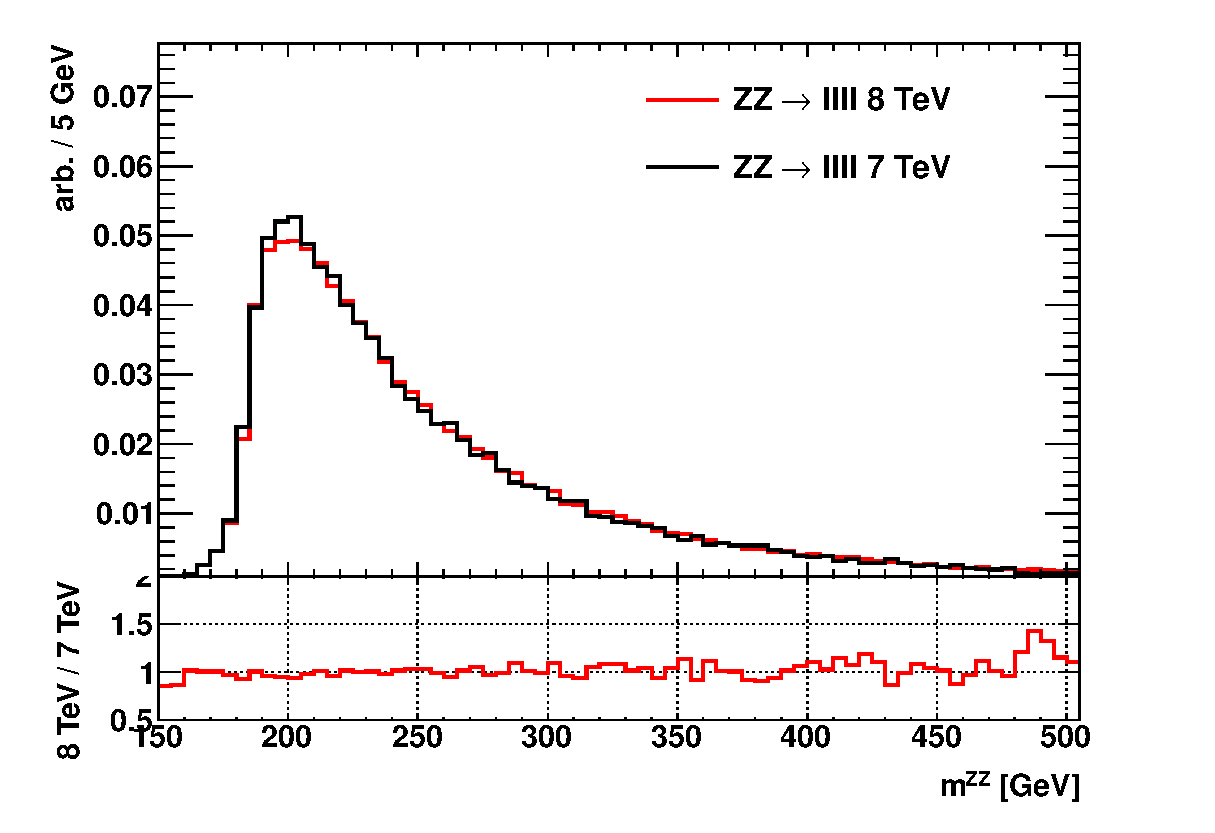
\includegraphics[width=0.47\textwidth]{Compare20112012/truth_ZZ_ZZ_m_lin}
    }
    \subfigure[]{
        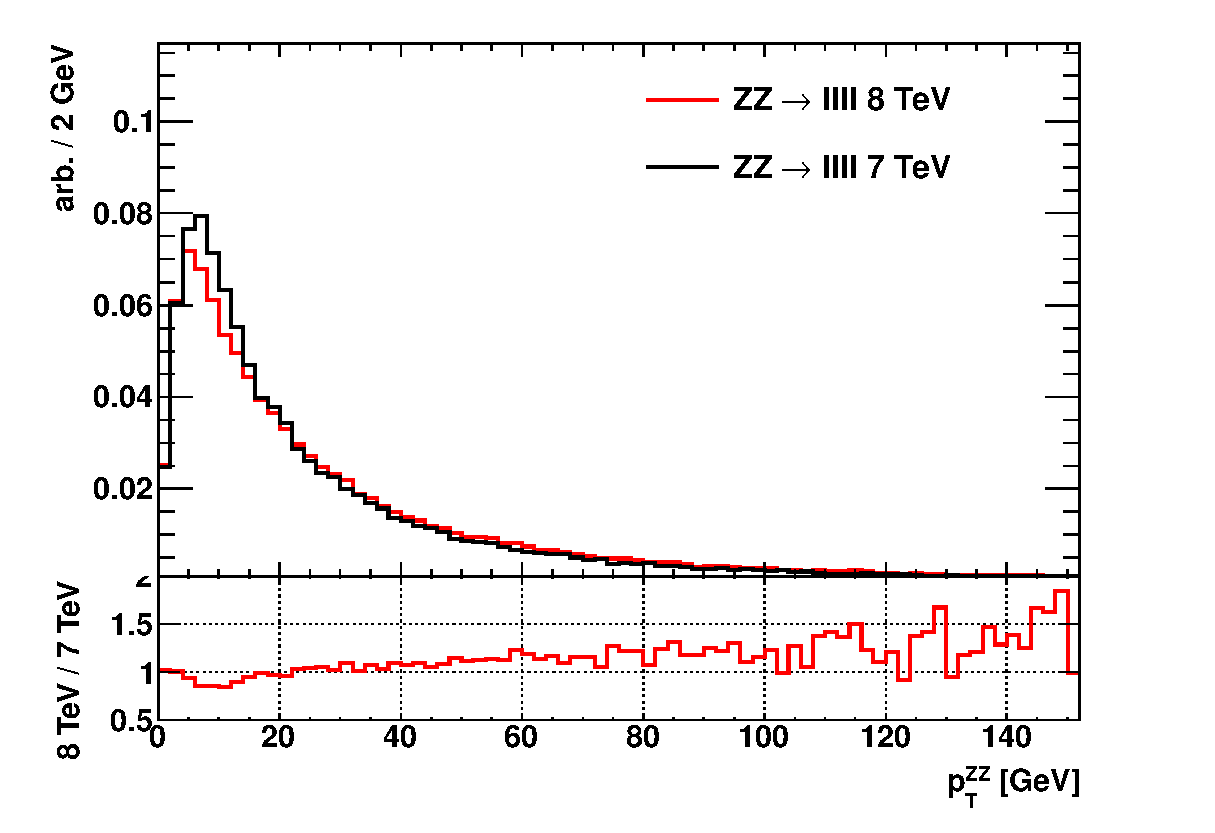
\includegraphics[width=0.47\textwidth]{Compare20112012/truth_ZZ_ZZ_pt_lin}
    }
        \vspace{-2mm}
    \subfigure[]{
        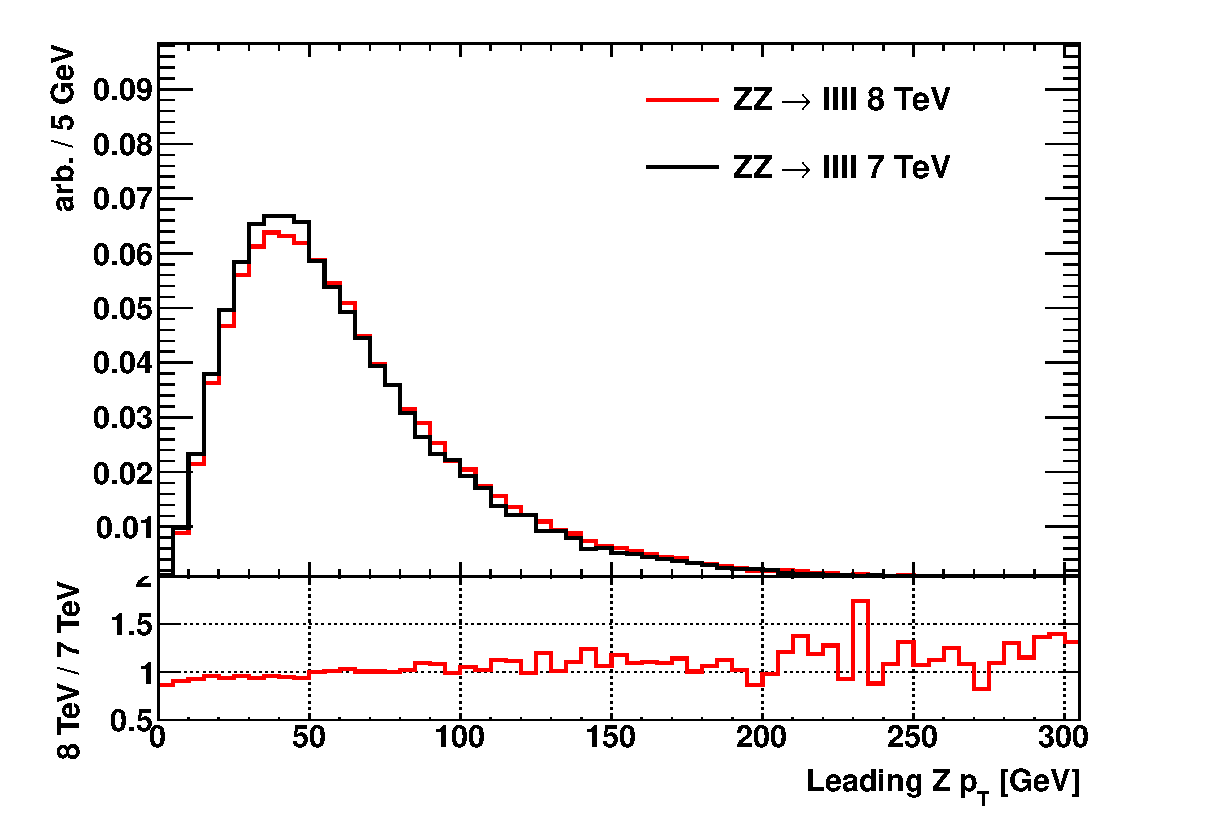
\includegraphics[width=0.47\textwidth]{Compare20112012/truth_ZZ_Z1_pt_lin}
    }
    \subfigure[]{
        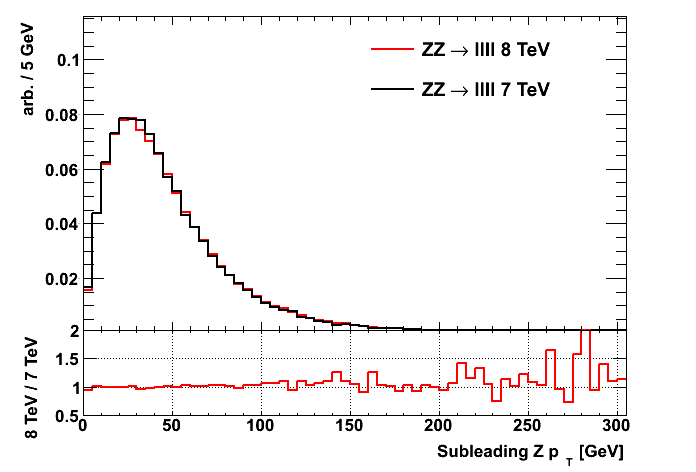
\includegraphics[width=0.47\textwidth]{Compare20112012/truth_ZZ_Z2_pt_lin}
    }
        \vspace{-2mm}
    \subfigure[]{
        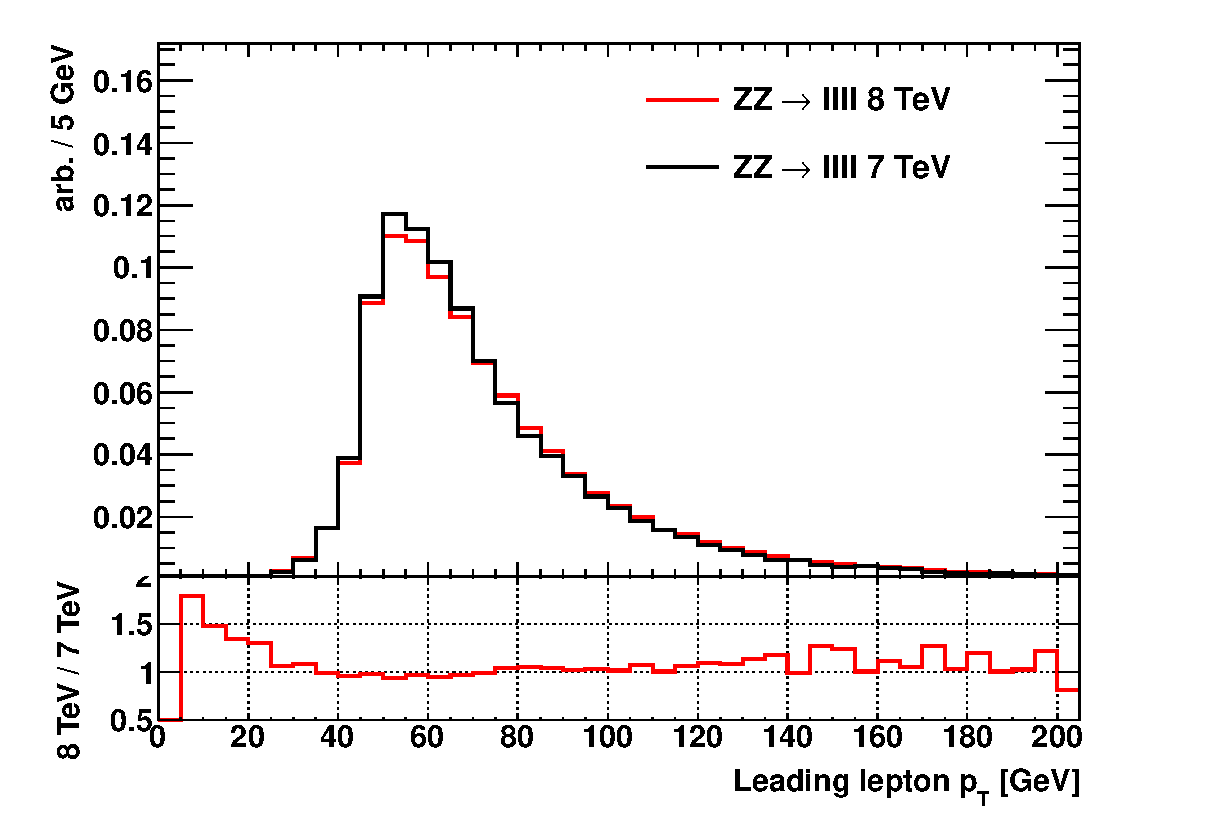
\includegraphics[width=0.47\textwidth]{Compare20112012/truth_ZZ_lep_1_pt_lin}
    }
    \subfigure[]{
        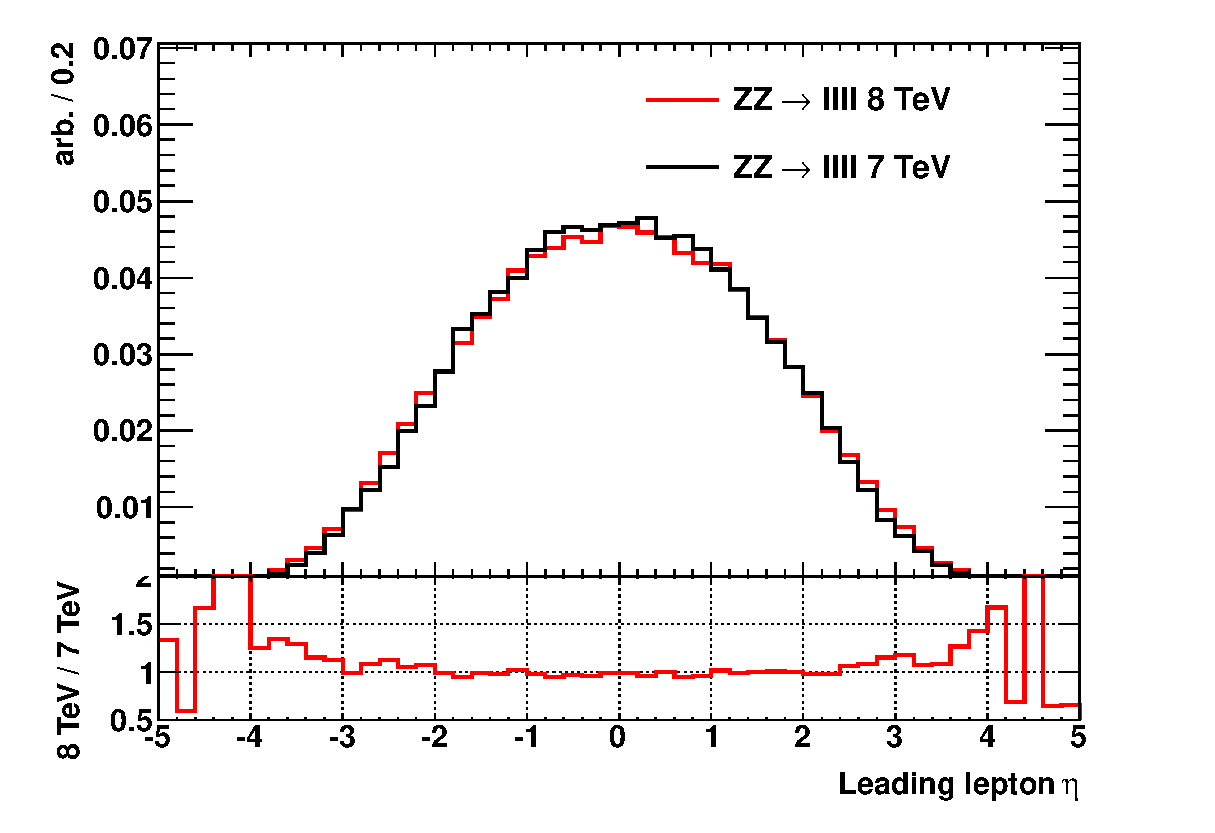
\includegraphics[width=0.47\textwidth]{Compare20112012/truth_ZZ_lep_1_eta_lin}
    }
        \vspace{-2mm}
    \subfigure[]{
        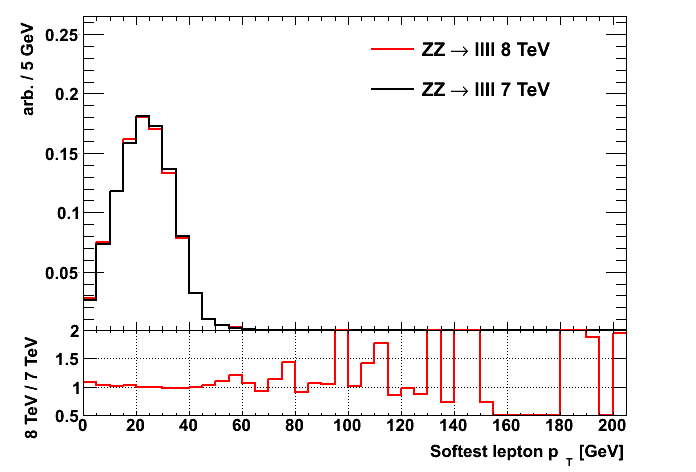
\includegraphics[width=0.47\textwidth]{Compare20112012/truth_ZZ_lep_4_pt_lin}
    }
    \subfigure[]{
        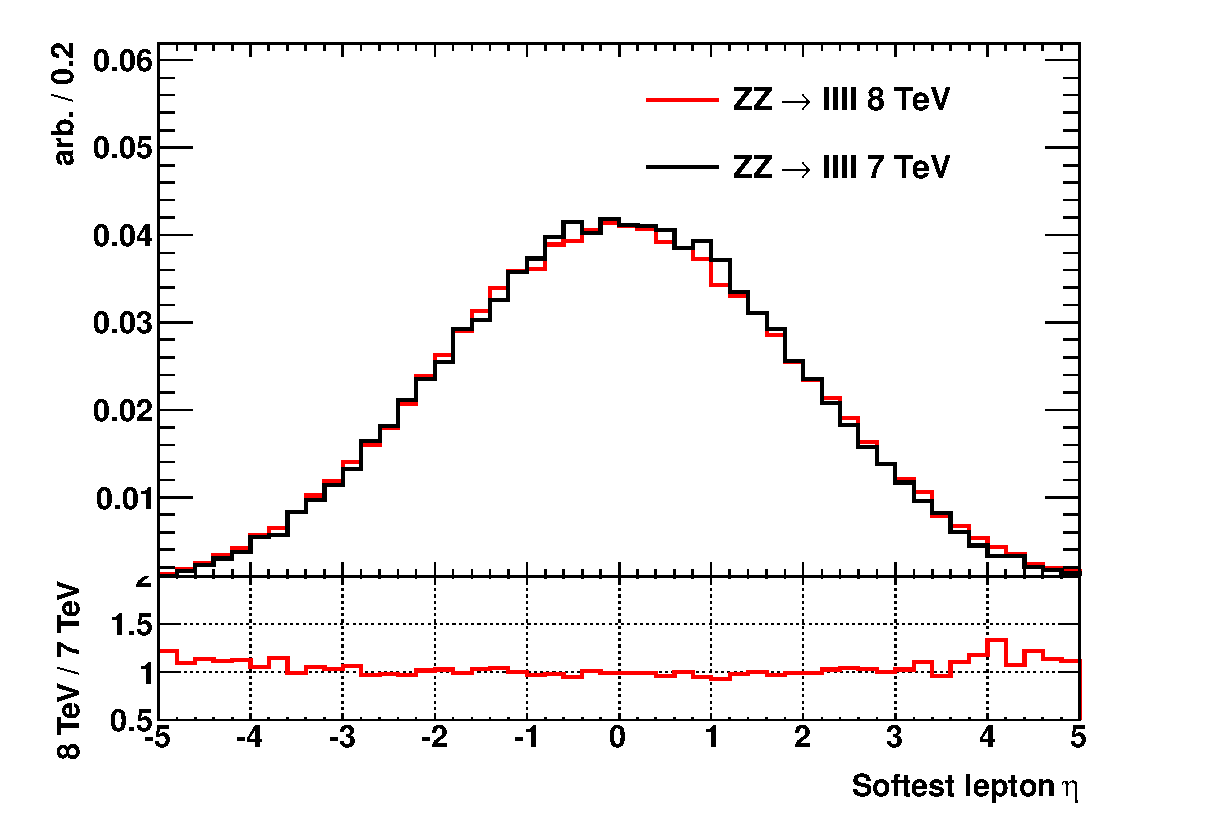
\includegraphics[width=0.47\textwidth]{Compare20112012/truth_ZZ_lep_4_eta_lin}
    }
        \vspace{-2mm}
    \caption{\small Comparison of generator level distribtuions, normalised to
    unit area, for \ZZllll\ for 7
    \tev\ and 8 \tev. Both \Z\ bosons are required to have \sstooosZ. Figures (a)
    and (b) show the mass and \pt\ of the \ZZ\ system,
    respectively. Figures (c) and (d) show the \pt\ of the
    leading and subleading \Z, respectively. Figure (e) shows the \pt\ of the highest \pt\ lepton in the event, and figure (f) shows its
   $\eta$. Similarly figures (g) and (h) show the \pt\ and $\eta$ of the lowest
   \pt\ lepton in the event.}
    \label{fig:gen-comp-7-8-ZZ}
\end{figure}

\begin{figure}
\centering
        \vspace{-5mm}
    \subfigure[]{
        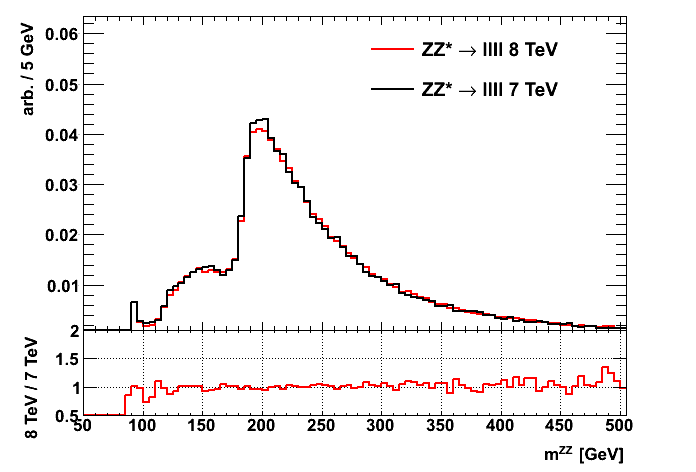
\includegraphics[width=0.47\textwidth]{Compare20112012/truth_ZZs_ZZ_m_lin}
    }
    \subfigure[]{
        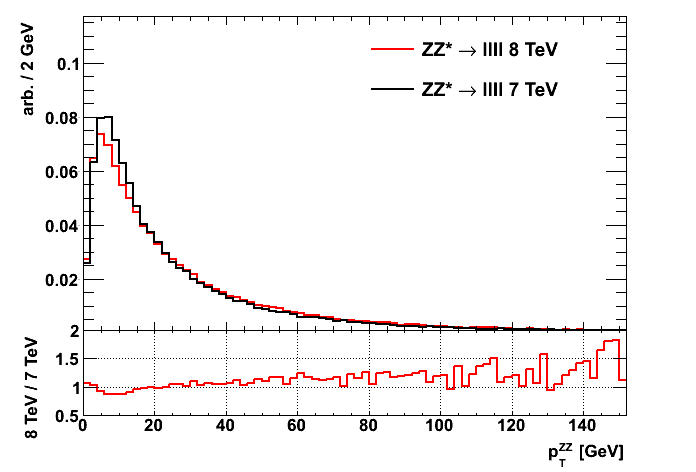
\includegraphics[width=0.47\textwidth]{Compare20112012/truth_ZZs_ZZ_pt_lin}
    }
        \vspace{-2mm}
    \subfigure[]{
        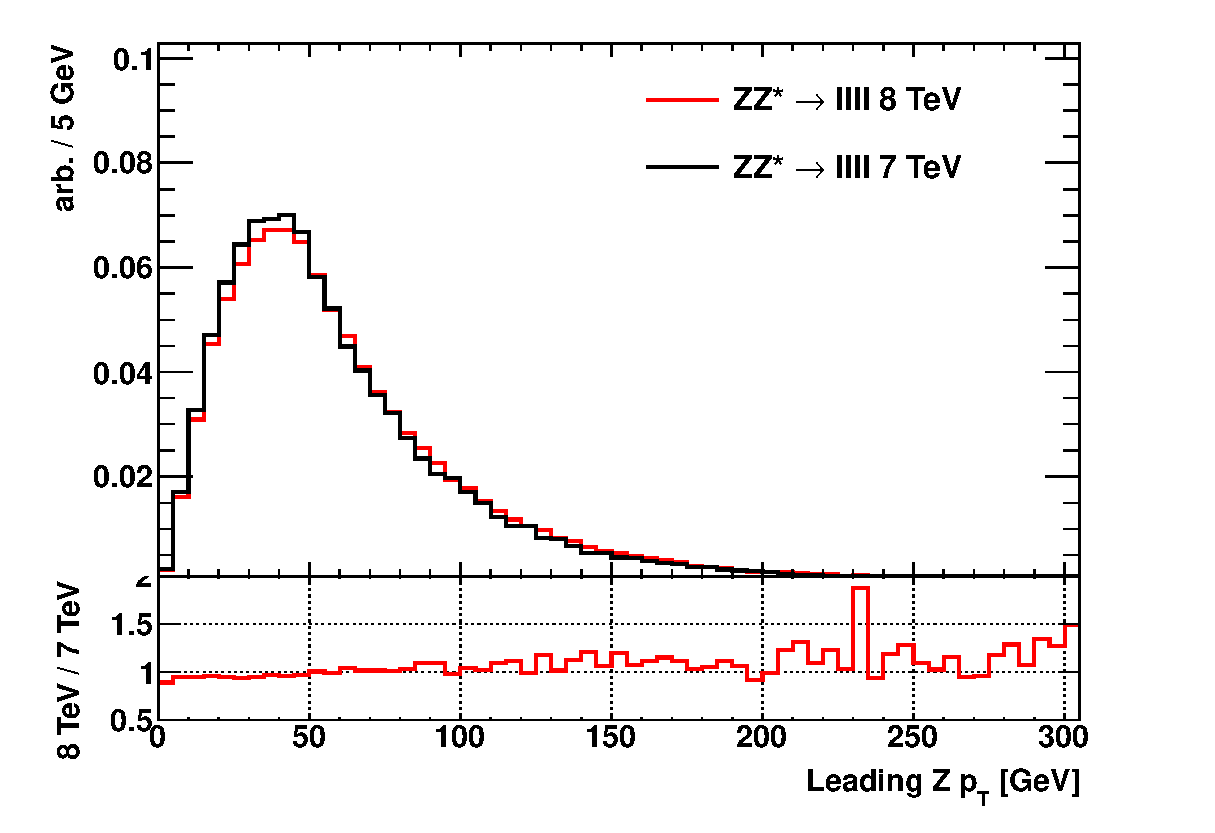
\includegraphics[width=0.47\textwidth]{Compare20112012/truth_ZZs_Z1_pt_lin}
    }
    \subfigure[]{
        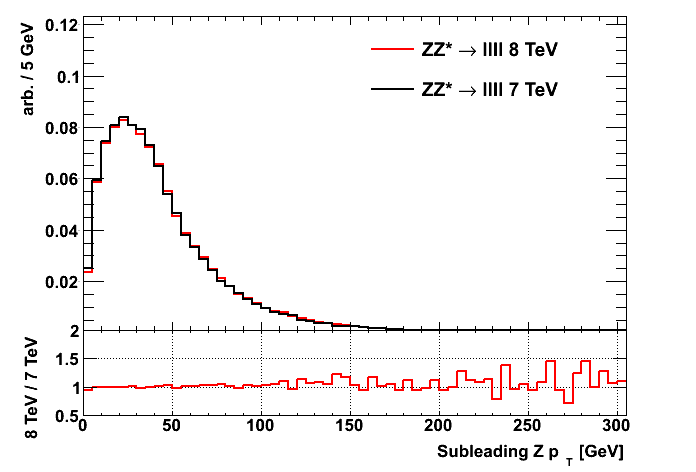
\includegraphics[width=0.47\textwidth]{Compare20112012/truth_ZZs_Z2_pt_lin}
    }
        \vspace{-2mm}
    \subfigure[]{
        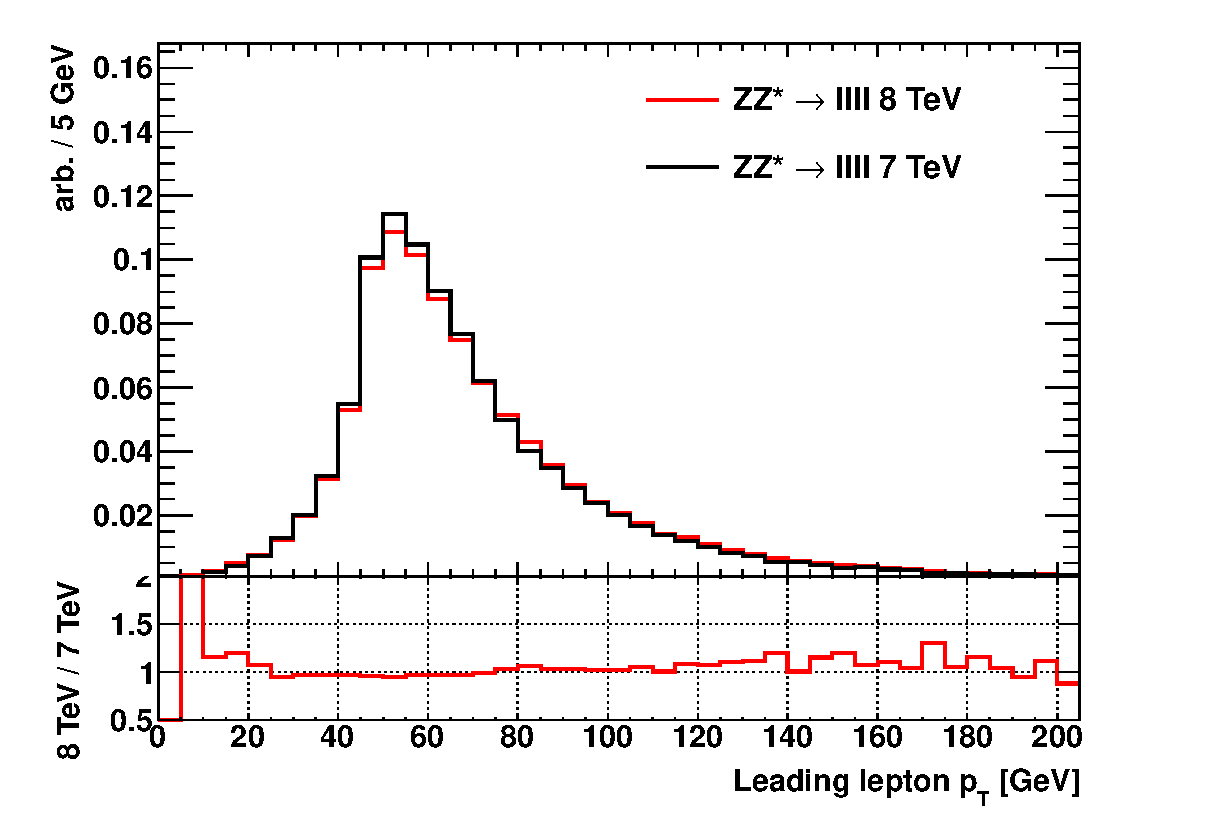
\includegraphics[width=0.47\textwidth]{Compare20112012/truth_ZZs_lep_1_pt_lin}
    }
    \subfigure[]{
        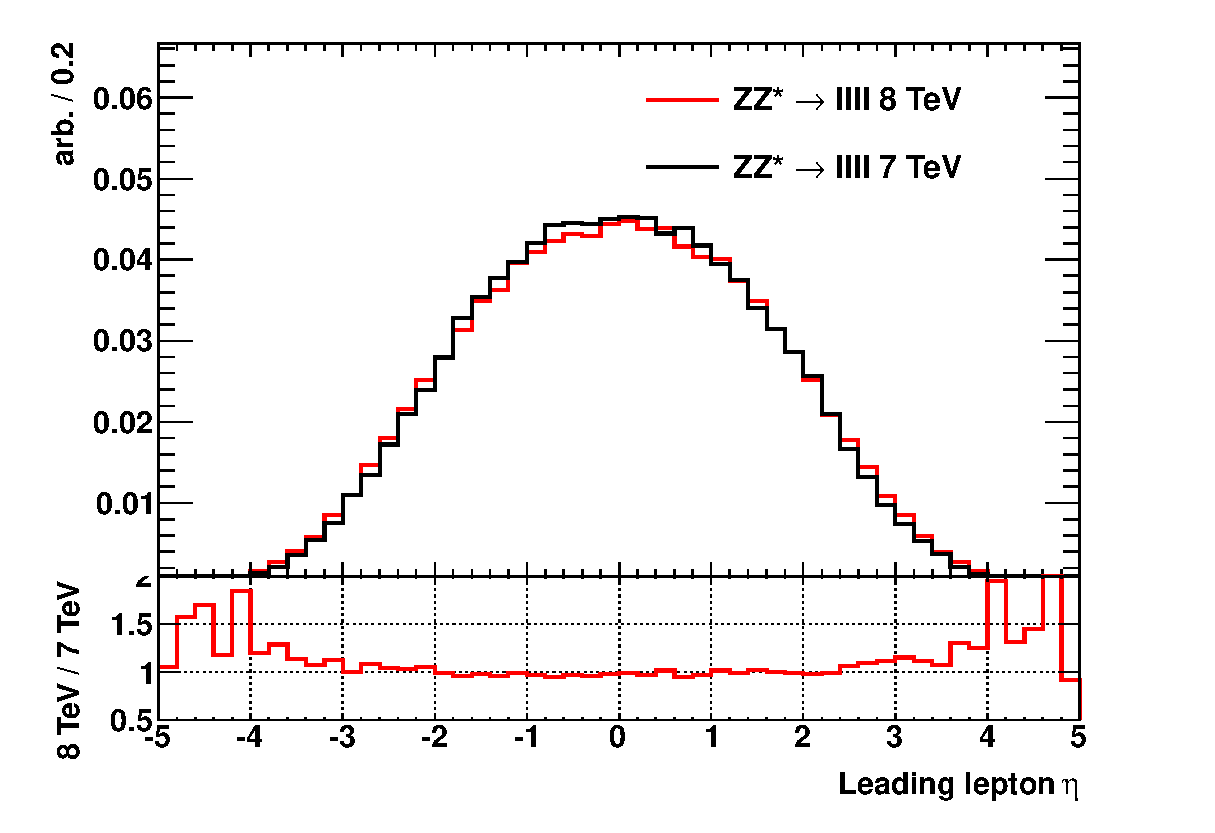
\includegraphics[width=0.47\textwidth]{Compare20112012/truth_ZZs_lep_1_eta_lin}
    }
        \vspace{-2mm}
    \subfigure[]{
        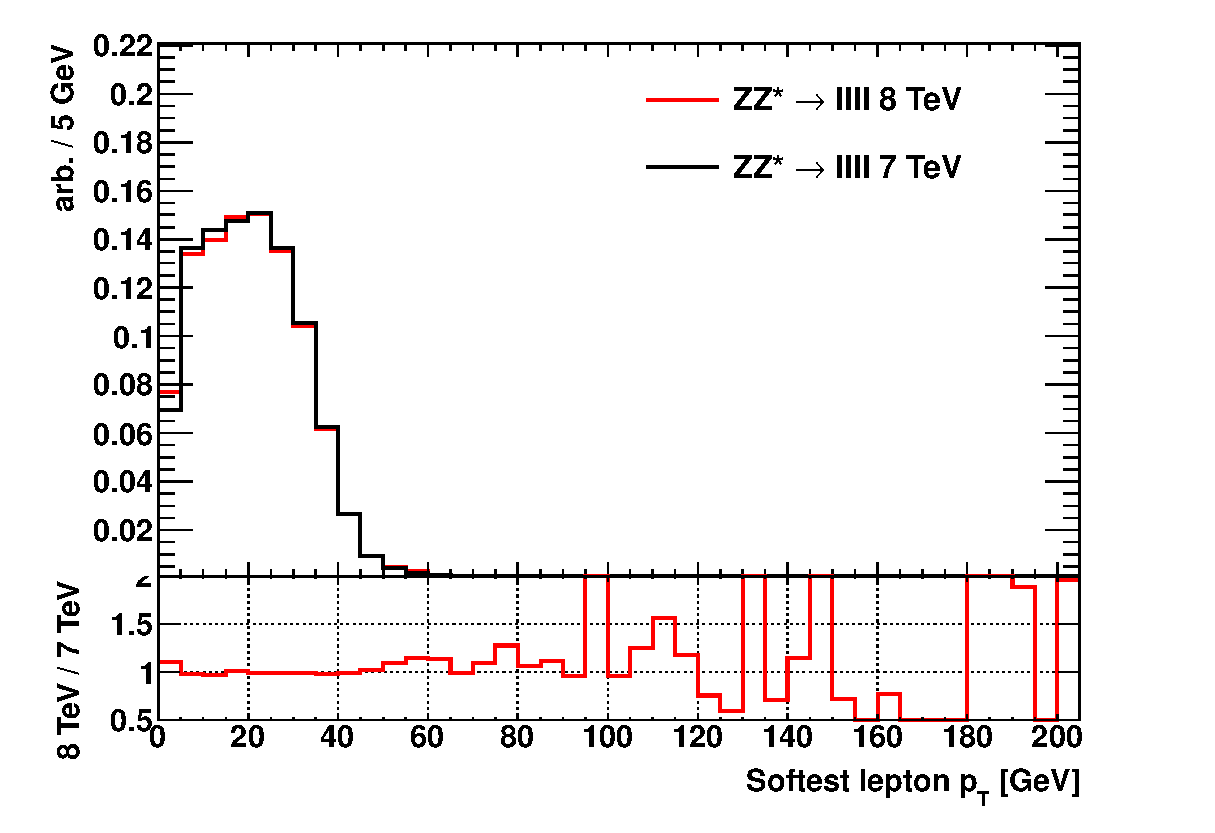
\includegraphics[width=0.47\textwidth]{Compare20112012/truth_ZZs_lep_4_pt_lin}
    }
    \subfigure[]{
        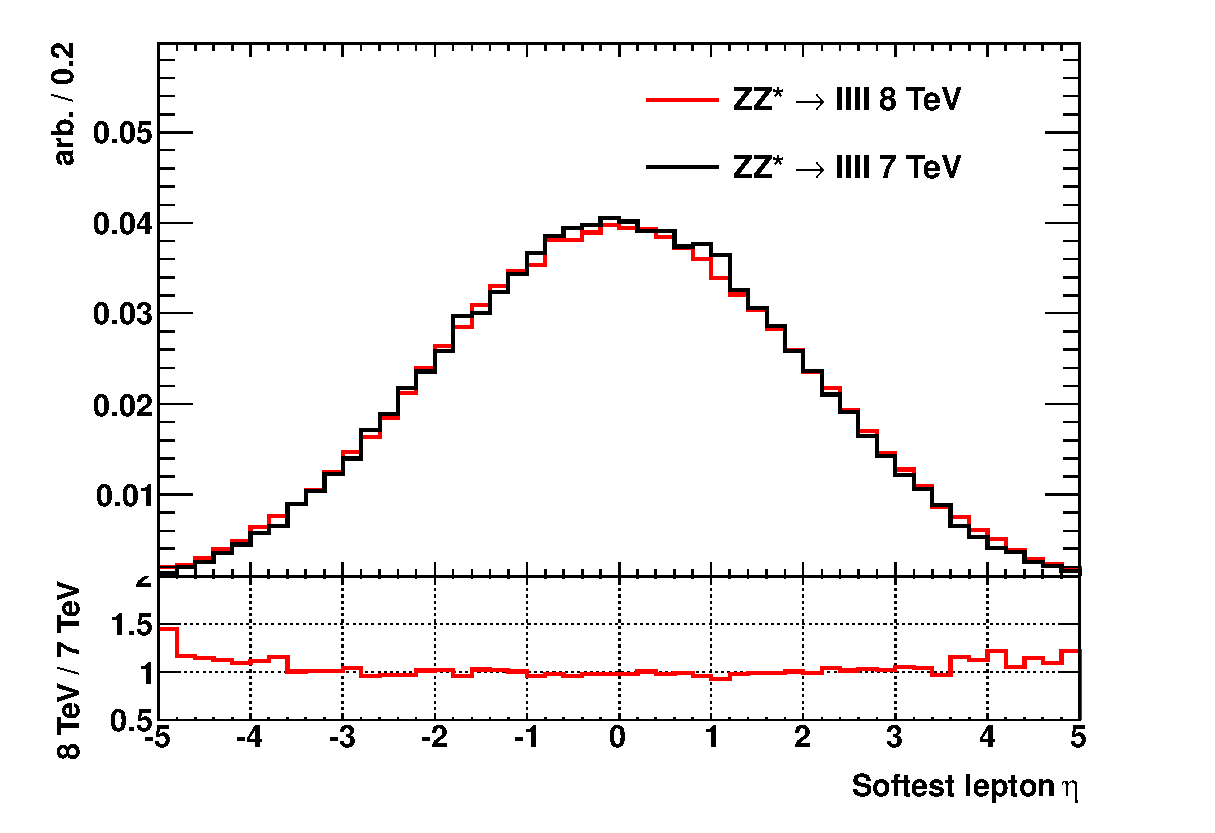
\includegraphics[width=0.47\textwidth]{Compare20112012/truth_ZZs_lep_4_eta_lin}
    }
        \vspace{-2mm}
    \caption{\small Comparison of generator level distribtuions, normalised to
    unit area, for \ZZsllll\ for 7
    \tev\ and 8 \tev. One \Z\ is required to have \sstooosZ\ and the other
    \mZgtt\. Figures (a)
    and (b) show the mass and \pt\ of the \ZZ\ system,
    respectively. Figures (c) and (d) show the \pt\ of the
    leading and subleading \Z, respectively. Figure (e) shows the \pt\ of the highest \pt\ lepton in the event, and figure (f) shows its
   $\eta$. Similarly figures (g) and (h) show the \pt\ and $\eta$ of the lowest
   \pt\ lepton in the event.}
    \label{fig:gen-comp-7-8-ZZs}
\end{figure}

\subsection{Comparison of \ggZZ\ and \qqZZ}

~\fig{gen-comp-7-8-ZZ} shows Comparison of distributions \ggZZ\ and \qqZZ.

\begin{figure}
\centering
        \vspace{-5mm}
    \subfigure[]{
        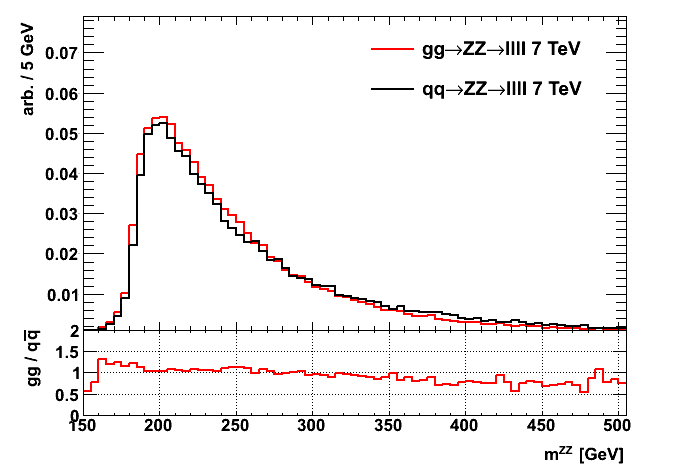
\includegraphics[width=0.47\textwidth]{Compareggqq7TeV/truth_ZZ_ZZ_m_lin}
    }
    \subfigure[]{
        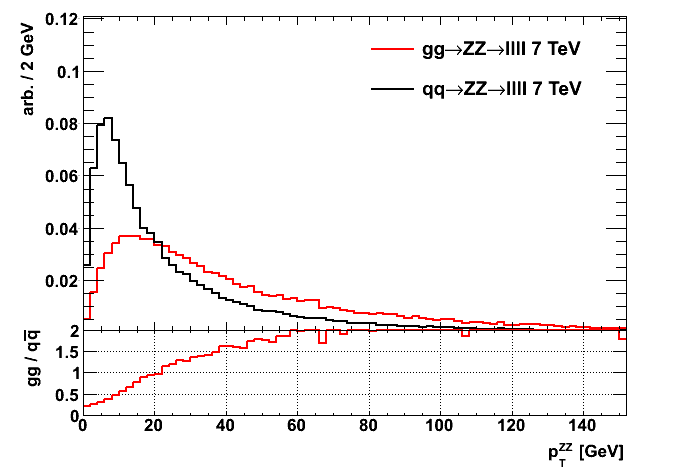
\includegraphics[width=0.47\textwidth]{Compareggqq7TeV/truth_ZZ_ZZ_pt_lin}
    }
        \vspace{-2mm}
    \subfigure[]{
        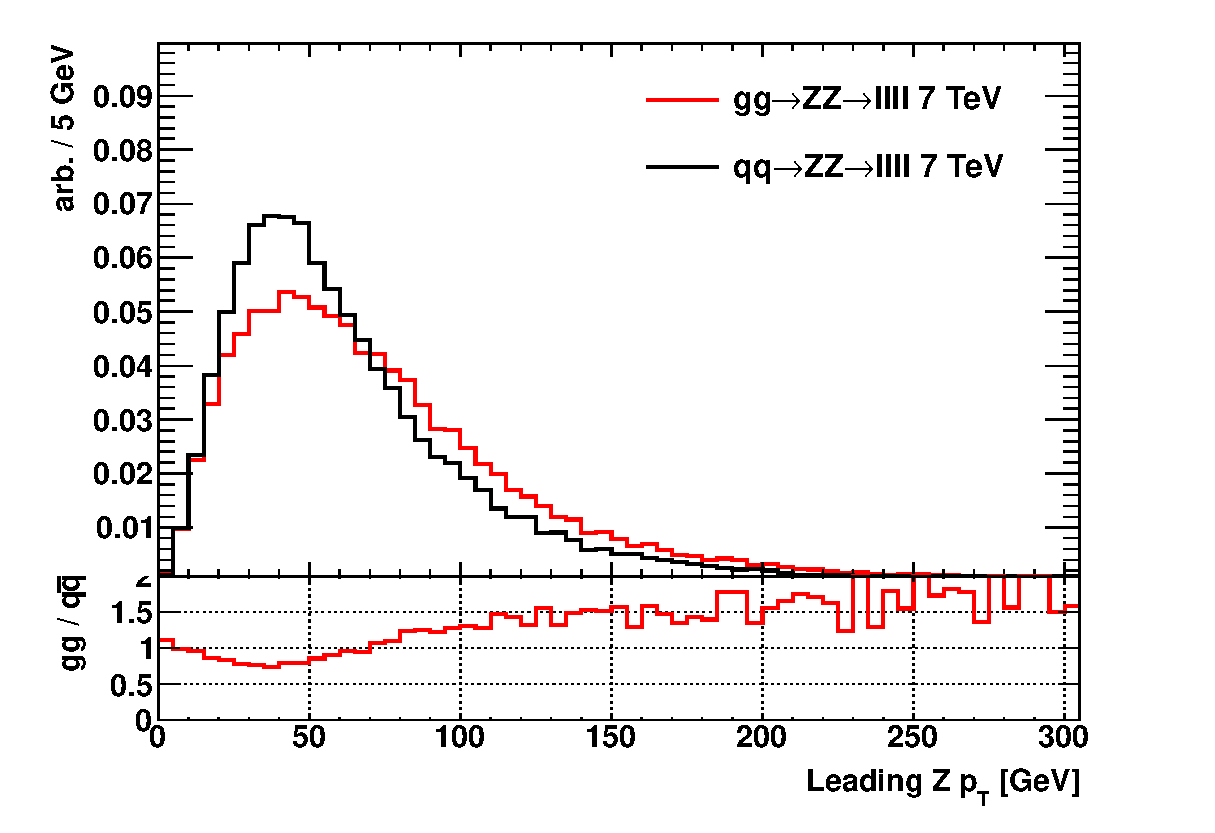
\includegraphics[width=0.47\textwidth]{Compareggqq7TeV/truth_ZZ_Z1_pt_lin}
    }
    \subfigure[]{
        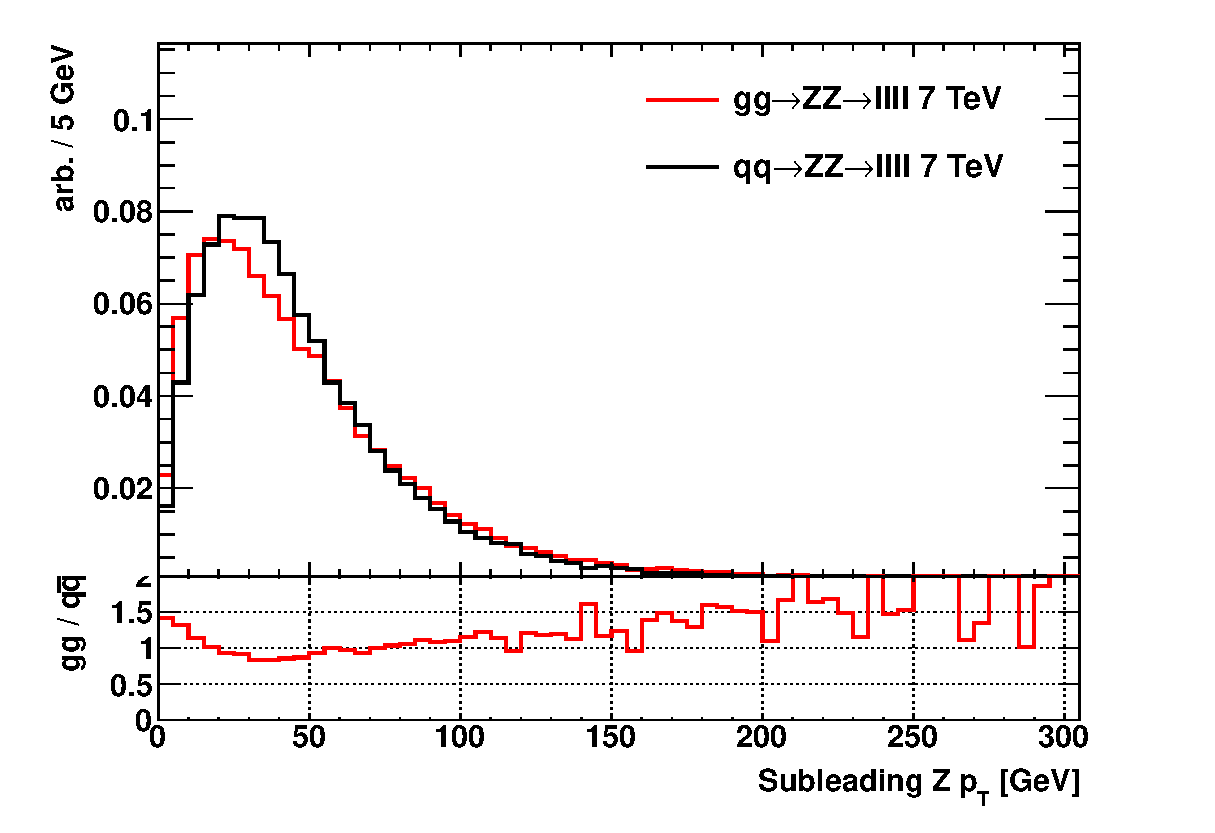
\includegraphics[width=0.47\textwidth]{Compareggqq7TeV/truth_ZZ_Z2_pt_lin}
    }
        \vspace{-2mm}
    \subfigure[]{
        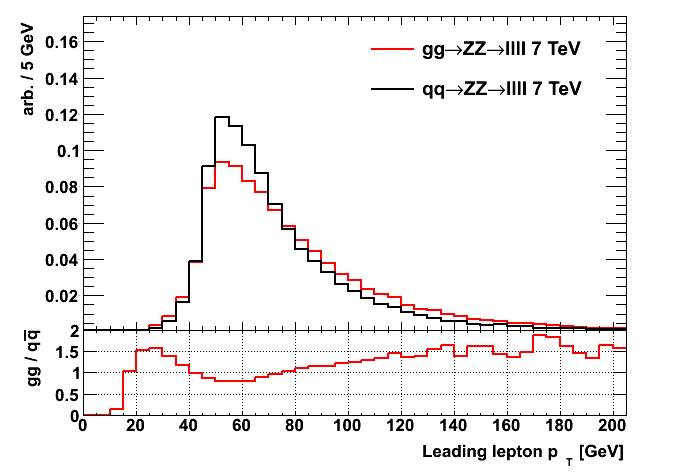
\includegraphics[width=0.47\textwidth]{Compareggqq7TeV/truth_ZZ_lep_1_pt_lin}
    }
    \subfigure[]{
        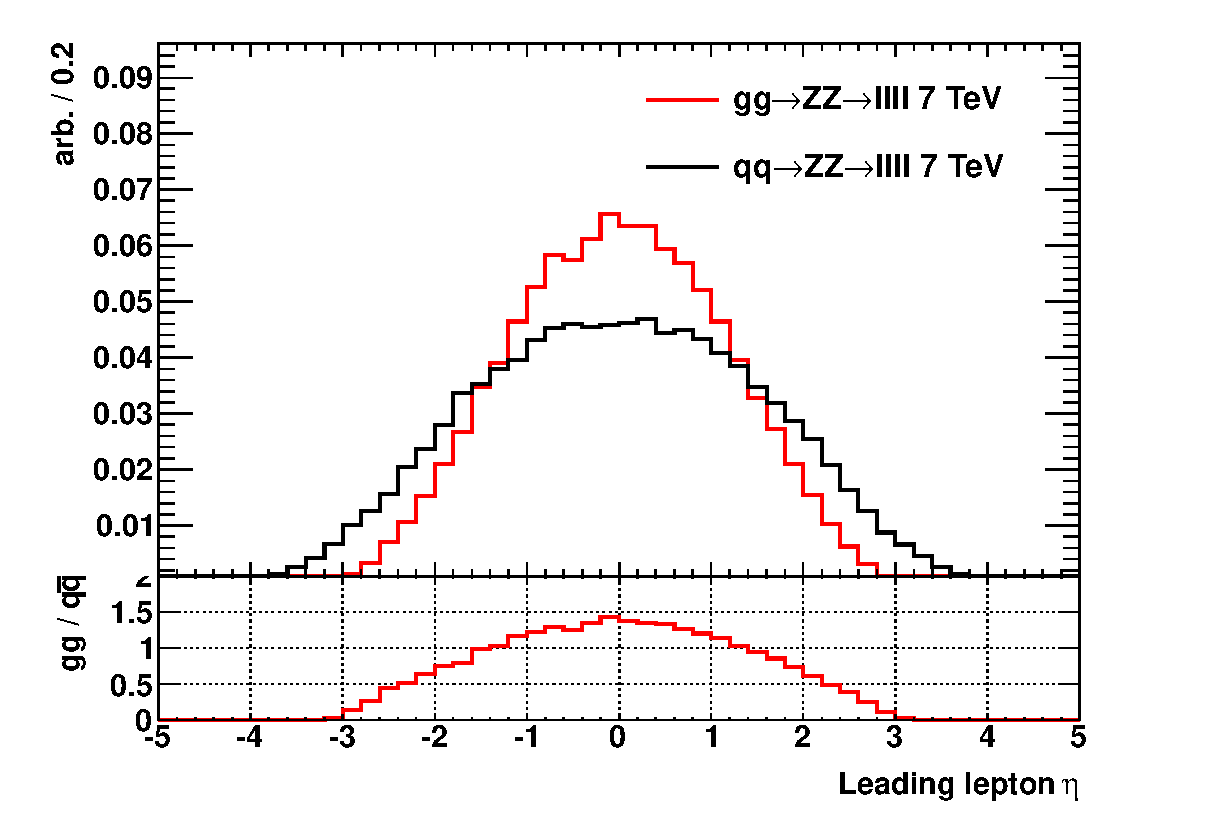
\includegraphics[width=0.47\textwidth]{Compareggqq7TeV/truth_ZZ_lep_1_eta_lin}
    }
        \vspace{-2mm}
    \subfigure[]{
        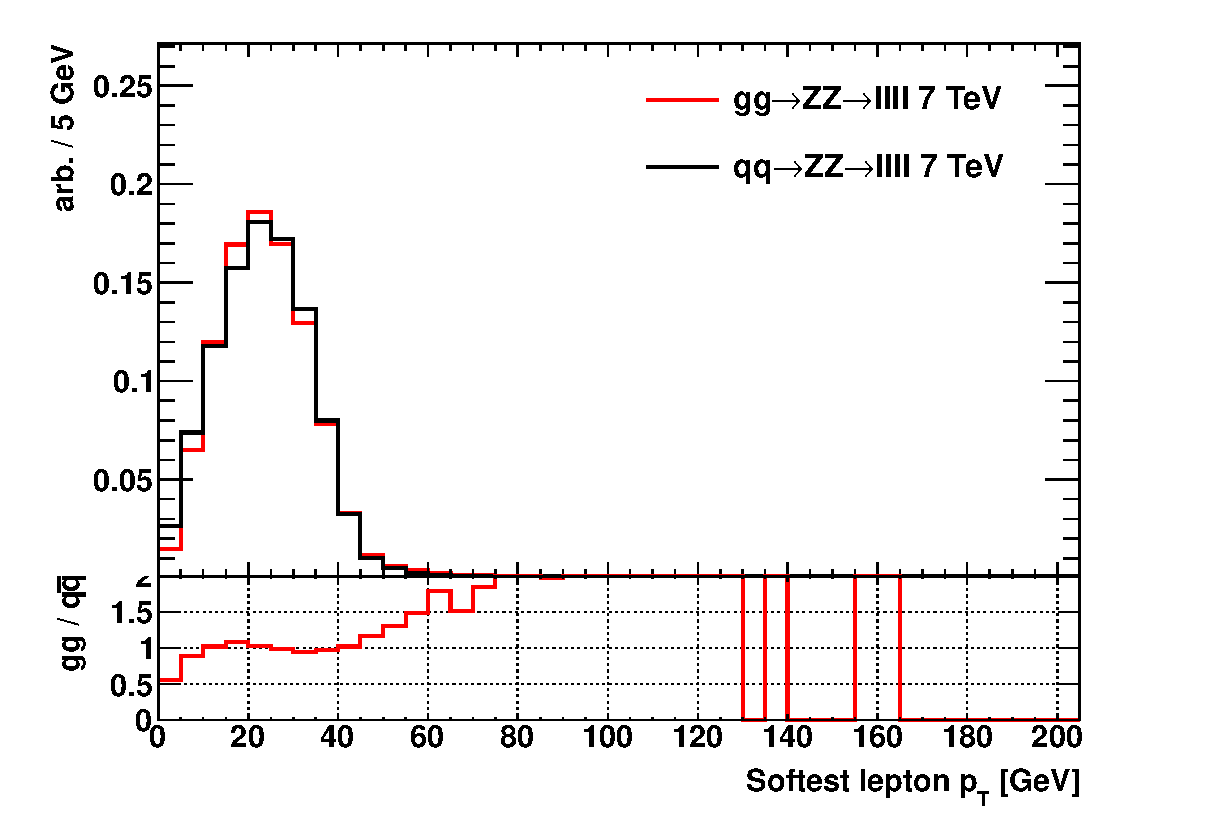
\includegraphics[width=0.47\textwidth]{Compareggqq7TeV/truth_ZZ_lep_4_pt_lin}
    }
    \subfigure[]{
        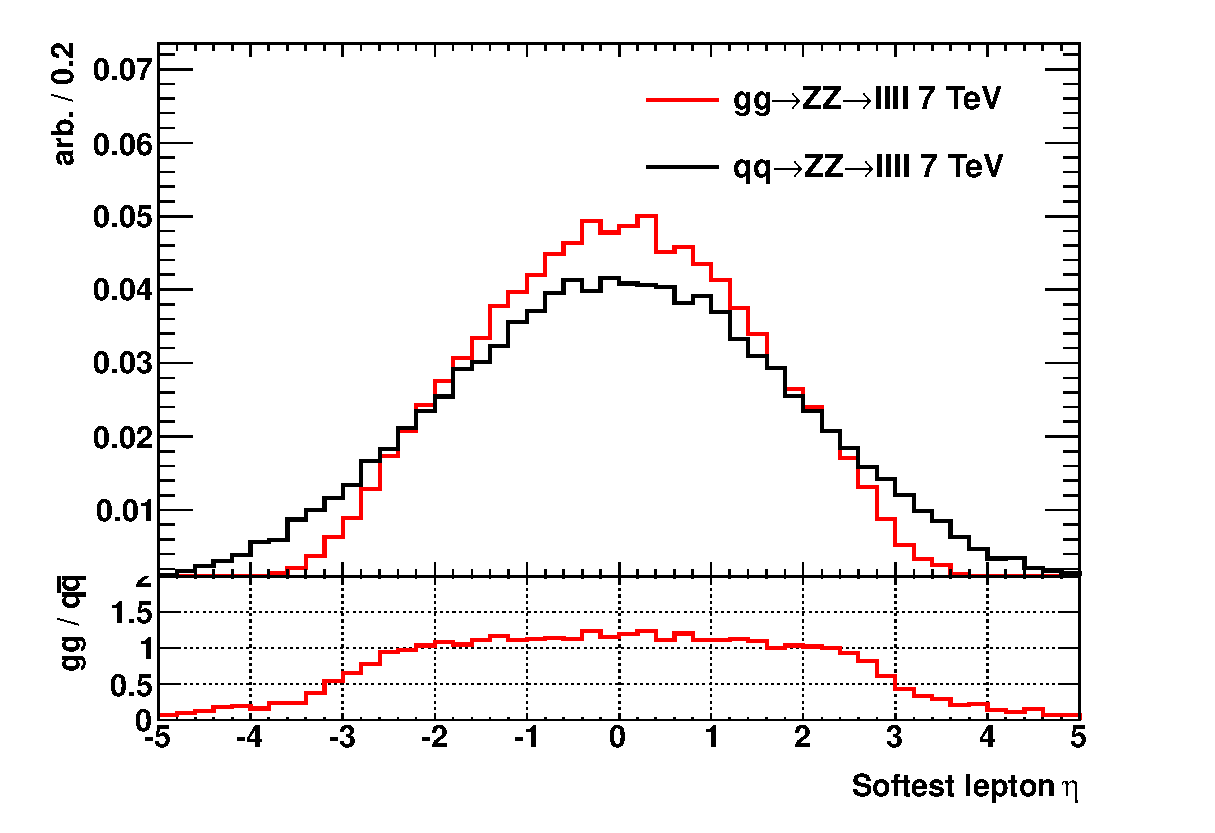
\includegraphics[width=0.47\textwidth]{Compareggqq7TeV/truth_ZZ_lep_4_eta_lin}
    }
        \vspace{-2mm}
    \caption{\small Comparison of generator level distribtuions, normalised to
    unit area, for \ZZllll\ proceeding via $qq$ and $gg$ interactions. Both \Z\
    bosons are required to have \sstooosZ. Figures (a)
    and (b) show the mass and \pt\ of the \ZZ\ system,
    respectively. Figures (c) and (d) show the \pt\ of the
    leading and subleading \Z, respectively. Figure (e) shows the \pt\ of the highest \pt\ lepton in the event, and figure (f) shows its
   $\eta$. Similarly figures (g) and (h) show the \pt\ and $\eta$ of the lowest
   \pt\ lepton in the event.}
    \label{fig:gen-comp-7-8-ZZ}
\end{figure}

\begin{figure}
\centering
        \vspace{-5mm}
    \subfigure[]{
        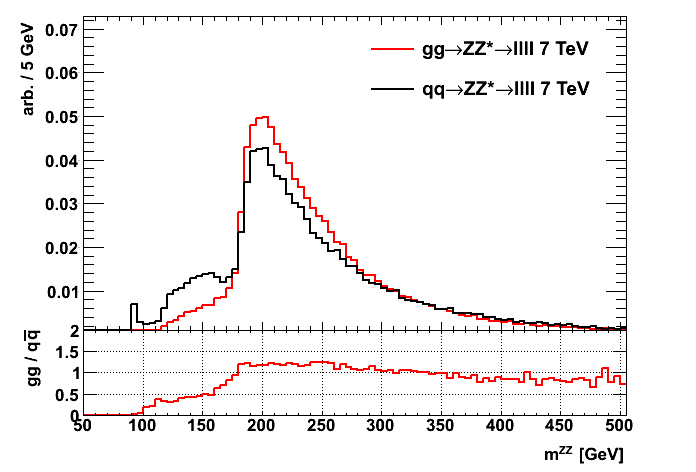
\includegraphics[width=0.47\textwidth]{Compareggqq7TeV/truth_ZZs_ZZ_m_lin}
    }
    \subfigure[]{
        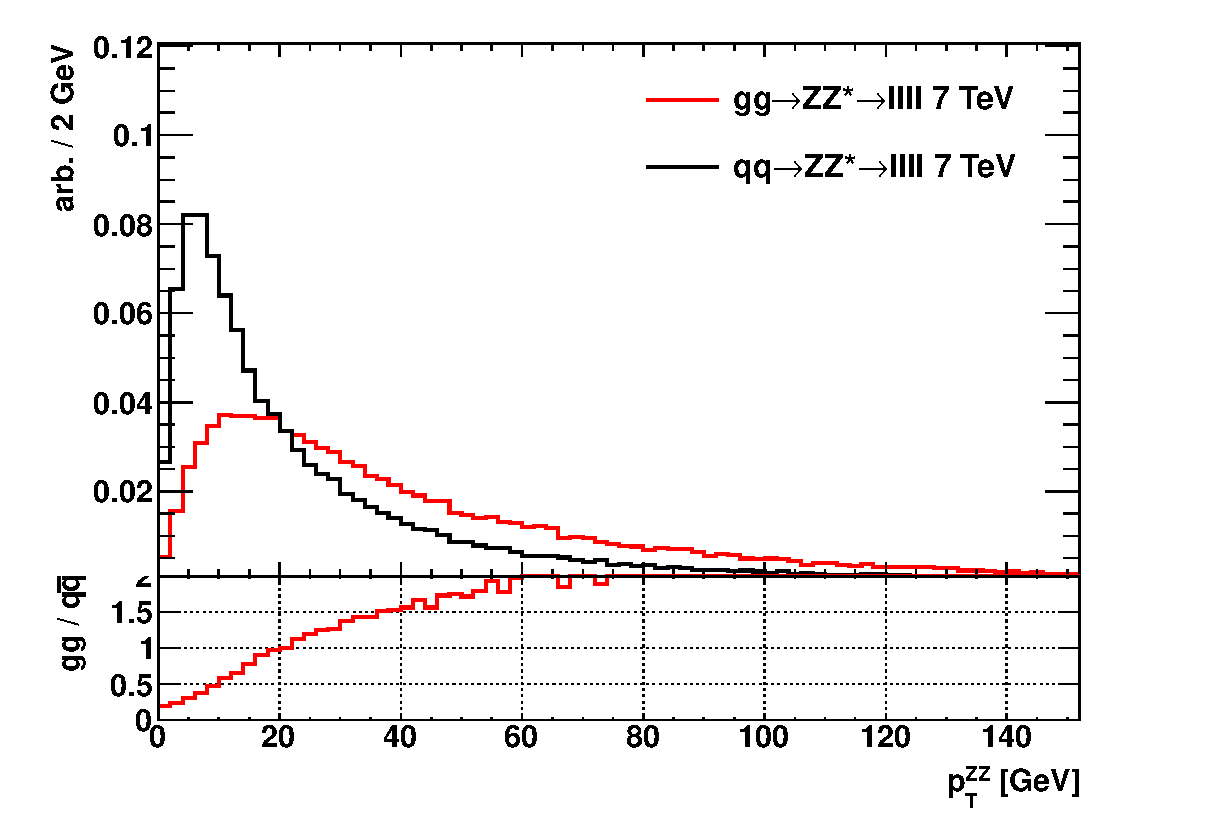
\includegraphics[width=0.47\textwidth]{Compareggqq7TeV/truth_ZZs_ZZ_pt_lin}
    }
        \vspace{-2mm}
    \subfigure[]{
        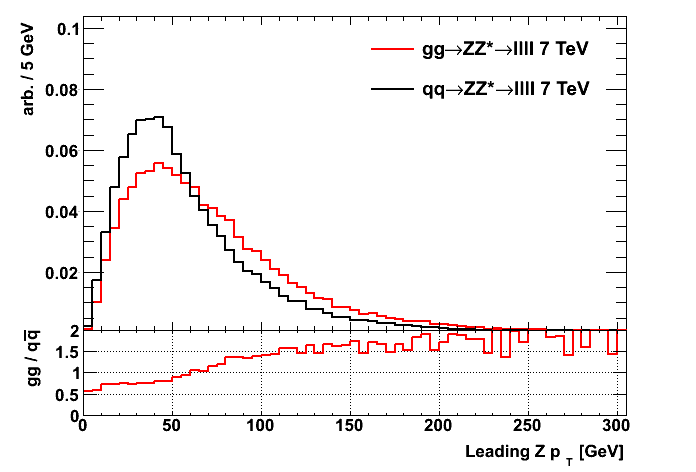
\includegraphics[width=0.47\textwidth]{Compareggqq7TeV/truth_ZZs_Z1_pt_lin}
    }
    \subfigure[]{
        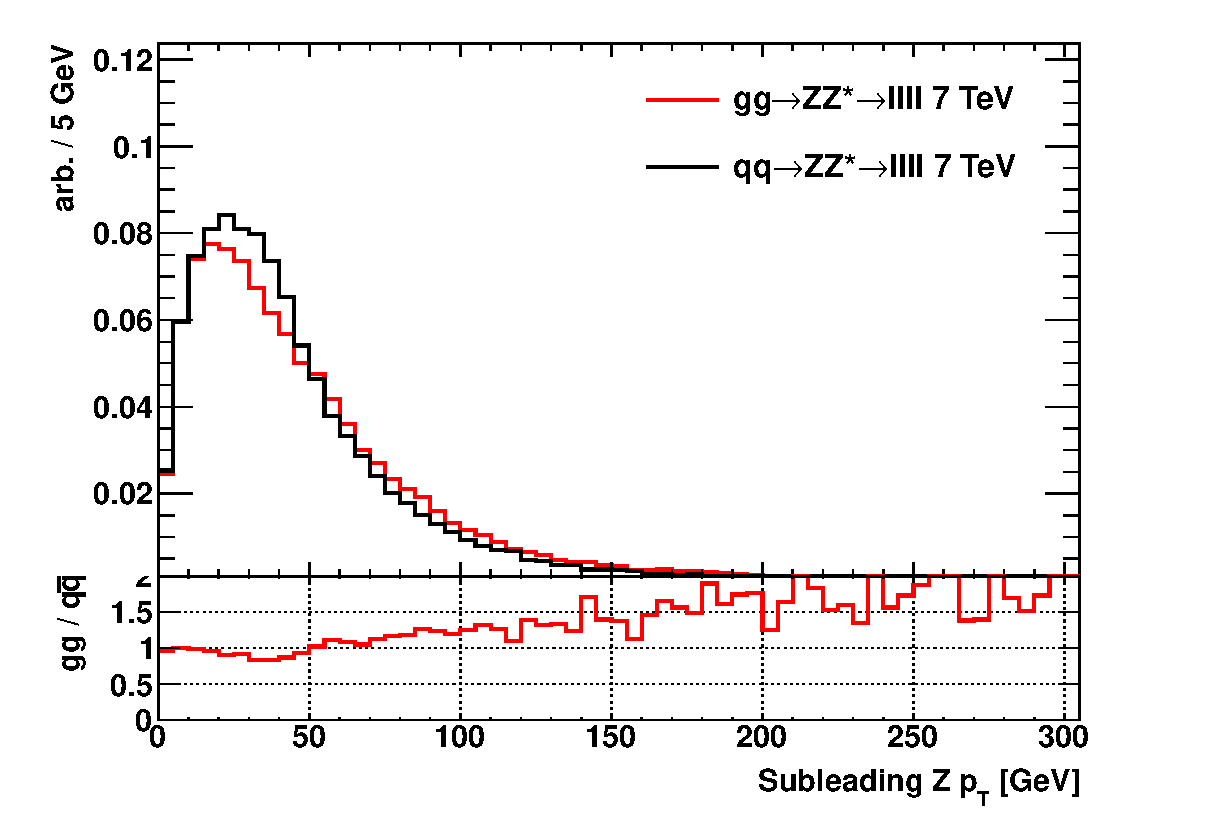
\includegraphics[width=0.47\textwidth]{Compareggqq7TeV/truth_ZZs_Z2_pt_lin}
    }
        \vspace{-2mm}
    \subfigure[]{
        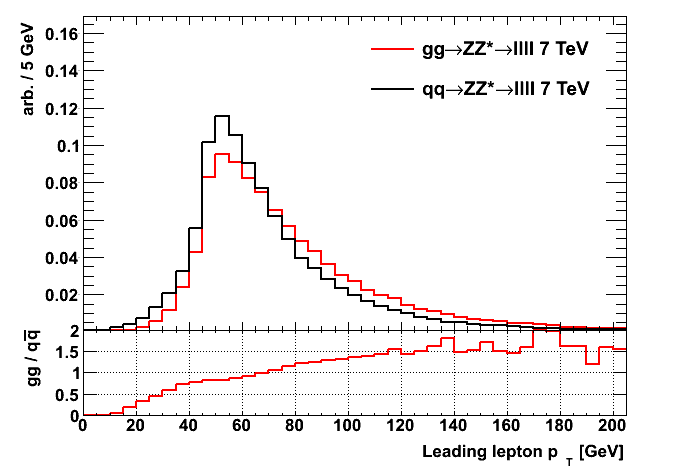
\includegraphics[width=0.47\textwidth]{Compareggqq7TeV/truth_ZZs_lep_1_pt_lin}
    }
    \subfigure[]{
        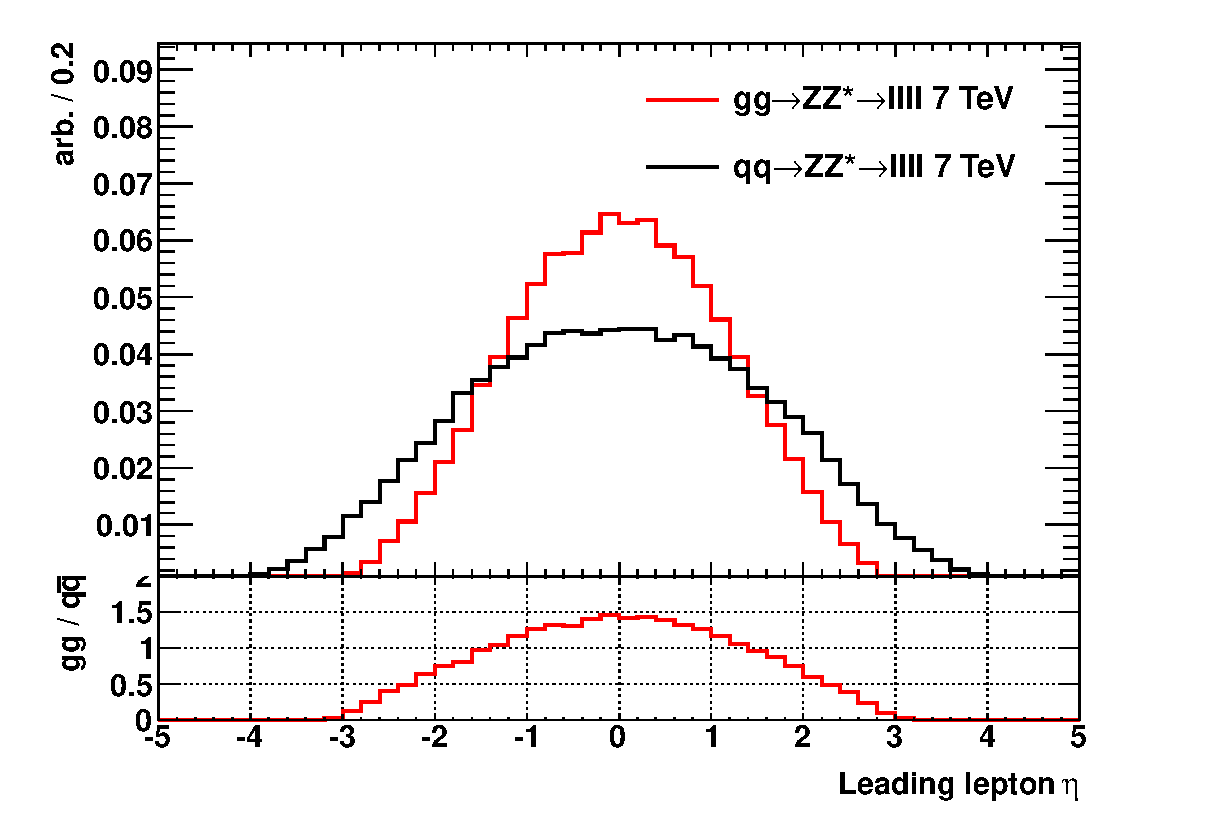
\includegraphics[width=0.47\textwidth]{Compareggqq7TeV/truth_ZZs_lep_1_eta_lin}
    }
        \vspace{-2mm}
    \subfigure[]{
        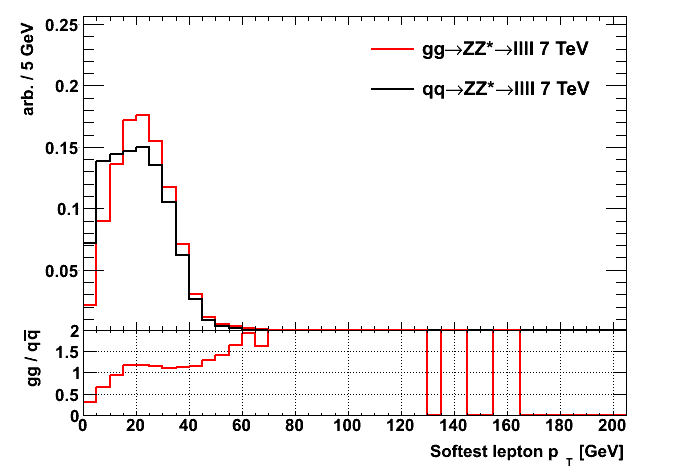
\includegraphics[width=0.47\textwidth]{Compareggqq7TeV/truth_ZZs_lep_4_pt_lin}
    }
    \subfigure[]{
        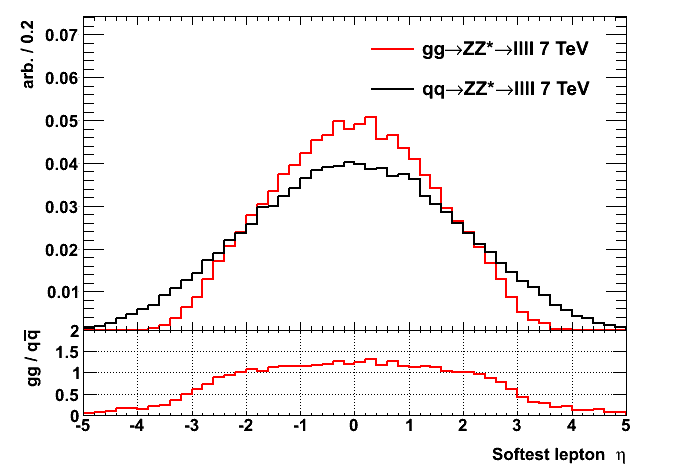
\includegraphics[width=0.47\textwidth]{Compareggqq7TeV/truth_ZZs_lep_4_eta_lin}
    }
        \vspace{-2mm}
    \caption{\small Comparison of generator level distribtuions, normalised to
    unit area, for \ZZsllll\ proceeding via $qq$ and $gg$ interactions. One \Z\ is required to have \sstooos\ and the other
    $m_{Z}>20$ \gev. Figures (a)
    and (b) show the mass and \pt\ of the \ZZ\ system,
    respectively. Figures (c) and (d) show the \pt\ of the
    leading and subleading \Z, respectively. Figure (e) shows the \pt\ of the highest \pt\ lepton in the event, and figure (f) shows its
   $\eta$. Similarly figures (g) and (h) show the \pt\ and $\eta$ of the lowest
   \pt\ lepton in the event.}
    \label{fig:gen-comp-7-8-ZZs}
\end{figure}


\subsection{Generator Comparisons for \ZZllll}

\begin{figure}
\centering
        \vspace{-5mm}
    \subfigure[]{
        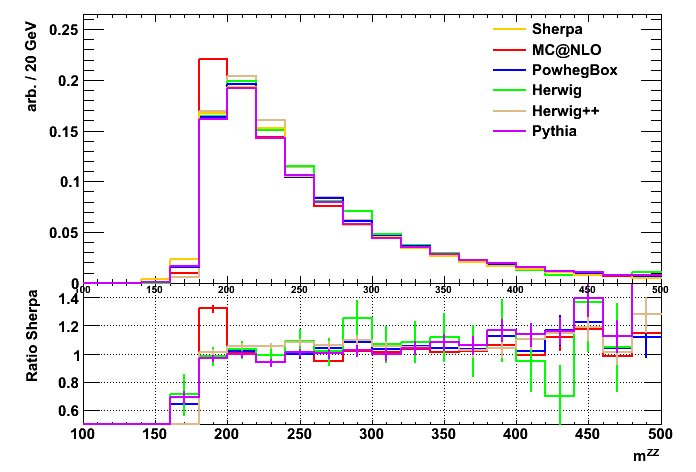
\includegraphics[width=0.47\textwidth]{GeneratorComparison/fidZZ_ZZ_m_2e2mu_wRatio_linear}
    }
    \subfigure[]{
        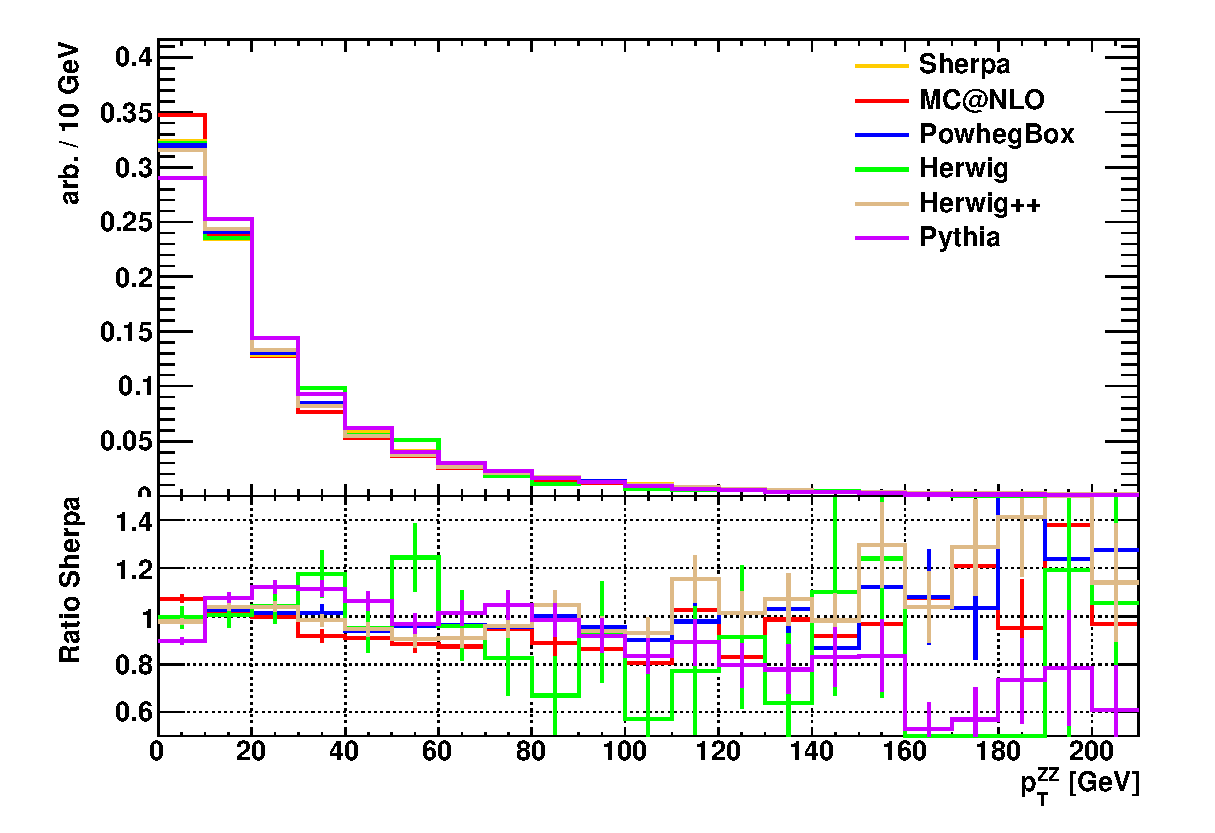
\includegraphics[width=0.47\textwidth]{GeneratorComparison/fidZZ_ZZ_pt_2e2mu_wRatio_linear}
    }
        \vspace{-2mm}
    \subfigure[]{
        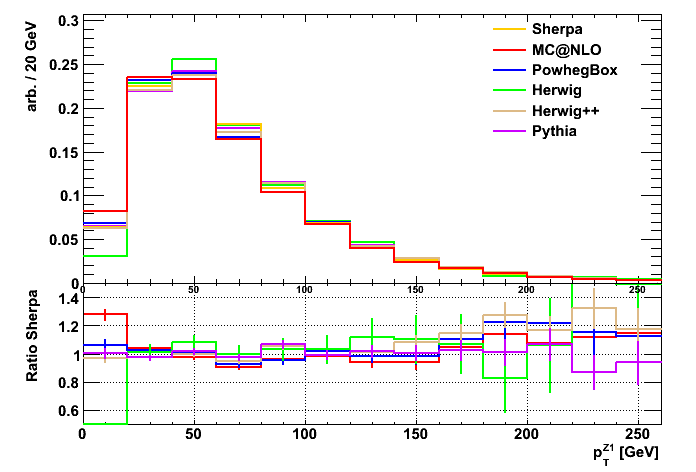
\includegraphics[width=0.47\textwidth]{GeneratorComparison/fidZZ_Z1_pt_2e2mu_wRatio_linear}
    }
    \subfigure[]{
        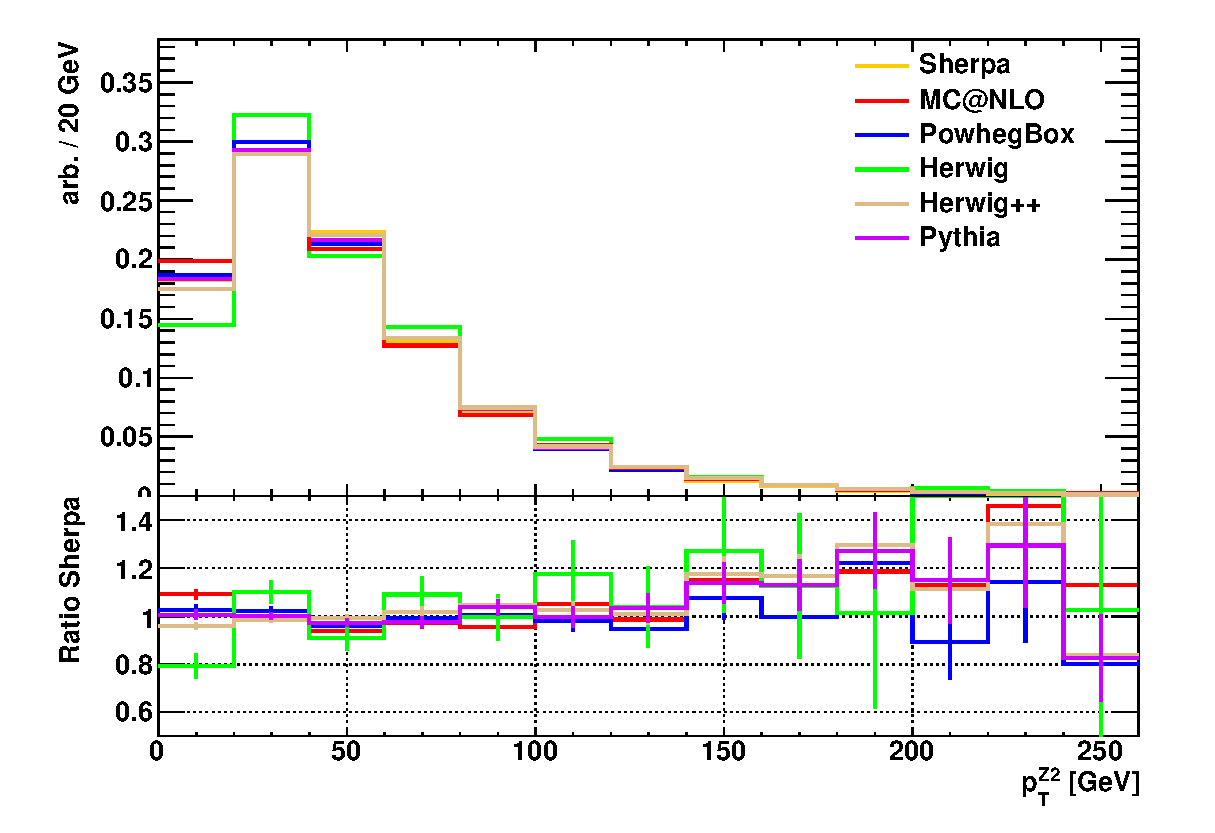
\includegraphics[width=0.47\textwidth]{GeneratorComparison/fidZZ_Z2_pt_2e2mu_wRatio_linear}
    }
        \vspace{-2mm}
    \subfigure[]{
        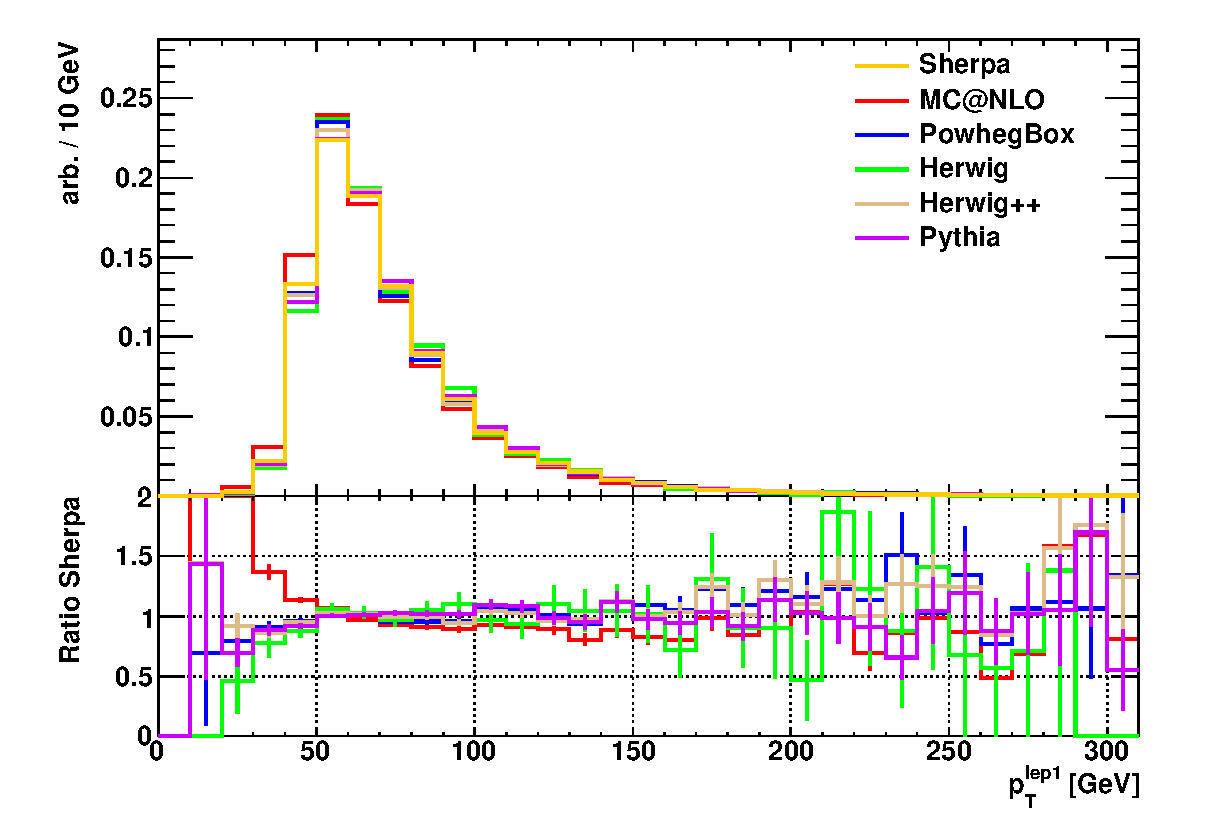
\includegraphics[width=0.47\textwidth]{GeneratorComparison/ZZ_lep_1_pt_2e2mu_wRatio_linear}
    }
    \subfigure[]{
        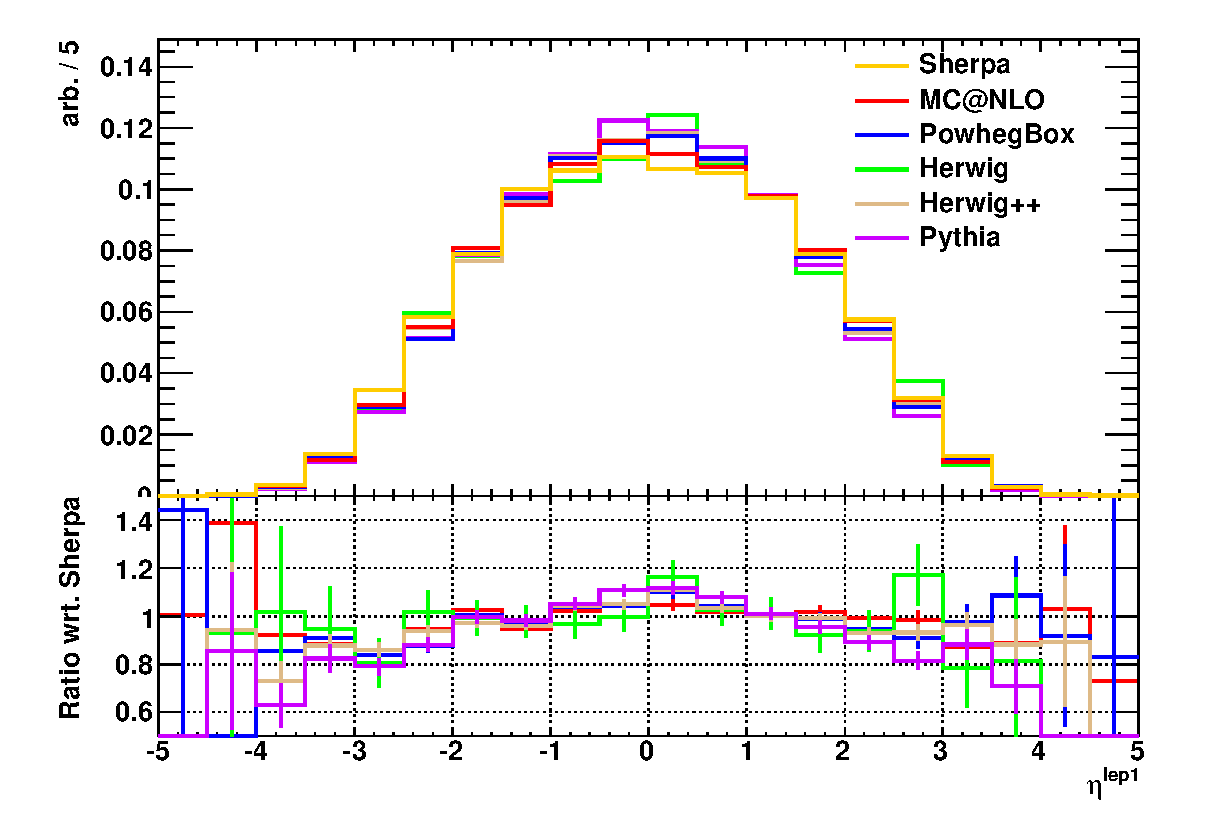
\includegraphics[width=0.47\textwidth]{GeneratorComparison/ZZ_lep_1_eta_2e2mu_wRatio_linear}
    }
        \vspace{-2mm}
    \subfigure[]{
        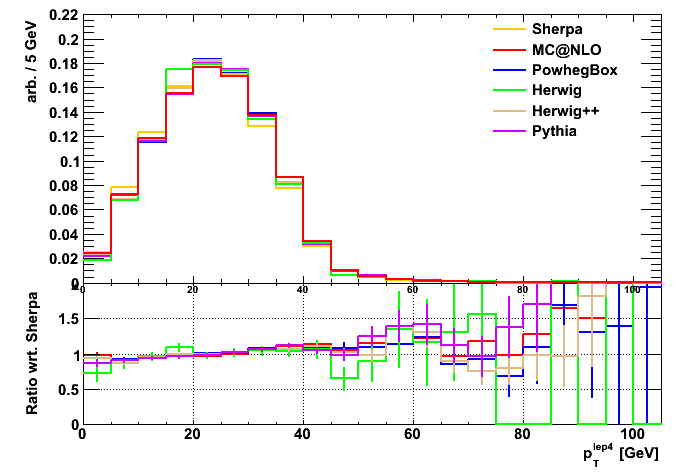
\includegraphics[width=0.47\textwidth]{GeneratorComparison/ZZ_lep_4_pt_2e2mu_wRatio_linear}
    }
    \subfigure[]{
        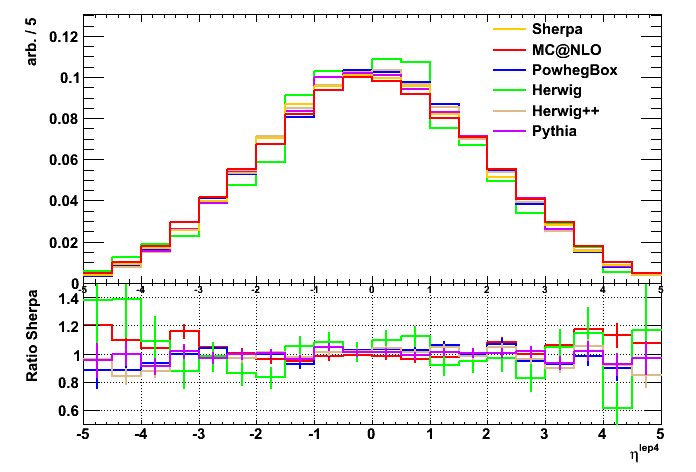
\includegraphics[width=0.47\textwidth]{GeneratorComparison/ZZ_lep_4_eta_2e2mu_wRatio_linear}
    }
        \vspace{-2mm}
    \caption{\small Comparison of generator level distribtuions, normalised to
    unit area, for \ZZsllll\ proceeding via $qq$ and $gg$ interactions. One \Z\ is required to have \sstooos\ and the other
    $m_{Z}>20$ \gev. Figures (a)
    and (b) show the mass and \pt\ of the \ZZ\ system,
    respectively. Figures (c) and (d) show the \pt\ of the
    leading and subleading \Z, respectively. Figure (e) shows the \pt\ of the highest \pt\ lepton in the event, and figure (f) shows its
   $\eta$. Similarly figures (g) and (h) show the \pt\ and $\eta$ of the lowest
   \pt\ lepton in the event.}
    \label{fig:gen-comp-7-8-ZZs}
\end{figure}


%% TGC diagram
%\begin{figure}
%\centering
%        \vspace{10mm}
%    \mbox{
%    \subfigure{
%        \begin{fmffile}{schan}
%        \begin{fmfgraph*}(36,20)
%            \fmfleft{i1,i2}
%        \fmfright{o1,o2}
%        \fmflabel{$u,d$}{i2}
%        \fmflabel{$\bar{u},\bar{d}$}{i1}
%        \fmfright{o1,o2}
%        \fmflabel{$Z/\gamma^{*}$}{o1}
%        \fmflabel{$Z/\gamma^{*}$}{o2}
%        \fmf{fermion}{i2,v1,i1}
%        %\fmf{fermion}{v2,i2}
%        %\fmf{fermion}{v1,i1}
%        \fmf{photon,label=$Z/\gamma^{*}$}{v1,v2}
%        \fmf{photon}{v2,o1}
%        \fmf{photon}{v2,o2}
%        % uncommment this line if you want dots at the vertices
%            %\fmfdotn{v}{4}
%        \end{fmfgraph*}
%        \end{fmffile}
%    }
%    }
%        \vspace{5mm}
%    \caption{A diagram!}
%\end{figure}

The difference in the \Z\ line-shape observed between \sherpa\ and the other
generators is attributed to the fact that \sherpa\ applies QED FSR in a
different way. For all of the other generators compared in ??, \photos\cite{Golonka:2005pn} is used
to model QED radiation, whereas \sherpa\ has it's own internal treatment. There are two
ways of applying QED radiation to a \ZZllll\ final state. The radiation can
either be applied from the full \llll\ multipole, distributing the recoil within
the multipole, or assuming two separate dipoles, $\Z[\ell\ell]$ and
$\Z[\ell'\ell']$, each
of which undergoes QED radiation independently from each other. The latter
treatment leaves the mass of each dilepton pair invariant, whereas the former
treatment leaves the mass of the four-lepton system invariant. \photos\ uses the
$(\ell\ell)(\ell'\ell')$ approach, whilst the \sherpa\ samples used in Figure ??
use the $(\llll)$ approach. ~\fig{??} shows the difference between the \Z\
lineshape in \sherpa\ samples generated using the two approaches; the \Z\
lineshape in \sherpa\ samples generated using the $(\ell\ell)(\ell'\ell')$ approach agree with the productions from the generators using \photos. It is not  clear which is the correct approach
theoretically~\cite{Siegert}, so additional systematics are assigned to account
for differences resulting from the two approaches.

%
\section{Previous experimental results}

Diboson ZZ production was first observed in $e^+e^-$ collisions at LEP in 1997.
The L3 experiment published the first observation and \cx\ measurement
of on-shell \ZZ\ production~\cite{Acciarri1999281}. They analysed 55.3 \ipb\
of data collected at an average centre-of-mass energy of 182.7 GeV. Separate
selections were applied in the various decay channels. Whilst no events were
observed in the $\ell\ell\ell\ell$ final states, a total of 63 were observed in
the other visible final states. The majority (47) of these were in the
all-hadronic channel, which suffered from high backgrounds from $e^+e-
\rightarrow qq \gamma$ and $e^+e- \rightarrow WW$. In this channel a neural
network method was used to distinguish the signal events from the background. A
log-likelihood fit of the neural network output and the observed mass spectra in
the other channels was used to combine the channels, and gave a \cx\ of
$\sigma_{ZZ} = 0.30^{+0.22 +0.07}_{-0.16 -0.03}$, in very good agreement with
the standard model prediction. The data were fitted to determine the magnitude
of the anomalous triple gauge couplings. These were found to be consistent with
the SM predictions of 0 to 95\% confidence level. Updated \cx\
measurements have since been published by L3 and the other 3 LEP experiments, in
all cases measuring \cx s for \ZZ\ production consistent with the
standard model, and finding no evidence for anomalous couplings.

Measurements of the \ZZ\ \cx\ have also been made in $p \bar{p}$
collisions at a centre of mass energy of $\sqrt{s} = 1.96$ \tev\ at the Tevatron, at
both the D0 and the CDF experiments. The most recent D0 publication reports the
observation of 10 candidate \ZZ\ events with an expected background of $0.37
\pm 0.13$. The measured \cx\ was $1.33^{+0.5}_{-0.4}$ (stat) $\pm$ 0.12
(syst) $\pm$ 0.09 (lumi) pb, with a signal significance of greater than
$6\sigma$. The result is consistent with the standard model prediction of 1.4
$\pm$ 0.1 pb. 

%The \cx\ at the LHC for a centre-of-mass energy of 7 \TeV\ is predicted to be $\sim$5 times larger 
%than at the Tevatron. 
Recently the CMS experiment have measured the \ZZ\ production cross
section~\cite{CMS-PAS-EWK-11-010} and found it consistent with the Standard Model prediction.


\section{Anomolous Triple Gauge Couplings}
Non-zero nTGCs would manifest as an increased \ZZ\
production \cx, especially at high \ZZ\ invarient mass and transverse
momentum~\cite{Baur:2000ae}.

\section{ZZ Resonances}


\part{Experimental Description}
\graphicspath{{Chapters/Detector/Figures/}}
\chapter{The ATLAS Detector at the LHC}
\label{chap:Detector}

\section{The Large Hadron Collider}

The Large Hadron Collider (LHC) is a particle accelerator located at CERN, the
European Organisation for Nuclear Research, on the French-Swiss border near
Geneva. The LHC is the world's most powerful particle accelerator, colliding
beams of protons together at centre of mass energies of up to 8 \TeV, with the
aim of better understanding the workings of our Universe. It is installed in a
tunnel of circumference 26.7 km, which previously held the Large
Electron-Positron Collider (LEP), and is between 45 and 170 m below the ground.
The beams are brought to collision at four points around the ring, at each of
which a different experiment is located. The machine is also capable of
colliding heavy ions, providing a complementary heavy-ion physics program.

The design of the LHC is described in detail in ~\cite{1748-0221-3-08-S08001}
and ~\cite{Brüning:782076}. A brief summary is given in~\ref{sec-lhc-design},
and details of LHC operations in 2011 and 2012 are given
in~\ref{sec-lhc-operation}.

\subsection{Machine Design}
\label{sec-lhc-design}

In normal operating mode, the LHC contains two counter-circulating beams of protons. 
Since the beams are of similarly charged particles
orbiting in opposite directions, they require opposite bending fields, thus need
to be in separate beam-pipes. Due to space and cost constraints, the two beam-pipes are
contained within a single structure incorporating a twin bore superconducting
magnet. Superconducting dipole magnets are
used to bend the beams and keep them in orbit and superconducting quadrupole magnets are used to
keep the beams focussed. The magnets must be cooled to 2K to retain their superconducting
properties; this is achieved with a helium-based cooling system. 

Protons are injected into the LHC from the SPS (Super Proton Synchrotron) in
bunches, at a centre of mass energy of 450 \GeV. They are then accelerated to the desired
collision energy by means of superconducting Radio Frequency (RF) cavities. Once the
particles are accelerated to full energy, the RF cavities are used to keep the
particles in their bunches. The bunches are brought to collision at four points
around the ring, at each of which a different experiment is located. The ATLAS
experiment at Point 1 and the CMS experiment at Point 5 are general purpose
detectors, and the LHCb experiment at Point 8 and ALICE at Point 2 are
specialised detectors studying heavy-flavour physics and heavy-ion collisions
respectively.

%The ATLAS experiment sits at
%point 1, the ALICE experiment at Point 2, the CMS experiment at Point 5, and the
%LHCb experiment at Point 8 (the remaining `Points' are access locations to the
%ring).

The rate at which collisions occur depends on the instantaneous luminosity
$\mathcal{L}$ and the collision \cx\ $\sigma$, related by:

\begin{equation}
\frac{dN}{dt} = \mathcal{L} \cdot \sigma
\end{equation}

The total \cx\ for
proton-proton collisions at the LHC has been measured to be
\measStatSyst{98.3}{\errSym{0.2}}{\errSym{2.8}}~mb\footnote{$1 \rm{b} = 10^{-28}
m^{2}$} at a centre of mass energy of 7 \tev~\cite{0295-5075-96-2-21002}, thus
at the LHC design luminosity of $1 \times 10^{34}~\rm{cm}^{-2}\rm{s}^{-1}$
collisions occur at a rate of approximately 100 MHz. 

The rate at which a particular
physics process occurs depends on the \cx\ for the process in question.
Since many of the physics processes under study at the LHC are very rare and
have small \cx s, it is important to maximise the luminosity as much as
possible. The instantaneous luminosity is approximately given by:
%(neglecting relativistic effects for clarity):

\begin{equation}
\mathcal{L} = \frac{N_{\rm{b}}^{2}n_{\rm{b}}f_{\rm{rev}}\gamma_{\rm{r}}}{4\pi
\epsilon_{n}\beta^{*} F}
\end{equation}

where:

\begin{itemize}
    \item $N_{\rm{b}}$ is the number of particles per bunch,
    \item $n_{\rm{b}}$ is the number of bunches per beam, 
    \item $f_{\rm{rev}}$ is the revolution frequency, 
    \item $F$ is a geometric function to account for the crossing angle between the beams (since
they are generally not collided head on), 
    \item $\epsilon_{n}$ is the beam emittance,
a measure of how uniform the momentum of particles in the beam is or how small
the beam can be `squeezed',
    \item $\beta^{*}$ is a measure of how narrow the beam is at the interaction
    point, or how `squeezed' it is,
    \item $\gamma_{r}$ is the relativistic Lorentz factor $(1 -
    v^2/c^2)^{-\frac{1}{2}}$.
\end{itemize}
    
The \cx\ of the beam at
the interaction point is proportional to ${\epsilon_{n} \cdot \beta^{*}}$.
The instantaneous luminosity can be maximised by increasing the
number of particles per bunch, decreasing the bunch spacing (or equivalently
increasing the number of bunches per beam) or decreasing the size of the bunch
at the interaction point by decreasing $\epsilon_{n}$ and $\beta^{*}$.

A measure of how many collisions have occurred is the integrated luminosity:

\begin{equation}
L = \int \mathcal{L} \, dt
\end{equation}

The number of events occurring for a given process with \cx\
$\sigma_{\rm{process}}$ in a data sample corresponding to an integrated
luminosity $L$ is given by:

\begin{equation}
N_{\rm{process}} = L \cdot \sigma_{\rm{process}}
\end{equation}

\subsection{LHC Operation in 2011 and 2012}
\label{sec-lhc-operation}

The LHC began operation in November 2009 with collisions at a centre of mass
energy of 900~\GeV, with the centre of mass energy rising to a world record
2.36~\TeV\ by the end of the year. In 2010 the centre of mass energy was
successfully increased to 7~\TeV. Over 2010 and 2011 the LHC continued to run at
\sqrts{7}, with the instantaneous luminosity steadily increasing. In 2010 the
LHC delivered \LumiTotalDeliveredTwentyTen\ of integrated luminosity to ATLAS
and delivered \LumiTotalDeliveredTwentyEleven\ in 2011. In 2012 the centre of mass energy was
increased to 8 \tev, and the instantaneous luminosity further increased by
increasing the number of particles per bunch slightly and decreasing
$\epsilon_{n}$ and $\beta^{*}$, leading to a total integrated luminosity
delivered to ATLAS in 2012 of \LumiTotalDeliveredTwentyTwelve. 

\begin{figure}[h]
\centering
            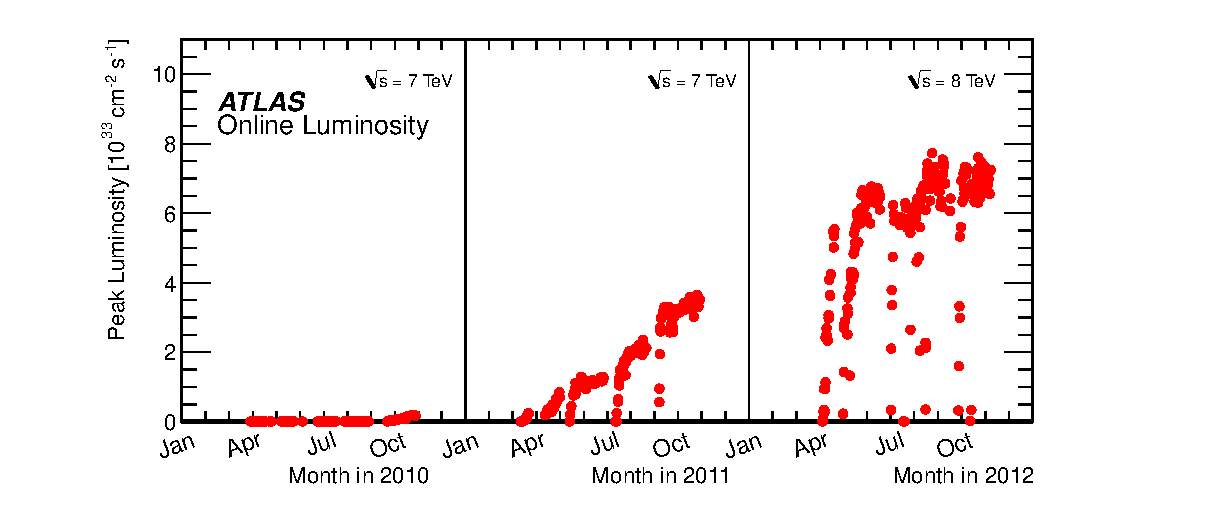
\includegraphics[width=\textwidth]{lumivstime}
%	\subfigure[]{
%            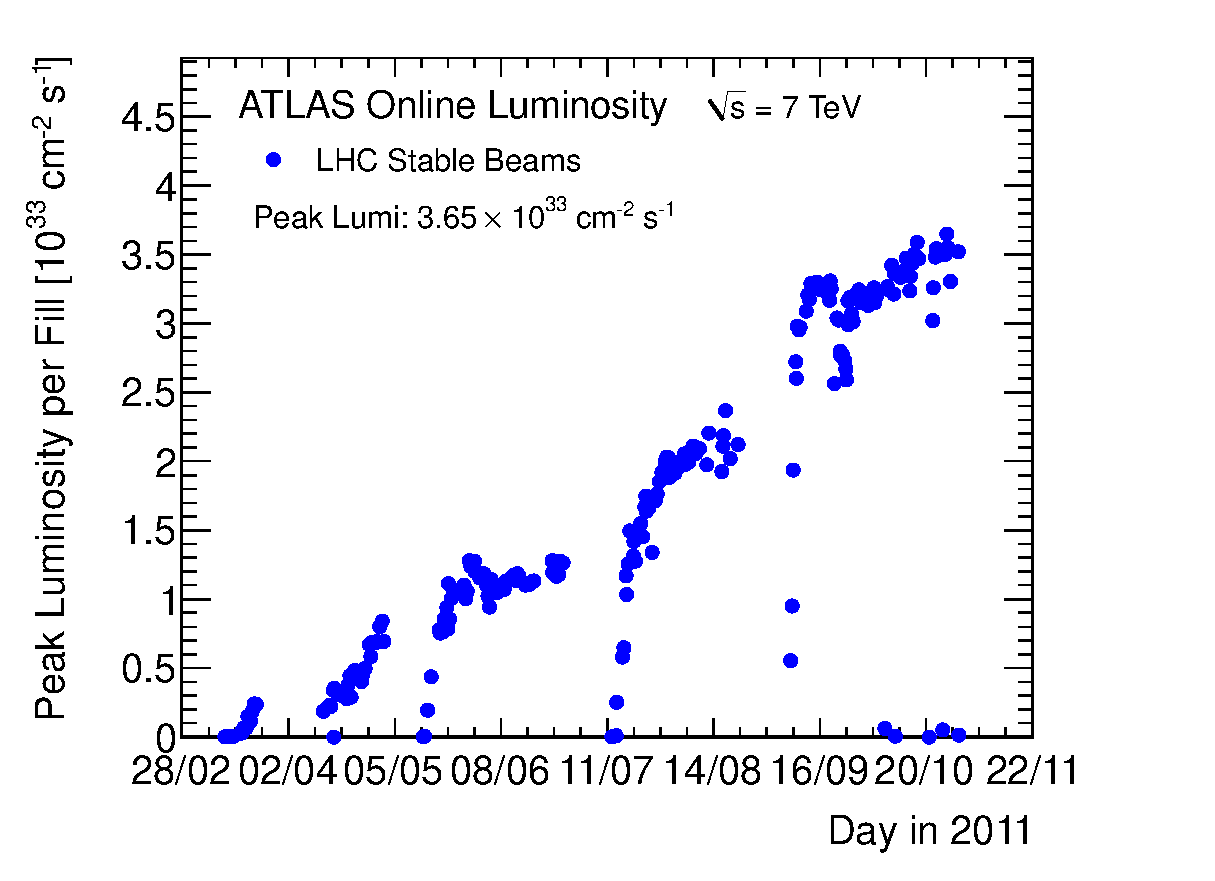
\includegraphics[width=0.47\textwidth]{peakLumiByFill2011}
%        }
%	\subfigure[]{
%            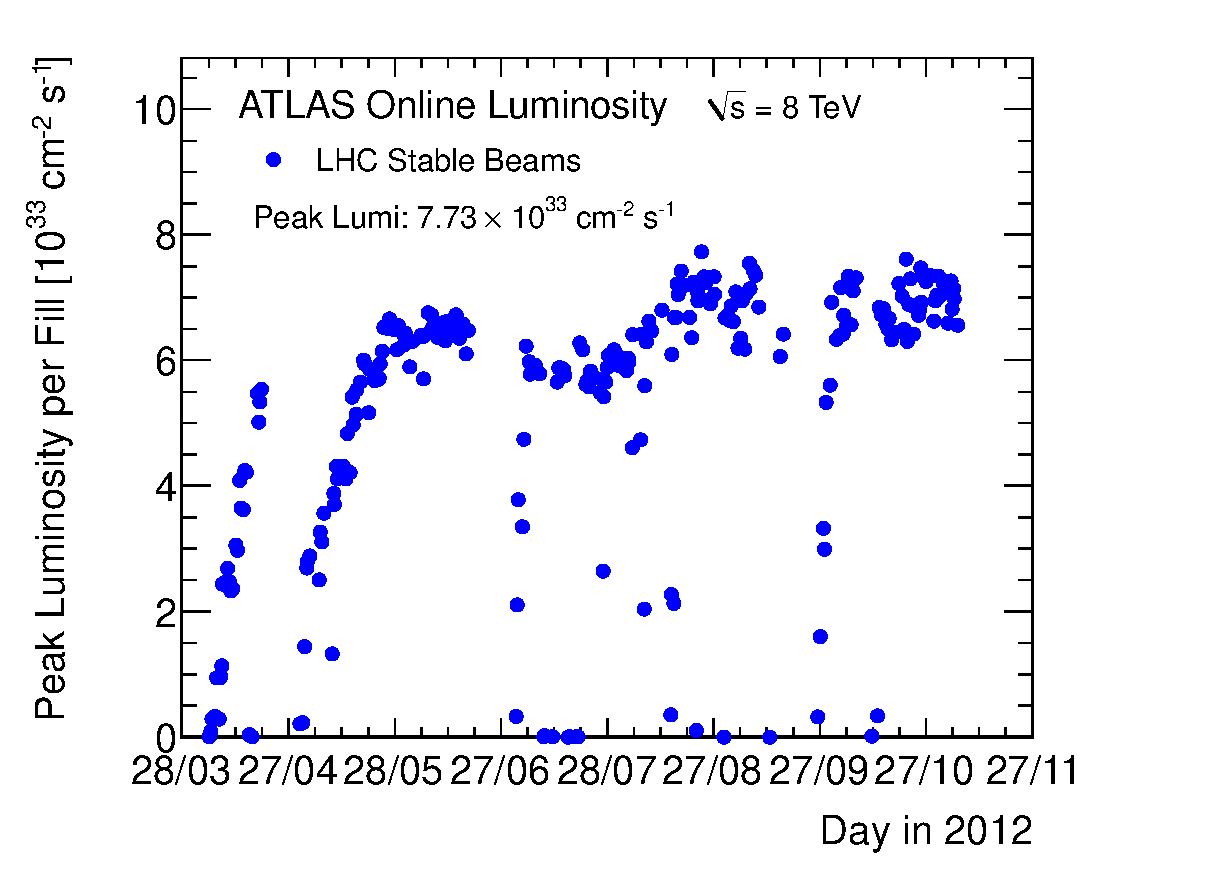
\includegraphics[width=0.47\textwidth]{peakLumiByFill2012}
%        }
\caption[Peak instantaneous luminosity delivered by the LHC per run as a function of time from
2010 to 2012.]{Peak instantaneous luminosity delivered by the LHC per run as a function of time from
2010 to 2012. Figure from~\cite{atlaslumipublic}.}
\label{fig:lhc-inst-lumi}
\end{figure}

\begin{figure}[h]
\centering
	\subfigure[]{
            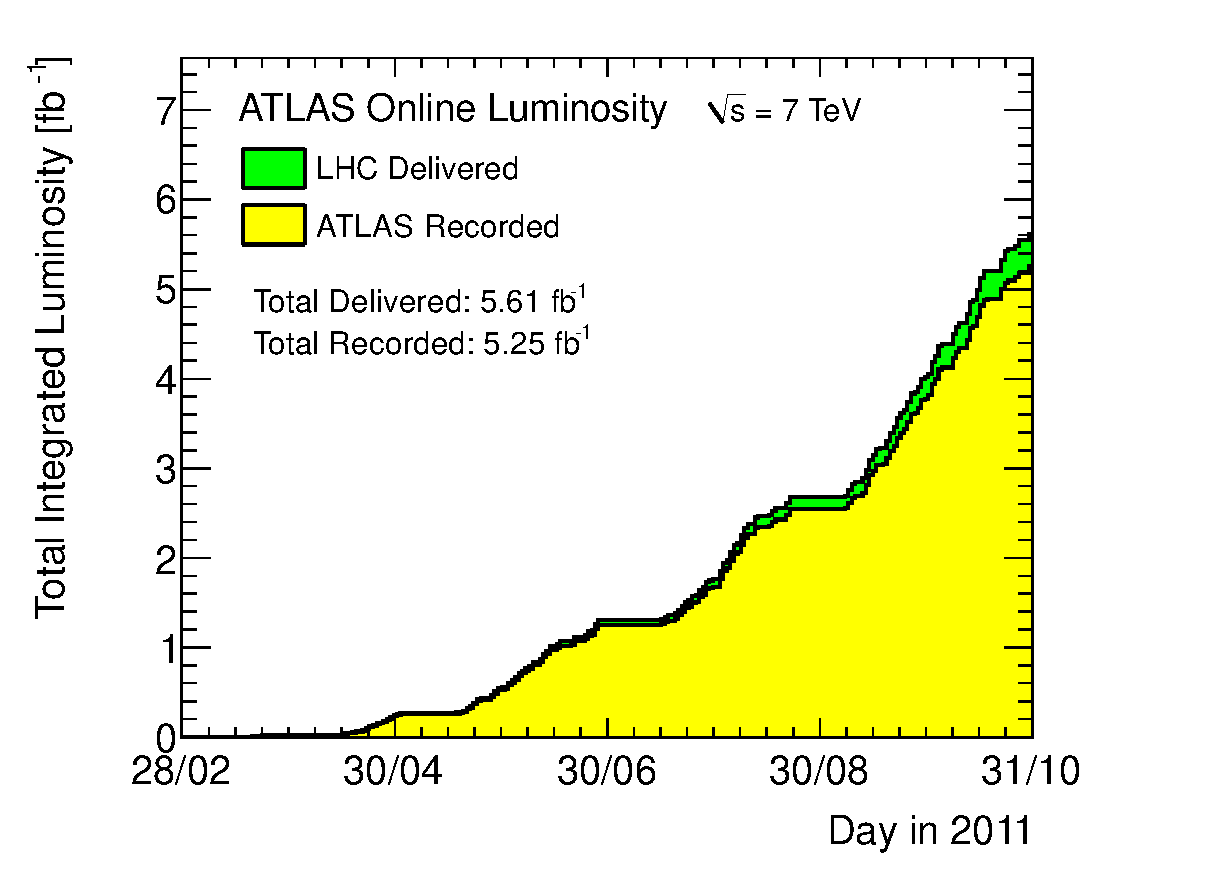
\includegraphics[width=0.47\textwidth]{sumLumiByDay2011}
        }
	\subfigure[]{
            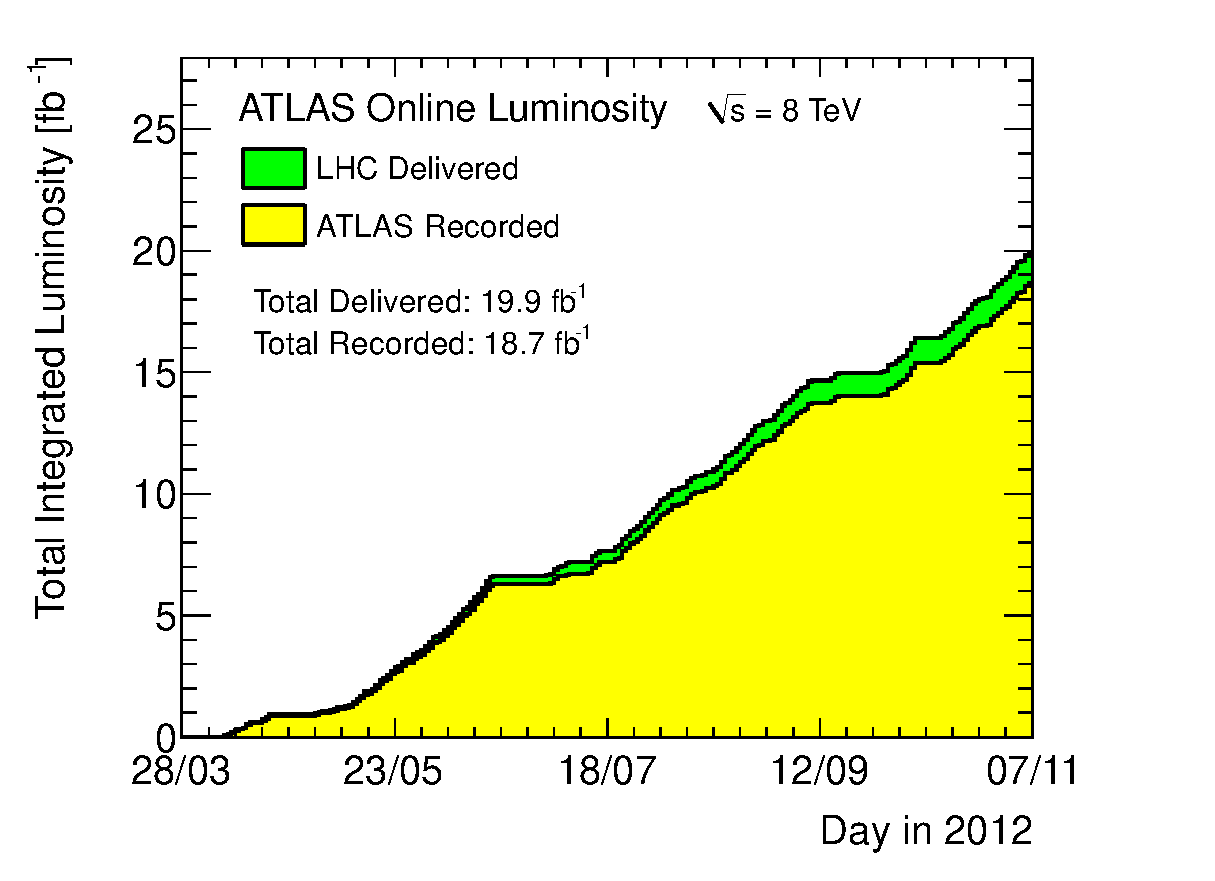
\includegraphics[width=0.47\textwidth]{sumLumiByDay2012}
        }
\caption[Cumulative integrated luminosity as a function of time in
2011 and 2012.]{Cumulative integrated luminosity as a function of time in (a)
2011 and (b) 2012. The totals for the two years are separate. 
Figures from~\cite{atlaslumipublic}.}
\label{fig:lhc-int-lumi}
\end{figure}

\fig{lhc-inst-lumi} shows the
instantaneous luminosity as measured by ATLAS as a function of time between 2010 and
2012. ~\fig{lhc-int-lumi} shows the cumulative integrated luminosity
delivered to ATLAS in 2011 and 2012.
Details of the LHC operational parameters in 2011 and 2012, together with the
nominal design values, are given in~\tab{lhc-params}.

% Say something about the luminosity here
% Say something about int lumi delivered to ATLAS


% Table comparing nominal parameters, 2011, 2012
% E.g. Inst. Lumi, Bunch spacing, # bunches / beam, # protons / bunch

\begin{table}[h]
\centering
\small
\setlength{\extrarowheight}{4pt}
\begin{tabular}{ l | c | c | c  }
\hline\hline
Parameter & Nominal & 2011 Operation & 2012 Operation \\
\hline
Proton Energy & 7 \tev\ & 3.5 \tev\ & 4 \tev \\
$N_{\rm{b}}$ & 1.15 $\times~10^{11}$ & 1.5 $\times~10^{11}$ & 1.6 $\times~10^{11}$  \\
$n_{\rm{b}}$ & 2808 & 1380 & 1380 \\
Bunch spacing (ns) & 25 & 50 & 50 \\
$\beta^{*}$ (m)  & 0.55 & 1.0 & 0.6 \\
$\epsilon_{n}$ (\micro m) & 3.75 & 1.9 - 2.3 & 1.7 - 3.0  \\
Peak $\mathcal{L}$ ($\rm{cm}^{-2}\rm{s}^{-1}$) & 1.0 $\times~10^{34}$  & 3.6 $\times~10^{33}$  & 7.7 $\times~10^{33}$ \\
\hline\hline
\end{tabular}
 \caption[LHC operational parameters.]{LHC operational parameters. A comparison is made of the nominal design
 parameters~\cite{Brüning:782076}, and those used in 2011 operation and in 2012
 operation~\cite{lhcstats}~\cite{Fournier:2012np}.}
        \label{table:lhc-params}
\end{table}
% https://lhc-statistics.web.cern.ch/LHC-Statistics/

\section{The ATLAS Detector}

ATLAS (A Toroidal LHC ApparatuS) is one of two general purpose particle-physics
detectors at the LHC, built to study both proton-proton and ion-ion
interactions. The high centre of mass energy and high luminosity of LHC proton-proton collisions
allows the study of physics at the \tev\ scale for the first time, as well as
precision measurements of the Standard Model. ATLAS has been designed to be
capable of a wide range of measurements, including (but by no means limited to):
high precision tests of QCD, electroweak interactions, and flavour physics; searching for and measuring
the properties of the Higgs Boson; searches for supersymmetery; measurements
of the properties of the top quark; searches for new vector bosons and searches
for extra-dimensions. 

The extremely high luminosity presents challenges which the detector has been
designed to overcome. At design luminosity, $10^9$ inelastic collisions occur
per second, which results in multiple interactions - up to
\PeakIntPerBunchCrossing\ in 2012 running - occurring simultaneously. The
detector has been designed to cope with these high `pile-up' conditions, as well
as be capable of operating in the high radiation environment arising from the
high luminosity. Many of the physics processes of interest occur at very small
rates with respect to extremely high QCD background rates. The detector must
therefore be capable of distinguishing processes of interest from the
background. 

To meet these challenges, ATLAS was defined with the following
criteria in mind:

\begin{itemize}
\item Fast, radiation-hard electronics and sensors.
\item High granularity to  cope with high particle fluxes and overlapping events.
\item Full azimuthal coverage to allow for missing transverse energy
measurement, and large acceptance in pseudo-rapidity.
\item Precision tracking to provide high charged particle momentum resolution
and reconstruction efficiency, and to allow observation of secondary vertices to
identify $b$-hadrons and $\tau$-leptons.
\item Precise electromagnetic calorimetry for electron and photon
identification.
\item Full-coverage hadronic calorimetry for accurate jet and missing transverse
energy measurements.
\item High muon identification efficiency, momentum resolution and charge determination over a wide range of
momentum.
\item Efficient triggering on low transverse-momentum objects with sufficient
background rejection.
\end{itemize}

The main performance goals are given in~\tab{perf-goals}.

\begin{table}[h!]
\centering
\small
\setlength{\extrarowheight}{4pt}
\begin{tabular}{ l | c | c | c  }
\hline\hline
Detector Component & Design Resolution & \multicolumn{2}{| c }{$\eta$
coverage} \\
& & Measurement & Trigger \\
\hline
Tracking & $\sigma_{\pt}/\pt = 0.05\% \, \pt \oplus 1\%$ & $\pm\,2.5$ & None \\
EM Calorimetry & $\sigma_{E}/E = 10\%/\sqrt{E} \oplus 0.7\%$ & $\pm\,3.2$ &
$\pm\,2.5$ \\
Hadronic Calorimetry & & & \\
\hspace{3mm} Barrel and End-Cap & $\sigma_{E}/E = 50\%/\sqrt{E} \oplus 3\%$ &
$\pm3.2$ & $\pm\, 3.2$ \\
\hspace{3mm} Forward & $\sigma_{E}/E = 100\%/\sqrt{E} \oplus 10\%$ & $3.1<|\eta|<4.9$ & $3.1<|\eta|<4.9$ \\
Muon Spectrometer & $\sigma_{\pt}/\pt = 10\%$ at \pt\ = 1 \tev\ & $\pm\, 2.7$ &
$\pm\, 2.4$ \\
\hline\hline
\end{tabular}
 \caption[Performance goals of the ATLAS detector.]{Performance goals of the ATLAS detector. Units of \pt\ and \E\ are
 \gev.}
	\label{table:perf-goals}

\end{table}

A cut-away view of the ATLAS detector~\cite{1748-0221-3-08-S08003} is shown in~\fig{atlas-det-1}. The detector consists
of an inner tracking detector, which is
surrounded by electromagnetic and hadronic calorimeters and finally a muon
spectrometer. The inner detector is immersed in a 2 T solenoidal field to allow
for momentum measurement. The muon spectrometer is also immersed in a magnetic
field, provided by an air-core toroid system  which generates strong
bending power over a large volume with a minimum of material, thus
minimising multiple-scattering effects. A three-level trigger system is used to select events to read out.
The various sub-systems are described in more detail in the following
sections. 

\begin{figure}[h]
\centering
\includegraphics[width=\textwidth]{{lhc-pho-1998-304}.jpg}
\caption[Cut-away view of the ATLAS detector.]{Cut-away view of the ATLAS detector~\cite{Jean-Luc:841458}. The
various detector sub-systems are labelled.}
\label{fig:atlas-det-1}
\end{figure}

\subsection{ATLAS Co-ordinate System}
ATLAS uses a right-handed coordinate system with an origin at the nominal
interaction point in the centre of the detector. The \z-axis points along the
beam-pipe, the \x-axis towards the centre of the LHC ring, and the \y-axis
upwards. Particle directions and detector element positions are generally
described by their azimuthal angle $\phi$ and their pseudorapidity $\eta$. The
azimuthal angle describes the angle in the \x-\y\ plane, with $\phi=0$ along the
\x\ axis, increasing clockwise around the beam-pipe.  The pseudorapidity $\eta$
is defined in terms of the polar angle $\theta$ (the angle in the $x-z$ plane)
as $\eta = - \ln\tan(\theta/2)$, and is an approximation to rapidity in the high
energy limit.  The radial co-ordinate \R\ measures the radial distance from the
interaction point. 

\subsection{Inner Detector}

The ATLAS Inner Detector (ID) is located closest to the beam pipe. It is a tracking
detector designed to provide hermetic coverage and robust pattern recognition, locate
interaction vertices, including displaced secondary vertices from long-lived
particles, and provide a precise measurement of the transverse momenta of charged
particles with a nominal \pt\ threshold of 0.5 GeV. It consists
of a silicon pixel detector (the \intro{Pixel Detector}), a silicon strip
detector (the \intro{Semiconductor
Tracker} or SCT) and a transition radiation tracker (the TRT), located within a
2 T magnetic field provided by a solenoidal superconducting magnet.

\begin{figure}[h]
\centering
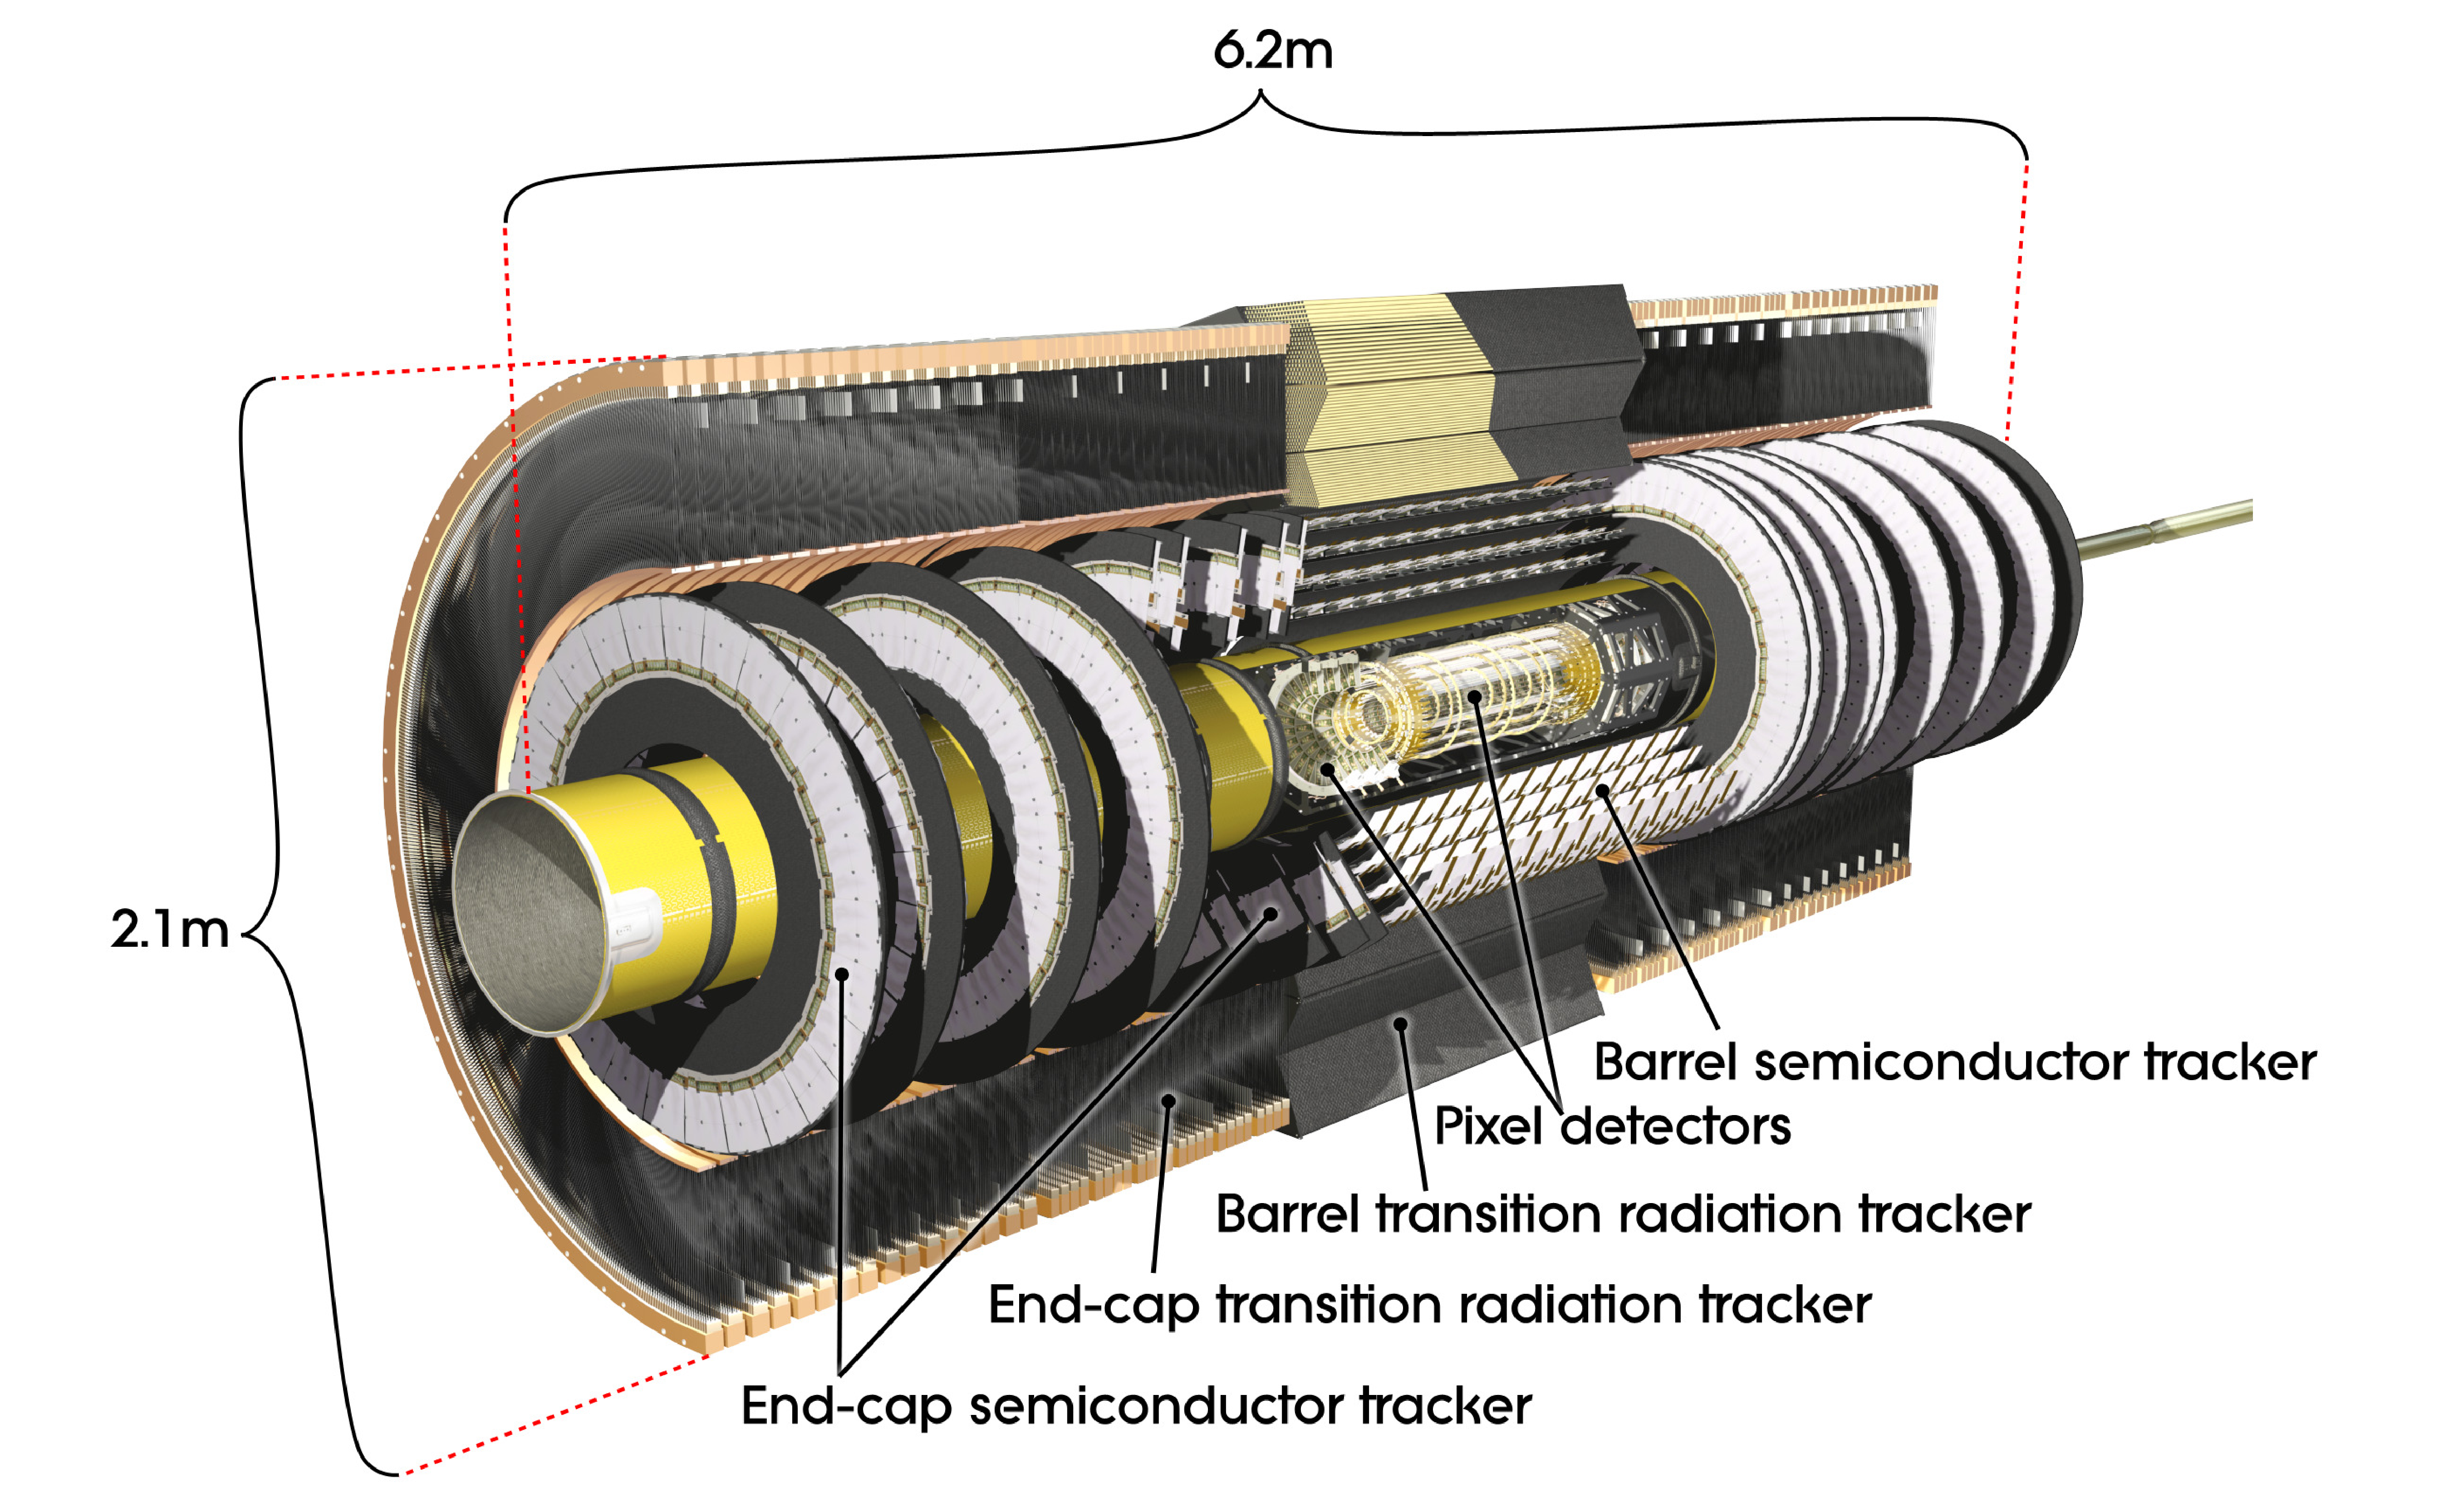
\includegraphics[width=\textwidth]{ID_newTRT_d3}
\caption[Cut-away view of the Inner Detector.]{Cut-away view of the Inner Detector, taken from~\cite{Aad:1125884}.}
\label{fig:id-1}
\end{figure}

A cut-away diagram of the Inner Detector is shown in \fig{id-1}. The detector
is cylindrical in shape, extending 3512 mm either side of the interaction point
in the \z\ direction with a radius of 1150 mm. The subdetectors all consist of
concentric cylindrical layers surrounding the beam pipe, referred to as
`barrels', with disks referred to as `end caps' covering each end of the
barrels. A plan view of a quarter of the Inner Detector is shown
in~\fig{id-plan}. The Pixel and SCT detectors provide coverage for $|\eta|<2.5$,
with the TRT enhancing pattern recognition and track momentum resolution for
$|\eta|<2.0$

\begin{figure}[h]
\centering
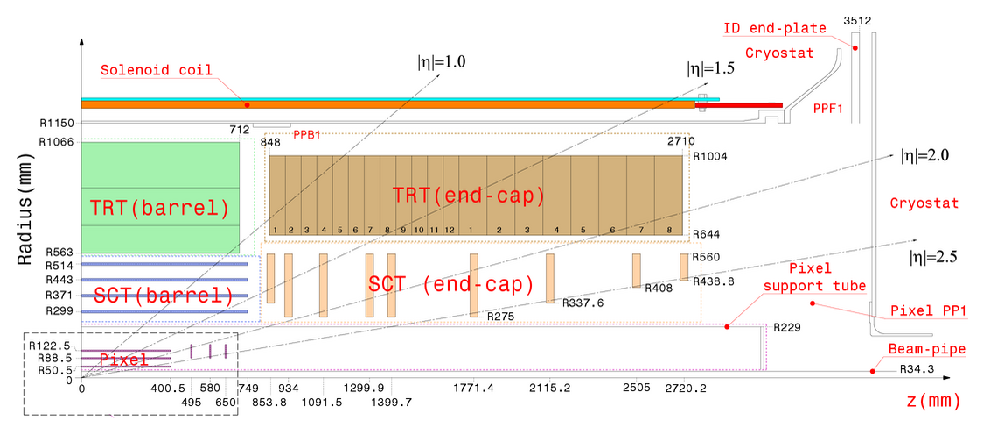
\includegraphics[width=\textwidth]{FigID26-mod-011107_crop}
\caption[Plan view of a quarter section of the Inner Detector showing the
positions and pseudo-rapidity coverage of the various subdetectors.]{Plan view of a quarter section of the Inner Detector showing the
positions and pseudo-rapidity coverage of the various subdetectors. Figure taken from~\cite{Aad:1125884}.}
\label{fig:id-plan}
\end{figure}

\subsubsection{Pixel Detector}

The pixel detector is the detector component closest to the beam. It is formed
of layers of silicon semiconducting pixels, and is designed to have a very
high granularity for resolving primary and secondary interaction vertices. There
are three barrel layers closed by an endcap consisting of three disks at each
end. The barrels are numbered from 0 to 2. The closest layer to the beam
pipe, termed the \b-layer (due to its important role in detecting secondary
vertices for \b\ physics), is
positioned at a radius of 50.5 mm. Due to the high radiation dose that it will
receive at this position, it will need to be replaced after three years of operation at design luminosity.

% Pixels in the region of the front end chips on a module are 50x600 um^2
The detector layers are formed of sensor modules, of which there are 1744 in
total. Each module consists of a 250 \micro m thick
silicon sensor consisting of 46,080 active pixels with nominal dimensions of
$50\times400~\mu \rm{m}^{2}$. In total
there are approximately $80.4\times 10^{6}$ readout channels.

Particles with \modetalt{2.0} will traverse three layers of the detector; in most case
producing three space-points. The intrinsic accuracy of the position
measurement is 10 \micro m in $(\rm{R}-\phi)$ and 155 \micro m in \z\ in the
barrel layers and 10 \micro m in $(\rm{R}-\phi)$ and 155 \micro m in $\phi$ in
the endcaps.

\subsubsection{Semiconductor Tracker (SCT)}

\label{sec:Detector-SCT}

The SCT is a silicon strip detector, consisting of four barrel layers and two end-caps
consisting of nine disks each. The barrel layers consist of 2112 separate modules and
extend from a radius of 299 mm from the beam line at the innermost layer to a
radius of 514 mm at the outermost. The layers are numbered from 3 to 6. Each
endcap consists of 988 modules, arranged in such a way that a particle must pass
through four layers of the detector.

%SCT modules are made from two pairs of single sided p-in-n silicon chips biased
SCT modules are made from two layers of single sided p-in-n silicon chips biased
at 150V (this voltage will increase as the detector become radiation damaged). 
Charged particles passing through the depletion region at the centre of
the junction produce electron hole pairs, which are swept apart by the bias
voltage. The electrons are then collected on the top of the chip, producing a
signal which can be read out. A photo of an SCT barrel module is shown
in~\fig{sct-barrel-module}.

Each side of the module consists of 768 strips of length 6.4~cm,
with a pitch of 80 \micro m for barrel modules, and an average pitch of 80
\micro m for endcap modules. The strips on one layer
of the module run parallel to the
beam axis on the barrel, and along the \R\ direction on the endcap. The other
layer is placed at a stereo angle of 40~mrad to form a two-sided module. 
%give resolution in the \z\ (\R\ co-ordinate on the barrel (endcaps). 
In total
there are approximately $6.3 \times 10^{6}$ readout channels.

% From http://atlas.web.cern.ch/Atlas/GROUPS/INNER_DETECTOR/SCT/gallery/barrel_modules/barrelmodule.jpg
% but could cite detector paper if need be
\begin{figure}[h]
\centering
\includegraphics[width=0.8\textwidth]{{SCTbarrelmodule}.jpg}
\caption[Photograph of an SCT barrel module.]
{Photograph of an SCT barrel module. Figure
from~\cite{1748-0221-3-08-S08003}}
\label{fig:sct-barrel-module}
\end{figure}

%Each pair of chips is wire-bonded together and two
%pairs 
 The readout is of a binary form, with a charge collection threshold of 1
fC (chosen to maximise efficiency and minimise noise). To form a space-point, a
coincidence of hits on either side of the module is required. The stereo
angle gives the ability to determine where along the strip the hit occurred,
giving resolution in \z\ (\R) in the barrels (endcaps). A small angle is used to
prevent ambiguities in the presence of multiple nearby hits. The spatial
resolution of the detector is 17~\micro m in ($\rm{R}-\phi$) and 580~\micro m in
\z\ (\R) in the barrel (endcaps).

\subsubsection{Transition Radiation Tracker (TRT)}
\label{sec:Detector-TRT}

The Transition Radiation Tracker is a straw drift tube tracker, with additional
particle identification capabilities from transition radiation. It consists of
modules formed from bundles of 4 mm diameter straws, filled with
$\rm{XeCO_{2}O_{2}}$ gas. A tungsten wire of 30 \micro m diameter runs down
the centre of the tube to collect charge. In the barrel the straws run parallel
with the beam axis and are 144 cm long. The wires are electrically divided into two halves at
\modetaeq{0} and read out at either end (this subdivision leads to an
inefficiency along a length of approximately 2 cm at the centre of the TRT). In
the endcaps the straws are 37 cm long and run radially. In total there are
351,000 readout channels.

% Number of hits - resolution - advantages of continuos tracking
All charged tracks with \ptgt{0.5} and \modetalt{2.0} will traverse at least 36
straws, except in the barrel to endcap transition region (\modetabetween{0.8}{1.0})
where only 22 straws will be traversed. The ($R-\phi$) resolution is 130 \micro
m. Despite the low resolution compared to the silicon trackers, and the lack of
a measurement in the \z\ direction, the hits in the TRT contribute significantly
to the pattern recognition and momentum resolution due to the large number of
measurements and longer measured track length.

% TR
The barrel straws are embedded in a matrix of 19 \micro m diameter polypropylene
fibres, and the endcap disk layers are sandwiched between 15 \micro m
polypropylene foils. When charged particles cross the boundary between the straw
and the fibre they emit
transition radiation photons. These photons are then absorbed by the Xenon gas
mixture, and produce much larger signals than minimum-ionising
charged particles. The energy of the transition radiation photons depends
heavily on particle type, and is approximately 200 keV for a 20 GeV electron and
1 keV for a 20 GeV pion. This difference can be exploited for particle
identification, by counting the number of hits over a higher threshold.
Electrons with \ptgt{2} typically produce 7 - 10 high threshold hits, whereas
pions and other charged particles will produce far fewer.

\subsection{Calorimetry}

The ATLAS
calorimeter systems sit outside the inner detector and its magnetic field. 
The purpose of the calorimeter is to measure the energy and
position of particles. A particle entering the calorimeter produces a
`shower' of secondary particles; the energy of this shower is then measured.
ATLAS uses sampling calorimeters, in which different materials, sandwiched
together in layers, are used to initiate the shower development (absorption) and
to measure the energy of its constituents. This
allows for a more compact design and hence better shower containment. Position
measurement is obtained by segmenting the calorimeter in the \z\ and $\phi$
directions.

Different absorbers are required depending on whether the particle interacts
via the electromagnetic or the strong force, and the properties of the showers that develop
are different. The ATLAS calorimeters are divided into two distinct subsystems,
the \emag\ calorimeter and the Hadronic calorimeter. An electromagnetic
shower consists of electrons and photons, and is normally fully contained in the
calorimeter; thus it can be fully detected. Hadronic showers involve many more
particles types, including neutrons, muons, and neutrinos which escape detection, and tend
to be longer and wider, often spilling out of the calorimeter. The full energy
of the shower is thus not fully detected, and so a calibration of the energy
response is required. It is important for the calorimeter to provide good
containment for electromagnetic and hadronic showers, not only for the purposes
of energy measurement, but also to allow a good missing transverse energy
requirement, and to prevent punch-through into the muon system.

\begin{figure}[h]
\centering
\includegraphics[width=0.9\textwidth]{{0803015_01}.jpg}
\caption[Cut-away view of the ATLAS calorimeter system.]{Cut-away view of the ATLAS calorimeter system. Image taken
from~\cite{1748-0221-3-08-S08003}.}
\label{fig:calo-cutaway}
\end{figure}

A cutaway view showing the location of the various calorimeter elements is shown
in~\fig{calo-cutaway}. The calorimeters cover the range \modetalt{4.9}. Over the
$\eta$ range of the inner-detector, the \emag\ calorimeter gives fine
granularity to allow precise measurement of electrons and photons. The hadronic
calorimeter is more coarsely segmented, but is sufficient to meet the
requirements of jet and missing transverse energy measurement.

\subsubsection{Electromagnetic Calorimeters}

The \emag\ (EM) calorimeter 
(also referred to as the \intro{LAr}) 
uses liquid
argon as the active detector material, and lead as an absorber. 
%Incident
%particles ionise atoms in the lead absorber, creating an electromagnetic shower.
Charged particles in the shower ionise the liquid argon, where the electrons
drift to copper electrodes in the presence of an electric field.

The LAr consists of two half barrels extending to \modetalt{1.475} (with
a 4~mm gap at \z\ = 0), and two coaxial wheels on each side (named the
\intro{EMEC}, the first covering
\modetabetween{1.375}{2.5} and the second covering \modetabetween{2.5}{3.2}.
Additional material needed to instrument and cool the detector creates a `crack'
region at \modetabetween{1.375}{1.52}, where the energy resolution is
significantly degraded.

The barrel calorimeter has an accordion structure in order to avoid azimuthal
cracks and to provide full $\phi$ symmetry, as shown in~\fig{lar-diagram}. The
accordion structure is made of the lead absorber, with the liquid argon filling
the 2.11 mm gaps between the absorbers. The barrel of the LAr calorimeter is
divided into three layers, with different cell granularity. The first layer is
divided into cells of \deltaetadeltaphi{0.0031}{0.098}. The fine granularity in
$\eta$ of this layer is used to determine the pseudo-rapidity of the particle,
and for measurements of the shower shape, an important input to particle
identification. The second layer has cell size \deltaetadeltaphi{0.0245}{0.025}
and contains the largest energy fraction of the shower, measuring approximately
16 radiation lengths. The third layer, with cell size
\deltaetadeltaphi{0.0245}{0.05}, collects the tail of the shower. The first
wheel of the LAr calorimeter is also segmented into three layers with the same
granularity as the barrel. The second wheel has a coarser granularity that
varies as a function of pseudorapidity. A liquid argon pre-sampler exists for
\modetalt{1.8} to correct for energy lost by incident particles traversing
material before the calorimeters, and to aid with discriminating between
$\pizero \to \gamma \gamma$ decays and prompt photons.

%The liquid argon has to be maintained at a temperature of 88 K.

\begin{figure}[h]
\centering
\includegraphics[width=0.8\textwidth]{lar-diagram}
\caption[Diagram of the ATLAS liquid argon calorimeter, showing the accordion
structure and the different granularity in the different layers.]{Diagram of the ATLAS liquid argon calorimeter, showing the accordion
structure and the different granularity in the different layers. Diagram taken
from~\cite{1748-0221-3-08-S08003}.}
\label{fig:lar-diagram}
\end{figure}

\subsubsection{Hadronic Calorimeters}

The hadronic calorimeter consists of a plastic scintillator tile calorimeter 
(referred to as the \intro{tile} calorimeter) covering \modetalt{1.7} and a liquid
argon endcap calorimeter (referred to as the \intro{HEC}) covering
\modetabetween{1.5}{3.2}. 

The tile calorimeter consists of a 5.8 m long barrel covering
\modetalt{0.8} and two 2.6~m long extended barrels covering
\modetabetween{0.8}{1.7}.
It is located immediately behind the EM calorimeter, extending from a radius of
2.28 m~to a radius of 4.25~m. The active material consists of 3~mm thick layers of the plastic scintillator 
placed perpendicular to the beam direction, sandwiched between steel absorbers.
The scintillators are connected at each end to
readout photomultiplier tubes by wavelength-shifting fibres. The fibres are grouped
together to form readout cells, giving projective towers in $\eta$. There are
three layers of cells, with a granularity of \deltaetadeltaphi{0.1}{0.1} in the
first two layers, and \deltaetadeltaphi{0.1}{0.2} in the third.

The HEC consists of two wheels per endcap, HEC1 and HEC2, located directly
behind the EMEC and sharing the same cryostat. Each wheel has two layers of
cells. The HEC covers \modetabetween{1.5}{3.2} and so overlaps with the tile
calorimeter on one side and the FCAL on the other, thus avoiding cracks in the
transition regions. HEC1 (HEC2) is built from 25 mm (50 mm) copper plate
absorbers interleaved with 8.5 mm gaps containing liquid argon. The liquid
argon gaps are split into four drift spaces of roughly 1.8 mm by three
electrodes. This is to avoid ion build-up due to the higher particles fluxes
and energies in the forward region, and also allows a lower high voltage than a single
electrode design.

\subsection{Forward Calorimeter}

The forward calorimeter ({\it FCAL}) covers \modetabetween{3.1}{4.9}. To reduce the
neutron flux, the FCAL begins 1.2 m away from the EM calorimeter
front face. Due to the high particle fluxes and energies in the forward region,
the calorimeter must contain relatively long showers in the small volume allowed
by design constraints, and thus must be very dense. The FCAL is divided into
three compartments. The first, FCAL1, is designed for electromagnetic
measurements, and uses copper as an active material with liquid argon as a
passive material. The second two compartments, FCAL2 and FCAL3, are designed for hadronic
measurements, and use tungsten as a passive material, chosen for its high
density to provide containment and minimise the lateral spread of hadronic
showers. An additional copper alloy shielding plate is placed behind FCAL3 to
reduce background to the muon endcap system.

\subsection{Muon Spectrometer (MS)}

The muon spectrometer sits outside the calorimeter system, and is designed to
provide precision muon momentum measurements over a momentum range of 3~GeV to
3~TeV, as well as providing triggering on bunch crossings containing
muons. An overview of the MS is given in~\fig{muon-cutaway}. The system sits
inside a giant air coil toroidal magnet system, producing a magnetic field
orthogonal to the muon momentum to provide deflection of the
muons for momentum measurement. The use of an air coil reduces multiple
scattering which degrades the momentum resolution.

\begin{figure}[h]
\centering
\includegraphics[width=0.8\textwidth]{{ms_cutaway}.jpg}
\caption[Cut away view showing the various components of the ATLAS muon
spectrometer.]{Cut away view showing the various components of the ATLAS muon
spectrometer. Figure taken
from~\cite{1748-0221-3-08-S08003}.}
\label{fig:muon-cutaway}
\end{figure}

The system consists of Monitored Drift Tubes (MDT) and Cathode Strip Chambers
(CSC) to provide precision measurements in the bending ($R-z$) plane. The MDT
covers \modetalt{2.7} and consist of three layers. 
%The mechanical isolation of
%the sensor wire in each tube from it's neighbours give a reliable system design.
In the innermost layer, for \modetabetween{2.0}{2.7} the MDT is replaced by the
CSC due to the higher rates and higher backgrounds in this region. The CSC is a
multiwire proportional chamber, and so gives a higher granularity than the MDT
and is better able to cope with high rates and fluxes.

Resistive Plate Chambers (RPC) and Thin Gap Chambers (TGC) provide triggering
for \modetalt{2.4} and a measurement in the $x-y$ plane for \modetalt{2.7}. The
RPC covers \modetalt{1.05}, with the TGC covering \modetabetween{1.05}{2.7}. The
muon trigger has a time resolution of between 1.5 ns and 4 ns.

\section{Trigger}
\label{sec:detector-trigger}

ATLAS uses a three-level trigger system to identify when to read out the
detector and to reduce the event rate to a manageable level by identifying
interesting events. The collision rate of approximately 20 MHz has to be reduced
to a rate of between 200 and 1000 Hz for offline reconstruction, storage and analysis.
An overview of the ATLAS trigger system is shown in~\fig{trigger_overview}. 

The
first level, L1, uses fast custom electronics to identify the presence of signals from a hard scattering such as
high \pt\ electrons, muons or jets, or a large amount or missing transverse
energy. The L1 trigger has a maximum latency of 2.5 \micro s, and must reduce
the rate to approximately 60 kHz (the design L1 rate was 75 kHz, however
significant detector dead-time has been observed above 65 kHz). To meet this
tight time constraint, only low-granularity signals from the calorimeters and dedicated muon trigger
chambers are used. The L1 trigger also identifies `Regions of Interest' (RoI)
surrounding the signature that caused the trigger to be fired, for use in later
levels of the trigger.

The second (L2) and third level (the \intro{Event Filter} or EF) trigger are software based, and are collectively known as the
`High Level Trigger' (HLT). At each level, the decision of the previous level is
refined by using more detector information and allowing a longer time for the
decision to be made and thus more complicated algorithms to be run, as well as
tightening the selection requirements to further reduce the rate. At L2 the full
readout from the RoIs identified at L1 is available. L2 uses dedicated
algorithms to return a decision based on the RoI information within 100 ms. The
EF has access to the full event readout, though typically only information
inside or just outside the RoI is used. The EF algorithms are based on the
offline object reconstruction algorithms, and may take up to 1~s to make
a decision.

The trigger is organised into `chains' with a L1 trigger seeding a chain of
algorithms in the HLT. Each chain is responsible for selecting a specific
trigger signature. The `trigger menu' is the collection of chains used to select
data during a run. It typically consists of about 200 primary chains for selecting data
for physics analysis and about 300 supporting chains for selecting data for
background and performance studies. The design of the trigger menu involves
balancing between the sensitivity for physics analysis resulting from the
trigger, and the need to reduce the rate to a level dictated by the available
resources for reconstruction and storage. The offline computing processing power
limits the EF trigger rate to about 400 Hz. The trigger menu had to evolve
throughout 2011 and 2012 to meet challenges posed by the constant increase in
instantaneous luminosity, and the increase of pileup to almost double the design
value. The measurements described in this analysis use single electron and muon
triggers. These triggers account for the largest slice of the trigger bandwidth,
with rates of approximately 50 Hz each. They are described in more detail
in Sections~\ref{sec:reco-el-triggers} and \ref{sec:reco-mu-triggers}.

\begin{figure}[h]
\centering
\includegraphics[width=0.8\textwidth]{trigger_overview}
\caption[An overview of the ATLAS trigger and DAQ system.]{An overview of the ATLAS trigger and DAQ system. The design and 2012
typical trigger rates at each level are shown on the left, and the design and
2012 typical output bandwidths are shown on the right. Figure taken
from~\cite{Petersen:1491585}.}
\label{fig:trigger_overview}
\end{figure}

\section{Detector Simulation}

Simulation of the detector response to various physics processes is a vital
ingredient to physics analysis. It is important for understanding and
calibrating the detector response to different signatures, for estimation of
acceptances and efficiencies, and also to be able to compare experimental
results with theoretical models. A custom detector simulator, which uses the
\geant~\cite{Agostinelli2003250} toolkit, is used to simulate interactions
between particles and matter in the ATLAS detector. It takes as input the output
of Monte-Carlo generators as described in~\sec{Theory-MC} in HepMC format, with all
particles with a lifetime less than $c \tau > 10$ mm decayed by the generator.
The simulator then propagates the particles through the ATLAS detector, using
\geant\ to simulate their interaction with the material of the detector. 

The response of the detector components to the particles produced is also
simulated, and simulated output signals are produced in the same format as the
real detector output. These are then reconstructed in the same way as for real
data (described in~\chap{Reconstruction}). To simulate the effect of pileup,
minimum bias events generated with the \pythia generator are overlaid with the
hard event.

\section{Luminosity Measurement}

An accurate measurement of the delivered luminosity is an essential ingredient
to any physics analysis, for example to enable the measurement of a \cx\ or to
allow the correct normalisation of simulated backgrounds. The instantaneous
luminosity can be expressed as:
\begin{equation}
\mathcal{L} = \frac{ \mu n_{b} f_{r} }{ \sigma{inelastic} }
\label{eqn:lumi-meas-1}
\end{equation}
where $\mu$ is the number of interactions per bunch crossing, $n_{b}$ is the
number of colliding bunch pairs and $\sigma{inelastic} $ is the inelastic \cx. The
instantaneous luminosity is measured during data taking by measuring the
observed interaction rate per bunch crossing $\mu_{vis}$. \eqn{lumi-meas-1} can
be rewritten in term of this quantity:
\begin{equation}
\mathcal{L} = \frac{ \mu_{vis} n_{b} f_{r} }{ \sigma{vis} }
\label{eqn:lumi-meas-2}
\end{equation}
where $\sigmaVis =\epsilon \sigma_{inelastic}$ is the total inelastic \cx\
multiplied by the efficiency of the method used to measure $\mu_{vis}$. The
parameters $\mu_{b}$ and $f_{r}$ are known machine parameters, and so a
measurement of $\mu_{vis}$ gives a measurement of the relative luminosity; this
must be calibrated by measuring $\sigma_{vis}$ in order to give an absolute
luminosity measurement.

Two primary detectors are used for the measurement of \muVis: LUCID and the BCM.
LUCID is specifically designed for measuring the luminosity for ATLAS, and is a
Cerenkov detector consisting of sixteen aluminium tubes filled with
$C_{4}F_{10}$ gas surrounding the beampipe each side of the interaction point
at a distance of 17 m. The Cerenkov photons are reflected down the tubes to
photomultipliers (PMTs); if one of the tube's PMTs records a signal over
threshold the tube records a `hit' for that event. LUCID receives signals
directly from the LHC clock allowing it to record event rates separately for
each bunch crossing, and is separate from the main ATLAS DAQ enabling luminosity
measurement even when the detector is not in data-taking mode. The BCM~\cite{1748-0221-3-02-P02004} (Beam
Conditions Monitor) primary function is to measure beam-induced backgrounds and
issue a beam-abort request in case of dangerous levels of background that would
be damaging to ATLAS. It consists of four diamond sensors located on each side
of the interaction point at a distance of 1.8 m; diamond sensors are chosen for
their radiation hardness and fast readout.

The calibration of \sigmaVis\ is done using dedicated \intro{van Der Meer (vdM)
scans}, where the absolute luminosity is measured directly from machine
parameters. The delivered luminosity can be written ad
\begin{equation}
\mathcal{L} = \frac{ n_{b} f_{r} n_{1} n_{2}}{ 2 \pi \Espilon_{x} \Epsilon{y} }
\label{eqn:lumi-meas-3}
\end{equation}
where $n_{1},n_{2}$ are the bunch charges in each beam, and
$\Epsilon_{x},\Epsilon_{y}$ are the vertical and horizontal width of the beam. In
a vdM scan, the beams are separated in steps of known distance, and the change
in event rates measured, giving a direct measurement of
$\Epsilon_{x},\Epsilon_{y}$. The bunch charge product is measured by two DC
current transformers, which have high accuracy but are unable to resolve
individual bunch charges, and two fast beam current transformers (FBCT) which
have lower accuracy but are able to resolve each
bunch~\cite{lhc-bunch-currents}. By
combining these measurements a direct measurement of the luminosity is made. By
comparing the peak luminosity (when the beam separation is at a minimum) with
the peak interaction rate, and using Equations~\ref{eqn:lumi-meas-2}
and~\ref{eqn:lumi-meas-3} a measurement of $\sigma_{vis}$ is obtained, enabling
absolute normalisation of the luminosity.

The luminosity measurement is cross-checked using an independent measurement of
the luminosity using information from the ATLAS calorimeters. The PMT current
from the tile calorimeter and the total ionisation current in the liquid argon
of the FCal are related to the mean number of particles interaction in the
calorimeter, and so are sensitive to the luminosity. The stability of the
luminosity measurement over longer periods is cross-checked using the number of
\Z\ bosons observed in a given period of running. 

\section{Data Samples}

The measurements described in this thesis use data collected in 2011 and 2012,
and correspond to the full datasets collected by ATLAS in each of those two
years. The dataset is broken down into {\it runs}, continuous periods of
data-taking typically corresponding to one fill of the LHC. Each run is further
broken down into {\it luminosity blocks} consisting of roughly two or three
minutes-worth of data-taking. Runs are grouped together into {\it periods}, with
the accelerator, detector and trigger conditions being similar in each period.
The periods within each year are labelled A to M.

Luminosity blocks where there were problems with the detector (for example a HV
trip in the LAr) which would affect the reconstruction of electrons, muons, jets
or other physics objects are removed using a ``Good Runs List'' which records
which luminosity blocks have such defects. After removing these luminosity
blocks the integrated luminosity of 2011 dataset is \LumiPassGRLTwentyEleven\
and the integrated luminosity of the 2012 dataset is
\LumiPassGRLTwentyTwelve\ifb. The uncertainty on the luminosity measurement is
\LumiUncTwentyEleven\ifb~\cite{ATLAS-CONF-2011-116,Aad:2011dr} for 2011 data and
\LumiUncTwentyTwelve for 2012 data.

% Performace of the detector over these periods ?


\graphicspath{{Chapters/SCT/Figures/}}

\chapter{SCT Temperature Monitoring}
%\chapter{ATLAS Semiconductor Tracker Temperature Monitoring}
\label{chap:SCT}

\section{Introduction}

In order to mitigate the effects of radiation damage and to prevent damage
caused by excessive heat, it is important to keep the SCT modules cool,
maintaining the silicon sensors at temperatures of approximately $-7^{\circ}$C.
The SCT and Pixel sub-detectors use a common evaporative cooling system to
remove heat from their modules. Monitoring of the module temperature is
important to ensure that the cooling system is functioning as designed, and that
the modules remain coupled to the cooling structures.  Additionally, monitoring
of the temperature difference between the front and the back of barrel modules
provides a check of the mechanical integrity of the modules. This chapter
describes tools developed to monitor variables associated with the temperatures
of SCT modules, and presents results for thirty-two months of operation between
January 2010 and October 2012.

%An overview These are described in this section, along with results for
%twenty-two months of operation between January 2010 and October 2012. 

%An
%overview of the Inner-Detector cooling system is given in
%Section~\ref{sec:SCT-CoolingDesc}.
%An overview of the
%Semiconductor Tracker (SCT) was given in
%Section~\ref{sec:Detector-SCT}. 

\subsection{Effects of Radiation Damage on Semiconductor detectors}

Given the LHC design luminosity of $10^{34}$ cm$^{-2}$s$^{-1}$, the inner layers
of the SCT are expected to receive a radiation dose of up to
$2\times10^{14}\;\rm{n_{eq}/cm}^2$~\cite{Ahmad200798} over the course of its
design lifetime of 10 years.  Exposure to such high radiation doses causes
damage to the silicon detectors. 

The primary method of radiation damage is interactions with irradiating
particles displacing nuclei from their lattice position, damaging the structure
of the material. Displaced nuclei can form stable defects in the material, which
change the effective doping. Exposure to radiation will cause an n-type
semi-conductor to become more p-type, and will eventually change the material
from n-type to p-type, in an effect known as \intro{type-inversion}.  The change
in effective doping has two effects: a loss of mobility of drifting electrons
and ions due to recombination, and an increase in the leakage current across the
p-n junction. This leads to lower charge collection efficiency and increased noise.
Charge collection efficiency can be maintained by increasing the displacement
voltage applied to the junction, though for sufficiently high radiation doses it
becomes impossible to fully deplete the sensors. It is therefore essential to
reduce the effects of radiation damage as much as possible.
 
%The effects of exposure to radiation have both an immediate and a prolonged
%effect. Immediate effects include the removal of donor nuclei from the
%lattices, and creation of acceptor like defects. Due to the complicated
%kinetics of these defects after the radiation, after type inversion has
%occurred an annealing effect occurs which initially reduces the number of
%acceptor-like defects, on a timescale of approximately two days, but on a
%longer term a `reverse annealing' occurs, increasing the number of acceptors.
%The rate of the reverse annealing effect is dependant on the temperate of the
%silicon. It is found that for temperatures of approximately -7$^{\circ}$C the
%reverse-annealing effect is effectively frozen out~\cite{Lindstrom2001308}.
%Since the reverse annealing occurs even after radiation, it is important to run
%the detector cooling at all times, not just when particle collisions are
%occurring.

It is found that for temperatures of approximately -7\dc\ the effects of
radiation damage are greatly reduced~\cite{Lindstrom2001308}, so it is important
to maintain the silicon at these low temperatures. After type-inversion occurs,
a process known as reverse-annealing occurs, whereby the radiation damage
continues to occur even after exposure to the radiation has ceased. After
type-inversion, it will therefore be necessary to run the detector cooling even
when there are no beams in the LHC.

The leakage current is induced by thermal creation of electron-hole pairs from
shallow donors arising from defects in the material, and increases the signal to
noise ratio of the sensor. The size of the leakage current is dependent on
the temperature of the sensor, and so reducing the temperature decreases the noise due to leakage
currents.

%\begin{equation}
%I_{\rm{leakage}} (T) \propto T^{2} \rm{e}^{-\frac{E_{g}}{2k_{B}T}}
%\end{equation}

\subsection{SCT Module Design}

\begin{figure}[h]
\centering
\centering
	\subfigure[]{
		\includegraphics[width=0.44\textwidth]{barrel_module_diagram}
	}
	\subfigure[]{
		\includegraphics[width=0.51\textwidth]{ec_module_diagram}
	}
\caption[Diagram of (a) an SCT barrel module and (b) an SCT endcap module.]
{Diagram of (a) an SCT barrel module and (b) an SCT endcap module, showing the
location of the different components. Figure
from~\cite{1748-0221-3-08-S08003}}
\label{fig:module-diagram}
\end{figure}

SCT modules consist of two layers of silicon sensors, bonded together at a small
stereo angle as described in~\sec{Detector-SCT}.~\fig{module-diagram} shows a
diagram of the layout of barrel and endcap modules. Barrel modules are
constructed by gluing the sensors either side of a graphite base-board which
provides the module's mechanical structure. The read-out chips are located on a
polyimide hybrid wrapped around the outside of the module. The HV is applied to
the sensors via the base board. Endcap modules are constructed in a similar
fashion, gluing the sensors either side of a base-board spine, with the hybrid
located at one end of the module. Heat from the sensors and from the read-out
electronics on the hybrid is conducted by the base-board to the cooling pipe,
which is connected at one edge of the module via a layer of thermal grease and
an aluminium cooling block.

\subsection{The Inner Detector Cooling System}
\label{sec:SCT-CoolingDesc}
%As described in the
%previous section, the SCT silicon detectors must be run
%at temperatures of around -7$^{\circ}$C in order to slow the rate of radiation
%damage and prolong their lifetime. 
%The Pixel silicon detectors must be held at
%0$~\circC$ for similar reasons~\cite{1748-0221-3-07-P07007}.
Each SCT module produces between 5.5W and 6W of heat when the ``High
Voltage (HV)'' biasing voltage is applied. This is expected
to increase to around 8W as the detector suffers the effects of radiation
damage and the bias voltage must be increased to compensate. 
An active cooling system based upon
evaporative cooling is used to remove this heat from the SCT modules
~\cite{1748-0221-3-07-P07003} and hold them at the low temperatures necessary to
mitigate the effects of radiation damage. The system is common to the SCT and
the Pixel detector. 

An evaporative cooling system was chosen over a mono-phase system as it has a
larger cooling capacity per unit volume due to utilisation of the latent heat of
vaporisation rather than a liquid's heat capacity. This allows the resulting
system to be smaller and with a lower mass, thus resulting in less material in
the inner-detector. Additionally, an evaporative system has
smaller temperature gradients along long cooling tubes, allowing for more
uniform module temperatures.

~\fig{evap-cooling} shows a schematic of the cooling system.  The system uses
the fluorocarbon refrigerant C$_3$F$_8$ as a cooling fluid, chosen since it is
stable against irradiation, non-flammable, non-toxic, electrically neutral, and
has the highest heat transfer coefficients of similar fluorocarbon
refrigerants. The cooling fluid is delivered at room temperature in saturated
liquid phase to capillaries located immediately before the detector structure.
The fluid expands through the capillaries and passes along the cooling pipe at
boiling point. The modules are coupled to the pipe by means of cooling blocks
and heat is absorbed from the modules by the passing fluid causing it to
evaporate. At the end of the cooling pipe a heater evaporates any residual
liquid and heats the vapour to above the cavern dew point to avoid condensation
in the return pipes.  The exhaust gas is piped to the ATLAS service cavern where
it is compressed and condensed, and then returned to the cooling loop.
Recuperative heat exchangers are used to transfer heat between the cold return
vapour and the warm inlet liquid, increasing the efficiency of the thermodynamic
cycle by decreasing the vapour quality\footnote{The \intro{vapour quality} of a
saturated fluid is the mass-fraction that is vapour.} of the fluid at the inlet to the cooling
structure. The temperature to which the modules are cooled depends on the
boiling pressure of the fluid, which is controlled by backpressure regulators
(BPR) located at the end of the return tubes.

\begin{figure}[h]
\centering
\centering
\includegraphics[width=0.6\textwidth]{{EvapCooling2}}
\caption[Schematic of the SCT evaporative cooling system.]
{Schematic of the SCT evaporative cooling system. Figure
from~\cite{Viehhauser:2006ix}}
\label{fig:evap-cooling}
\end{figure}


The cooling system consists of 204 independent cooling circuits or `loops', of
which 44 cool modules on the SCT barrels, 72 cool modules on the SCT endcaps and
the remaining 88 cool modules on the Pixel detector.

\section{Methodology}

The temperatures of SCT modules are monitored by thermistors mounted on the
module hybrids on the front side of the
module (the side furthest from the interaction point). Barrel modules have
an additional thermistor mounted on the back side of the module.  
The temperatures recorded by the module thermistors are read out by the ATLAS
\textit{PVSS} SCADA system. Every 12 hours the temperatures are written to an
Oracle database for offline analysis. In addition, whenever a module temperature
changes above a deadband of 0.4\dc, the new value is written to the
database.  

It is important to monitor the module temperatures only during periods of stable running, as
the temperatures will vary as the detector is cooled down or warmed up, or when
calibration work is in progress. Stable periods are
found by requiring that the number of cooling loops turned on is constant and
greater than zero. Stable periods are required to be at least 6 hours long, to
veto periods where the detector is being turned on and off, and stable periods
longer than 24 hours are broken down into 24 hour blocks.

For each module, a number of monitoring variables are calculated; these are
described below. The distributions of these variables are plotted for each of
the barrel layers and endcap disks. Modules which fall in the tails 
regions of the distributions are identified as `problem' modules. A list of
problem modules is maintained, and these modules are monitored. The monitoring plots are
produced automatically on a daily basis by scripts running on one of the SCT
monitoring computers and are made available as part of the `SCT
Calibration Monitoring' website at
\url{https://pc-sct-www01.cern.ch/CalibMonitor/} (ATLAS login required).

\section{Monitoring Variables}

\subsection{Front-Back Temperature Difference - \deltat }

The difference in temperature between the front and the back of a module
should be very small and any large temperature difference would indicate
defective thermal coupling between the two sides. This would suggest that the
front and the back of the module had lost mechanical integrity and were coming
apart from one another. It is therefore useful to monitor modules \deltat, the
front-back temperature difference, defined as:

\begin{equation}
 \Delta T = T_{\mathrm{front}} - T_{\mathrm{back}}
\end{equation}
where $T_{\mathrm{front}}$ and $T_{\mathrm{back}}$ are the temperatures recorded at the front and the back of the module respectively. 

%\begin{figure}[h]
%\centering
%\centering
%\includegraphics[width=\textwidth]{{20120922.0120-20120923.0120_delta_t_AllBarrels}.pdf}
%\caption[\deltat\ distribution for all SCT barrels averaged over the period 01:20
%22/9/2012 to 01:20 23/9/2012.]
%{\deltat\ distribution for all SCT barrels averaged over the period 01:20
%22/9/2012 to 01:20 23/9/2012. The distribution is fit to a Gaussian; the mean
%and width of the Gaussian is indicated on the plot.}
%\label{fig:dt_dist}
%\end{figure}

\begin{figure}[h]
	\centering
	\subfigure[]{
		\includegraphics[width=0.47\textwidth]{{20120922.0120-20120923.0120_delta_t_Barrel3}.pdf}
	}
	\subfigure[]{
		\includegraphics[width=0.47\textwidth]{{20120922.0120-20120923.0120_delta_t_Barrel4}.pdf}
	}
	\subfigure[]{
		\includegraphics[width=0.47\textwidth]{{20120922.0120-20120923.0120_delta_t_Barrel5}.pdf}
	}
	\subfigure[]{
		\includegraphics[width=0.47\textwidth]{{20120922.0120-20120923.0120_delta_t_Barrel6}.pdf}
	}
  \caption[\deltat\ distributions for the SCT Barrels for 01:20 22/9/2012 to 01:20 23/9/2012.]
  {\deltat\ distributions for the SCT Barrel 3 (a), Barrel 4 (b), Barrel
  5 (c) and Barrel 6 (d) for 01:20 22/9/2012 to 01:20 23/9/2012. The
  distributions are fitted to a Gaussian; the mean and width of the Gaussian is
  indicated on the plot.}
	\label{fig:dt_dist_barrels}
\end{figure}



For each period of stable operation the distribution of \deltat\ is plotted, for
all barrels together as well as for each barrel separately. Example plots for
01:20 22/9/2012 to 01:20 23/9/2012 are shown 
%in Figure~\ref{fig:dt_dist} (all barrels) and  
in~\fig{dt_dist_barrels} (separately for each barrel).
The distributions are fitted with a Gaussian and the mean and width of the
Gaussian are obtained. These are listed in Table~\ref{table:dt_thresh} for each
of the barrel layers, averaged over 5 months of data between 20/1/2010 and
20/6/2010.  

In order to identify modules with a high value of \deltat, a threshold of 5
times the width of the Gaussian is set, separately for each barrel. Modules with
a value of \deltat\ greater than this threshold are identified as `problem
modules'. Table~\ref{table:dt_num} gives the number and percentage of modules
with front-back temperature difference greater than the threshold at least five
times during the period 20/1/2010 to 19/6/2010, for each barrel layer. The width
of the distribution is greatest for Barrel 3, and so the thresholds for
identifying high \deltat\ modules is highest for this barrel. The width of the
distribution for Barrel 6 is the second widest, however the distribution is
observed to have large non-Gaussian tails, leading to a larger fraction of
problematic modules on Barrel 6 than other modules. This is attributed to the
fact that for Barrels 3, 4 and 5 only modules with $|\deltat | <
2^\circ$C measured on production were accepted, whereas for Barrel 6 this was
relaxed to $|\deltat| < 4^\circ$C~\cite{Viehhauser:2006ix}. 

The mean value of the \deltat\ distributions tend to be negative, implying that
on average the back side of the modules (the side facing into the carbon fibre
barrel) tends to be warmer than the front. This effect was also observed in tests
carried out on the modules reception at CERN in 2006~\cite{Viehhauser:2006ix},
and in tests carried out in 2008~\cite{Shaw:1229428}. Investigations suggested
that this bias is a property of the module itself, rather than an effect due to
the module's environment. A possible explanation is the way that the hybrid was
glued to the substrate, whereby the top wing of the hybrid was first glued to the front of the
module, then the bend made, then the bottom wing glued. It is possible that
following the bend the quality of the glue joint decreased, increasing thermal
impedance between the back of the hybrid and the base-board.

\begin{table}
\centering
\begin{tabular}{ l  c  c  c  c }
\hline\hline
Barrel & $\sqrt{\langle \sigma ^ 2 \rangle }$ & $5\sqrt{\langle \sigma ^ 2 \rangle }$ & $\chi ^2 $  / ndf & $\langle \Delta T_{\mathrm{mean}} \rangle$ \\
\hline
All barrels & 0.52 & 2.61 & 132.64 & -0.25\\
Barrel 3 & 0.64 & 3.21 & 19.44 & -0.36 \\
Barrel 4 & 0.39 & 1.96 & 8.22 & -0.21 \\
Barrel 5 & 0.48 & 2.38 & 36.06 & -0.23 \\
Barrel 6 & 0.60 & 3.02 & 59.06 & -0.26 \\
\hline\hline
\end{tabular}
 \caption{The width, goodness of fit and mean of the Gaussian fit to the
 \deltat\ distribution averaged over stable periods between 20/1/2010 and 20/6/2010.}
	\label{table:dt_thresh}

\end{table}

\begin{table}
\centering
 \begin{tabular}{  l  c  c }
\hline\hline
Component & \# Problem Modules & \% Modules Problematic \\
\hline
Barrel 3 & 1 & 0.3 \\
Barrel 4 & 1 & 0.2 \\
Barrel 5 & 7 & 1.2 \\
Barrel 6 & 17 & 2.5 \\
\hline\hline
\end{tabular}
\caption{Number and percentage of modules with $|$ \deltat$|$ greater than the
threshold for identifying problem modules at least 5 times during the period
20/1/2010 - 19/6/2010 for each barrel.}
\label{table:dt_num}
\end{table}

\subsection{Difference In Temperature To Local Average - \tdiff\ }

Modules with a bad thermal coupling to the cooling pipe can be identified by
looking for modules with a temperature significantly different to other modules
on the same cooling structure. The monitoring variable \tdiff\ is defined as:

\begin{equation}
T_{\mathrm{diff}}  = \bar T_{\mathrm{struct}} - T_{\mathrm{module}}
\end{equation}
where:
\begin{equation}
\bar T_{\mathrm{struct}} = \frac{\Sigma^N_1 T_{\mathrm{i}}}{N}
\end{equation}
is the average temperature of modules on the cooling structure. For the SCT
barrels a cooling structure is defined as a stave (consisting of two loops) and
for the endcaps it is defined as a single cooling loop. Any module warmer than its neighbours gives
a negative value of \tdiff, whilst modules cooler than their
neighbours give a positive value.

\begin{figure}
	\centering
	\subfigure[]{
		\includegraphics[width=0.47\textwidth]{{20120922.0120-20120923.0120_t_diff_AllBarrels}.pdf}
	}
	\subfigure[]{
		\includegraphics[width=0.47\textwidth]{{20120922.0120-20120923.0120_t_diff_EndcapA}.pdf}
	}
	\subfigure[]{
		\includegraphics[width=0.47\textwidth]{{20120922.0120-20120923.0120_t_diff_EndcapC}.pdf}
	}
	\caption{\tdiff\ distributions for the SCT barrel and endcaps for 01:20 22/9/2012 to 01:20 23/9/2012}
	\label{fig:tdiff_dist}
\end{figure}

Figure~\ref{fig:tdiff_dist} shows the distributions of \tdiff\ for the barrel
and for each of the endcaps for 01:20 22/9/2012 to 01:20 23/9/2012. As expected
the mean of the distribution is consistent with zero. Endcap C shows a large
tail to low \tdiff, indicating there are a large number of modules warmer than
other modules on their cooling loop. Examination of the distributions for each
disk suggest that this effect is observed on disks 1-5, but not on disks 6-9.
The cause of this effect is unknown.

\begin{table}[h]
 \centering
\begin{tabular}{ l  c  c  c }
\hline\hline
Barrel & $\sqrt{\langle \sigma ^ 2 \rangle }$ & $5\sqrt{\langle \sigma ^ 2 \rangle }$ & $\chi ^2$  / ndf\\
\hline
\textbf{All Barrels} & 0.81 & 4.03 & 48.82 \\
Barrel3 & 0.87 & 4.33 & 12.66 \\
Barrel4 & 0.71 & 3.56 & 13.88 \\
Barrel5 & 0.82 & 4.09 & 18.5 \\
Barrel6 & 0.77 & 3.84 & 35.44 \\
\hline
\textbf{EndcapA All Disks} & 1.31 & 6.53 & 28.68 \\
EndcapA Disk1 & 1.33 & 6.67 & 11.17 \\
EndcapA Disk2 & 1.38 & 6.89 & 14.93 \\
EndcapA Disk3 & 1.26 & 6.31 & 15.21 \\
EndcapA Disk4 & 1.28 & 6.42 & 11.04 \\
EndcapA Disk5 & 1.49 & 7.43 & 19.32 \\
EndcapA Disk6 & 1.45 & 7.27 & 15.54 \\
EndcapA Disk7 & 1.81 & 9.05 & 13.96 \\
EndcapA Disk8 & 1.39 & 6.95 & 10.05 \\
EndcapA Disk9 & 1.96 & 9.8 & 9.05 \\
\hline
\textbf{EndcapC All Disks} & 1.31 & 6.57 & 44.63 \\
EndcapC Disk1 & 1.24 & 6.21 & 17.52 \\
EndcapC Disk2 & 1.41 & 7.03 & 14.18 \\
EndcapC Disk3 & 1.26 & 6.28 & 19.22 \\
EndcapC Disk4 & 1.41 & 7.07 & 18.36 \\
EndcapC Disk5 & 1.19 & 5.96 & 19.22 \\
EndcapC Disk6 & 1.64 & 8.22 & 11.29 \\
EndcapC Disk7 & 1.25 & 6.27 & 11.17 \\
EndcapC Disk8 & 1.29 & 6.47 & 13.39 \\
EndcapC Disk9 & 1.72 & 8.58 & 9.38 \\
\hline\hline
\end{tabular}
\caption[The width of a Gaussian fit to the \tdiff\ distribution for each
stable period between 20/1/2010 and 20/6/2010.]
{The first column shows the width of a Gaussian fitted to the \tdiff\ distribution for each
stable period between 20/1/2010 and 20/6/2010. The threshold used for
identifying high \tdiff\ modules is set as 5 times this value; this is shown
in the second column. The third column shows the $\chi^2$ goodness of fit
parameter.}
\label{table:tdiff_thresh}
\end{table}

As with the \deltat\ monitoring variable, five times the average width of the
Gaussian fit is used as a threshold for identifying problem modules. The
threshold is set separately for each SCT barrel layer and endcap disk. The
thresholds are given in Table~\ref{table:tdiff_thresh}. The endcaps tend to have
much wider distributions than the barrels, indicating that the module
temperature is less uniform on endcap cooling loops. This is consistent with the
findings of the 2008 study~\cite{Shaw:1229428}. The number and percentage of modules with $|$
\tdiff$|$ greater than threshold at least 5 times during the period 20/1/2010 -
19/6/2010 is shown in Table~\ref{table:tdiff_num}.

\begin{table}
 \centering
\begin{tabular}{  l  c  c }
\hline\hline
Component & \# Problem Modules & \% Modules Problematic \\
\hline
Barrel 3 & 3 & 0.8 \\
Barrel 4 & 1 & 0.2 \\
Barrel 5 & 3 & 0.5 \\
Barrel 6 & 6 & 0.9 \\
Endcap A & 4 & 0.4 \\
Endcap C & 9 & 0.9 \\
\hline\hline
 \end{tabular}
\caption{Number and percentage of modules with $|$ \tdiff$|$ greater than the
threshold for identifying problem modules at least 5 times during the period
20/1/2010 - 19/6/2010 for each barrel and for each of the endcaps.}
\label{table:tdiff_num}
\end{table}

The majority of the modules above threshold had negative values of \tdiff,
indicating that they are warmer than their neighbours. This is generally caused
by the modules not being in complete contact with their cooling block. A small
number of modules had very large positive values of \tdiff, indicating that they
are cooler than their neighbours. This indicates a lower power dissipation
through the module which is either due to the module being disabled and thus not
receiving the high voltage current, or due to incorrect chip settings.

\section{Time Evolution of Monitoring Variables}

In order to track problematic modules, plots are produced each month showing the
problem modules and on which days they were problematic. An example of such a
plot is shown in Figure~\ref{fig:pm_april}. These plots are available on the
calibration monitoring website.

\subsection{Number of Problem Modules}

\begin{figure}
	\centering

	\subfigure{
		\includegraphics[width=\textwidth]{042010_Barrel5}
	}

	\caption{Problem modules on barrel 5 in April 2010.}
	\label{fig:pm_april}
\end{figure}
 
Of obvious concern is whether the number of problematic modules is increasing.
Figure~\ref{fig:num_pm} shows the number of problem modules above the problem
threshold on a given day as a function of time between 20/01/2010 to 16/10/2012
for the \deltat\ and \tdiff\ monitoring variables. For both monitoring
variables, there is no significant increase in the number of problematic
variables observed as a function of time. Fitting the distributions to a
linear function, the average number of \tdiff\ modules above the problem
threshold is found to increase at a rate of \NumHighTdiffModulesIncreaseRate\
per year. The average number of \deltat\ modules above the problem threshold
is found to increase at a rate of \NumHighDeltaTModulesIncreaseRate\ per year.

\begin{figure}
	\centering
	\subfigure[]{
		\includegraphics[width=0.47\textwidth]{num_problem_modules/num_high_delta_t}

	}
	\subfigure[]{
		\includegraphics[width=0.47\textwidth]{num_problem_modules/num_high_t_diff}
	}
  \caption[The number of `problematic' modules with \deltat\ and \tdiff\
  with magnitude greater than the problem threshold per day as a function of time
  between 20/01/2010 to 16/10/2012. ]{The number of `problematic' modules with
  (a) \deltat\ and (b) \tdiff\ of greater magnitude than the problem threshold
  per day as a function of time between 20/01/2010 to 16/10/2012. The number of
  `problematic' modules is not seen to increase significantly as a function of
  time.}
	\label{fig:num_pm}
\end{figure}

\section{Behaviour of problematic modules}

For each of the modules identified as problematic at least five times, the value of the problematic monitoring
variable has been plotted as a function of time for the first six months of 2010
in order to identify any trends. For most of the
problematic modules the magnitude of the monitoring variable does not increase
over the period, aside from small fluctuations.  However, one module has been
identified with a high \deltat\ of increasing magnitude, and four modules with a
\tdiff\ of increasing magnitude. A further two show unusual behavior. 

\begin{figure}[h]
 	\centering
	\subfigure[]{
		\includegraphics[width=0.47\textwidth]{pm_ev_dt_126-A5}
	}
	\subfigure[]{
		\includegraphics[width=0.47\textwidth]{pm_ev_dt_126-C6}
	}
  \caption[The temperature difference between the front and back of the module
  (\deltat) for barrel module Q3/B6/L126/I/P29/A5 and barrel module
  Q3/B6/L126/O/P30/C6 as a function of time between 20/1/2010 to
  18/7/2010.]{The temperature difference between the front and back of the module
  (\deltat) for (a) barrel module Q3/B6/L126/I/P29/A5 and (b) barrel module
  Q3/B6/L126/O/P30/C6 as a function of time between 20/1/2010 to
  18/7/2010.}
	\label{fig:pm_ev_dt}
\end{figure}

The plot on the left of~\ref{fig:pm_ev_dt} shows the only module with a \deltat\
of increasing magnitude. The temperature difference between the front and back
of the module has increased by about 1.5$^\circ$C in six months, with back of
the module warmer than the front, suggesting worsening thermal coupling across
the module. The plot on the right of~\ref{fig:pm_ev_dt} shows a
module for which \deltat\ jumps between 0\dc\ and 3-4\dc\ every 1 or 2 months.
This suggests an intermittent failure in the integrity of the module. No other problems
with this module have been recorded.

Three modules were observed to have a \tdiff\ becoming more negative with time,
indicating that they are becoming warmer relative to their neighbours by about
1\dc\ over six months. This suggests a failure in coupling to the cooling pipe
that is getting worse with time. One of these modules is shown on the left of
Figure~\ref{fig:pm_ev_tdiff}.  The right hand plot of
Figure~\ref{fig:pm_ev_tdiff} shows a module with \tdiff\ becoming more positive
over time, and also showing sharp jumps in the variable. An increasing positive
\tdiff\ means the module is cooler than its neighbours, and becoming even more
cooler. This would suggest that the module is running at a lower power, although
it is unclear why this would cause the \tdiff\ to increase over time, nor explain
the sudden jumps. Generally modules running at lower power are detected with the
DAQ (Data Acquisition) software, but no problem has been reported for this
module. A further seven modules with a \tdiff\ which jumps between 0\dc\ and
around +7\dc\ have been observed.  All seven of these modules have other known
problems; either the modules do not receive the high voltage, or there is a
problem with the module communication. These modules are out of configuration,
and data sent from these modules is not used for physics.

\begin{figure}[h]
 	\centering
	\subfigure[]{
		\includegraphics[width=0.47\textwidth]{pm_ev_tdiff_125-A4}
	}
	\subfigure[]{
		\includegraphics[width=0.47\textwidth]{pm_ev_tdiff_160-07}
	}
	\caption[The difference in temperature between the module and the average
  temperature of modules on the same cooling structure (\tdiff) as a function of
  time for module Q2/B5/L102/I/P24/C3 and Q4/ECA/D4/L160/RO/07 between
  20/1/2010 and 18/7/2010. ]{The difference in temperature between the module and the average
  temperature of modules on the same cooling structure (\tdiff) as a function of
  time for (a) module Q2/B5/L102/I/P24/C3 and (b) Q4/ECA/D4/L160/RO/07 between
  20/1/2010 and 18/7/2010. }
	\label{fig:pm_ev_tdiff}
\end{figure}

\section{Long Term Trends in Monitoring Variables}

To evaluate the long term performance of the SCT cooling, plots of the mean and
width of the distributions of the monitoring variables as a function of time
were
produced. Such plots allow identification of trends common to all
modules, which would not be identified by the procedure of identifying
`problematic' outliers as described in the previous sections.

\fig{sigma-evo-deltat} shows the width and mean of the \deltat\
distributions as a function of time. For the widths, each point on the graph corresponds to the
width of the Gaussian fit to the \deltat\ distribution for one stable period (such the distribution shown
in~\fig{dt_dist_barrels});
similarly for the means, each point corresponds to the mean of the Gaussian fit
for one stable period. The mean and width of the distributions are seen to be
stable as a function of time, indicating that there is no long term shift in the
front-back temperature difference common to all barrel modules. 

\begin{figure}[h]
 	\centering
	\subfigure[]{
		\includegraphics[width=0.47\textwidth]{sigma_evo/SigmaEvolution_delta_t_AllBarrels}
	}
	\subfigure[]{
		\includegraphics[width=0.47\textwidth]{sigma_evo/MeanEvolution_delta_t_AllBarrels}
	}
  \caption[The width and mean of the module \deltat\ distribution as a function
  of time.]{The (a) width and (b) mean of the module \deltat\ distribution for SCT
  barrel modules as a function of time.
  }
	\label{fig:sigma-evo-deltat}
\end{figure}

\fig{sigma-evo-tavg} shows the width and mean of the module temperature
distributions as a function of time. Similarly to the \deltat\ plots, each point
on the graph corresponds to the width or mean of the Gaussian fit to the module
temperature distributions for one stable period. For barrel modules, the
temperature is taken as the average of the front and back thermistor
temperatures. The mean of the temperature distributions are observed to increase
slightly as a function of time; this is attributed to increasing occupancy as
the instantaneous luminosity increased, which causes increased power dissipation
in the readout chips. The slight decrease in temperature at the start of the
2012 run is attributed to calibration work occurring during the recommissioning,
and the sudden jump in the average endcap module temperature near the start of
2010 is due to the changing of one of the compressors.  The width of the
temperature distributions are observed to be
stable as a function of time.

\fig{sigma-evo-tdiff} shows the width of the \tdiff\
distributions as a function of time; the means are not shown as they are
identically zero by construction. The widths are observed to be stable, indicating
that there is no long term increase in the spread of module temperatures for
modules along a cooling pipe.

\begin{figure}[h]
 	\centering
	\subfigure[Barrels]{
		\includegraphics[width=0.47\textwidth]{sigma_evo/MeanEvolution_t_avg_AllBarrels}
	}
	\subfigure[Endcaps]{
		\includegraphics[width=0.47\textwidth]{sigma_evo/MeanEvolution_t_avg_Endcaps}
  }
	\subfigure[Barrels]{
		\includegraphics[width=0.47\textwidth]{sigma_evo/SigmaEvolution_t_avg_AllBarrels}
	}
	\subfigure[Endcaps]{
		\includegraphics[width=0.47\textwidth]{sigma_evo/SigmaEvolution_t_avg_Endcaps}
  }
  \caption[The mean and width of the module temperature distribution as a
  function of time.]
  {The mean and width of the module temperature distribution as a
  function of time. Figures (a) and (b) show the mean of the module temperature
  distribution as a function of time for the SCT barrels and endcaps,
  respectively. Figures (c) and (d) show the width of the module temperature
  distribution as a function of time, again for the barrels and endcaps
  respectively.}
	\label{fig:sigma-evo-tdiff}
\end{figure}

\begin{figure}[h]
 	\centering
	\subfigure[Barrels]{
		\includegraphics[width=0.47\textwidth]{sigma_evo/SigmaEvolution_t_diff_AllBarrels}
	}
	\subfigure[Endcaps]{
		\includegraphics[width=0.47\textwidth]{sigma_evo/SigmaEvolution_t_diff_Endcaps}
  }
  \caption[The width of the \tdiff\ distribution as a function of time.]
  {The width of the \tdiff\ distribution as a function of time for (a)
  the barrels and (b) the endcaps.}
	\label{fig:sigma-evo-tavg}
\end{figure}

\section{Conclusions}

Studies of the performance of the SCT cooling system have been performed. 
Variables for identifying modules
loosing coupling to the cooling pipe and for identifying modules loosing
mechanical integrity have been defined, and an automated monitoring set up to
produce plots of the distributions of these variables and to
identify `problematic' modules. Only a small fraction of the modules are found
to be problematic, and in  most cases these problematic modules are known to have other
problems and their readout is not used for physics analysis. Over almost three years of
running the number of problematic modules is not seen to increase significantly,
and the mean and width of the distributions of the monitoring variables remain
stable.



%\graphicspath{{Chapters/Reconstruction/Figures/}}
\chapter{Object Reconstruction}

In this chapter the software algorithms used to reconstruct and identify physics
objects are described. Reconstruction involves reconstructing tracks in the
Inner Detector and Muon Spectrometer, identifying interaction vertices,
and identifying clusters of energy deposits in the calorimeter systems. These are
then combined to reconstruct physics `objects' such as electrons, muons, jets, photons,
tau leptons, as well as to measure properties as the event such as missing
transverse energy. 
Since triggering on electrons and muons is a crucial component of the
measurements described in this thesis, they are described in more detail here.

\label{chap:Reconstruction}

\section{Tracking}

Particles traversing the Inner Detector travel in an approximately helical path
under the influence of the magnetic field, leaving hits in the various detector
components that they traverse. In order to use these hits to identify and
measure particles, it is necessary to reconstruct particle tracks from these
hits, in a process known as tracking. At the collision energies and levels of
pileup at the LHC, there will typically be hundreds of hits in the Inner
Detector. The tracking algorithm must be able to correctly associate hits with
tracks, as well as reconstruct the track parameters. As well as interacting with
the active elements of the detector, particles will also interact with the
material in the Inner Detector, leading to multiple scatterings, ionisation
energy loss and, especially for electrons, radiation energy loss from
bremsstrahlung. A detailed description of the ATLAS tracking is given
in~\cite{1742-6596-119-3-032014}.

A particle's trajectory can be described by five parameters, $\bf{x_{i}}$ . In ATLAS, the
parameters are chosen to be:

\begin{equation}
{\bf x_{i}} = (l_{1}, l_{2}, \phi, \theta, q/p)
\end{equation}

where $l_{1}$, $l_{2}$ are two co-ordinates in the frame of the detector surface
of the measurement and the other three parameters describe the momentum of the track
in the global frame.

\subsection{Inside Out Tracking}

In ATLAS, the main tracking algorithm is known as `inside-out' tracking, as it
begin in the inner layers of the detector and work outwards. The first step is
the formation of space-points from the measurements in the silicon detectors. In
the Pixel detector a space-point corresponds simply to a hit in the detector. In
the SCT space-points are required to have hits in both sides of the module in
order to give a measurement in $z$ (due to the stereo-angle). Track seeds are
then formed from combinations of space-points in the three Pixel detector layers
and the first layer of the SCT. 

These seeds are used to build roads through the
rest of the detector elements. A Kalman fitter-smoother~\cite{Fruhwirth:1987fm} is used to follow the
trajectory, successively adding hits to the track fit. From a given layer, the
Kalman filter will predict the track parameters on the next detector layer, then
update the track parameters and covariances taking into account the measurements
found on the next layer (filtering), as well as refining the estimates for the
track parameters on the previous layers based on the new measurement. The Kalman
filter takes into account linear distortions to the track from multiple
scattering and from ionisation energy loss. Energy loss through brehmsstrahlung
is, however, highly non-gaussian, and is not modelled well in this approach. Roughly
10\% of seeds will lead to track candidates.

The next step in the procedure is ambiguity resolution; many of the track
candidates found in the track finding will share hits, or will be as a result of
fakes, or will erroneously incorporate outliers. At this stage the track is
refitted with a global \chisquared\ fit using a refined reconstruction geometry
with more detailed material description and omitting outliers. 
A score is assigned to each track, based upon the fit quality \chisquaredndof,
the number of hits on the track, the presence of overlapping hits on a layer,
and with
penalties for `holes' (missing hits). The scores for different detector elements
are weighted giving greater weight to more precise detector elements. Ambiguities
are resolved by choosing the track with the greater score; tracks with a score
below a certain threshold are discarded.

The track is then extended into the TRT, associating drift circles from the
straw tubes with the track. The extended tracks are refitted once again, using
the full information of all three detectors. The quality of the extended track
is compared to the quality of the silicon only track; the track extension is
kept only if it improves the quality of the fit.

\subsection{Outside In Tracking}

\label{sec:reco-tracking}
\section{Vertex Finding}
\label{sec:reco-vertexing}
\section{Cluster Reconstruction}
\label{sec:reco-clustering}
\section{Electron Reconstruction and Identification}
\label{sec:reco-el}
\subsection{Electron triggers}
\label{sec:reco-triggers}
\section{Muon Reconstruction and Identification}
\label{sec:reco-mu}
\subsection{Muon triggers}
\label{sec:reco-triggers}
\section{Muon reconstruction}

\subincludefrom{Chapters/Reconstruction/}{Reconstruction}

\part{Analysis}
\graphicspath{{Chapters/ObjEventSelection/Figures/}}
\chapter{Object and Event Selection}
\label{chap:ObjEventSelection}

\section{Electron Selection}

Electron reconstruction and identification was described in~\sec{reco-el}. Both
central electrons with \modetalt{2.47} and forward electrons are used. In
addition to the indentification requirements described in~\sec{reco-el}
additional selection requirements are imposed to select electrons likely to have
originated from \Z\ boson decays and to reject backgrounds. The requirements are
slightly different for the 8 \tev\ analysis compared to the 7 \tev\ analysis,
reflecting the different experimental conditions (such as higher pile-up in
2012) as well as optimisations made in 2012. The electron selection requirements
are summarised in~\tab{objsel-el} are described in more detail below. 

\begin{table}[!htbp]
  \centering
%   \vspace*{-1cm}
\small
  \begin{tabular}{ l  l l }
    \hline\hline 
      Requirement        & 7 \tev\ & 8 \tev\ \\ 
      \hline
      \bf{Central Electron Selection} & \\
      Algorthim             & Standard (with GSF refit)     & Standard \\
      Quality               & \texttt{(OQ  AND 1446 == 0}) & \it{Same} \\
      ID cut                & \loosePP & \it{Same}       \\
      $\eta$                & $|\eta|<2.47$ & \it{Same} \\
      $E_T$                 & $E_T > 7$ GeV & \it{Same} \\
      $z_0$                 & $z_0 < 2$ mm & \it{Same} \\
      $d_0$                 & $|d_0|/\sigma(d_0) < 6 $ & \it{Same} \\
      Track isolation       & \ptconetwentylt{0.15} & \it{Same}   \\
      Calorimeter isolation & \etconetwentylt{0.3}          & \it{Not Applied} \\
      Overlap removal       & \multicolumn{1}{p{6cm}}{a) Remove $e$ if $\Delta R < 0.1$ from $\mu$} & \it{Same} \\
                            & \multicolumn{1}{p{6cm}}{b) Remove lowest $E_T$ $e$ in \deltaRlt{0.1} from another $e$} & \it{Same} \\ 
      \hline
      \bf{Forward Electron Selection:} & \\
      Alogirthm             & Forward & \it{Same} \\
      Quality               & \texttt{(OQ  AND 1446 == 0)} & \it{Same}  \\
      ID cut                & Tight & \it{Same} \\
      $\eta$                & $2.50<|\eta|<3.16$ & \it{Same} \\
      $E_T$                 & $E_T > 20$ GeV & \it{Same} \\
      Overlap removal       & \multicolumn{1}{p{6cm}}{Remove if overlaps with central electron or any muon in \deltaRlt{0.1}} & \it{same}\\
%
      %\bf{Central Electron Selection} & \\
      %Algorthim             & Standard (with GSF refit)     & Standard \\
      %Quality               & \multicolumn{2}{c}{\texttt{(OQ  AND 1446 == 0})} \\
      %ID cut                & \multicolumn{2}{c}{\loosePP}       \\
      %$\eta$                & \multicolumn{2}{c}{$|\eta|<2.47$} \\
      %$E_T$                 & \multicolumn{2}{c}{$E_T > 7$ GeV} \\
      %$z_0$                 & \multicolumn{2}{c}{$z_0 < 2$ mm} \\
      %$d_0$                 & \multicolumn{2}{c}{$|d_0|/\sigma(d_0) < 6 $} \\
      %Track isolation       & \multicolumn{2}{c}{\ptconetwentylt{0.15}}   \\
      %Calorimeter isolation & \etconetwentylt{0.3}          & \it{Not Applied} \\
      %Overlap removal       & \multicolumn{2}{c}{a) Remove $e$ if $\Delta R < 0.1$ from $\mu$} \\
      %                      & \multicolumn{2}{c}{b) Remove lowest $E_T$ $e$ in \deltaRlt{0.1} from another $e$} \\ 
      %\hline
      %\bf{Forward Electron Selection:} & \\
      %Alogirthm             & \multicolumn{2}{c}{Forward} \\
      %Quality               & \multicolumn{2}{c}{\texttt{(OQ  AND 1446 == 0)}}  \\
      %ID cut                & \multicolumn{2}{c}{Tight} \\
      %$\eta$                & \multicolumn{2}{c}{$2.50<|\eta|<3.16$} \\
      %$E_T$                 & \multicolumn{2}{c}{$E_T > 20$ GeV} \\
      %Overlap removal       & \multicolumn{2}{p{8cm}}{\centering Remove if overlaps with central electron or any muon in \deltaRlt{0.1}} \\
    \hline \hline
  \end{tabular}
   \caption{Electron selection requirements.}
   \label{table:objsel-el}
\end{table}

\section{Central Electron Selection}

\section{Forward Electron Selection}

\section{Muon Selection}
\section{Jet Selection}
\section{\ZZ\ Event Selection}
\subsection{Triggers}
\section{Selection Efficiencies}
\subsection{\CZZ}
\subsection{Mispairing rates}
\subsection{Tau Contribution}
\section{Observed Kinematic Distributions}


\graphicspath{{Chapters/BackgroundEstimate/Figures/}}
\chapter{Background Estimate}
\label{chap:BackgroundEstimate}

The four-lepton final state is expected to be very clean with little
background, since few other \sm\ interactions produce four high-\pt\ isolated leptons
in the final state. Almost all of the sources of background include one or more
\intro{background leptons}, where a background
lepton is defined as either a fake-lepton reconstructed due to jets or
photons mis-identified as a lepton, or a real lepton from decays within jets or
from photon conversions.
The dominant background contribution is expected to arise from the production of a \Z\ in
association with jets and or photons (collectively termed \ZX). Other
contributions arise from top-quark production (\ttbar\ and \singletop) and from
other diboson processes \WW\ and \WZ\ produced in association with jets or
photons.
%\ttbar$\ra\W\W bb$, $\Wt\ra\W\W b$, $\Zt\ra\W\Z b$, \WW\ and \WZ.

An additional background arises from $ZZZ$ and $WZZ$ production
and from \ttbar+$V$ where $V=\W,\Z$. In these backgrounds there are four leptons
from \W\ or \Z\ boson decays, so they will tend to be isolated and have small
impact parameters, making these irreducible sources of background.
The \cx\ for these processes are, however, very small, so they contribute only a
small fraction of the overall background. 
%\CX s for the background sources described above are given in~\tab{}.

\mcsim\ can be used to estimate the size of the background, however this relies
on accurate modelling of particle production within jets. Accurate modelling is
important so that the rate of
lepton production from hadronic decays within jets is modelled correctly, and so
that the shower shapes of jets in the calorimeters are well modelled, in order
that the rate at which jets fake the electron identificaton is well
predicted. In
order for leptons or fakes to pass the analysis selection requirements they must
also pass the
isolation requirement; background leptons will therefore tend to be in the
tails
of the jet distribution where the energy density due to other particles in the jet
is lower. The \mc\ is not expected to
perform well in this area, as it relies heavily on the model used for
hadronisation and on details of the parton shower. A data-driven method is
therefore used to estimate the background from events with one or two background
leptons. This method estimates the expected combined background from \ZX,
\Zgamma\, \WW, \WZ, \ttbar\ and \singletop. \mc\ is used to estimate the
irreducible background, and as a cross check to the data-driven estimate.

\mc\ based background estimates are
described in~\sec{mcbg}, and the data-driven estimate is described in~\sec{ddbg}.

\section{\mc\ Background Estimates}
\label{sec:mcbg}

The \mc\ generators used to model the different sources of background are listed
in~\tab{mcbg-generators}. In a few cases different generators were used for the
8~\tev\ analysis with respect to the 7~\tev\ analysis, owing to developments in
the avilable \mc\ generators. \ZX\ samples generated with \alpgen\ are
normalised to the inclusive NNLO \cx\ prediction of the FEWZ
program~\cite{Gavin:2010az}. The \ttbar\ samples are normalised to the
approximate NNLO calculation of HATHOR~\cite{Aliev:2010zk}. Other samples are
normalised to the \cx\ predictions of the generator used to produce them.
%The majority of the generators calculate the \cx\
%to NLO

\begin{table}
\centering
\small
  \begin{tabular}{lcccc}
    \hline\hline
     Process & Generator 7~\tev\ & Generator 8~\tev \\
     \hline
     \ZX & \alpgen+\jimmy           & \alpgen+\jimmy \\
     \ttbar & \mcatnlo+\jimmy           & \mcatnlo+\jimmy \\
     \singletop & \acermc+\jimmy           & \acermc+\pythia \\
     \WZ        & \mcatnlo+\jimmy & \powhegbox+\pythia \\
     \WW        & \mcatnlo+\jimmy, \ggtwoWW & \powhegbox+\pythia, \ggtwoWW \\
     \trilep    & Not Used      & \madgraph+\pythia \\
     \ttbarV     & Not Used  & \madgraph+\pythia \\
    \hline\hline
  \end{tabular}

      \caption[\mc\ generators used to model background processes.]
      {\mc\ generators used to model background processes. }
\label{table:mcbg-generators}
\end{table}

The \mc\ estimated background for the 7~\tev\ analysis is shown
in~\tab{mc-bg-seven}, separately for each source of background and for each final-state. The
background estimates are all statistically limited, with typically only one or
two events passing all of the selections for each source of background. In the \eeee\ final-state the
background is seen to mainly arise from \ZX, with a smaller contribution from
\WZ\ and \WW. The background to the \ZZs\ selection is significantly larger than
the background to the \ZZ\ selection, as the tighter mass cut applied in the
\ZZ\ selection rejects backgrounds where the second \Z\ candidate is formed from
background leptons. The background to the \mmmm\ final-state is estimated to be much smaller, with the only contribution in the \mc\ arising
from \WZ\ events. For the 7~\tev\ analysis, no \mc\
samples were available to model the \trilep\ background. In order to estimate
the size of the contribution, the 8~\tev\ samples are used, applying the 7~\tev\
selection and normalising to the 7~\tev\ \cx\ and luminosity.
For the 7~\tev\ analysis, the total estimated background due
to fakes to the \ZZs\ selection is
\measStat{8.3}{\errSym{1.3}}; the estimated background to the \ZZ\ selection
is \measStat{1.5}{\errSym{0.4}}. The total estimated irreducible background
is~\measStat{x.xx}{\errSym{x.xx}} for the \ZZ\ selection
and~\measStat{x.xx}{\errSym{x.xx}} for the \ZZs\ selection.
%Since this estimate is only used as a
%cross-check to the data-drive estimate, and due to lack of statistics,
%systematic uncertainties on these background estimates are not evaluated.
The \mc\ estimated backgrounds to the 8~\tev\ analysis are shown
in~\tab{mc-bg-eight}. For the 8~\tev\ analysis, the estimated total background
due to fakes is \measStat{5.5}{\errSym{2.8}} and the estimated total irreducible
background is \measStat{1.6}{\errSym{0.1}}. 

%%% 4e
% ttbar sf: 164.57 * 0.5555 * 1e3 * 4.6 / 1.4983835e7 = 0.028
% Z+jets sf: ZeeNp0: 6.68e2 * 1e3 * 4.6 / 6.6e6 = 0.47
\begin{table}[htbp]
  \centering
  \begin{tabular}{rccc} 
    \hline\hline
                 \eeee &               $Z$+jets &             $WZ/WW$ &               Top\\ 
    \hline
        Four Leptons        &  12.2 $\pm$ 1.8 & 0.8 $\pm$ 0.4 & 0.2 $\pm$ 0.2 \\ 
       %Trigger Match        &  11.2 $\pm$ 1.8 & 0.8 $\pm$ 0.4 & 0.2 $\pm$ 0.2 \\ 
       2 OS-SF Pairs        &  7.0  $\pm$ 1.5 & 0.6 $\pm$ 0.2 & 0.2 $\pm$ 0.2 \\ 
66 $ < M_{Z1} < $ 116 GeV   &  5.1  $\pm$ 1.2 & 0.5 $\pm$ 0.2 & $<0.04$ \\ 
  $M_{Z2} > $ 20 GeV        &  3.5  $\pm$ 0.9 & 0.3 $\pm$ 0.1 & $<0.04$ \\ 
66 $ < M_{Z2} < $ 116 GeV   &  0.6  $\pm$ 0.2 & 0.1 $\pm$ 0.1 & $<0.04$ \\ 
    \hline\hline
  \\
    \hline\hline
                 \mmmm &               $Z$+jets &             $WZ/WW$ &               Top\\ 
    \hline

        Four Leptons        &  0.3 $\pm$ 0.3 & 0.1 $\pm$ 0.1     & $<0.04$ \\ 
       %Trigger Match        &  0.3 $\pm$ 0.3 & 0.1 $\pm$ 0.1    & $<0.04$ \\ 
       2 OS-SF Pairs        &  0.3 $\pm$ 0.3 & 0.1 $\pm$ 0.1     & $<0.04$ \\ 
66 $ < M_{Z1} < $ 116 GeV   &  $<$ 0.6         & 0.1 $\pm$ 0.1   & $<0.04$ \\ 
  $M_{Z2} > $ 20 GeV        &  $<$ 0.6         & 0.1 $\pm$ 0.1   & $<0.04$ \\ 
66 $ < M_{Z2} < $ 116 GeV   &  $<$ 0.6         & $<0.1$          & $<0.04$ \\ 
    \hline\hline
  \\
    \hline\hline
                 \eemm &               $Z$+jets &             $WZ/WW$ &               Top\\ 
    \hline
        Four Leptons        &  21.2 $\pm$ 2.9  & 1.2 $\pm$ 0.2 & 0.1 $\pm$ 0.1 \\ 
       %Trigger Match        &  20.8 $\pm$ 2.8  & 1.2 $\pm$ 0.2 & 0.1 $\pm$ 0.1 \\ 
       2 OS-SF Pairs        &  7.0  $\pm$ 1.2  & 0.7 $\pm$ 0.2 & $<$ 0.04 \\ 
66 $ < M_{Z1} < $ 116 GeV   &  4.9  $\pm$ 1.0  & 0.6 $\pm$ 0.2 & $<$ 0.04 \\ 
  $M_{Z2} > $ 20 GeV        &  4.0  $\pm$ 0.9  & 0.5 $\pm$ 0.1 & $<$ 0.04 \\ 
66 $ < M_{Z2} < $ 116 GeV   &  0.7  $\pm$ 0.3  & 0.1 $\pm$ 0.1 & $<$ 0.04 \\ 
    \hline\hline
  \\
    \hline\hline
                 \llll &               $Z$+jets &             $WZ/WW$ &               Top\\ 
    \hline
        Four Leptons        &  34.5 $\pm$ 3.4 & 2.0 $\pm$ 0.4 & 0.3 $\pm$ 0.2 \\ 
       %Trigger Match        &  33.0 $\pm$ 3.3 & 2.0 $\pm$ 0.4 & 0.3 $\pm$ 0.2 \\ 
       2 OS-SF Pairs        &  14.3 $\pm$ 1.9 & 1.3 $\pm$ 0.3 & 0.2 $\pm$ 0.2 \\ 
66 $ < M_{Z1} < $ 116 GeV   &  10.0 $\pm$ 1.6 & 1.2 $\pm$ 0.3 & $<$ 0.04 \\ 
  $M_{Z2} > $ 20 GeV        &  7.4  $\pm$ 1.3 & 0.8 $\pm$ 0.2 & $<$ 0.04 \\ 
66 $ < M_{Z2} < $ 116 GeV   &  1.2  $\pm$ 0.4 & 0.3 $\pm$ 0.1 & $<$ 0.04 \\ 
    \hline\hline
  \end{tabular}
  \caption[MC predicted number of events passing various levels of selection for
  the \ZX, \WZ/\WW and \topquark\ backgrounds for the 7~\tev\ analysis.]
  {MC predicted number of events passing various levels of selection for
  the \ZX, \WZ/\WW and \topquark\ backgrounds for the 7~\tev\ analysis. The top table shows the estimated background to the \eeee\
  final state, the second to \mmmm\ , the third to \eemm\ and
  the final table shows the combined background estimate for all \llll\ final
  states. The
  \ZX\ background includes contributions from both light and heavy flavour
  jets and from photons. The top quark background includes contributions from \ttbar\ and
  single top. The yields are normalised to 4.6~\ifb.
  }
  \label{table:mc-bg-seven}
\end{table}

%%%%%%%%%%%%%%%%%%%%%%%%%%%%%%%%%%%%%%%%%%%%%%%%%%%%%%%%%%%%%%%
% 8 TeV MC Estimate
% Max Sf: 
% - Z+jets: ZeeNp2, 3.51
% - WZ: 0.054
% - WW: 0.068
% - Top: 0.68
\begin{table}[htbp]
\small
\centering
\begin{tabular}{rcccccc}
\hline\hline
{ \eeee}  & $Z$+jets &             $WZ/WW$ &               Top    & $ZZZ/ZWW$ & $t\bar{t}+V$     \\ 
\hline
         FourLeptons &  $123.6 \pm 25.0$ &    $5.4 \pm 0.5$ &   $33.6 \pm 6.1$ &    $0.4 \pm 0.1$ &    $1.0 \pm 0.1$ \\
          Quadruplet &   $40.0 \pm 13.5$ &    $3.4 \pm 0.4$ &   $20.1 \pm 4.5$ &    $0.4 \pm 0.1$ &    $0.8 \pm 0.1$ \\
     66$<M_{01}<$166 &   $40.0 \pm 13.5$ &    $2.9 \pm 0.4$ &   $12.0 \pm 3.2$ &    $0.3 \pm 0.1$ &    $0.7 \pm 0.1$ \\
     66$<M_{34}<$116 &     $2.6 \pm 2.6$ &    $0.4 \pm 0.2$ &    $1.0 \pm 0.7$ &    $0.1 \pm 0.1$ &    $0.3 \pm 0.1$ \\
        TriggerMatch &     $2.6 \pm 2.6$ &    $0.4 \pm 0.2$ &    $1.0 \pm 0.7$ &    $0.1 \pm 0.1$ &    $0.3 \pm 0.1$ \\
            JPsiVeto &     $2.6 \pm 2.6$ &    $0.4 \pm 0.2$ &    $1.0 \pm 0.7$ &    $0.1 \pm 0.1$ &    $0.3 \pm 0.1$ \\
            \hline\hline
\\
\hline\hline
{ \mmmm} & $Z$+jets &             $WZ/WW$ &               Top& $ZZZ/ZWW$ & $t\bar{t}+V$  \\ 
\hline
         FourLeptons &    $<4.5$ &    $0.5 \pm 0.2$ &    $6.1 \pm 2.8$ &    $0.5 \pm 0.1$ &    $1.0 \pm 0.1$ \\
          Quadruplet &    $<4.5$ &    $0.3 \pm 0.1$ &    $6.4 \pm 2.5$ &    $0.5 \pm 0.1$ &    $0.9 \pm 0.1$ \\
     66$<M_{01}<$166 &    $<4.5$ &    $0.2 \pm 0.1$ &    $3.0 \pm 1.5$ &    $0.4 \pm 0.1$ &    $0.9 \pm 0.1$ \\
     66$<M_{34}<$116 &    $<4.5$ &    $0.0 \pm 0.0$ &    $<0.9$        &    $0.2 \pm 0.1$ &    $0.3 \pm 0.1$ \\
        TriggerMatch &    $<4.5$ &    $<0.1$        &    $<0.9$        &    $0.2 \pm 0.1$ &    $0.3 \pm 0.1$ \\
            JPsiVeto &    $<4.5$ &    $<0.1$        &    $<0.9$        &    $0.2 \pm 0.1$ &    $0.3 \pm 0.1$ \\
            \hline\hline
\\
\hline\hline
{ \eemm} & $Z$+jets &             $WZ/WW$ &               Top & $ZZZ/ZWW$ & $t\bar{t}+V$ \\ 
\hline
         FourLeptons &  $110.5 \pm 21.7$ &    $7.5 \pm 0.6$ &  $94.9 \pm 10.4$ &    $0.9 \pm 0.1$ &    $2.3 \pm 0.1$ \\
          Quadruplet &   $43.7 \pm 13.6$ &    $4.7 \pm 0.5$ &   $32.7 \pm 6.4$ &    $0.9 \pm 0.1$ &    $1.8 \pm 0.1$ \\
     66$<M_{01}<$166 &   $34.3 \pm 12.7$ &    $3.4 \pm 0.4$ &   $13.1 \pm 4.4$ &    $0.8 \pm 0.1$ &    $1.7 \pm 0.1$ \\
     66$<M_{34}<$116 &     $<4.5$        &    $0.7 \pm 0.2$ &    $0.9 \pm 0.8$ &    $0.3 \pm 0.1$ &    $0.4 \pm 0.1$ \\
        TriggerMatch &     $<4.5$        &    $0.7 \pm 0.2$ &    $0.9 \pm 0.8$ &    $0.3 \pm 0.1$ &    $0.4 \pm 0.1$ \\
            JPsiVeto &     $<4.5$        &    $0.7 \pm 0.2$ &    $0.9 \pm 0.8$ &    $0.3 \pm 0.1$ &    $0.4 \pm 0.1$ \\
            \hline\hline
\\
\hline\hline
{ \llll\ Combined} & $Z$+jets &             $WZ/WW$ &               Top & $ZZZ/ZWW$ & $t\bar{t}+V$ \\ 
\hline
         FourLeptons &  $234.1 \pm 33.1$ &   $13.5 \pm 0.8$ &  $134.6 \pm 12.4$ &    $1.8 \pm 0.1$ &    $4.2 \pm 0.2$ \\
          Quadruplet &   $83.7 \pm 19.1$ &    $8.3 \pm 0.6$ &    $59.2 \pm 8.3$ &    $1.7 \pm 0.1$ &    $3.5 \pm 0.1$ \\
     66$<M_{01}<$166 &   $74.3 \pm 18.5$ &    $6.6 \pm 0.6$ &    $28.1 \pm 5.6$ &    $1.5 \pm 0.1$ &    $3.3 \pm 0.1$ \\
     66$<M_{34}<$116 &     $2.6 \pm 2.6$ &    $1.1 \pm 0.2$ &     $1.8 \pm 1.1$ &    $0.6 \pm 0.1$ &    $1.0 \pm 0.1$ \\
        TriggerMatch &     $2.6 \pm 2.6$ &    $1.1 \pm 0.2$ &     $1.8 \pm 1.1$ &    $0.6 \pm 0.1$ &    $1.0 \pm 0.1$ \\
            JPsiVeto &     $2.6 \pm 2.6$ &    $1.1 \pm 0.2$ &     $1.8 \pm 1.1$ &    $0.6 \pm 0.1$ &    $1.0 \pm 0.1$ \\
\hline\hline
\end{tabular}
  \caption[MC estimated number of events passing various levels of selection for
  the \ZX, \WZ/\WW, \topquark, \trilep\ and \ttbarV\ backgrounds for the 8~\tev\ analysis.]
  {MC estimated number of events passing various levels of selection for
  the \ZX, \WZ/\WW, \topquark, \trilep\ and \ttbarV\ backgrounds for the
  8~\tev\ analysis. The top table shows the estimated background to the \eeee\
  final state, the second to \mmmm\ , the third to \eemm\ and
  the final table shows the combined background estimate for all \llll\ final
  states. The
  \ZX\ background includes contributions from light and heavy flavour
  jets and from photons; the top quark background includes contributions from \ttbar\ and
  single top. Only statistical uncertainties are sown. The yields are normalised to 20~\ifb.
  }
  \label{table:mc-bg-eight}
\end{table}


\section{Data Driven Background Estimates}

\label{sec:ddbg}

\subsection{Methodology}

The reducible background sources fail into two categories:

\begin{itemize}
\item Backgrounds with two prompt isolated leptons and two `background' leptons. Such
background include \ZX, \Zgamma, \WW+jets, \ttbar\ and \singletop\ (in the
$s$ and $t$ channels).
\item Backgrounds with three prompt isolated leptons and one `background'
lepton. Such backgrounds include \WZ+jets and \singletop\ production in the \Wt\
channel.
\end{itemize}

Denoting true leptons passing all of the selection requirements as $T$ and
background leptons as $B$, the total background due to background leptons can be
experessed as:

\begin{equation}
N_{4l}^{\rm fake} = N_{TTTB} \times f + N_{TTBB} \times f^{2}
\label{eqn:bg-4l-true}
\end{equation}
where $f$ is the \frate, the fraction of background leptons that pass the full lepton selection
requirements. Of course, given a selected lepton in data it is impossible to
know whether it is a true lepton or a background lepton (if it were, background
rejection would be trivial). Instead, in order to measure the background 
two new definitions are introduced: \intro{\sellep s}, denoted $L$, that
pass all of the lepton selection requirements; and \intro{lepton-like-jets},
denoted $J$, which
pass most of the selection requirements, but fail a few selected requirements.
The background is estimated by extrapolating from control regions containing
two or three \sellep s and one one or two \lljet (s) using the
\intro{\ffactor}, \FF, defined as the ratio of the probability for a background lepton to be
classified as a \sellep\ to the probability for it to be classified as a \lljet.
In a sample containing only \bglep s, the \frate\ and \ffactor\ are given by: 

\begin{equation}
f = \frac{N_{L}}{N_{L} + N_{J}},\ \FF = \frac{N_{L}}{N_{J}}
\end{equation}
where $N_{L}$ and $N_{J}$ are the number of \sellep s and \lljet s in the sample,
respectively. \FF\ and \f\ are thus related by:
\begin{equation}
\f = \frac{\FF}{1 + \FF},\ \FF = \frac{\f}{1-\f}
\label{eqn:bg-f-FF-relations}
\end{equation}

%Events observed as having three $L$ and one $J$ ($LLLJ$) arise from events with two $T$ and
%two $B$ where one $B$ is classified as a $J$ and one is classified as an $L$ and
%from events with three $T$ and one $B$ where the $B$ is classified as a $J$. The
%number of $LLLJ$ events is thus related to the number of $TTBB$ and $TTTB$
%events by:
%\begin{equation}
%N_{LLLJ} = N_{TTTB} \times (1-f) + N_{TTBB} \times 2f(1-f)
%\end{equation}
%\begin{equation}
%\f = \frac{\FF}{1 + \FF},\ \FF = \frac{\f}{1-\f}
%\label{eqn:bg-f-FF-relations}
%\end{equation}
%%The number of events with two \lljet s and two \sellep\ s is related to the
%%number of events with two true leptons and two \bglep s by:
%Events with two $L$ and two $J$ ($LLJJ$) only arise from events with two $T$ and
%two $B$, where both $B$ are classified as $J$
%Similary, the number of events with two $L$ and two $J$ ($LLJJ$) is related to the
%number of events with two $T$ and two $B$ by:
%\begin{equation}
%N_{LLJJ} = N_{TTBB} \times (1-f)^{2}
%\end{equation}

The number of events observed with three $L$ and one $J$, deonted $N_{LLLJ}$, is related to
the true composition by:
\begin{align}
N_{LLLJ} &= N_{TTTB} \times (1-f)\, +\, N_{TTBB} \times 2f(1-f) \notag \\
         &+ N_{TBBB} \times 3f^{2}(1-f)\, +\,  N_{BBBB} \times 4f^{3}(1-f) 
\end{align}
where the numerical factors arise due to combinatorics. Similary, the number of
events with two $L$ and two $J$, denoted $N_{LLJJ}$, is related to the
true compostion by:
\begin{equation}
N_{LLJJ} = N_{TTBB} \times (1-f)^{2} + N_{TBBB} \times 3 f(1-f)^{2}  + N_{BBBB}
\times 6 f^{2}(1-f)^{2}
\end{equation}
%Similary, the number of events with three \sellep s and one \lljet\ can be related to the
%number of events with two or three true leptons and two or three \bglep s by:
Since $f$ is small,
terms of order $f^{3}$ or higher are neglected.

The background to the four-lepton selection given in~\eqn{bg-4l-true} can 
be rewritten in terms of the number of events in the $LLLJ$ and $LLJJ$ control
regions as:
\begin{align}
N_{4l}^{\rm fake} &= N_{LLLJ} \times \FF - N_{LLJJ} \times \FF^{2} \notag \\
 &= N_{TTTB} \times (1-\f) \FF + N_{TTBB} \times 2\f (1 - \f) \FF \notag \\
 &\quad - N_{TTBB} \times (1-\f)^{2} \FF^{2} \notag \\
 &=  N_{TTTB} \times \f + N_{TTBB} \times 2 f^{2} - N_{TTBB} \times \f^{2} \notag \\
 &= N_{TTTB} \times \f + N_{TTBB} \times f^{2} 
\end{align}
where use has been made of~\eqn{bg-f-FF-relations}. In reality, observed
$LLJJ$ and $LLLJ$ events will include some contribution from \ZZllll\ events where
one or two leptons fail the selection requirements and are classified as $J$.
The background estimate is thus:
\begin{equation}
N_{4l}^{\rm fake} = (N^{obs}_{LLLJ} - N^{\ZZ}_{LLLJ}) \times \FF -
(N^{obs}_{LLJJ} - N^{\ZZ}_{LLJJ})\times \FF^{2} 
\end{equation}
where $N^{\ZZ}_{LLLJ}$ and $N^{\ZZ}_{LLJJ}$ are the number of \ZZ\ events with
one or two leptons being classified as $J$; these must be estimated from \mc.

\subsection{Lepton-Like-Jet Definitions}

%The nominal requirements for \lljet s are given below.
A \intro{pre-lepton} is defined as a reconstructed lepton object that passes all of
the selection requirements, apart from the isolation and \dzero-significance
requirements (for muons) or the isolation and \loosePP\ identification
requirements (for electrons). The pre-leptons may than be classified as either \lljet s or \sellep s.
Pre-Muons that fail {\it either} the isolation {\it or} the
\dzero-significance requirement are classified as $J$. Those that pass both requirements are
classified as $L$; those that fail both are
discarded. Similarly, pre-electrons that fail {\it either} the isolation {\it or} the
\loosePP\ significance requirement are classified as $J$; those that fail both are
discarded. For the 7~\tev\ analysis where both calorimeter and track isolation
requirements are used, a lepton may fail either the track or caloriemter requirement
to be considerd a $J$. For forward electrons, for which no isolation
requirements are applied, pre-leptons are classified as $J$
if they fail the \tight\ ID requirement. For forward \standAlone\ muons which have
no track, pre-leptons are classified as $J$ if they fail the isolation
requirements. A summary of the $J$ definitions is
given in~\tab{J-def}.

\begin{table}[htbp]
  \centering
  \small
  \begin{tabular}{p{2cm}p{4.0cm}p{7.4cm}} 
    \hline\hline
    Lepton & Selected Leptons $L$ & Lepton Like Jets $J$ \\
    \hline
    %Central Muon & \ptconetwentylt{0.15} \AND \etconetwentylt{0.3} \AND
    %$|\dzerosig|<3.5$ & (\ptconetwentygt{0.15} \OR \etconetwentygt{0.3} \AND
    %$|\dzerosig|<3.5$) \OR   (\ptconetwentylt{0.15} \OR \etconetwentylt{0.3} \AND
    %$|\dzerosig|>3.5$)  \\
    Muon & Pass Isolation \AND\ Pass \dzero-significance & (Fail
    Isolation \AND\ Pass \dzero-significance) \OR\ (Fail
    Isolation \AND\ Pass \dzero-significance) \\
    \hline
    Electron & Pass Isolation \AND\ Pass \loosePP & (Fail
    Isolation \AND\ Pass \loosePP) \OR\ (Fail
    Isolation \AND\ Pass \loosePP) \\
    \hline
    Forward Electron & Pass \tight & Fail \tight \\
    \hline\hline
  \end{tabular}
  \caption[Definition of \sellep s $L$ and \lljet s $J$]
  {Definition of \sellep s $L$ and \lljet s $J$. The full lepton selection
  requirements, with the exception of those listed in the table, are applied to
  both $L$ and $J$.}
  \label{table:J-def}
\end{table}

\subsection{Fake-Factor Measurement}

In order to measure the \fakefactor, a sample of \bglepton s must be
identified, with a similar composition in terms of the different sources of
\bglepton s as the signal sample. This is done using a \intro{\Z-tag} sample, selecting 
events containing an \ossf\ \dilep\ pair passing all of the lepton
selection requirements. The pair must have invariant mass $|m_{\ell^{+}\ell^{-}}|<20$~\gev, in order to be consistent with a \Z\
boson. It is then required that the event contain at least one additional
pre-lepton. The sample will be dominated by \ZX, \WZ\ and and \ZZ\
events. The additional pre-leptons in \ZX\ events are all background
electrons; in \WZ\ and \ZZ\ events there will typically be one or two additional
true leptons. The \WZ\ component is supressed by rejecting events with large missing transverse
energy (requiring \Etmiss$<$25~\gev). The \ZZ\ component and any remaining \WZ\
is subtracted using \mc. The \Z-tag sample selection is summarised~\tab{Ztag-def}

\begin{table}[htbp]
  \centering
  \small
  \begin{tabular}{lc} 
    \hline\hline
    Criteria & Requirement \\
    \hline
    Trigger & Single electron and muon triggers as described in~\sec{triggers}.\\
    Leptons & An \ossf\ pair of selected leptons.\\
            & $\geq 1$ trigger matched. \\
    \Z-tag & $|m_{\ell^{+}\ell^{-}}|<20$~\gev \\
    \Etmiss & \Etmiss$<$25~\gev \\
    \hline\hline
  \end{tabular}
  \caption{Event selection requirements for the \Z-tag sample used to measure
  the \ffactor.}
  \label{table:Ztag-def}
\end{table}

The pre-leptons are then identified as either $L$ or
$J$ (or neither), and the \fakefactor s is obtained by dividing the distributions
of the \lljet\ by the distributions of the \sellep. In this way, \fakefactor s
paramaterised in \pT\ and in $\eta$ are obtained. For a given bin of \pT\ or $\eta$, the \ffactor\ is given by:
\begin{equation}
\FF = \frac{N^{\rm data}_{L} - N^{{\rm MC}\; WZ,ZZ}_{L}}
{N^{\rm data}_{J} - N^{{\rm MC}\; WZ,ZZ}_{J}}
\end{equation}

The fake-factor for a given \pT\ and $\eta$ is applied as:
\begin{equation}
\FF(\pt,\eta) = \frac{FF(\pt)\times\FF(\eta)}{<\FF>}
\label{eqn:factorised-ff}
\end{equation}
where $<\FF>$ is the unparameterised (average) \ffactor.

The resulting distributions of \pT\ and $\eta$ for the \sellep\ and \lljet s for
electrons are shown in~\fig{ljdist-el-seven} for the
7~\tev\ analysis and in~\fig{ljdist-el-eight} for the 8~\tev\ analysis.
~\figs{ljdist-mu-seven}{ljdist-mu-eight} show the equivalent distributions for
muons.

\begin{figure}[h!]
\centering
	\subfigure[Selected Central Electrons]{
            \includegraphics[width=0.47\textwidth]{ffDists7TeV/CentralEl_pt_L_lin}
        }
	\subfigure[Central Electron-Like-Jets]{
            \includegraphics[width=0.47\textwidth]{ffDists7TeV/CentralEl_pt_J_lin}
        }
	\subfigure[Selected Forward Electrons]{
            \includegraphics[width=0.47\textwidth]{ffDists7TeV/ForwardEl_pt_L_lin}
        }
	\subfigure[Forward Electron-Like-Jets]{
            \includegraphics[width=0.47\textwidth]{ffDists7TeV/ForwardEl_pt_J_lin}
        }
	\subfigure[Selected Electrons]{
            \includegraphics[width=0.47\textwidth]{ffDists7TeV/AllEl_eta_L_lin}
        }
	\subfigure[Electron-Like-Jets]{
            \includegraphics[width=0.47\textwidth]{ffDists7TeV/AllEl_eta_J_lin}
        }
    \caption[\pt\ and $\eta$ distributions for selected electrons $L$ and
    lepton-like-electrons $J$ in the \Z-tag sample for 7~\tev\ data.]
    {\pt\ and $\eta$ distributions for selected electrons $L$ and
    lepton-like-electrons $J$ in the \Z-tag sample for 7~\tev\ data. 
    For the \pt\ distributions, central and forward electrons are shown
    separately; for the $\eta$ distributions central and forward electrons are
    shown in the same plot.}
\label{fig:ljdist-el-seven} 
\end{figure}

\begin{figure}[h!]
\centering
	\subfigure[Selected Central Electrons]{
            \includegraphics[width=0.47\textwidth]{ffDists8TeV/CentralEl_pt_L_lin}
        }
	\subfigure[Central Electron-Like-Jets]{
            \includegraphics[width=0.47\textwidth]{ffDists8TeV/CentralEl_pt_J_lin}
        }
	\subfigure[Selected Central Electrons]{
            \includegraphics[width=0.47\textwidth]{ffDists8TeV/AllEl_eta_L_lin}
        }
	\subfigure[Central Electron-Like-Jets]{
            \includegraphics[width=0.47\textwidth]{ffDists8TeV/AllEl_eta_J_lin}
        }
    \caption[\pt\ and $\eta$ distributions for selected electrons $L$ and
    electron-like-jets $J$ in the \Z-tag sample for 8~\tev\ data.]
    {\pt\ and $\eta$ distributions for selected electrons $L$ and
    lepton-like-electrons $J$ in the \Z-tag sample for 8~\tev\ data. 
   }
\label{fig:ljdist-el-eight} 
\end{figure}

\begin{figure}[h!]
\centering
\vspace{-8mm}
	\subfigure[Selected Central Muons]{
            \includegraphics[width=0.47\textwidth]{ffDists7TeV/CentralMu_pt_L_lin}
        }
	\subfigure[Central Muon-Like-Jets]{
            \includegraphics[width=0.47\textwidth]{ffDists7TeV/CentralMu_pt_J_lin}
        }
	\subfigure[Selected Forward Muons]{
            \includegraphics[width=0.47\textwidth]{ffDists7TeV/ForwardMu_pt_L_lin}
        }
	\subfigure[Forward Muon-Like-Jets]{
            \includegraphics[width=0.47\textwidth]{ffDists7TeV/ForwardMu_pt_J_lin}
        }
	\subfigure[Selected Calorimeter-Tagged Muons]{
            \includegraphics[width=0.47\textwidth]{ffDists7TeV/CaloMu_pt_J_lin}
        }
	\subfigure[Calorimeter-Tagged Muon-Like-Jets]{
            \includegraphics[width=0.47\textwidth]{ffDists7TeV/CaloMu_pt_J_lin}
        }
	\subfigure[Selected Muons]{
            \includegraphics[width=0.47\textwidth]{ffDists7TeV/AllMu_eta_L_lin}
        }
	\subfigure[Muon-Like-Jets]{
            \includegraphics[width=0.47\textwidth]{ffDists7TeV/AllMu_eta_J_lin}
        }
    \caption[\pt\ and $\eta$ distributions for selected muons $L$ and
    muons-like-jets $J$ in the \Z-tag sample for 7~\tev\ data.]
    {\small \pt\ and $\eta$ distributions for selected muons $L$ and
    lepton-like-muons $J$ in the \Z-tag sample for 7~\tev\ data. 
    For the \pt\ distributions, central, forward and calorimeter-tagged muons are shown
    separately; for the $\eta$ distributions all muons are
    shown in the same plot.}
\label{fig:ljdist-mu-seven} 
\end{figure}

\begin{figure}[h!]
\centering
\vspace{-8mm}
	\subfigure[Selected Central Muons]{
            \includegraphics[width=0.47\textwidth]{ffDists8TeV/CentralMu_pt_L_lin}
        }
	\subfigure[Central Muon-Like-Jets]{
            \includegraphics[width=0.47\textwidth]{ffDists8TeV/CentralMu_pt_J_lin}
        }
	\subfigure[Selected Forward Muons]{
            \includegraphics[width=0.47\textwidth]{ffDists8TeV/ForwardMu_pt_L_lin}
        }
	\subfigure[Forward Muon-Like-Jets]{
            \includegraphics[width=0.47\textwidth]{ffDists8TeV/ForwardMu_pt_J_lin}
        }
	\subfigure[Selected Calorimeter-Tagged Muons]{
            \includegraphics[width=0.47\textwidth]{ffDists8TeV/CaloMu_pt_J_lin}
        }
	\subfigure[Calorimeter-Tagged Muon-Like-Jets]{
            \includegraphics[width=0.47\textwidth]{ffDists8TeV/CaloMu_pt_J_lin}
        }
	\subfigure[Selected Muons]{
            \includegraphics[width=0.47\textwidth]{ffDists8TeV/AllMu_eta_L_lin}
        }
	\subfigure[Muon-Like-Jets]{
            \includegraphics[width=0.47\textwidth]{ffDists8TeV/AllMu_eta_J_lin}
        }
    \caption[\pt\ and $\eta$ distributions for selected muons $L$ and
    muon-like-jets $J$ in the \Z-tag sample for 8~\tev\ data.]
    {\small \pt\ and $\eta$ distributions for selected muons $L$ and
    lepton-like-muons $J$ in the \Z-tag sample for 8~\tev\ data. 
    For the \pt\ distributions, central, forward and calorimeter-tagged muons are shown
    separately; for the $\eta$ distributions all muons are
    shown in the same plot.}
\label{fig:ljdist-mu-eight} 
\end{figure}


The resulting \fakefactor s for electrons are shown in~\fig{ff-el-seven} for the
7~\tev\ analysis and in~\fig{ff-el-eight} for the 8~\tev\ analysis; the \fakefactor s
for muons are shown in~\fig{ff-mu-seven} for the
7~\tev\ analysis and in~\fig{ff-mu-eight} for the 8~\tev\ analysis. The
\ffactor\ estimated from \mc\ (blue triangles) is in reasonable agreement with
the \ffactor\ measured in data (black points). For the calculation of the
background, no use is made of the \ffactor\ estimated from \mc. The unparameterised \FF
s, used as the numerator in~\eqn{factorised-ff}, are given in~\tab{average-ff}.

\begin{table}[h!]
  \centering
  \small
  \begin{tabular}{lcc} 
    \hline\hline
    Lepton & $<\FF>$ 7~\tev &  $<\FF>$ 8~\tev \\
    \hline
    Central Electron            & \measStat{0.215}{\errSym{0.003}} & \measStat{0.133}{\errSym{0.001}}\\
    Forward Electron            & \measStat{0.030}{\errSym{0.001}} & - \\
    Central Muon                & \measStat{0.250}{\errSym{0.010}} & \measStat{0.395}{\errSym{0.005}}\\
    Forward Muon                & \measStat{0.782}{\errSym{0.199}} & \measStat{1.212}{\errSym{0.128}}\\
    Calorimeter-Tagged Muon     & \measStat{0.123}{\errSym{0.024}} & \measStat{0.098}{\errSym{0.007}} \\
    \hline\hline
  \end{tabular}
  \caption{Unparameterised (average) \ffactor s for different lepton types.}
  \label{table:average-ff}
\end{table}

\begin{figure}[h!]
\centering
	\subfigure[Central Electrons]{
            \includegraphics[width=0.47\textwidth]{FakeFactors7TeV/FF_CentralEl_pt_J_lin}
        }
	\subfigure[Forward Electrons]{
            \includegraphics[width=0.47\textwidth]{FakeFactors7TeV/FF_ForwardEl_pt_J_lin}
        }
	\subfigure[All Electrons]{
            \includegraphics[width=0.47\textwidth]{FakeFactors7TeV/FF_AllEl_eta_J_lin}
        }
    \caption[Electron \FakeFactor s as a function of \pt\ and $\eta$ for 7~\tev\ data.]
    {Electron \FakeFactor s as a function of \pt\ and $\eta$ for 7~\tev\ data. 
    For the distributions as a function of \pt\, central and forward electrons are shown
    separately; for the $\eta$ distributions the \ffactor\ for central and forward electrons are
    shown in the same plot. The black points show the \ffactor\ measured in
    data; the blue triangles show the value estimated by \mc.}
\label{fig:ff-el-seven} 
\end{figure}

\begin{figure}[h!]
\centering
	\subfigure[Central Electrons]{
            \includegraphics[width=0.47\textwidth]{FakeFactors8TeV/FF_CentralEl_pt_J_lin}
        }
	%\subfigure[Forward Electrons]{
            %\includegraphics[width=0.47\textwidth]{FakeFactors8TeV/FF_ForwardEl_pt_J_lin}
        %}
	\subfigure[Central Electrons]{
            \includegraphics[width=0.47\textwidth]{FakeFactors8TeV/FF_AllEl_eta_J_lin}
        }
    \caption[Electron \FakeFactor s as a function of \pt\ and $\eta$ for 8~\tev\ data.]
    {Electron \FakeFactor s as a function of \pt\ and $\eta$ for 8~\tev\ data. 
    The black points show the \ffactor\ measured in
    data; the blue triangles show the value estimated by \mc.}
\label{fig:ff-el-eight} 
\end{figure}

\begin{figure}[h!]
\centering
\vspace{-8mm}
	\subfigure[Central Muons]{
            \includegraphics[width=0.47\textwidth]{FakeFactors7TeV/FF_CentralMu_pt_J_lin}
        }
	\subfigure[Forward Muons]{
            \includegraphics[width=0.47\textwidth]{FakeFactors7TeV/FF_ForwardMu_pt_J_lin}
        }
	\subfigure[Calorimeter-Tagged Muons]{
            \includegraphics[width=0.47\textwidth]{FakeFactors7TeV/FF_CaloMu_pt_J_lin}
        }
	\subfigure[All Muons]{
            \includegraphics[width=0.47\textwidth]{FakeFactors7TeV/FF_AllMu_eta_J_lin}
        }
    \caption[Muon \FakeFactor s as a function of \pt\ and $\eta$ for 7~\tev\ data.]
    {Muon \FakeFactor s as a function of \pt\ and $\eta$ for 7~\tev\ data. 
    For the distributions as a function of \pt\, central, forward and calorimeter-tagged muons are shown
    separately; for the $\eta$ distributions the \ffactor\ all muons are
    shown in the same plot.The black points show the \ffactor\ measured in
    data; the blue triangles show the value estimated by \mc.}
\label{fig:ff-mu-seven} 
\end{figure}

\begin{figure}[h!]
\centering
\vspace{-8mm}
	\subfigure[Central Muons]{
            \includegraphics[width=0.47\textwidth]{FakeFactors8TeV/FF_CentralMu_pt_J_lin}
        }
	\subfigure[Forward Muons]{
            \includegraphics[width=0.47\textwidth]{FakeFactors8TeV/FF_ForwardMu_pt_J_lin}
        }
	\subfigure[Calorimeter-Tagged Muons]{
            \includegraphics[width=0.47\textwidth]{FakeFactors8TeV/FF_CaloMu_pt_J_lin}
        }
	\subfigure[All Muons]{
            \includegraphics[width=0.47\textwidth]{FakeFactors8TeV/FF_AllMu_eta_J_lin}
        }
    \caption[Muon \FakeFactor s as a function of \pt\ and $\eta$ for 8~\tev\ data.]
    {Muon \FakeFactor s as a function of \pt\ and $\eta$ for 8~\tev\ data. 
    For the distributions as a function of \pt\, central, forward and calorimeter-tagged muons are shown
    separately; for the $\eta$ distributions the \ffactor\ all muons are
    shown in the same plot.The black points show the \ffactor\ measured in
    data; the blue triangles show the value estimated by \mc.}
\label{fig:ff-mu-eight} 
\end{figure}

%\begin{figure}[h]
%\centering
%	\subfigure[Central Electrons]{
%            \includegraphics[width=0.47\textwidth]{FakeFactors/FF_CentralEl_pt_B_lin}
%        }
%	\subfigure[Forward Electrons]{
%            \includegraphics[width=0.47\textwidth]{FakeFactors/FF_ForwardEl_pt_B_lin}
%        }
%	\subfigure[All Electrons]{
%            \includegraphics[width=0.47\textwidth]{FakeFactors/FF_AllEl_eta_B_lin}
%        }
%    \caption[Electron \FakeFactor s as a function of \pt\ and $\eta$ for 7~\tev\ data.]
%    {Electron \FakeFactor s as a function of \pt\ and $\eta$ for 7~\tev\ data. 
%    For the distributions as a function of \pt\, central and forward electrons are shown
%    separately; for the $\eta$ distributions the \ffactor\ for central and forward electrons are
%    shown in the same plot. The black points show the \ffactor\ measured in
%    data; the blue triangles show the value estimated by \mc.}
%\label{fig:ff-el-seven} 
%\end{figure}

%\begin{figure}[h]
%\centering
%\vspace{-8mm}
%	\subfigure[Central Muons]{
%            \includegraphics[width=0.47\textwidth]{FakeFactors/FF_CentralMu_pt_B_lin}
%        }
%	\subfigure[Forward Muons]{
%            \includegraphics[width=0.47\textwidth]{FakeFactors/FF_ForwardMu_pt_B_lin}
%        }
%	\subfigure[Calorimeter-Tagged Muons]{
%            \includegraphics[width=0.47\textwidth]{FakeFactors/FF_CaloMu_pt_B_lin}
%        }
%	\subfigure[All Muons]{
%            \includegraphics[width=0.47\textwidth]{FakeFactors/FF_AllMu_eta_B_lin}
%        }
%    \caption[Muon \FakeFactor s as a function of \pt\ and $\eta$ for 7~\tev\ data.]
%    {Muon \FakeFactor s as a function of \pt\ and $\eta$ for 7~\tev\ data. 
%    For the distributions as a function of \pt\, central, forward and calorimeter-tagged muons are shown
%    separately; for the $\eta$ distributions the \ffactor\ all electrons are
%    shown in the same plot.The black points show the \ffactor\ measured in
%    data; the blue triangles show the value estimated by \mc.}
%\label{fig:ff-mu-seven} 
%\end{figure}

\subsection{Statistical and Systematic Uncertainties}

The statistical error from the \ffactor\ measurement is propagated to the
background estimate by repeating the calculation with the \ffactor\ shifted up and down
by the one-sigma statistical uncertainty. The variation of the predicted
background is then added in quadrature with the statistical uncertainty due to
limited numbers of observed $LLLJ$ and $LLJJ$ events. 
%In cases where no $LLLJ$
%or $LLJJ$ events are observed, the central value is taken as zero, and the
%uncertainty is set to correspond to a 68\% confidence level upper limit on the
%number of observed events of 1.29. This is scaled by the mean \ffactor\ for that
%channel.

Systematic uncertainties are estimated by varying the criteria used to define
the \lljet s as follows:
\begin{itemize}
\item Increasing the inverted isolation requirement to $>$20\%, $>$30\%, and
$>$40\%. For the 7~\tev\ data, where both track and calroimeter isolation are
used, the requirements on the two isolations are varied
simultaneously.
\item Increasing the inverted \dzero-significance requirement to
$>3.5$ (8~\tev\ only), $>4.0,>4.5,>5.0$.
%\item Requiring that the $J$ fail {\it either} the isolation {\it or} the
%identification (\dzero-significance) requirements, but not both.
\end{itemize}
The variations are designed to vary the composition of the different regions in
terms of the different sources of background leptons. Stability under these
variations indicates that the method is not highly sensitive to the composition
of the control region relative to the composition of the signal region. The
final background estimate is taken as the mean of the nominal background
estimate and the estimate obtained under each of these variations. The
statistical uncertainty is taken as the mean of the statistical uncertainties
from each variation and the systematic is taken as the RMS spread of the
estimates obtained from different variations.

\subsection{\mc\ Closure Test}

To demonstrate the validity of the background estimate method, a \mc\ closure
test is performed. The entire background estimate methodology described above is
applied to a \mc\ sample modelling the \ZX, \ttbar,
\singletop, \WZ\ and \WW\ backgrounds, to give a `background estimate' according
to the \mc. The \ffactor s are derived from the \mc, and are then applied
to $LLJJ$ and $LLLJ$ events from the \mc\ samples. The resulting `background
estimate' should then be in agreement with the number of $LLLL$ events passing the full
selection in the background \mc\ sample.

The results of the closure test are shown in~\tab{bg-est-mc-closure}. The
statistical uncertainties on the 8~\tev\ estimates are much larger, owing to the
size of the available \mc\ samples at 8~\tev\ being far smaller. In all cases, the
background estimate from \mc\ obtained using the \ffactor\ method is in good
agreement with the number of $LLLL$ events in the \mc.

\begin{table}
\small
\begin{tabular}{lcccc}
\hline\hline
    & \eeee & \mmmm & \eemm & \llll \\
\hline
\underline{\bf 7~\tev, \ZZ\ Selection} \\
$N_{BG}$ (\FFactor\ method) &  0.83 $\pm$ 0.29 &  0.04 $\pm$ 0.02 &  0.94 $\pm$ 0.36 &  1.81 $\pm$ 0.46 \\
$N_{LLLL}$ &  0.69 $\pm$ 0.25 &  0.01 $\pm$ 0.01 &  0.79 $\pm$ 0.28 &  1.49 $\pm$ 0.37 \\
\hline
\underline{\bf 7~\tev, \ZZs\ Selection} \\
$N_{BG}$ &  4.22 $\pm$ 0.81 &  -0.01 $\pm$ 0.07  &  4.54 $\pm$ 0.83 &  8.75 $\pm$ 1.17 \\
$N_{LLLL}$ &  3.80 $\pm$ 0.92 &  0.06 $\pm$ 0.05 &  4.41 $\pm$ 0.92 &  8.26 $\pm$ 1.30 \\
\hline
\underline{\bf 8~\tev, \ZZ\ Selection} \\
$N_{BG}$ &  2.40 $\pm$ 2.01 &  0.19 $\pm$ 0.05 &  2.16 $\pm$ 1.95  &  4.74 $\pm$ 2.80 \\
$N_{LLLL}$ &  2.99 $\pm$ 2.58 &  0.04 $\pm$ 0.04 &  0.62 $\pm$ 0.17 &  3.66 $\pm$ 2.58 \\
\hline\hline
\end{tabular}
\caption{Results of the \mc\ closure test for the data driven background
estimate. }
\label{table:bg-est-mc-closure}
\end{table}

\subsection{Results}

The number of observed $LLLJ$ and $LLJJ$ events, these quantities multiplied by
the \fakefactor\ (squared in the latter case), the estimated correction due to
contamination from \ZZ\ events, and the resulting background estimate for the `nominal' $J$ definition are shown
in~\tab{bg-est-nominal-seven} for the 7~\tev\
data and in~\tab{bg-est-nominal-eight} for the 8~\tev\ data. The \ffactor\ is
applied individually to each $J$, parameterised by the \pt\ and $\eta$ of the
$J$. The background
estimates under each of the systematic variations described in the previous section are
shown in~\tabs{bg-est-syst-seven}{bg-est-syst-eight}. The results are observed
to be rather stable under the systematic variations, within the large statistica
uncertainties.

In the \mmmm\ channel the number of observed $LLLJ$ and $LLJJ$ events is small,
and so the final background estimate is zero due to \NLLJJ\ being larger than
\NLLLJ. In this case, the final result is quoted as a truncated Gaussian, with
mean at zero and sigma equal to the estimated uncertainty. This procedure gives a
conservative upper limit for the background in that channel.
The final data-driven background estimates are shown
in~\tab{bg-est-final-dd}.

\begin{table}[htbp]
\footnotesize
\renewcommand\arraystretch{1.2}
\centering
\begin{tabular}{lcccc}
\hline\hline
 7~\tev, \ZZ\ & \eeee\ & \mmmm\ & \eemm\ & \llll\ \\
 \hline
$N_{LLLJ}$                          &  23.00 $\pm$ 4.80 &  1.00 $\pm$ 1.00 &  22.00 $\pm$ 4.69 &  46.00 $\pm$ 6.78 \\
($+$) $N_{LLLJ} \times FF$          &  1.75 $\pm$ 0.49 &  0.19 $\pm$ 0.19 &  2.17 $\pm$ 0.76 &  4.11 $\pm$ 0.92 \\
%$N_{LLLJ} \times FF$ Up            &  1.94 $\pm$ 0.54 &  0.21 $\pm$ 0.21 &  2.65 $\pm$ 1.00 &  4.80 $\pm$ 1.16 \\
%$N_{LLLJ} \times FF$ Down          &  1.56 $\pm$ 0.45 &  0.16 $\pm$ 0.16 &  1.69 $\pm$ 0.56 &  3.41 $\pm$ 0.74 \\
($-$) $N_{LLLJ}^{ZZ,MC}  \times FF$ &  0.35 $\pm$ 0.01 &  0.35 $\pm$ 0.02 &  0.72 $\pm$ 0.02 &  1.42 $\pm$ 0.04 \\
$N_{LLJJ}$                          &  101.00 $\pm$ 10.05 &  4.00 $\pm$ 2.00 &  87.00 $\pm$ 9.33 &  192.00 $\pm$ 13.86 \\
($-$) $N_{LLJJ} \times FF^{2}$      &  1.07 $\pm$ 0.19 &  0.42 $\pm$ 0.23 &  0.94 $\pm$ 0.20 &  2.43 $\pm$ 0.36 \\
% $N_{LLJJ} \times FF$ Up           &  1.29 $\pm$ 0.22 &  0.71 $\pm$ 0.39 &  1.20 $\pm$ 0.27 &  3.19 $\pm$ 0.52 \\
%$N_{LLJJ} \times FF$ Down          &  0.88 $\pm$ 0.16 &  0.20 $\pm$ 0.11 &  0.71 $\pm$ 0.15 &  1.79 $\pm$ 0.24 \\
($+$) $N_{LLJJ}^{ZZ,MC}\times FF^2$ &  0.00 $\pm$ 0.00 &  0.00 $\pm$ 0.00 &  0.01 $\pm$ 0.00 &  0.01 $\pm$ 0.00 \\
\hline
$N_{BG}$                            &  0.33 $\pm$ 0.53 $^{+0.33}_{-0.04}$ &  -0.58 $\pm$ 0.30 $^{+0.38}_{-0.08}$ &  0.52 $\pm$ 0.78 $^{+0.93}_{-0.04}$ &  0.27 $\pm$ 0.99 $^{+1.34}_{-0.38}$ \\
\hline\hline
\\
\hline\hline
 7~\tev, \ZZs\ & \eeee\ & \mmmm\ & \eemm\ & \llll\ \\
\hline
$N_{LLLJ}$                          &                     75.00 $\pm$ 8.66 &                      4.00 $\pm$ 2.00 &                    95.00 $\pm$ 9.75 &                   174.00 $\pm$ 13.19 \\
($+$) $N_{LLLJ} \times FF$          &                      9.87 $\pm$ 1.42 &                      0.86 $\pm$ 0.44 &                    16.31 $\pm$ 2.72 &                     27.04 $\pm$ 3.10 \\
%$N_{LLLJ} \times FF$ Up            &                     10.64 $\pm$ 1.51 &                      1.10 $\pm$ 0.57 &                    20.05 $\pm$ 4.59 &                     31.78 $\pm$ 4.87 \\
%$N_{LLLJ} \times FF$ Down          &                      9.11 $\pm$ 1.32 &                      0.63 $\pm$ 0.32 &                    12.80 $\pm$ 1.72 &                     22.53 $\pm$ 2.19 \\
($-$) $N_{LLLJ}^{ZZ,MC}  \times FF$ &                      0.63 $\pm$ 0.01 &                      0.64 $\pm$ 0.03 &                     1.16 $\pm$ 0.03 &                      2.43 $\pm$ 0.04 \\
$N_{LLJJ}$                          &                   297.00 $\pm$ 17.23 &                     15.00 $\pm$ 3.87 &                  240.00 $\pm$ 15.49 &                   552.00 $\pm$ 23.49 \\
($-$) $N_{LLJJ} \times FF^{2}$      &                      5.84 $\pm$ 0.53 &                      1.43 $\pm$ 0.46 &                     5.71 $\pm$ 0.58 &                     12.98 $\pm$ 0.91 \\
% $N_{LLJJ} \times FF$ Up           &                      6.75 $\pm$ 0.61 &                      2.54 $\pm$ 0.85 &                     7.17 $\pm$ 0.74 &                     16.46 $\pm$ 1.28 \\
%$N_{LLJJ} \times FF$ Down          &                      5.00 $\pm$ 0.47 &                      0.60 $\pm$ 0.19 &                     4.44 $\pm$ 0.46 &                     10.03 $\pm$ 0.68 \\
($+$) $N_{LLJJ}^{ZZ,MC}\times FF^2$ &                      0.01 $\pm$ 0.00 &                      0.01 $\pm$ 0.00 &                     0.02 $\pm$ 0.00 &                      0.04 $\pm$ 0.00 \\
\hline                                  
$N_{BG}$                            &  3.42 $\pm$ 1.52 $^{+0.47}_{-0.13}$ &  -1.21 $\pm$ 0.64 $^{+0.89}_{-0.24}$ &  9.47 $\pm$ 2.78 $^{+3.42}_{-1.96}$ &  11.67 $\pm$ 3.23 $^{+3.65}_{-0.94}$ \\
\hline\hline
\end{tabular}
\renewcommand\arraystretch{1.}
\caption{\small Details of the background estimate for 4.6~\ifb\ of 7~\tev\
data. The top table shows the background estimate for the \ZZ\ selection and the
bottom for the \ZZs\ selection. In each table, first row
shows the number of observed \LLLJ\ events. The second row shows this quantity
scaled by the \ffactor\ (applied on an event by event basis), and the third row
the MC estimated number of \ZZ\ events identified as \LLJJ, scaled by the
\fakefactor. The fourth and
fifth rows
show the number of observed \LLJJ\ events, and the number of \LLJJ\ events
scaled by the \ffactor, and the sixth row the estimated number of \ZZ\ events
identified as \LLLJ, scaled by the \ffactor. The resulting background estimate
is shown in the last row, and is the sum of the rows indicated with `$(+)$',
minus the sum of the rows indicated with `$(-)$'. The first error is due to
statistical uncertainty on the number of observed \LLLJ\ and \LLJJ\ events,
while the
second error is due to statistical uncertainty on the \ffactor.}
\label{table:bg-est-nominal-seven}
\end{table}

\begin{table}[htbp]
\footnotesize
\renewcommand\arraystretch{1.2}
\centering
\begin{tabular}{lcccc}
\hline\hline
 8~\tev, \ZZ & \eeee\ & \mmmm\ & \eemm\ & \llll\ \\
\hline
$N_{LLLJ}$                          &  166.00 $\pm$ 12.88 &  9.00 $\pm$ 3.00 &  114.00 $\pm$ 10.68 &  289.00 $\pm$ 17.00 \\
($+$) $N_{LLLJ} \times FF$          &  17.71 $\pm$ 1.60 &  5.60 $\pm$ 2.30 &  17.52 $\pm$ 2.95 &  40.83 $\pm$ 4.07 \\
%$N_{LLLJ} \times FF$ Up            &  18.12 $\pm$ 1.62 &  6.90 $\pm$ 2.99 &  19.94 $\pm$ 3.82 &  44.96 $\pm$ 5.12 \\
%$N_{LLLJ} \times FF$ Down          &  17.30 $\pm$ 1.57 &  4.30 $\pm$ 1.64 &  15.09 $\pm$ 2.14 &  36.70 $\pm$ 3.12 \\
($-$) $N_{LLLJ}^{ZZ,MC}  \times FF$ &  0.80 $\pm$ 0.02 &  1.90 $\pm$ 0.07 &  3.09 $\pm$ 0.12 &  5.79 $\pm$ 0.15 \\
$N_{LLJJ}$ &  661.00 $\pm$ 25.71    &  11.00 $\pm$ 3.32 &  443.00 $\pm$ 21.05 &  1115.00 $\pm$ 33.39 \\
($-$) $N_{LLJJ} \times FF^{2}$      &  7.05 $\pm$ 0.36 &  1.58 $\pm$ 0.54 &  5.77 $\pm$ 0.53 &  14.39 $\pm$ 0.84 \\
% $N_{LLJJ} \times FF$ Up           &  7.38 $\pm$ 0.38 &  1.97 $\pm$ 0.68 &  6.43 $\pm$ 0.71 &  15.79 $\pm$ 1.05 \\
%$N_{LLJJ} \times FF$ Down          &  6.72 $\pm$ 0.35 &  1.22 $\pm$ 0.42 &  5.15 $\pm$ 0.40 &  13.09 $\pm$ 0.68 \\
($+$) $N_{LLJJ}^{ZZ,MC}\times FF^2$ &  0.01 $\pm$ 0.00 &  0.02 $\pm$ 0.01 &  0.02 $\pm$ 0.00 &  0.05 $\pm$ 0.01 \\
\hline
$N_{BG}$                            &  9.88 $\pm$ 1.64 $^{+0.86}_{-0.05}$ &  2.14 $\pm$ 2.37 $^{+2.79}_{-0.49}$ &  8.68 $\pm$ 3.00 $^{+4.83}_{-1.18}$ &  20.70 $\pm$ 4.16 $^{+8.48}_{-1.72}$ \\
%$N_{LLLL}$ &  62.00 $\pm$ 7.87 &  85.00 $\pm$ 9.22 &  158.00 $\pm$ 12.57 &  305.00 $\pm$ 17.46 \\
%$N_{LLLL}^{ZZ MC}$ &  57.92 $\pm$ 0.44 &  84.30 $\pm$ 0.54 &  136.30 $\pm$ 0.94 &  278.52 $\pm$ 1.17 \\
\hline\hline
\end{tabular}
\renewcommand\arraystretch{1.}
\caption{\small Details of the background estimate for 20~\ifb\ of 8~\tev\ data. The first row
shows the number of observed \LLLJ\ events. The second row shows this quantity
scaled by the \ffactor\ (applied on an event by event basis), and the third row
the MC estimated number of \ZZ\ events identified as \LLJJ, scaled by the
\fakefactor. The fourth and
fifth rows
show the number of observed \LLJJ\ events, and the number of \LLJJ\ events
scaled by the \ffactor, and the sixth row the estimated number of \ZZ\ events
identified as \LLLJ, scaled by the \ffactor. The resulting background estimate
is shown in the last row, and is the sum of the rows indicated with `$(+)$',
minus the sum of the rows indicated with `$(-)$'. The first error is due to
statistical uncertainty on the number of observed \LLLJ\ and \LLJJ\ events,
while the
second error is due to statistical uncertainty on the \ffactor.}
\label{table:bg-est-nominal-eight}
\end{table}

%%%%%%%%%%%%%%%%%%%%%%%%%%
% Systematic variations

% Systematic variations, 7 TeV
\begin{table}
\centering
\footnotesize
\renewcommand\arraystretch{1.2}
\begin{tabular}{lcccc}
\hline\hline
 7~\tev, \ZZ & \eeee\ & \mmmm\ & \eemm\ & \llll \\
\hline
                      Nominal$J$  &  0.33 $\pm$ 0.53 $^{+0.33}_{-0.04}$ &  -0.63 $\pm$ 0.32 $^{+0.52}_{-0.50}$ &   0.51 $\pm$ 0.77 $^{+0.90}_{-0.02}$ &   0.20 $\pm$ 0.99 $^{+0.73}_{-0.54}$ \\
            $|\dzerosig| >$ 0.40  &  0.33 $\pm$ 0.53 $^{+0.33}_{-0.04}$ &  -0.68 $\pm$ 0.36 $^{+0.58}_{-0.68}$ &   0.63 $\pm$ 0.76 $^{+0.94}_{-0.09}$ &   0.27 $\pm$ 1.00 $^{+0.59}_{-0.53}$ \\
            $|\dzerosig| >$ 0.45  &  0.33 $\pm$ 0.53 $^{+0.33}_{-0.04}$ &  -0.67 $\pm$ 0.36 $^{+0.57}_{-0.68}$ &   0.65 $\pm$ 0.76 $^{+0.92}_{-0.10}$ &   0.31 $\pm$ 1.00 $^{+0.57}_{-0.51}$ \\
            $|\dzerosig| >$ 0.50  &  0.33 $\pm$ 0.53 $^{+0.33}_{-0.04}$ &  -0.41 $\pm$ 0.27 $^{+0.32}_{-0.11}$ &   0.66 $\pm$ 0.76 $^{+0.91}_{-0.11}$ &   0.58 $\pm$ 0.97 $^{+1.13}_{-0.25}$ \\
TrackIso$>${0.2}                  &  0.35 $\pm$ 0.54 $^{+0.32}_{-0.03}$ &  -0.69 $\pm$ 0.37 $^{+0.60}_{-0.74}$ &   0.48 $\pm$ 0.75 $^{+0.89}_{-0.04}$ &   0.14 $\pm$ 1.00 $^{+0.60}_{-0.47}$ \\
TrackIso$>${0.3}                  &  0.37 $\pm$ 0.55 $^{+0.32}_{-0.03}$ &  -0.72 $\pm$ 0.42 $^{+0.47}_{-0.42}$ &   0.62 $\pm$ 0.79 $^{+0.89}_{-0.09}$ &   0.27 $\pm$ 1.01 $^{+0.79}_{-0.41}$ \\
TrackIso$>${0.4}                  &  0.39 $\pm$ 0.57 $^{+0.31}_{-0.04}$ &  -0.99 $\pm$ 0.60 $^{+0.73}_{-0.97}$ &   0.75 $\pm$ 0.88 $^{+0.95}_{-0.13}$ &   0.16 $\pm$ 1.16 $^{+0.63}_{-0.29}$ \\
TrackIso$>${0.5}                  &  0.19 $\pm$ 0.56 $^{+0.29}_{-0.05}$ &  -0.82 $\pm$ 0.61 $^{+0.67}_{-1.01}$ &  -0.09 $\pm$ 0.60 $^{+0.57}_{-0.23}$ &  -0.72 $\pm$ 0.97 $^{+0.95}_{-0.15}$ \\
\hline\hline
\\
\hline\hline
 7~\tev, \ZZs & \eeee\ & \mmmm\ & \eemm\ & \llll \\
                      Nominal$J$  &  3.42 $\pm$ 1.52 $^{+0.47}_{-0.13}$ &  -1.27 $\pm$ 0.63 $^{+1.02}_{-0.79}$ &  8.10 $\pm$ 2.13 $^{+1.80}_{-0.55}$ &  10.25 $\pm$ 2.68 $^{+1.48}_{-0.60}$ \\
            $|\dzerosig| >$ 0.40  &  3.42 $\pm$ 1.52 $^{+0.47}_{-0.13}$ &  -1.03 $\pm$ 0.58 $^{+0.90}_{-0.75}$ &  8.32 $\pm$ 2.13 $^{+1.90}_{-0.67}$ &  10.70 $\pm$ 2.67 $^{+1.62}_{-0.36}$ \\
            $|\dzerosig| >$ 0.45  &  3.42 $\pm$ 1.52 $^{+0.47}_{-0.13}$ &  -1.24 $\pm$ 0.53 $^{+0.95}_{-0.83}$ &  8.39 $\pm$ 2.13 $^{+1.90}_{-0.70}$ &  10.57 $\pm$ 2.67 $^{+1.54}_{-0.38}$ \\
            $|\dzerosig| >$ 0.50  &  3.42 $\pm$ 1.52 $^{+0.47}_{-0.13}$ &  -0.92 $\pm$ 0.47 $^{+0.67}_{-0.23}$ &  8.41 $\pm$ 2.13 $^{+1.88}_{-0.71}$ &  10.90 $\pm$ 2.66 $^{+2.12}_{-0.10}$ \\
TrackIso$>${0.2}                  &  3.17 $\pm$ 1.52 $^{+0.43}_{-0.16}$ &  -1.32 $\pm$ 0.68 $^{+1.11}_{-1.10}$ &  7.82 $\pm$ 2.16 $^{+1.86}_{-0.64}$ &   9.67 $\pm$ 2.73 $^{+1.19}_{-0.63}$ \\
TrackIso$>${0.3}                  &  3.28 $\pm$ 1.54 $^{+0.44}_{-0.15}$ &  -1.55 $\pm$ 0.66 $^{+1.01}_{-0.81}$ &  8.16 $\pm$ 2.26 $^{+1.90}_{-0.74}$ &   9.89 $\pm$ 2.82 $^{+1.53}_{-0.41}$ \\
TrackIso$>${0.4}                  &  3.78 $\pm$ 1.60 $^{+0.47}_{-0.10}$ &  -1.77 $\pm$ 0.85 $^{+1.25}_{-1.31}$ &  9.01 $\pm$ 2.58 $^{+2.37}_{-1.18}$ &  11.02 $\pm$ 3.15 $^{+1.54}_{-0.17}$ \\
TrackIso$>${0.5}                  &  3.69 $\pm$ 1.64 $^{+0.45}_{-0.11}$ &  -1.56 $\pm$ 0.96 $^{+1.19}_{-1.36}$ &  6.96 $\pm$ 2.23 $^{+1.09}_{-0.12}$ &   9.08 $\pm$ 2.93 $^{+1.42}_{-0.18}$ \\
\hline
\hline\hline                       
\end{tabular}           
\caption[Comparison of background estimates for the 7~\tev\ analysis, using different
criteria to define the \lljet s $J$.]{Comparison of background estimates for the
7~\tev\ analysis, using different
criteria to define the \lljet s $J$. The first column indicates the variation
made to $J$ from the nominal definition given in~\tab{J-def}. The top table shows estimates for the \ZZ\
selection, the bottom for the \ZZs.}
\label{table:bg-est-syst-seven}
\renewcommand\arraystretch{1.0}
\end{table}            

% Systematic variations, 8 TeV
\begin{table}
\centering
\footnotesize
\renewcommand\arraystretch{1.2}
\begin{tabular}{lcccc}
\hline\hline
 8~\tev, \ZZ & \eeee\ & \mmmm\ & \eemm\ & \llll\ \\
\hline
Nominal $J$          &   9.01 $\pm$ 1.56 $^{+0.85}_{-0.05}$ &    1.98 $\pm$ 2.32 $^{+2.82}_{-0.49}$ &      8.35 $\pm$ 2.99 $^{+4.84}_{-1.18}$ &     19.34 $\pm$ 4.10 $^{+8.51}_{-1.72}$ \\
$|\dzerosig| >$ 0.35 &   9.01 $\pm$ 1.56 $^{+0.85}_{-0.05}$ &    0.70 $\pm$ 1.81 $^{+1.93}_{-0.07}$ &      5.31 $\pm$ 2.17 $^{+3.11}_{-0.20}$ &     15.02 $\pm$ 3.23 $^{+5.89}_{-0.32}$ \\
$|\dzerosig| >$ 0.40 &   9.01 $\pm$ 1.56 $^{+0.85}_{-0.05}$ &    0.83 $\pm$ 1.84 $^{+1.83}_{-0.09}$ &      3.55 $\pm$ 1.55 $^{+2.06}_{-0.37}$ &     13.39 $\pm$ 2.87 $^{+4.74}_{-0.24}$ \\
$|\dzerosig| >$ 0.45 &   9.01 $\pm$ 1.56 $^{+0.85}_{-0.05}$ &    0.93 $\pm$ 1.88 $^{+1.77}_{-0.12}$ &      3.64 $\pm$ 1.56 $^{+1.98}_{-0.35}$ &     13.58 $\pm$ 2.90 $^{+4.60}_{-0.18}$ \\
$|\dzerosig| >$ 0.50 &   9.01 $\pm$ 1.56 $^{+0.85}_{-0.05}$ &    1.06 $\pm$ 1.98 $^{+1.78}_{-0.16}$ &      3.37 $\pm$ 1.53 $^{+1.88}_{-0.37}$ &     13.44 $\pm$ 2.96 $^{+4.52}_{-0.17}$ \\
\ptconetwentygt{0.2} &   9.29 $\pm$ 1.58 $^{+0.83}_{-0.06}$ &    2.36 $\pm$ 2.44 $^{+2.58}_{-0.58}$ &      8.20 $\pm$ 3.00 $^{+4.67}_{-1.23}$ &     19.85 $\pm$ 4.18 $^{+8.07}_{-1.87}$ \\
\ptconetwentygt{0.3} &   9.40 $\pm$ 1.61 $^{+0.80}_{-0.06}$ &    2.23 $\pm$ 2.59 $^{+2.24}_{-0.56}$ &      8.21 $\pm$ 3.04 $^{+4.45}_{-1.28}$ &     19.84 $\pm$ 4.31 $^{+7.49}_{-1.90}$ \\
\ptconetwentygt{0.4} &   9.69 $\pm$ 1.64 $^{+0.80}_{-0.07}$ &    2.74 $\pm$ 3.12 $^{+2.49}_{-0.76}$ &      9.12 $\pm$ 3.56 $^{+4.89}_{-1.64}$ &     21.55 $\pm$ 5.01 $^{+8.18}_{-2.47}$ \\
\ptconetwentygt{0.5} &   9.89 $\pm$ 1.64 $^{+0.80}_{-0.07}$ &    0.71 $\pm$ 2.53 $^{+1.93}_{-0.04}$ &     10.03 $\pm$ 4.09 $^{+5.51}_{-1.96}$ &     20.63 $\pm$ 5.08 $^{+8.25}_{-2.08}$ \\
\hline\hline            
\end{tabular}           
\caption[Comparison of background estimates for the 8~\tev\ analysis, using different
criteria to define the \lljet s $J$.]{Comparison of background estimates for the
8~\tev\ analysis, using different
criteria to define the \lljet s $J$. The first column indicates the variation
made to $J$ from the nominal definition given in~\tab{J-def}. }
\label{table:bg-est-syst-eight}
\renewcommand\arraystretch{1.0}
\end{table}            


\begin{table}
\footnotesize
\begin{tabular}{l|c|c|c|c}
\hline\hline
 & 4e & 4mu & 2e2mu & 4l \\
\hline
 \ZZ, 7~\tev\  &  0.33 $^{+0.63}_{-0.54}\;\pm0.06$  &  $<0.71$ &  0.53 $^{+1.16}_{-0.77}\;\pm0.25$ &   0.15 $^{+1.26}_{-1.08}\;\pm0.35$ \\
 \ZZs, 8~\tev\ &  3.45 $^{+1.61}_{-1.55}\;\pm0.19$  &  $<1.25$ &  8.15 $^{+2.88}_{-2.31}\;\pm0.55$ &  10.26 $^{+3.19}_{-2.81}\;\pm0.63$ \\
 \ZZ, 8~\tev\  &   9.26 $^{+1.79}_{-1.59}\;\pm0.32$ &  1.50 $^{+3.14}_{-2.30}\;\pm0.77$ &   6.64 $^{+4.54}_{-2.78}\;\pm2.51$ &    17.41 $^{+7.72}_{-4.04}\;\pm3.25$ \\
\hline\hline
\end{tabular}
\caption{Final data-driven fake background estimates. The first error is statistical, the second
is systematic.}
\end{table}
\label{table:bg-est-final-dd}

\subsection{Cross Check with Same-Sign Events}

An additional cross check of the background estimate is performed by estimating
the background using a data sample composed of events passing the full event
selection, but with one opposite-signed \dilep\ pair and one same-signed \dilep\
pair (termed OS-SS). The majority of the irreducible backgrounds due to \Zgamma,
\Z+light-jets, \ttbar, \WW\ and \WZ\ events will contribute to the OS-SS
selection at the same rate as to the signal selection with two oppositely-signed
pairs (SS-SS). The exception to this is \Zbb, where leptons from heavy flavour
decay will tend to be oppositely-charged in the two jets. There will be
significant contamination to this control region from \ZZ\ events where one
lepton has its charged misidentified. This is estimated from \mc, and subtracted
from the observed OS-SS events to give the background estimate by this method. 

The number of observed events passing the OS-SS selection, the
estimated \ZZ\ contamination and the resulting background estimate are shown
in~\tab{bg-est-ss} for the 8~\tev\ analysis (this cross-check was not performed
for the 7~\tev\ data). The results are in good agreement with the background
estimate from the \ffactor\ method.

\begin{table}
\centering
\footnotesize
  \begin{tabular}{lcccc}
    \hline\hline
    & \eeee & \mmmm & \eemm & \llll \\
    \hline
    Observed OS-SS Events & 8 & 0 & 16 & 24 \\
    Expected \ZZ\ OS-SS & 2.65 \errSym{0.10} & 0.03 \errSym{0.01} & 3.19 \errSym{0.16} & 5.95 \errSym{0.19} \\
    \hline
    Bkg. Estimate (OS-SS)  & 5.35 \errSym{2.83} & $<$ 1.27 & 12.81
    \errSym{4.00} & 18.05 \errSym{2.83} \\
    Bkg. Estimate (\ffactor) & \ZZEightTeVDDBgEstEEEE &
    \ZZEightTeVDDBgEstMMMM & \ZZEightTeVDDBgEstEEMM & \ZZEightTeVDDBgEstLLLL \\
    \hline\hline
  \end{tabular}
      \caption[Background estimate cross check using same-sign events.]
      {Background estimate cross check using same-sign events.}
\label{table:bg-est-ss}
\end{table}

\section{Background Shape}

Due to the lack of statistics in the background \mc\ samples it is not possible
to obtain a background shape using the full event selection. In the 7~\tev\
data, there are also not enough statistics in the data control regions to obtain
a background shape. For the 7~\tev\ analysis, the background shape is therefore
taken from \mc\ with a loosened selection. For the background shape, events are
required to have an opposite-sign pair of leptons passing all of the selection
requirements. The second pair is not required to be same-signed, and the lepton
isolation and \dzero-significance requirements are not applied.  Apart from
this, the full event selection, including mass cuts, is applied.  Applying this
selection, sufficient statistics are obtained from \mc\ to give reasonable
shapes in distributions of interest (e.g. \Z\ boson mass and \pt, four-lepton
mass, four-lepton \pt).

To account for the different efficiencies in the loosened selection criteria in
events with a ``loose'' electron pair and a ``loose'' muon pair, events of each
type are scaled by the ratio of the number of events which pass the nominal
selection to the number of events which pass the loosened selection.  
The ``loose'' electron pair efficiency was measured to be 0.051
while the ``loose'' muon pair efficiency  was measured to be 0.012.  This
scaling is used to account for any difference in shape between events with the
a ``loose'' electron pair and a ``loose'' muon pair.  The distributions thus
obtained are then normaised to the data-driven
background estimates shown in~\tab{bg-est-final}. 
%The statistical error on the full
%data-driven estimate was propagated to the per bin estimates and combined with
%the statistical error on the histogram while the systematic error per bin was
%solely propagated from the data-driven estimate.  

For the 8~\tev\ analysis, the background shape is taken from data, using $LLJJ$
events but treating the lepton-like jets are treated as fully selected leptons.  The
events are weighted by the fake factors for the lepton-like jets, and the
overall normalisation of the distribution is scaled to the data-drive background
estimate as shown in~\tab{bg-est-final}.  
%The statistical error on the full data-driven estimate was propagated to the
%per bin estimates and combined with the statistical error on the histogram
%while the systematic error per bin was solely propagated from the data-driven
%estimate.

\section{Final Background Estimate}

The final background estimate is given in~\tab{bg-est-final}.

\begin{table}
\footnotesize
\begin{tabular}{l|c|c|c|c}
\hline\hline
 & 4e & 4mu & 2e2mu & 4l \\
\hline
\underline{ \ZZ, 7~\tev }  \\
Reducible (Data Driven)   &  \ZZSevenTeVDDBgEstZZEEEE & \ZZSevenTeVDDBgEstZZMMMM & \ZZSevenTeVDDBgEstZZEEMM & \ZZSevenTeVDDBgEstZZLLLL \\
Irreducible (MC)          &  \ZZSevenTeVMCBgEstIredZZEEEE & \ZZSevenTeVMCBgEstIredZZMMMM & \ZZSevenTeVMCBgEstIredZZEEMM & \ZZSevenTeVMCBgEstIredZZLLLL \\
Total                     & \ZZSevenTeVTotalBgEstZZEEEE & \ZZSevenTeVTotalBgEstZZMMMM & \ZZSevenTeVMCTotalBgEstEEMM & \ZZSevenTeVMCTotalBgEstLLLL \\
\underline{ \ZZs, 8~\tev} \\
Irreducible (Data Driven) &  \ZZSevenTeVDDBgEstZZEEEE & \ZZSevenTeVDDBgEstZZMMMM & \ZZSevenTeVDDBgEstZZEEMM & \ZZSevenTeVDDBgEstZZLLLL \\
\underline{ \ZZ, 8~\tev}  \\
 &   9.26 $^{+1.79}_{-1.59}\;\pm0.32$ &  1.50 $^{+3.14}_{-2.30}\;\pm0.77$ &   6.64 $^{+4.54}_{-2.78}\;\pm2.51$ &    17.41 $^{+7.72}_{-4.04}\;\pm3.25$ \\
\hline\hline
\end{tabular}
\caption{Final data-driven fake background estimates. The first error is statistical, the second
is systematic.}
\end{table}
\label{table:bg-est-final-dd}


\graphicspath{{Chapters/CrossSection/Figures/}}
\chapter{Observed Events and \CX\ Measurement}
\label{chap:CrossSection}

\section{Observed Events}

The observed and expected event yields after applying the \ZZ\ and \ZZs\ selections are shown
in~\tab{obs-expected-events-seven} for the 7~\tev\ analysis and
in~\tab{obs-expected-events-eight} for the 8~\tev\ analysis. 
A total
of~\ZZSevenTeVNObsZZLLLL\ events
are observed in \LumiPassGRLTwentyEleven~\ifb\ of 7~\tev\ data for the \ZZ\
selection, and a total of~\ZZSevenTeVNObsZZsLLLL\ events for the \ZZs\ selection. In the 8~\tev\ data, which corresponds to an integrated luminosity of
\LumiPassGRLTwentyTwelve~\ifb, \ZZEightTeVNObsZZLLLL\ events are observed for
the \ZZ\ selection.
%and \ZZEightTeVNObsZZsLLLL\ for the \ZZs\ selection.

%% Expected and observed events, 7 TeV
\begin{table}
\centering
\small
  \begin{tabular}{lcccc}
    \hline\hline
     7~\tev, \ZZ             & \eeee & \mmmm & \eemm & \llll \\
     \hline
Observed & 16 & 23 & 27 & 66 \\
% Systematic is reco+gen_diff+pdf+scale
Exp. Signal &   
    \ZZSevenTeVNExpZZEEEEOneDp~\errSym{\ZZSevenTeVNExpStatZZEEEEOneDp}~\errSym{\ZZSevenTeVNExpSystZZEEEEOneDp} & 
    \ZZSevenTeVNExpZZMMMMOneDp~\errSym{\ZZSevenTeVNExpStatZZMMMMOneDp}~\errSym{\ZZSevenTeVNExpSystZZMMMMOneDp} & 
    \ZZSevenTeVNExpZZEEMMOneDp~\errSym{\ZZSevenTeVNExpStatZZEEMMOneDp}~\errSym{\ZZSevenTeVNExpSystZZEEMMOneDp} & 
    \ZZSevenTeVNExpZZLLLLOneDp~\errSym{\ZZSevenTeVNExpStatZZLLLLOneDp}~\errSym{\ZZSevenTeVNExpSystZZLLLLOneDp} \\
Exp. Bg. & 
    \ZZSevenTeVTotalBgEstZZEEEE &
    \ZZSevenTeVTotalBgEstZZMMMM &
    \ZZSevenTeVTotalBgEstZZEEMM &
    \ZZSevenTeVTotalBgEstZZLLLL \\
\hline\hline
    \\
    \hline\hline
     7~\tev, \ZZs             & \eeee & \mmmm & \eemm & \llll \\
     \hline
Observed & 21 & 30 & 33 & 84 \\
% Systematic is reco+gen_diff+pdf+scale
Exp. Signal &   
    \ZZSevenTeVNExpZZsEEEEOneDp~\errSym{\ZZSevenTeVNExpStatZZsEEEEOneDp}~\errSym{\ZZSevenTeVNExpSystZZsEEEEOneDp} & 
    \ZZSevenTeVNExpZZsMMMMOneDp~\errSym{\ZZSevenTeVNExpStatZZsMMMMOneDp}~\errSym{\ZZSevenTeVNExpSystZZsMMMMOneDp} & 
    \ZZSevenTeVNExpZZsEEMMOneDp~\errSym{\ZZSevenTeVNExpStatZZsEEMMOneDp}~\errSym{\ZZSevenTeVNExpSystZZsEEMMOneDp} & 
    \ZZSevenTeVNExpZZsLLLLOneDp~\errSym{\ZZSevenTeVNExpStatZZsLLLLOneDp}~\errSym{\ZZSevenTeVNExpSystZZsLLLLOneDp} \\
Exp. Bg. & 
    \ZZSevenTeVTotalBgEstZZsEEEE &
    \ZZSevenTeVTotalBgEstZZsMMMM &
    \ZZSevenTeVTotalBgEstZZsEEMM &
    \ZZSevenTeVTotalBgEstZZsLLLL \\
    \hline\hline
  \end{tabular}

      \caption[Expected and observed events in \LumiPassGRLTwentyEleven~\ifb\ of
      7~\tev\ data.]
      {Number of observed events passing the \ZZ\ (top table) and \ZZs\
      (bottom table) selections in \LumiPassGRLTwentyEleven~\ifb\ of 7~\tev\
      data, as well as the expected number of signal events (Exp.~Signal) and
      the expected background (Exp.~Bg.).  The expected background is the sum of
      the data driven estimate for the reducible background and the \mc\
      estimate for the irreducible background. The first uncertainty is statistical, while the second is
      systematic; uncertainties on the integrated luminosity
      (\LumiUncTwentyEleven) are not included.  }
\label{table:obs-expected-events-seven}
\end{table}

%% Expected and observed events, 8 TeV
\begin{table}
\centering
\small
  \begin{tabular}{lcccc}
    \hline\hline
     8~\tev, \ZZ             & \eeee & \mmmm & \eemm & \llll \\
     \hline
Observed & \ZZEightTeVNObsZZEEEE & \ZZEightTeVNObsZZMMMM & \ZZEightTeVNObsZZEEMM & \ZZEightTeVNObsZZLLLL \\
Exp. Signal &   
    \ZZEightTeVNExpZZEEEEOneDp~\errSym{\ZZEightTeVNExpStatZZEEEEOneDp}~\errSym{\ZZEightTeVNExpSystZZEEEEOneDp} & 
    \ZZEightTeVNExpZZMMMMOneDp~\errSym{\ZZEightTeVNExpStatZZMMMMOneDp}~\errSym{\ZZEightTeVNExpSystZZMMMMOneDp} & 
    \ZZEightTeVNExpZZEEMMOneDp~\errSym{\ZZEightTeVNExpStatZZEEMMOneDp}~\errSym{\ZZEightTeVNExpSystZZEEMMOneDp} & 
    \ZZEightTeVNExpZZLLLLOneDp~\errSym{\ZZEightTeVNExpStatZZLLLLOneDp}~\errSym{\ZZEightTeVNExpSystZZLLLLOneDp} \\
Exp. Bg. & 
    \ZZEightTeVTotalBgEstZZEEEE &
    \ZZEightTeVTotalBgEstZZMMMM &
    \ZZEightTeVTotalBgEstZZEEMM &
    \ZZEightTeVTotalBgEstZZLLLL \\
\hline\hline
%    \\
%    \hline\hline
%     8~\tev, \ZZs             & \eeee & \mmmm & \eemm & \llll \\
%     \hline
%Observed & \ZZEightTeVNObsZZEEEE & \ZZEightTeVNObsZZMMMM & \ZZEightTeVNObsZZEEMM & \ZZEightTeVNObsZZLLLL \\
%Exp. Signal &   
%    \ZZEightTeVNExpZZsEEEE~\errSym{\ZZEightTeVNExpStatZZsEEEE}~\errSym{\ZZEightTeVNExpStatZZsEEEE} & 
%    \ZZEightTeVNExpZZsMMMM~\errSym{\ZZEightTeVNExpStatZZsMMMM}~\errSym{\ZZEightTeVNExpStatZZsMMMM} & 
%    \ZZEightTeVNExpZZsEEMM~\errSym{\ZZEightTeVNExpStatZZsEEMM}~\errSym{\ZZEightTeVNExpStatZZsEEMM} & 
%    \ZZEightTeVNExpZZsLLLL~\errSym{\ZZEightTeVNExpStatZZsLLLL}~\errSym{\ZZEightTeVNExpStatZZsLLLL} \\
%Exp. Bg. & 
%    \ZZEightTeVNBgZZsEEEE~\errSym{\ZZEightTeVNBgStatZZsEEEE}~\errSym{\ZZEightTeVNBgStatZZsEEEE} & 
%    \ZZEightTeVNBgZZsMMMM~\errSym{\ZZEightTeVNBgStatZZsMMMM}~\errSym{\ZZEightTeVNBgStatZZsMMMM} & 
%    \ZZEightTeVNBgZZsEEMM~\errSym{\ZZEightTeVNBgStatZZsEEMM}~\errSym{\ZZEightTeVNBgStatZZsEEMM} & 
%    \ZZEightTeVNBgZZsLLLL~\errSym{\ZZEightTeVNBgStatZZsLLLL}~\errSym{\ZZEightTeVNBgStatZZsLLLL} \\
%    \hline\hline
  \end{tabular}

      \caption[Expected and observed events in \LumiPassGRLTwentyTwelve~\ifb\ of
      8~\tev\ data.]
      {Number of observed events passing the \ZZllll\ (top table) and \ZZsllll\
      (bottom table) selections in \LumiPassGRLTwentyTwelve~\ifb\ of 8~\tev\
      data, as well as the expected number of signal events (Exp.~Signal) and
      the expected background (Exp.~Bg.).  The expected background is the sum of
      the data driven estimate for the reducible background and the \mc\
      estimate for the irreducible background. The first uncertainty is statistical, while the second is
      systematic; uncertainties on the integrated luminosity
      (\LumiUncTwentyTwelve) are not included.  }
    \label{table:obs-expected-events-eight}
\end{table}

\section{Kinematic Distributions}
\label{sec:results-kindists}

\figs{zzdists-Zmass2D-seven}{zzdists-Zmass2D-eight} show the mass of the
subleading \leppair\ versus the mass of the leading \leppair\ for the 7~\tev\
and 8~\tev\ analyses respectively. In both cases the solid red box
represents the region defined by the mass requirements of the \ZZ\ selection and
the dashed blue box the region defined by those of the \ZZs\ selection. The
events are seen to cluster in the regions where both masses are near \mZ, in
agreement with the \mc\ prediction for the signal (shown as pink boxes, with the
size of the box proportional to the number of expected events).

\fig{zzdists-dr-ptz-seven} shows the correlation between the transverse momentum
of the \leppair s and the opening-angle between the leptons forming the pair in
the 7~\tev\ data. It is observed that for higher transverse momentum \dilep\
pairs the opening-angle tends to be smaller, in good agreement with the \mc\
predictions. 

\figs{zzdists-Zmass-seven}{zzdists-Zmass-eight} show the \dilep\ invariant mass
distributions for the leading and subleading \leppair\ for the 7~\tev\ and
8~\tev\ analyses. ~\fig{zzdists-ZZ-seven} shows the
transverse momentum $\pT^{\ZZ}$ and invariant mass $m^{\ZZ}$ of the four-lepton
system, the transverse momentum of the leading \dilep\ pair $\pt^{Z1}$, and the
transverse momentum of the subleading \dilep\ pair $\pt^{Z2}$, for events
passing the \ZZ\ selection in the 7~\tev\ data; \fig{zzdists-ZZ-eight}
shows equivalent figure for the 8~\tev\ data.
\fig{zzdists-ZZs-seven} shows the corresponding
distributions for events passing the \ZZs\ selection in the 7~\tev\ data. In
each case, the prediction from \mc\ for
the \ZZ\ signal is shown as a pink histogram and the prediction for the
background
is shown as a light blue histogram. The shapes of the distributions observed in
data are consistent with the predictions.

%~\fig{zzdists-mindr-mzz-seven} shows the minimum 

% 2D plot, 7 TeV
% Use PDF figure as text alignment is off in eps
 \begin{figure}[htbp]
 \begin{center}
  \includegraphics[width=0.9\textwidth]{7TeV/h_mz1_mz2.pdf}\hfill
  \caption[Mass of the leading \leppair\ versus the mass of the
  sub-leading \leppair\ for candidate \ZZ\ events in the 7~\tev\ data, after applying all of the selection
  requirements apart from the \dilepton\ mass requirements .]
  {\small Mass of the leading \leppair\ versus the mass of the
  sub-leading \leppair\ for candidate \ZZ\ events in the 7~\tev\ data after
  applying all of the selection
  requirements apart from the \dilepton\ mass requirements.
  The events observed in the data are shown as solid circles and the \ZZsllll\
  signal prediction from simulation as boxes,
  with the size of each box is proportional to the expected number of events in each bin.  
  The region enclosed by the solid (dashed) lines indicates the signal region defined by the
  \dilepton\ mass requirements for \ZZ\ (\ZZs) events.
  %The background estimate is described in section 5.1.
   }
    \label{fig:zzdists-Zmass2D-seven}
 \end{center}
 \end{figure}

% 2D plot, 8 TeV
% Use PDF figure as text alignment is off in eps
 \begin{figure}[htbp]
 \begin{center}
  \includegraphics[width=0.9\textwidth]{8TeV/h_mz1_mz2}\hfill
  \caption[Mass of the leading \leppair\ versus the mass of the
  sub-leading \leppair\ for candidate \ZZ\ events in the 8~\tev\ data, after applying all of the selection
  requirements apart from the \dilepton\ mass requirements.]
  {\small Mass of the leading \leppair\ versus the mass of the
  sub-leading \leppair for candidate \ZZ\ events in the 8~\tev\ data after
  applying all of the selection
  requirements apart from the \dilepton\ mass requirements.
  The events observed in the data are shown as solid circles and the \ZZsllll\
  signal prediction from simulation as boxes, with 
  the size of each box is proportional to the expected number of events in each bin.  
  The region enclosed by the solid (dashed) lines indicates the signal region defined by the
  \dilepton\ mass requirements for \ZZ\ (\ZZs) events.
  %The background estimate is described in section 5.1.
   }
    \label{fig:zzdists-Zmass2D-eight}
 \end{center}
 \end{figure}

% pT_Z vs dR 7 TeV
 \begin{figure}[htbp]
 \begin{center}
  \includegraphics[width=0.7\textwidth]{7TeV/h_dr_ptz}\hfill
  \caption[Transverse momentum of \leppair s versus the opening angle between the leptons
    forming the pair, for events passing the \ZZs\ selection in 7~\tev\ data.]
    {\small Transverse momentum of  \leppair s versus the opening angle between the leptons
    forming the pair, for events passing the \ZZs\ selection in 7~\tev\ data (two
    entries per event).}
 \label{fig:zzdists-dr-ptz-seven}
 \end{center}
 \end{figure}

% m_ZZ vs min(dR) 7 TeV
% !! Not sure what this plot tells us - not much I suspect.
% \begin{figure}[htbp]
% \begin{center}
%  \includegraphics[width=0.7\textwidth]{7TeV/h_mindr_mzz}\hfill
%  \caption[The invariant mass of the four lepton system \mZZp\ versus the
%    minimum \deltaR\ between any pair of leptons in the event for events passing
%    the \ZZs\ selection in 7~\tev\ data.]
%    {\small The invariant mass of the four lepton system \mZZp\ versus the
%    minimum \deltaR\ between any pair of leptons in the event for events passing
%    the \ZZs\ selection in 7~\tev\ data.
%    The events observed in the data are shown as black dots and the signal prediction as boxes.}
% \label{fig:zzdists-mindr-mzz-seven}
% \end{center}
% \end{figure}

% 7 TeV, Z1_m, Z2_m, m_Z>7GeV
\begin{figure}[htbp]
    \begin{center}
     \subfigure[]{
     \includegraphics[width=0.47\textwidth]{7TeV/h_4l_ZZs_Z1_m}
     }
     \subfigure[]{
     \includegraphics[width=0.47\textwidth]{7TeV/h_4l_ZZs_Z2_m}
     }
    \caption[Invariant masses of the (a) leading and (b) subleading \leppair\
    in candidate \ZZ\ events in the 7~\tev\ data.]
    {Invariant masses of the (a) leading and (b) subleading \leppair\ in
    candidate \ZZ\ events in the 7~\tev\ data. In each plot, the \leppair\
    not shown in the plot is required to pass the \sstooos\
    requirement. The points represent the observed data and the histograms show
    the prediction from simulation, where the background is normalised to the
    total background estimate as described in~\chap{BackgroundEstimate}.  The
    shaded band shows the combined statistical and systematic uncertainty on the
    prediction. 
}
    \label{fig:zzdists-Zmass-seven}
\end{center}
\end{figure}

% 8 TeV, Z1_m, Z2_m, m_Z>7GeV
\begin{figure}[htbp]
    \begin{center}
     \subfigure[]{
     \includegraphics[width=0.47\textwidth]{8TeV/Z1_m_nm1_4l}
     }
     \subfigure[]{
     \includegraphics[width=0.47\textwidth]{8TeV/Z2_m_nm1_4l}
     }
    \caption[Invariant masses of the (a) leading and (b) subleading \leppair\
    in candidate \ZZ\ events in the 8~\tev\ data.]
    {Invariant masses of the (a) leading and (b) subleading \leppair\ in
    candidate \ZZ\ events in the 8~\tev\ data.  In each plot, the \leppair\    
    not shown in the plot is required to pass the \sstooos\
    requirement.  The points represent the observed data and the pink histogram
    shows the prediction for the signal from simulation. The light blue
    histogram shows the background shape obtained from data, normalised to the
    total background estimate as described in~\chap{BackgroundEstimate}.  The
    shaded band shows the combined statistical and systematic uncertainty on the
    prediction. 
}
    \label{fig:zzdists-Zmass-eight}
\end{center}
\end{figure}

% 7 TeV, ZZ, ZZ_pt / ZZ_m
\begin{figure}[htbp]
    \begin{center}
     \subfigure[]{
     \includegraphics[width=0.47\textwidth]{7TeV/h_4l_ZZ_ZZ_pt}
     }
     \subfigure[]{
     \includegraphics[width=0.47\textwidth]{7TeV/h_4l_ZZ_ZZ_m}
     }
     \subfigure[]{
     \includegraphics[width=0.47\textwidth]{7TeV/h_4l_ZZ_Z1_pt}
     }
     \subfigure[]{
     \includegraphics[width=0.47\textwidth]{7TeV/h_4l_ZZ_Z2_pt}
     }
    \caption[Kinematic distributions for events passing the \ZZ\ selection in
    the 7~\tev\ data.]
    {Kinematic distributions for events passing the \ZZ\ selection in
    the 7~\tev\ data: (a) transverse momentum $\pT^{\ZZ}$ and (b) invariant mass $m^{\ZZ}$ of the 
    four-lepton system, (c) transverse momentum of the leading
    \dilep\ pair $\pt^{Z1}$, and (d) transverse momentum of the subleading
    \dilep\ pair $\pt^{Z2}$. The points represent the observed data and the 
    histograms show the prediction from simulation, where the background
    is normalised to the total background estimate as described in
    ~\chap{BackgroundEstimate}. The shaded band 
    shows the combined statistical and systematic uncertainty on the prediction. 
    }
    \label{fig:zzdists-ZZ-seven}
    \end{center}
\end{figure}

% 8 TeV, ZZ, ZZ_pt / ZZ_m
\begin{figure}[htbp]
    \begin{center}
     \subfigure[]{
     \includegraphics[width=0.47\textwidth]{8TeV/zzPt}
     }
     \subfigure[]{
     \includegraphics[width=0.47\textwidth]{8TeV/M4l}
     }
     \subfigure[]{
     \includegraphics[width=0.47\textwidth]{8TeV/z1Pt}
     }
     \subfigure[]{
     \includegraphics[width=0.47\textwidth]{8TeV/z2Pt}
     }
    \caption[Kinematic distributions for events passing the \ZZ\ selection in
    the 8~\tev\ data.]
    {Kinematic distributions for events passing the \ZZ\ selection in
    the 8~\tev\ data: (a) transverse momentum $\pT^{\ZZ}$ and (b) invariant mass $m^{\ZZ}$ of the 
    four-lepton system, (c) transverse momentum of the leading
    \dilep\ pair $\pt^{Z1}$, and (d) transverse momentum of the subleading
    \dilep\ pair $\pt^{Z2}$. The points represent the observed data and the pink histogram
    shows the prediction for the signal from simulation. The light blue
    histogram shows the background shape obtained from data, normalised to the
    total background estimate as described in~\chap{BackgroundEstimate}. The shaded band 
    shows the combined statistical and systematic uncertainty on the prediction. 
    }
    \label{fig:zzdists-ZZ-eight}
    \end{center}
\end{figure}
% 7 TeV, ZZ*, ZZ_pt / ZZ_m
\begin{figure}[htbp]
\begin{center}
    \subfigure[]{
    \includegraphics[width=0.47\textwidth]{7TeV/h_4l_ZZs_ZZ_pt}
    }
    \subfigure[]{
    \includegraphics[width=0.47\textwidth]{7TeV/h_4l_ZZs_ZZ_m}
    }
    \subfigure[]{
    \includegraphics[width=0.47\textwidth]{7TeV/h_4l_ZZs_Z1_pt}
    }
    \subfigure[]{
    \includegraphics[width=0.47\textwidth]{7TeV/h_4l_ZZs_Z2_pt}
    }
    \caption[Kinematic distributions for events passing the \ZZs\ selection in
    the 7~\tev\ data.]
    {Kinematic distributions for events passing the \ZZs\ selection in
    the 7~\tev\ data: (a) transverse momentum $\pT^{\ZZ}$ and (b) invariant mass $m^{\ZZ}$ of the 
    four-lepton system, (c) transverse momentum of the leading
    \dilep\ pair $\pt^{Z1}$, and (d) transverse momentum of the subleading
    \dilep\ pair $\pt^{Z2}$. The points represent the observed data and the 
    histograms show the prediction from simulation, where the background
    is normalised to the data-driven estimate as described in
    ~\chap{BackgroundEstimate}. The shaded band 
    shows the combined statistical and systematic uncertainty on the prediction. 
    }
    \label{fig:zzdists-ZZs-seven}
\end{center}
\end{figure}


%% 8 TeV, ZZ*, ZZ_pt / ZZ_m
%\begin{figure}[htbp]
%\begin{center}
%    \subfigure[]{
%    \includegraphics[width=0.47\textwidth]{placeholder}
%    }
%    \subfigure[]{
%    \includegraphics[width=0.47\textwidth]{placeholder}
%    }
%    \subfigure[]{
%    \includegraphics[width=0.47\textwidth]{placeholder}
%    }
%    \subfigure[]{
%    \includegraphics[width=0.47\textwidth]{placeholder}
%    }
%    \caption[Kinematic distributions for events passing the \ZZs\ selection in
%    the 8~\tev\ data.]
%    {Kinematic distributions for events passing the \ZZs\ selection in
%    the 8~\tev\ data: (a) transverse momentum $\pT^{\ZZ}$ and (b) invariant mass $m^{\ZZ}$ of the 
%    four-lepton system, (c) transverse momentum of the leading
%    \dilep\ pair $\pt^{Z1}$, and (d) transverse momentum of the subleading
%    \dilep\ pair $\pt^{Z2}$. The points represent the observed data and the 
%    histograms show the prediction from simulation, where the background
%    is normalised to the data-driven (dd) estimate as described in
%    ~\chap{BackgroundEstimate}. The shaded band 
%    shows the combined statistical and systematic uncertainty on the prediction. 
%    }
%\end{center}
%    \label{fig:zzdists-ZZs-eight}
%\end{figure}

\section{\CX\ Measurement}

As discussed in~\sec{TheoryZZProduction-CxDef}, the \cx\ is first measured in a
fiducial \phasespace\
corresponding to the experimental selections (the \intro{fiducial \cx}), in
order to reduce systematic uncertainties associated with extrapolation. The
fiducial \cx\ is then extrapolated to the total \ZZ\ \cx, correcting for the
acceptance of the fiducial \phasespace\ and the \ZZlllplp\ branching fraction.  The definition of the
fiducial \phasespace\ was given in~\sec{TheoryZZProduction-CxDef}, and is slightly different for the
7~\tev\ and 8~\tev\ analyses due to the differing experimental selections.

\subsection{Fiducial \CX}

For a given \ZZllll\ final state the fiducial cross section is defined as:

\begin{equation}\label{eq:xsecfid_fourl}
\sigmaFidZZlllplp = \frac{\NObslllplp - \NBglllplp}{\mathcal{L} \times \CZZ^{\lllplp}}
\end{equation}
where \NObslllplp\ is  the number of observed event and \NBglllplp\ is the expected number
of background events. $\mathcal{L}$ is the integrated luminosity
of the data sample and
$\CZZ^{\lllplp}$ is the reconstruction acceptance factor for the \lllplp\
final-state, as defined in~\sec{objSel-CZZ}.

The \cx\ is estimated using a maximum profile-likelihood technique, by
maximising the \intro{profile-likelihood function, \L} with respect to the \cx\
$\sigma$.
\L\ is the product of the Poisson probability $P$ for observing $N$ events given a
\cx\ $\sigma$, reconstruction acceptance \CZZ\ and background $b$; and of Gaussian
distributions $G$ to describe nuisance parameters due to uncertainties on \CZZ\
and on $b$:

\begin{equation}
\small
   \L(\sigma, \CZZ', b'; \Delta_{b}, \Delta_{C_{ZZ}}, N) = P(\sigma, \CZZ^\prime,
   b^\prime; N)\times G(\CZZ^\prime; C_{ZZ}, \Delta_{C_{ZZ}}) \times G(b^\prime; b, \Delta_{b})
\end{equation}

The Poisson probability to observe $N$ events given an expected
number of signal events $s$ and expected background $b$ is:

\begin{equation}
P(\sigma, C_{ZZ}, b; N) =
\frac{e^{-(s+b)}\cdot
     \left(s+b\right)^{N}}
     {N!},
\end{equation}
where $s$ is given by:

\begin{equation}
   s(\sigmaFid, \CZZ, \mathcal{L}) = \sigmaFid\times\mathcal{L}\times\CZZ \\
\end{equation}

In practice, for computational convenience $-\ln(L)$ is minimised rather
than maximising $L$, however the procedures are equivalent. The fiducial
\cx\ for each final-state is calculated separately. For calculating the combined \ZZllll\
fiducial \cx, the number of observed and expect events for each individual
final-state are summed and the weighted average of the reconstruction
acceptances in each final-state is taken. A combined background estimate is used,
estimating the background for all \llll\ final states together; this benifits from a
lower statistical uncertainty than simply summing the individual final-state background
estimates. This procedure for combining the final-states gives the highest weight to the highest
statistics channels, and does not automatically take into account the better
signal over background ratios ($S/B$) in different final-states. However, since the
lowest statistics channel is also the channel with the worse $S/B$ (the \eeee\
final-state), this simpler approach is justified.

\subsubsection{Fiducial \CX\ Results}

Fiducial \cx\ results are presented in~\tab{meas-fid-cx}, together with the
theoretical predictions. For the 7~\tev\ analysis, the measured fiducial \cx\ s
are
slightly higher than predicted by the theory, but are consistent within the errors.
For the 8~\tev\ analysis, the measured \cx s are in good agreement with the
theory.

%% Observed Fiducial Cross Sections, 7 TeV
\begin{table}
\renewcommand\arraystretch{1.3}
\centering
\small
  \begin{tabular}{lll}
    \hline\hline
     Channel & Measured Fiducial \CX   & Theory                              \\
     %7~\tev, \ZZ             &                          \\
    \hline
     {\bf \underline{7~\tev, \ZZ}}             &                          \\
     \ZZeeee\       & \ZZSevenTeVFiducialCrossSectionZZEEEE   & \ZZSevenTeVTheoryFiducialCrossSectionZZEEEE \\
     \ZZmmmm\       & \ZZSevenTeVFiducialCrossSectionZZMMMM   & \ZZSevenTeVTheoryFiducialCrossSectionZZMMMM \\
     \ZZeemm\       & \ZZSevenTeVFiducialCrossSectionZZEEMM   & \ZZSevenTeVTheoryFiducialCrossSectionZZEEMM \\
     \ZZllll\   & \ZZSevenTeVFiducialCrossSectionZZLLLL   & \ZZSevenTeVTheoryFiducialCrossSectionZZLLLL \\
    %\hline\hline
    %\\
    %\hline\hline
     %7~\tev, \ZZs             &                          \\
    \hline
     {\bf \underline{7~\tev, \ZZs}}             &                          \\
     \ZZseeee\      & \ZZSevenTeVFiducialCrossSectionZZsEEEE & \ZZSevenTeVTheoryFiducialCrossSectionZZsEEEE   \\
     \ZZsmmmm\      & \ZZSevenTeVFiducialCrossSectionZZsMMMM & \ZZSevenTeVTheoryFiducialCrossSectionZZsMMMM   \\
     \ZZseemm\      & \ZZSevenTeVFiducialCrossSectionZZsEEMM & \ZZSevenTeVTheoryFiducialCrossSectionZZsEEMM   \\
     \ZZsllll\      & \ZZSevenTeVFiducialCrossSectionZZsLLLL & \ZZSevenTeVTheoryFiducialCrossSectionZZsLLLL   \\
    \hline
     {\bf \underline{8~\tev, \ZZ}}             &                          \\
     \ZZeeee\       & \ZZEightTeVFiducialCrossSectionZZEEEE & \ZZEightTeVTheoryFiducialCrossSectionZZEEEE   \\
     \ZZmmmm\       & \ZZEightTeVFiducialCrossSectionZZMMMM & \ZZEightTeVTheoryFiducialCrossSectionZZMMMM   \\
     \ZZeemm\       & \ZZEightTeVFiducialCrossSectionZZEEMM & \ZZEightTeVTheoryFiducialCrossSectionZZEEMM   \\
     \ZZllll\       & \ZZEightTeVFiducialCrossSectionZZLLLL & \ZZEightTeVTheoryFiducialCrossSectionZZLLLL   \\
    \hline\hline
  \end{tabular}

      \caption[Fiducial \CX\ measurements at 7~\tev\ and at 8~\tev.]
      { Fiducial \CX\ measurements at 7~\tev\ and at 8~\tev. The second column
      gives the measured \cx, and the third the prediction from theory,
      calculated to NLO in QCD using MCFM 6.3 with PDF set CT10 and scale set to
      $\frac{1}{2}m(\ZZ)$. The quoted theoretical uncertainties are obtained by
      varying the factorisation and renormalisation scales, simultaneously, up
      and down by a
      factor of two, and by using the CT10 error set.} 
    \label{table:meas-fid-cx}
\renewcommand\arraystretch{1}
\end{table}

    %\calc{1+2}

\subsection{Total \CX}

The total cross-section is obtained by extrapolating the fiducial \cx\ from the
fiducial \phasespace\ to the total \phasespace\ space and by correcting for the
\ZZllll\ branching fraction. The total \cx\ is defined by requiring both \Z\
bosons have mass \sstooosZ. In order to extrapolate from the fiducial to the
total \phasespace, the \intro{fiducial acceptance factor}, \AZZ, must be
estimated. \AZZ\ is the is fraction of \ZZ\ events with both \Z\ bosons passing
the \sstooosZ\ requirement which fall into the fiducial \phasespace, and is
estimated from \mcsim\ as:

\begin{equation}
\AZZ = \frac{ N^{\rm MC\ Fiducial\ Volume}_{{\rm Generated}\ ZZ} }{ N^{{\rm MC\
All}}_{{\rm Generated}\ ZZ} }
\end{equation}
The total \cx\ is then defined as:

\begin{equation}\label{eq:xsectot_fourl}
\sigmaTotZZ = \frac{ \NObs - \NBg}{\mathcal{L} \times
BR\{\ZZllll\} \times \AZZ \times \CZZ}
\end{equation}
Uncertainties on \AZZ\ arise due to uncertainties on the \partDF, the choice of
the factorisation and renormalisation scales and modelling of the parton shower
and ISR. \AZZ\ is determined using the \powhegbox\ and \ggtwoZZ\ generators. The
PDF errors are estimated using the 52 CT10 error sets and by taking the
difference with MSTW2008, and the scale errors are estimated by varying the
factorisation and renormalisation scales, simultaneously, 
up and down by a factor of two. The systematic due to the modelling of the parton shower
and ISR is estimated by comparing the value for \AZZ\ obtained from a
\powhegbox\ sample showered with \herwig\ compared to to the nominal sample
which is showered with \pythia. Additionally, the difference with the \AZZ\
obtained from MCFM, which does not model the parton shower, is taken as an
additional systematic. The contributions of these different sources of
systematic uncertainty are shown in~\tab{azz-syst}, and the values of \AZZ\ are
shown in~\tab{azz}.
% 1.1 % quoted in note seems to be difference between having showering and not,
% ie MCFM vs Powheg

\begin{table}
\renewcommand\arraystretch{1.1}
\centering
\small
  \begin{tabular}{lll}
    \hline\hline
     Source (\%) & 7~\tev & 8~\tev \\
    \hline
     PDF  & \ZZSevenTeVAZZPDFUncPercentage\ & \ZZEightTeVAZZPDFUncPercentage \\
     Scale  & \ZZSevenTeVAZZScaleUncPercentage\ & \ZZEightTeVAZZScaleUncPercentage \\
     Parton Shower / ISR Model  & \ZZSevenTeVAZZISRUncPercentage\ & \ZZEightTeVAZZISRUncPercentage \\
     Generator Difference  & \ZZSevenTeVAZZGenUncPercentage\ & \ZZEightTeVAZZGenUncPercentage \\
     \hline
     Total  & \ZZSevenTeVAZZTotalUncPercentage\ & \ZZEightTeVAZZTotalUncPercentage \\
    \hline\hline
  \end{tabular}

      \caption[Systematic uncertainties to the fiducial acceptance factors, \AZZ, at 7~\tev\ and at 8~\tev.]
      { Systematic uncertainties to the fiducial acceptance factors, \AZZ, at
      7~\tev\ and at 8~\tev. }
    \label{table:azz-syst}
\renewcommand\arraystretch{1}
\end{table}


\begin{table}
\renewcommand\arraystretch{1.1}
\centering
\small
  \begin{tabular}{lll}
    \hline\hline
     Channel & 7~\tev & 8~\tev \\
    \hline
     \ZZeeee\       &
     \measSyst{\ZZSevenTeVAZZCentral}{\errSym{\ZZSevenTeVAZZSystUnc}}   & 
     \measSyst{\ZZEightTeVAZZCentral}{\errSym{\ZZEightTeVAZZSystUnc}}   \\
     \ZZmmmm\       &
     \measSyst{\ZZSevenTeVAZZCentral}{\errSym{\ZZSevenTeVAZZSystUnc}}   & 
     \measSyst{\ZZEightTeVAZZCentral}{\errSym{\ZZEightTeVAZZSystUnc}}   \\
     \ZZeemm\       &
     \measSyst{\ZZSevenTeVAZZCentral}{\errSym{\ZZSevenTeVAZZSystUnc}}   & 
     \measSyst{\ZZEightTeVAZZCentral}{\errSym{\ZZEightTeVAZZSystUnc}}   \\
     \ZZllll\       &
     \measSyst{\ZZSevenTeVAZZCentral}{\errSym{\ZZSevenTeVAZZSystUnc}}   & 
     \measSyst{\ZZEightTeVAZZCentral}{\errSym{\ZZEightTeVAZZSystUnc}}   \\
    \hline\hline
  \end{tabular}

      \caption[Fiducial acceptance factors, \AZZ, at 7~\tev\ and at 8~\tev.]
      { Fiducial acceptance factors, \AZZ, at 7~\tev\ and at 8~\tev. Systematic
      uncertainties are shown; the statistical uncertainty is negligable.} 
    \label{table:azz}
\renewcommand\arraystretch{1}
\end{table}


\subsubsection{Total \CX\ Results}

Total \cx\ results are presented in~\tab{meas-tot-cx}, together with the
theoretical prediction. The measured total \cx\ at
7~\tev\ is somewhat higher than the theoretical prediction, but consistent
within the errors. The measured total \cx\ at 8~\tev\ is in good agreement with
the \sm\ prediction.

%% Observed Total Cross Sections
\begin{table}
\renewcommand\arraystretch{1.8}
\centering
\small
  \begin{tabular}{lll}
    \hline\hline
     & Measured \CX   & Theory                              \\
     %7~\tev, \ZZ             &                          \\
    \hline
     %{\bf \underline{7~\tev}}             &                          \\
     \sigmaTotZZ(\sqrtseq{7})\   & \ZZSevenTeVTotalCrossSection & \ZZSevenTeVTheoryTotalCrossSection \\
    %\hline
     %{\bf \underline{8 \ZZ}}             &                          \\
     \sigmaTotZZ(\sqrtseq{8})\   & \ZZEightTeVTotalCrossSection & \ZZEightTeVTheoryTotalCrossSection \\
    \hline\hline
  \end{tabular}

      \caption[Total \ZZ\ \CX\ measurements at 7~\tev\ and at 8~\tev.]
      { Total \ZZ\ \CX\ measurements at 7~\tev\ and at 8~\tev. The second column
      gives the measured \cx, and the third the prediction from theory,
      calculated to NLO in QCD using MCFM 6.3 with PDF set CT10 and scale set to
      $\frac{1}{2}m(\ZZ)$. The quoted theoretical uncertainties are obtained by
      varying the factorisation and renormalisation scales, simultaneously, up
      and down by a
      factor of two, and by using the CT10 error set.} 
    \label{table:meas-tot-cx}
\renewcommand\arraystretch{1}
\end{table}

~\fig{sqrts-plot} shows a comparison of \ZZ\ \cx\ measurements and theoretical
predictions as a function of \sqrts. The ATLAS data point for 7~\tev\ on this
plot is the total \ZZ\ \cx\ obtained after a combination with a similar
measurement using \ZZllvv\ decays~\cite{ATLAS:2012kg} not described in this thesis.

\begin{figure}[htbp]
\begin{center}
\subfigure[]{\includegraphics[width=0.7\textwidth]{SigmaZZatNLO}
\caption{\label{fig:sqrts-plot}
Comparison of experimental measurements and theoretical predictions of the total
\ZZ\ production \cx\ as a function of centre-of-mass energy $\sqrt{s}$. Shown
are experimental measurements from CDF~\cite{CDF:2011ab} and
D0~\cite{Abazov:2012cj} in $p\bar{p}$ collisions at the Tevatron at $\sqrt{s} =
1.96$~TeV, and experimental measurements from ATLAS~\cite{ATLAS:2012kg} and
CMS~\cite{CMS:2012rg,CMS:2013oev} in $pp$ collisions at the LHC at $\sqrt{s} =
7$~TeV and $\sqrt{s} = 8$~TeV. The blue dashed line shows the theoretical
prediction for the \ZZ\ production cross section in $p\bar{p}$ collisions,
calculated at NLO in QCD using MCFM with PDF set CT10. The solid red line shows
the theoretical prediction for the \ZZ\ production cross section in $pp$
collisions, calculated in the same way.  The theoretical curves are calculated
using the natural width of the $Z$ boson in the mass range 66 to 116 GeV.
 %At $\sqrt{s}=8$ TeV, the theoretical prediction using the zero-width
 %approximation is 5\% higher than the prediction using the natural width,
 %restricted to the mass range 66 to 116 GeV.
 }
\end{center}
\end{figure}



\section{Unfolded Kinematic Distributions}
\label{sec:results-unfolded}

The observed kinematic distributions shown in~\sec{results-kindists} are a convolution of the underlying `true'
distribution of the parameter of interest and distortion and smearing due to
detector effects. Although 
%for the expected \ZZ\ signal distribution shown in
%these figures 
the detector distortion is included in the \mc\ simulation shown in those
figures, allowing a comparison of the
theoretical prediction and the observed data, it is desirable to correct the
observed distributions for detector effects in order to allow model independent
comparisons between theory and observation and to allow comparison between
different experiments. The correction procedure is referred
to as \intro{unfolding}. 

Formally, one can consider some parameter of interest $x$,
distributed according to a probability distribution function (\probDF) $f(x)$. Due to experimental effects, one
does not measure $x$ but a different variable $y$, distributed
according to a different \probDF\ $g(y)$. The measured variable $y$ is related to $x$ by a
convolution of the true distribution $f(x)$ with a response functio $A(y,x)$n to account for the
experimental effects:
\begin{equation}
g(y) = \int A(y,x)f(x){\rm d}x 
\label{eqn:unfold-conv}
\end{equation}

In practice, continuous distributions are generally not measured, but instead
measurements are made
in discretised bins. $x$ and $y$ can thus be rewritten as
vectors \unfx\ and \unfy, where each element represents the number of events in
a given bin. The response
function then becomes a response matrix \unfA, and ~\eqn{unfold-conv} can be
rewritten as:
\begin{equation}
\mathbf{y} = \mathbf{Ax} 
\label{eqn:unfold-conv-matrix}
\end{equation}

An iterative Bayesian algorithm~\cite{2010arXiv1010.0632D} is used to perform
the unfolding, 
using the implementation provided by the {\sc
RooUnfold}~\cite{2011arXiv1105.1160A} package. The algorithm treats the response
matrix \unfA\ as a description of the probability of observing some particular data given the
true distribution. From Bayes's theorem, the probability of there being 
\unfxi\ events in bin $i$ of the true distribution arising due to
an observation of \unfyj\ events in bin $j$ is given by:
\begin{equation}
P(\unfxi|\unfyj,I) = \frac{P(\unfyj|\unfxi,I)\cdot P(\unfxi|I)}{\sum_{k}P(\unfyk|\unfxk,I)\cdot P(\unfxk|I)}
\end{equation}
where $I$ represents the state of information under which the analysis is
performed, and $P(\unfxi|I)$ is the prior for \unfxi. $P(\unfyi|\unfxj,I)$ is
given by element $A_{ij}$ of the unfolding matrix \unfA. $P(\unfxi|\unfyj,I)$
can be used to `share' the events observed in a single bin of \unfy\ between the bins of the
true distribution. An estimate of the true spectrum is obtained by 
`sharing' all of the bins of the observed distribution following this formula, taking into
account the efficiency. The estimate for \unfxi\ is thus given by:
\begin{equation}
\unfxi = \frac{1}{\epsilon_{i}} \, \sum^{n}_{j=1} \frac{A_{ji} \cdot
P(\unfxi|I)}{\sum_{k} A_{jk} \cdot P(\unfxk|I)} \cdot \unfyj
\end{equation}
where $\epsilon_{i}=\sum^{n}_{j} A_{j}$ accounts for the efficiency.

The initial set of priors $P(\unfxi|I)$ is taken from the simulated distribution from
\mc, and the unfolding matrix \unfA\ is also estimated using \mcsim. The
unfolding
procedure is iterated, taking the posterior distribution for \unfx\ from one iteration as a
prior for the next. The choice of initial prior will tend to bias the unfolded
distribution, but this bias decreases steeply with the number of iterations.
Conversely, the
statistical uncertainty tends to increase with the number of iterations, as
fluctuations can be amplified by positive feedback inherent in the algorithm;
the number of iterations must thus be chosen to balance the bias due to the
choice of prior and amplification of statistical uncertainties. It is found that
the difference in the results between three and four iterations is much smaller than
the statistical uncertainty. The results for three iterations are thus taken as
the nominal result, and the difference between three and four iterations is
taken as a systematic uncertainty. 

Statistical uncertainties due to the number of observed events are assessed by
pseudo-experiments, in each experiment fluctuating the observed \unfy\ by a
Poisson distribution and re-running the full unfolding procedure; the RMS of 2000
pseudo-experiments is taken as the statistical uncertainty. 
The response matrix \unfA\ has systematic uncertainties due to experimental
uncertainties; these are handled in a similar manner to the statistical
uncertainties, re-running the unfolding procedure multiple times and varying 
\unfA\ according to the different sources of uncertainty. An
additional systematic arises from the choice of prior. This is estimated by
using the distribution predicted by \sherpa\ as a prior instead of the nominal
\powhegbox. 

Distributions of three variables sensitive to new phenomena are selected for
unfolding: the transverse momentum \ptZ\ of the leading \Z\ boson candidate, the
angle \deltaPhiLL\ between the decay leptons of the leading \Z\ boson candidate,
and the four-lepton invariant mass \mZZ. Bin boundaries are chosen to maximise
sensitivity to nTGCs, and are in all cases larger than the detector resolution.
The unfolded distributions are presented in terms of a differential fiducial
\cx. This removes the effect of systematics that only affect the normalisation
and not the shape of the distribution. Unfolded distributions are only provided
for the 7~\tev\ analysis; they are shown in~\fig{unfolded-distributions}.  The
\sm\ prediction is consistent with the measurement in each case. The
uncertainty on the unfolded distributions is dominated by the statistical
uncertainty, which is approximately 30\% in most bins. The systematic
uncertainty is no more than 5\% in each bin, and is dominated by the
uncertainty arising due to the choice of prior.

\begin{figure}[htbp]
\begin{center}
\subfigure[]{\includegraphics[width=0.57\textwidth]{Unfolded/ZZllll_ZpT_natbins_UnfoldedDistribution}}
\subfigure[]{\includegraphics[width=0.57\textwidth]{Unfolded/ZZllll_DPhiLep_natbins_UnfoldedDistribution}}
\subfigure[]{\includegraphics[width=0.57\textwidth]{Unfolded/ZZllll_ZZTMass_natbins_UnfoldedDistribution}}
\caption{\label{fig:unfolded-distributions}Unfolded \ZZ\ fiducial \cx s
in bins of (a) the
\pT\ of the leading \Z\ boson, (b) the angle between the decay leptons
of the leading \Z\ boson, \deltaPhiLL\ and (c) the four-lepton invariant mass,
\mZZ. }
\end{center}
\end{figure}



\graphicspath{{Chapters/TGCLimits/Figures/}}
\chapter{Limits on Anomalous Neutral Triple Gauge Couplings}
\label{chap:TGCLimits}

\section{Limit Setting Procedure}

\subsection{Matrix Element Reweighting}
\label{sec:TGC-reweighting}

As described in~\sec{TheoryZZ-TGCs}, anomalous neutral triple gauge couplings affecting \ZZ\
production are described by four parameters, \ffourg, \ffourZ, \ffiveg\ and
\ffiveZ.
Since the parameters enter linearly in the effective Lagrangian
(\eqn{tgc-lagrangian}), they will appear
quadratically in the amplitude of the \ZZllll\ process. The differential \cx\
can thus be written as:
\begin{eqnarray}\label{eqn:dsigma}
{\rm d}\sigma_{\rm SM+TGC} & = & F_{00} + f_4^\gamma F_{01} + f_4^Z F_{02} + f_5^\gamma F_{03} + f_5^Z F_{04}  \nonumber \\
&+& \left(f_4^\gamma\right)^2F_{11} + f_4^\gamma f_4^Z F_{12} +  f_4^\gamma f_5^\gamma F_{13} + f_4^\gamma f_5^Z F_{14}  \nonumber \\
&+& \left(f_4^Z\right)^2F_{22} + f_4^Zf_5^\gamma F_{23} + f_4^Zf_5^Z F_{24}  \nonumber \\
&+& \left(f_5^\gamma\right)^2F_{33} + f_5^\gamma f_5^Z F_{34} \nonumber \\
&+& \left(f_5^Z\right)^2F_{44}
\end{eqnarray}
where $F_{ij}$ are coefficients describing how the \cx\ changes in the presence
of \TGC s. A priori, there are 25 coefficients, however, using the 
symmetry property of the coefficients ($F_{ij}=F_{ji}$), it is seen 
that only $25-10=15$ are independent. $F_{00}$ corresponds to the contribution
of the \sm\ diagrams and the rest consist of operator contributions associated with the
anomalous couplings. 

A simulated event generated assuming only \sm\ couplings can be assigned a weight corresponding to the differential \cx\
assuming \TGC\ couplings at some specific value of the four parameters:
\begin{equation}
{\rm weight} = \frac{{\rm d}\sigma_{\rm SM+TGC}(\ffourg, \ffourZ, \ffiveg,
\ffiveZ)}{{\rm d}\sigma_{\rm SM}}
\end{equation}
By assigning such a weight to every event in the sample, it is possible to reweight a sample
generated with only \sm\ couplings to a sample with \TGC\ couplings.
This procedure can be easily extended to reweight a sample generated assuming
any given set of \TGC s to any other set of \TGC s. For example, to reweight a sample
generated assuming only \sm\ couplings to sample assuming \ffourg=0.1, one would
apply to each event a weight:
\begin{eqnarray}\label{revisit}
{\rm weight} = \frac{F_{00} + 0.1 \cdot  F_{01} + (0.1)^{2} \cdot
F_{11}}{F_{00}}
\end{eqnarray}
The \Fij\ coefficients are completely
specified by the kinematics of the incoming and outgoing particles, and so must
be evaluated on an event by event basis. They are
independent of the values of the anomalous coupling parameters, although they do depend on
the choice of \formfactor. The coefficients are determined using matrix elements for
\ZZllll\ production in the presence of \TGC s, as follows. By using Equation~\ref{eqn:dsigma} it 
is possible to write down 15 equations that uniquely determine the 
coefficients $F_{ij}$ in terms of matrix elements assuming particular values
for the \TGC\ couplings.
To illustrate the procedure, consider the simplified situation where 
there is just one coupling constant $f$. In this case, there are 3 coefficients 
to be determined:
\begin{eqnarray}\label{revisit2}
{\rm d}\sigma_{\rm SM+TGC} = F_0 + fF_1 + f^2F_2 
\end{eqnarray}
where  $F_0={\rm d}\sigma_{\rm SM}$.

Using three different values of $f$, e.g $f=\{0,1,-1\}$, three independent
equations may be written down:
\begin{eqnarray}\label{matrix1}
\left(\begin{array}{c}
{\rm d}\sigma_1\\
{\rm d}\sigma_2\\
{\rm d}\sigma_3
\end{array}\right) =
\left[\begin{array}{ccc}
1 & 0 & 0 \\
1 & 1 & 1 \\
1 & -1 & 1
\end{array}\right]
\left(\begin{array}{c}
F_0\\
F_1\\
F_2
\end{array}\right)
\end{eqnarray}
Denoting the matrix containing the coupling values $\hat{A}$, the \cx s
\dsigmavec\ and the coefficients $\vec{F}$, the equations are easily
manipulated to give the coefficients 
\begin{eqnarray}\label{matrix2} \dsigmavec=\hat{A}\vec{F} \qquad \Rightarrow \qquad \vec{F}=\hat{A}^{-1}{\rm
\bf d}\vec{\sigma} 
\end{eqnarray} 
This requires that $\hat{A}$ must be invertible. This is the
case if the couplings are chosen such that the three equations in~\ref{matrix1}
are independent. When considering all four couplings at the same time, the
matrix $\hat{A}$ is 15$\times$15 and \dsigmavec\ and $\vec{F}$ are
15-dimensional vectors.

The \TGC\ matrix elements are obtained from the next-to-leading order \mc\
generator \BHO~\cite{bho}. Matrix elements from the leading-order \BR\
generator~\cite{Baur:1994au} are also used as a cross-check. The matrix
elements are introduced into the  framework described in~\cite{Bella:2008wc},
which enables a calculation of the amplitude given the four-vectors and PDG
codes of the incoming partons and outgoing particles from the hard process. 

Whilst it is possible to reweight a \sm\ sample to a \TGC\ point, this suffers
from a lack of statistics in the tails of distributions such as the \Z\ boson \pt\ 
and the four-lepton invariant mass, where the presence of \TGC s
enhances the \cx\ at high momentum and high invariant mass. Instead,
samples generated with values of the \TGC\ couplings set near previously set
experimental limits are used; this ensures statistics in the tails of the
distributions of interest. The \powhegbox\ and \ggZZ\ generators used to generate the nominal signal
samples do not model \TGC s; instead the samples are generated using \sherpa,
which does. For the 7~\tev\ analysis, four samples are used, with couplings
 $\{f_{4}^{\gamma}=0.1\}$, $\{f_{5}^{\gamma}=-0.1\}$,
$\{f_{4}^{\gamma}=0.1$ \& $f_{5}^{\gamma}=0.1\}$, and 
$\{f_{4}^{Z}=0.1$ \& $f_5^{Z}=0.1\}$. For the 8~\tev\ analysis, three sample are
used, with couplings $\{\ffourg=0.1\}$ (denoted TGC0),
$\{\ffourg=0.1 \,\&\, \ffiveZ=0.1\}$ (denoted TGC1), and 
$\{ \ffourg = \ffourZ = \ffiveg = \ffiveZ = 0.1 \}$ (denoted TGC2). The 7~\tev\ samples are
generated with a \formfactor\ of $\Lambda=2\tev,n=3$; the 8~\tev\ samples are
generated without a \formfactor. The reweighting procedure can of course be used to
reweight samples generated with one \formfactor\ (or no \formfactor) to another
\formfactor.

\subsection{Validation of Reweighting Procedure}

To demonstrate the performance of the reweighting procedure, the 8~\tev\ \sherpa\
samples generated with \TGC s are reweighted to the \sm, and
compared to a sample generated with only \sm\ couplings. Additionally, the TGC1 and TGC2
samples are reweighted to the TGC0 sample. \fig{TGC-reweight} shows the
resulting distributions of the leading \Z\ boson \pt, and the ratios of
the reweighted samples to the \sm/TGC0 distribution, for reweighting carried out
using either the \BHO\ or the \BR\ matrix elements. For both the generators, the reweighted samples are seen
to agree well with the directly generated samples.

\begin{figure}[htbp]
\begin{center}
\subfigure[\BR]{\includegraphics[width=0.47\textwidth]{ReweightValidation/04_BR/ZZ_Z1_pt_sm}}
\subfigure[\BHO]{\includegraphics[width=0.47\textwidth]{ReweightValidation/04_BHO_noFF/ZZ_Z1_pt_sm}}
\subfigure[\BR]{\includegraphics[width=0.47\textwidth]{ReweightValidation/04_BR/ZZ_Z1_pt_tgc0}}
\subfigure[\BHO]{\includegraphics[width=0.47\textwidth]{ReweightValidation/04_BHO_noFF/ZZ_Z1_pt_tgc0}}
\caption[Validation of the TGC reweighting procedure for the 8~\tev\ samples.]{
\small
Validation of the TGC reweighting procedure for the 8~\tev\ samples. Figures (a) and (b) show the \pt\
distribution of the leading \leppair, showing the three \TGC\ samples (TGC0,
TGC1, TGC2; green, blue and pink lines) generated with different couplings and
the \sm\ sample (red line), reweighted to the \sm\
expectation using the procedure described in~\sec{TGC-reweighting}, compared to the sample
generated assuming only \sm\ couplings (SM, black line). In Figure (a) the matrix elements
of the \BR\ \mc\ generator are used, and in Figure (b) the matrix elements of
the \BHO\ generator are used. Figures (c) and (d) show the same distribution,
showing the TGC0, TGC1 and TGC2 samples (red, blue and green lines) reweighted to the TGC0 \TGC\ point
($\ffourg=0.1$) compared to the non-reweighted TGC0 sample (black line).
 }
\label{fig:TGC-reweight}
\end{center}
\end{figure}

\subsection{Yield Coefficients}

In order to extract limits on the \TGC s, an estimate of the number of expected events as a
function of the \TGC\ couplings must be obtained. The expect yield is parameterised by
yield coefficients \Yij, which are be obtained from the \Fij\ as:
\begin{equation}
\Yij = \left( \sum_{\rm events} \frac{F_{ij}}{F_{00} } \right) \cdot{N_{\rm expected}}.
\end{equation}
where $N_{\rm expected}$ is the \sm\ number of expected events, obtained from the
nominal signal sample, and the sum is over events passing the full event
selection. Event-level lepton selection efficiency, energy scale, and resolution corrections
are taken into account when calculating the yield coefficients. A different set of yield
coefficients is needed for each bin of the differential distribution used to set
the limits and for each choice of
form-factor. The expected yield as a function of the TGC couplings is given by
\begin{eqnarray}\label{eqn:Nexp_TGC}
N_{exp} (\ffourg, \ffourZ, \ffiveg, \ffiveZ) & = & Y_{00} + f_4^\gamma Y_{01} + f_4^Z Y_{02} + f_5^\gamma Y_{03} + f_5^Z Y_{04}  \nonumber \\
&+& \left(f_4^\gamma\right)^2Y_{11} + f_4^\gamma f_4^Z Y_{12} +  f_4^\gamma f_5^\gamma Y_{13} + f_4^\gamma f_5^Z Y_{14}  \nonumber \\
&+& \left(f_4^Z\right)^2Y_{22} + f_4^Zf_5^\gamma Y_{23} + f_4^Zf_5^Z Y_{24}  \nonumber \\
&+& \left(f_5^\gamma\right)^2Y_{33} + f_5^\gamma f_5^Z Y_{34} \nonumber \\
&+& \left(f_5^Z\right)^2Y_{44}
\end{eqnarray}

%\tabs{TGC-yieldCoeffs-seven-n3L3}{TGC-yieldCoeffs-seven-noFF} shows the yield
%coefficients for the 7~\tev\ analysis for the total number of events case with a \formfactor\
%of $\Lambda=3~\tev, n=3$ and for the case of no \formfactor.
%\tabs{TGC-yieldCoeffs-eight-n3L3}{TGC-yieldCoeffs-eight-noFF} shows the
%equivalent coefficients for the 8~\tev\ analysis. In all cases, these are
%obtained from the \BR\ generator using the TGC0 sample. 
\tabs{TGC-yieldCoeffs-eight-n3L3}{TGC-yieldCoeffs-eight-noFF} show the yield
coefficients for the 8~\tev\ analysis for the total number of events case with a
\formfactor\ of $\Lambda=3~\tev, n=3$ and for the case of no \formfactor,
obtained from the \BR\ generator using the TGC0 sample.  \fig{TGC-yield-curves}
shows the expected total event yield for the 8~\tev\ analysis as a function of
the four \TGC\ parameters. In each case, the other parameters are set to zero.
The solid blue shows the yields with a \formfactor\ of $n=3, \Lambda=3~\tev$;
the dashed red curve shows the yields with no \formfactor. The increase of event
yield with the strength of the coupling is reduced as a result of applying the
\formfactor.

%The yield coefficients for each bin of
%the differential distributions are shown in Appendix~\ref{appendix:tgc-coeff}. 
%
%\begin{table}[htbp]
%\small
%\centering
%\begin{tabular}{lcccc}
%\hline\hline
%       $Y_{SM}$ &             $Y_{\ffourg}$ &             $Y_{\ffourZ}$ &             $Y_{\ffiveg}$ &             $Y_{\ffiveZ}$ \\
%292.5 $\pm$ 3.1 &             1.1 $\pm$ 2.3 &            -9.6 $\pm$ 5.0 &            12.4 $\pm$ 2.5 &            -7.8 $\pm$ 5.9 \\
%\hline
%                &  $Y_{\ffourg}Y_{\ffourg}$ &  $Y_{\ffourg}Y_{\ffourZ}$ &  $Y_{\ffourg}Y_{\ffiveg}$ &  $Y_{\ffourg}Y_{\ffiveZ}$ \\
%                &      146439.4 $\pm$ 827.9 &      130911.0 $\pm$ 871.3 &         -79.8 $\pm$ 181.2 &         -74.9 $\pm$ 100.7 \\
%\hline
%                &  $Y_{\ffourZ}Y_{\ffourZ}$ &  $Y_{\ffourZ}Y_{\ffiveg}$ &  $Y_{\ffourZ}Y_{\ffiveZ}$ \\
%                &     197589.1 $\pm$ 1480.2 &         -75.2 $\pm$ 100.7 &        -213.1 $\pm$ 323.4 \\
%\hline
%                &  $Y_{\ffiveg}Y_{\ffiveg}$ &  $Y_{\ffiveg}Y_{\ffiveZ}$ \\
%                &      143338.6 $\pm$ 837.1 &      127865.4 $\pm$ 879.3 \\
%\hline
%                &  $Y_{\ffiveZ}Y_{\ffiveZ}$ \\
%                &     192851.2 $\pm$ 1492.7 \\
%\hline\hline
%\end{tabular}
%\caption{Yield coefficients for the 7~\tev\ analysis with \formfactor\ $n=3, \Lambda=3~\tev$.}
%\label{table:TGC-yieldCoeffs-seven-n3L3}
%\end{table}
%
%\begin{table}[htbp]
%\small
%\centering
%\begin{tabular}{lcccc}
%\hline\hline
%       $Y_{SM}$ &             $Y_{\ffourg}$ &             $Y_{\ffourZ}$ &             $Y_{\ffiveg}$ &             $Y_{\ffiveZ}$ \\
%292.5 $\pm$ 3.1 &             0.6 $\pm$ 2.1 &            -9.0 $\pm$ 4.6 &            11.1 $\pm$ 2.4 &            -7.4 $\pm$ 5.5 \\
%\hline
%                &  $Y_{\ffourg}Y_{\ffourg}$ &  $Y_{\ffourg}Y_{\ffourZ}$ &  $Y_{\ffourg}Y_{\ffiveg}$ &  $Y_{\ffourg}Y_{\ffiveZ}$ \\
%                &       51241.3 $\pm$ 335.4 &       47083.3 $\pm$ 364.1 &           21.8 $\pm$ 85.6 &           21.0 $\pm$ 46.8 \\
%\hline
%                &  $Y_{\ffourZ}Y_{\ffourZ}$ &  $Y_{\ffourZ}Y_{\ffiveg}$ &  $Y_{\ffourZ}Y_{\ffiveZ}$ \\
%                &       71922.3 $\pm$ 624.8 &           20.8 $\pm$ 46.8 &          60.9 $\pm$ 153.6 \\
%\hline
%                &  $Y_{\ffiveg}Y_{\ffiveg}$ &  $Y_{\ffiveg}Y_{\ffiveZ}$ \\
%                &       49311.1 $\pm$ 336.1 &       45165.5 $\pm$ 363.4 \\
%\hline
%                &  $Y_{\ffiveZ}Y_{\ffiveZ}$ \\
%                &       68920.8 $\pm$ 623.2 \\
%\hline\hline
%\end{tabular}
%\caption{Yield coefficients for the 7~\tev\ analysis with no \formfactor.}
%\label{table:TGC-yieldCoeffs-seven-noFF}
%\end{table}

\begin{table}[htbp]
\small
\centering
\begin{tabular}{lcccc}
\hline\hline
       $Y_{SM}$ &             $Y_{\ffourg}$ &             $Y_{\ffourZ}$ &             $Y_{\ffiveg}$ &             $Y_{\ffiveZ}$ \\
292.5 $\pm$ 3.1 &             1.1 $\pm$ 2.3 &            -9.6 $\pm$ 5.0 &            12.4 $\pm$ 2.5 &            -7.8 $\pm$ 5.9 \\
\hline
                &  $Y_{\ffourg}Y_{\ffourg}$ &  $Y_{\ffourg}Y_{\ffourZ}$ &  $Y_{\ffourg}Y_{\ffiveg}$ &  $Y_{\ffourg}Y_{\ffiveZ}$ \\
                &      146439.4 $\pm$ 827.9 &      130911.0 $\pm$ 871.3 &         -79.8 $\pm$ 181.2 &         -74.9 $\pm$ 100.7 \\
\hline
                &  $Y_{\ffourZ}Y_{\ffourZ}$ &  $Y_{\ffourZ}Y_{\ffiveg}$ &  $Y_{\ffourZ}Y_{\ffiveZ}$ \\
                &     197589.1 $\pm$ 1480.2 &         -75.2 $\pm$ 100.7 &        -213.1 $\pm$ 323.4 \\
\hline
                &  $Y_{\ffiveg}Y_{\ffiveg}$ &  $Y_{\ffiveg}Y_{\ffiveZ}$ \\
                &      143338.6 $\pm$ 837.1 &      127865.4 $\pm$ 879.3 \\
\hline
                &  $Y_{\ffiveZ}Y_{\ffiveZ}$ \\
                &     192851.2 $\pm$ 1492.7 \\
\hline\hline
\end{tabular}
\caption{Yield coefficients for the 8~\tev\ analysis with \formfactor\ $n=3, \Lambda=3~\tev$.}
\label{table:TGC-yieldCoeffs-eight-n3L3}
\end{table}

\begin{table}[htbp]
\small
\centering
\begin{tabular}{lcccc}
\hline\hline
       $Y_{SM}$ &             $Y_{\ffourg}$ &             $Y_{\ffourZ}$ &             $Y_{\ffiveg}$ &             $Y_{\ffiveZ}$ \\
292.5 $\pm$ 3.1 &             0.6 $\pm$ 2.1 &            -9.0 $\pm$ 4.6 &            11.1 $\pm$ 2.4 &            -7.4 $\pm$ 5.5 \\
\hline
                &  $Y_{\ffourg}Y_{\ffourg}$ &  $Y_{\ffourg}Y_{\ffourZ}$ &  $Y_{\ffourg}Y_{\ffiveg}$ &  $Y_{\ffourg}Y_{\ffiveZ}$ \\
                &       51241.3 $\pm$ 335.4 &       47083.3 $\pm$ 364.1 &           21.8 $\pm$ 85.6 &           21.0 $\pm$ 46.8 \\
\hline
                &  $Y_{\ffourZ}Y_{\ffourZ}$ &  $Y_{\ffourZ}Y_{\ffiveg}$ &  $Y_{\ffourZ}Y_{\ffiveZ}$ \\
                &       71922.3 $\pm$ 624.8 &           20.8 $\pm$ 46.8 &          60.9 $\pm$ 153.6 \\
\hline
                &  $Y_{\ffiveg}Y_{\ffiveg}$ &  $Y_{\ffiveg}Y_{\ffiveZ}$ \\
                &       49311.1 $\pm$ 336.1 &       45165.5 $\pm$ 363.4 \\
\hline
                &  $Y_{\ffiveZ}Y_{\ffiveZ}$ \\
                &       68920.8 $\pm$ 623.2 \\
\hline\hline
\end{tabular}
\caption{Yield coefficients for the 8~\tev\ analysis with no \formfactor.}
\label{table:TGC-yieldCoeffs-eight-noFF}
\end{table}


\begin{figure}[htbp]
\begin{center}
\subfigure[\ffourg]{\includegraphics[width=0.47\textwidth]{YieldCoeffs/YieldCoeff_f_4gamma}}
\subfigure[\ffourZ]{\includegraphics[width=0.47\textwidth]{YieldCoeffs/YieldCoeff_f_4Z}}
\subfigure[\ffiveg]{\includegraphics[width=0.47\textwidth]{YieldCoeffs/YieldCoeff_f_5gamma}}
\subfigure[\ffiveZ]{\includegraphics[width=0.47\textwidth]{YieldCoeffs/YieldCoeff_f_5Z}}
\caption{
\small
Expected total event yield for the 8~\tev\ analysis as a function of the \TGC\ parameters: (a) \ffourg, (b) \ffourZ,
(c) \ffiveg\ and (d) \ffiveZ. In each case, the other parameters are set to
zero. The solid blue shows the yields with a \formfactor\ of $n=3,
\Lambda=3~\tev$; the dashed red curve shows the yields with no \formfactor.
 }
\label{fig:TGC-yield-curves}
\end{center}
\end{figure}


\subsection{Limit Setting}

%on the number of observed events in each bin
%of the differential distributions, with systematic uncertainties introduced as
%nuisance parameters. 
95\% confidence level (CL) intervals for the \TGC\ parameters are determined
using a frequentist maximum profile-likelihood based method~\cite{Cowan:2010js},
combining the three \lllplp\ final states prior to
the profile-likelihood maximisation. The likelihood function is similar
to that used in the \cx\ calculation, but parametrised in terms of the
number of events in each bin instead of the \cx. Systematic uncertainties are
again introduced as nuisance parameters 
represented as Gaussian terms ($G$); since there are nuisance
parameters for both signal and background, the set of nuisance parameters giving
the fractional uncertainty on the signal and background expectation for a
distribution of $m$ bins is expressed as:
$\vec\beta = \{\beta_1, \beta_2, \ldots, \beta_{2m}\}$, where:
\begin{eqnarray}
\text{true }N_\mathrm{sig}^i &=& N_\mathrm{sig}^i \cdot (1 + \beta_i) \label{nuis1}\\
\text{true }N_\mathrm{bkg}^i &=& N_\mathrm{bkg}^i \cdot (1 + \beta_{i+m}) \label{nuis2}
\end{eqnarray}
The systematics associated with the theoretical calculation of the fiducial \cx\ in each bin
(due to PDF and scale uncertainties) are assumed to be 100\% correlated between
bins, as are systematic uncertainties on the data-driven background estimate.
Bin by bin correlations of systematics on the expected yield due to
reconstruction uncertainties are propagated for each source of uncertainty via the
covariance matrix. 

The likelihood function is:
\begin{equation}
L(\vec{f}, \vec{\beta}) =
\prod_{i=1}^{m}P(N_\mathrm{obs}^i,\mu^i(\vec{f},\vec\beta))
\times
\frac{1}{(2\pi)^m}e^{-\frac{1}{2}\left(\vec\beta\cdot C^{-1}\cdot\vec\beta\right)},
\label{likelihood}
\end{equation}
where $\vec{f}=\{\ffourg, \ffourZ, \ffiveg, \ffiveZ \}$ are the \TGC\
parameters, $C$ is the covariance matrix, and $\mu^{i}$ is the expected number of events in bin $i$:
\begin{equation}
\mu^i(\vec{f},\vec{\beta})
= N_\mathrm{sig}^i(\vec{f})(1 + \beta_i) + N_\mathrm{bkg}^i(1 + \beta_{i+m}).
\end{equation}
with:
\begin{equation}
N_{\rm sig}(\vec{f}) = \left( Y_\mathrm{\rm SM} + \sum_{i,V} (Y_{f_i^V}\cdot
f_i^V + Y_{f_i^Vf_i^V}\cdot (f_i^V)^2 ) \right) \cdot\mathcal{L}\cdot{C_{ZZ}}.
\end{equation}

A test statistic \teststat\ is constructed as the ratio of the \maxprofilellh\
at a specific test value of the \TGC\ parameters $\vec{f}$ to the full \maxprofilellh:
\begin{equation}
\teststat =
\frac{L(N|\vec{f},\vec{\hat{\hat{\beta}}})}{L(N|\vec{\hat{f}},\vec{\hat{\beta}})}
\end{equation}
where $\vec{\betahathat}$ is the value of $\vec{\beta}$ that maximises the
numerator, and $\vec{\hat{f}}$ and $\vec{\hat{\beta}}$ are the values of
$\vec{f}$ and $\vec{\beta}$ that maximise the numerator. The distribution of
\teststat\ in the assumption of \TGC\ couplings at the test value of $\vec{f}$
is obtained by generating 10,000 pseudo experiments. In each
pseudo experiment, the nuisance parameters $\vec{\beta}$ are Gaussian
fluctuated around the mean value of $\vec{\betahathat}$ and the `observed' number of events
is drawn randomly from a Poisson distribution with a mean corresponding to the
values of $\vec{f}$ and $\vec{\beta}$. The $p$-value at the test value of the
couplings is calculated as the fraction of pseudo-experiments which have a test
statistic smaller than the observed value of the test statistic $\teststat_{obs}$.
This procedure is repeated scanning possible values of $\vec{f}$. The 95\%
confidence interval is defined by all values of $\vec{f}$ for which
$p(\vec{f})\geq 5\%$. 

Limits are set for one parameter at a time, holding the other parameters at
their \sm\ values of zero. The expected sensitivity is also obtained using
pseudo-experiments. In each pseudo-experiment, $N^{i}_{sig}$ and $N^{i}_{bg}$
are given by the \sm\ expectations but allowed to fluctuate within their
uncertainties.

\section{Bin Optimisation}

For the 7~\tev\ analysis, limits were set using the total number of observed
events, and by using the number of events observed in bins of the leading \Z\
boson candidate \pt\ and in bins of the mass of the four-lepton system. It was found that
binning in the leading \Z\ boson \pt\ yielded the most stringent expected limits, and
that the tightest expected limits were obtained using four bins of \pt\ with boundaries 0-60,
60-100, 100-200 and $>$ 200~\GeV. A combined fit with the results of a \ZZllvv\
analysis was also carried out, using three bins of the leptonically decaying \Z\
candidate for the \ZZllvv\ events.

For the 8~\tev\ analysis, a bin optimisation was carried out, varying
the number of bins and the bin boundaries. For each variation, a set of 5,000
pseudo-experiments is carried out in order to derive the expected limit. The systematic uncertainties on the expected signal
in each bin are re-evaluated, as well the theoretical uncertainties on the
differential \cx. The estimated irreducible background is re-derived from the
\mc. An estimated for the reducible background in each bin is obtained by dividing the total
data-driven reducible background estimate according to the background shape obtained from data. The
fractional systematic and statistical uncertainties on the data-driven background
estimate are assumed to be the same in every bin. No systematic to
account for uncertainties on the reducible background shape is assigned. This
approximation is justified by the fact that the total background uncertainty is
already large, and that the background contribution when the leading \Z\ has
\pt\ above 100~\gev\ is very small.
This procedure means that large statistical and systematic uncertainties on the
expected signal and large PDF and scale errors on the fiducial \cx\ when the last bin boundary is
very high are taken into account in the expected limits. It does
not, however, take into account the fact that there may be insufficient \mc\
statistics associated with the estimate of the reconstruction systematic uncertainties when
there are limited statistics in the \sm\ \mc\ sample in the last bin. Therefore
before choosing a final binning it is checked that the statistics in the last
bin are sufficient to properly evaluate the systematics.

A variety of choices of binning were tried, varying the number of bins from one
to five, and varying the boundaries of the bins. It is observed that the
observed limits are most sensitive to the lower boundary of the last bin, which
is taken to be inclusive (i.e. including all events with \Z\ boson \pt\ greater
than the lower bin boundary). The limits are observed not to be very sensitive
to the number of bins or the boundaries of the bins other than the last.
\fig{TGC-binOpt} shows the expected limit on \ffourg\ as a function of the lower
boundary of the last bin. Limits obtained using different numbers of bins are
shown as different coloured markers. The expected limits increase as the lower
boundary of the last bin increases; this is because the relative increase due to
\TGC s compared to the \sm\ expectation increases. It is seen that beyond
300~\gev\ the limits do not significantly improve since past this point the
signal expectation from \sm\ couplings only becomes very small. Beyond 550~\gev,
the expected limits increase again; this is because the statistical and
systematic uncertainties on the expected signal and the theoretical systematics
become very large. \fig{TGC-uncertainties} shows the percentage uncertainties
due to the signal and background statistical and systematic uncertainties, and
from theoretical uncertainties on the fiducial \cx, for a variety of choices of
binning.  It is also found varying the bin boundaries other than the lower
boundary of the last bin has little effect on the expected limits. 
%Full details of the different bin boundaries tried
%are given in~\app{}.

\begin{figure}[htbp]
\begin{center}
\subfigure[]{\includegraphics[width=0.7\textwidth]{BinOpt/BinOpt_BinOpt_02_130325_newSyst_f4g}}
\caption{
\small
Expected limits on \ffourg\ obtained in a binned fit of the \pt\ distribution of
the leading \Z\ boson candidate, as a function of the lower boundary of the last bin
in \pt. The different coloured markers show the limits obtained using 
different numbers of bins.
 }
\label{fig:TGC-binOpt}
\end{center}
\end{figure}

\begin{figure}[htbp]
\begin{center}
\subfigure[\ptgt{300}]{\includegraphics[width=0.47\textwidth]{{BinOpt/PtZ1_2Bin_3_TGCLimInput._UncertaintiesPlot}.eps}}
\subfigure[\ptgt{500}]{\includegraphics[width=0.47\textwidth]{{BinOpt/PtZ1_2Bin_6_TGCLimInput._UncertaintiesPlot}.eps}}
\caption{
\small
Caption
 }
\label{fig:TGC-uncertainties}
\end{center}
\end{figure}

\section{Expected and Observed Limits}

% Expected Observed with TGC binning
\begin{figure}[htbp]
\begin{center}
\subfigure[] {
\includegraphics[width=0.47\textwidth]{NicePlots/h_4l_ZZ_Z1_pt_withTGC_Lambda3TeV}
}
\subfigure[] {
\includegraphics[width=0.47\textwidth]{NicePlots/h_2l2n_ZZ_Z1_pt_withTGC_Lambda3TeV}
}
\caption[\Z-boson transverse momentum distributions with the binning used for
TGC limit setting.]
{\Z-boson transverse momentum distributions with the binning used for
TGC limit setting.
Figure (a) shows the  leading \Z\ $p_T$ for the \ZZllll\ channel and (b) shows
the $Z\ra\ll$ \Z\ $p_T$ distribution for the \ZZllvv\ channel, both in the
7~\tev\ data. Figure (c) shows the leading \Z\ $p_T$ for the \ZZllll\ channel
for the 8~\tev\ data.
The observed distributions are shown as filled circles,
the SM expected signal and background are shown as filled histograms, and the
predicted distributions for four different \TGC\ samples with form factor
 scales of $\Lambda=3$ TeV are shown as dashed lines.
re shown as dashed lines. The \TGC\ coupling values in Figures (a) and (b) are 
 set near the edge of the exclusion set in the 1 fb$^{-1}$
 analysis~\cite{ATLAS_ZZ4l:1fb2011}; the \TGC\ coupling values in Figure (c) are
 set near the limits obtained from the 7~\tev\ analysis.}
\label{fig:tgc-nicePlot}
\end{center}
\end{figure}

% Observed 7 TeV limits
\begin{table}
\centering
  \begin{tabular}{lcccc}  
    \hline    \hline
     $\Lambda$  & $f_{4}^{\gamma}$ & $f_{4}^{Z}$ & $f_{5}^{\gamma}$ & $f_{5}^{Z}$\\\hline  
     %$2$ \TeV  & $[-0.030, 0.031]$  & $[-0.025, 0.026]$ & $[-0.032,0.030]$ & $[-0.027, 0.025]$ \\  
     $3$ \TeV  & $[-0.021, 0.022]$  & $[-0.018, 0.019]$ & $[-0.023,0.022]$ & $[-0.020, 0.018]$ \\  
     $\infty$  & $[-0.015, 0.015]$  & $[-0.012, 0.012]$ & $[-0.015,0.014]$ & $[-0.013, 0.012]$ \\  
    \hline    \hline
  \end{tabular}

  \caption{\label{ta:TGCLimits}
           One dimensional 95\%\ confidence intervals for anomalous neutral gauge boson couplings, where 
           the limit for each coupling assumes the other couplings
           fixed at zero, their SM value.  
           Limits are presented for \formfactor\ scales of $\Lambda = 3$ \TeV\ and $\Lambda = \infty$ and include 
           both statistical and systematic uncertainties; the statistical uncertainties are dominant.
          }

\end{table}

Expected limits for 1 bin, many bins, BR/BHO, different FF

% \begin{landscape}
% \thispagestyle{lscape}
%\begin{table}[htbp]
%\centering
%\small
%\begin{tabular}{lcccc}
%\hline\hline
%No. Bins& \ffourg\ & \ffourZ\ & \ffiveg\ & \ffiveg \\
%\hline
%\multicolumn{2}{l}{\underline{\bf $n=3, \Lambda=3~\tev$} } \\
%      1  &  [-0.032, 0.032 ] $\pm$ 0.005 &  [-0.027, 0.027 ] $\pm$ 0.004 &  [-0.033, 0.033 ] $\pm$ 0.005 &  [-0.028, 0.028 ] $\pm$ 0.004 \\
%      2  &  [-0.010, 0.010 ] $\pm$ 0.003 &  [-0.009, 0.009 ] $\pm$ 0.002 &  [-0.010, 0.010 ] $\pm$ 0.003 &  [-0.009, 0.009 ] $\pm$ 0.002 \\
%\hline
%\multicolumn{2}{l}{\underline{ No Form Factor} } \\
%      1  &  [-0.019, 0.019 ] $\pm$ 0.003 &  [-0.016, 0.016 ] $\pm$ 0.002 &  [-0.019, 0.019 ] $\pm$ 0.003 &  [-0.016, 0.017 ] $\pm$ 0.002 \\
%      2  &  [-0.005, 0.005 ] $\pm$ 0.001 &  [-0.005, 0.005 ] $\pm$ 0.001 &  [-0.005, 0.005 ] $\pm$ 0.001 &  [-0.005, 0.005 ] $\pm$ 0.001 \\
%\hline\hline
%\end{tabular}
%\end{table}
%\end{landscape}

\section{Observed Limits}

\begin{table}[htbp]
\centering
\small
\begin{tabular}{lcccc}
\hline\hline
Parameter & Expected Limit                & Observed Limit \\
\hline
\multicolumn{2}{l}{\underline{$n=3, \Lambda=3~\tev$, 1 Bin} } \\
\ffourg   &  [-0.032, 0.032 ] $\pm$ 0.005 & [-0.030, 0.029 ] \\
\ffourZ   &  [-0.027, 0.027 ] $\pm$ 0.004 & [-0.025, 0.025 ] \\
\ffiveg   &  [-0.032, 0.033 ] $\pm$ 0.005 & [-0.030, 0.030 ] \\
\ffiveZ   &  [-0.028, 0.028 ] $\pm$ 0.004 & [-0.025, 0.026 ] \\
\hline                                                       
\multicolumn{2}{l}{\underline{$n=3, \Lambda=3~\tev$, 2 Bins} } \\
\ffourg   &  [-0.010, 0.010 ] $\pm$ 0.003 & [-0.007, 0.007 ] \\
\ffourZ   &  [-0.008, 0.009 ] $\pm$ 0.002 & [-0.006, 0.006 ] \\
\ffiveg   &  [-0.010, 0.010 ] $\pm$ 0.003 & [-0.007, 0.007 ] \\
\ffiveZ   &  [-0.009, 0.009 ] $\pm$ 0.002 & [-0.006, 0.006 ] \\
\hline
\multicolumn{2}{l}{\underline{No Form Factor, 1 Bin} } \\
\ffourg   &  [-0.019, 0.019 ] $\pm$ 0.003 & [-0.017, 0.017 ] \\
\ffourZ   &  [-0.016, 0.016 ] $\pm$ 0.002 & [-0.015, 0.015 ] \\
\ffiveg   &  [-0.019, 0.019 ] $\pm$ 0.003 & [-0.018, 0.018 ] \\
\ffiveZ   &  [-0.016, 0.017 ] $\pm$ 0.002 & [-0.015, 0.015 ] \\
\hline                                                                          
\multicolumn{2}{l}{\underline{No Form Factor, 2 Bins} } \\
\ffourg   &  [-0.005, 0.005 ] $\pm$ 0.001 & [-0.004, 0.004 ] \\
\ffourZ   &  [-0.005, 0.005 ] $\pm$ 0.001 & [-0.003, 0.003 ] \\
\ffiveg   &  [-0.005, 0.005 ] $\pm$ 0.001 & [-0.004, 0.004 ] \\
\ffiveZ   &  [-0.005, 0.005 ] $\pm$ 0.001 & [-0.003, 0.003 ] \\
\hline\hline
\end{tabular}
\end{table}

\begin{figure}[htbp]
\begin{center}
\subfigure[]{
\includegraphics[width=0.43\textwidth]{2D7TeV/tgc2d_f4g_f4z}
}
\subfigure[]{
\includegraphics[width=0.43\textwidth]{2D7TeV/tgc2d_f4g_f5g}
}
\subfigure[]{
\includegraphics[width=0.43\textwidth]{2D7TeV/tgc2d_f4g_f5z}
}
\subfigure[]{
\includegraphics[width=0.43\textwidth]{2D7TeV/tgc2d_f4z_f5g}
}
\subfigure[]{
\includegraphics[width=0.43\textwidth]{2D7TeV/tgc2d_f4z_f5z}
}
\subfigure[]{
\includegraphics[width=0.43\textwidth]{2D7TeV/tgc2d_f5g_f5z}
}
\caption{\label{fig:tgc_limits}
         Two dimensional triple gauge coupling limits for form factor scale $\Lambda=\infty$. The one dimensional triple gauge coupling limits are 
         shown as a projection along the axis.  
}
\end{center}
\end{figure}


\graphicspath{{Chapters/Exotics/Figures/}}
\chapter{Exotics}
\label{chap:Exotics}


\graphicspath{{Chapters/Conclusions/Figures/}}
\chapter{Conclusions}
\label{chap:Conclusions}
The datasets collected by the ATLAS experiment in 2011 and 2012 have allowed the
measurement of the \ZZ\ production \cx s at \sqrtseq{7} and \sqrtseq{8}.

Events were selected which are consistent with two \Z\ bosons decaying to electrons or muons. The \cx\ is
first measured in a fiducial \phasespace\ corresponding closely to the detector
acceptance, in order to reduce theoretical uncertainties arising from
extrapolating to regions where there is no experimental acceptance.
For the 7~\tev\ measurement, this volume is defined by requring four
electrons or muons with \ptgt{7} and \modetalt{3.16}, with a minumum separation
between any pair of leptons (electrons or muons) of \deltaRlt{0.2}. The leptons
must form two \ossf\ pairs, each with invariant mass \sstooos. 
The fiducial \cx\
measured in a dataset corresponding to a luminosity of
\LumiPassGRLTwentyEleven~\ifb\ is:
\begin{equation}
\sigmaFidZZllll = \ZZSevenTeVFiducialCrossSectionZZLLLL
\end{equation}
to be compared with a theoretical expectation of:
\begin{equation}
\sigmaFidZZllll = \ZZSevenTeVTheoryFiducialCrossSectionZZLLLL
\end{equation}
Addionally, a fiducial \cx\ allowing one of the \Z\ bosons to be off shell is
measured by relaxing the mass requirement on one of the lepton pairs
to \mllgtt. This is found to be:
\begin{equation}
\sigmaFidZZllll = \ZZSevenTeVFiducialCrossSectionZZLLLL
\end{equation}
to be compared with a theoretical expectation of:
\begin{equation}
\sigmaFidZZllll = \ZZSevenTeVTheoryFiducialCrossSectionZZLLLL
\end{equation}


. For the
8~\tev\ measurement, the fiducial volume is defined in the same way, except with
the pseudo-rapidity requirement tightened to \modetalt{2.7}. The fiducial \cx\
measured in a dataset corresponding to a luminosity of
\LumiPassGRLTwentyTwelve~\ifb\ is \ZZEightTeVFiducialCrossSectionZZLLLL.

These results are then used to derive the total cross section for \ZZ\
production with \Z\ bosons in the mass range 66$\GeV$ to 116$\GeV$, by
correcting for the acceptance of the fiducial \phasespace\ and the \Zll\
branching fractions. The total \cx\ is measured to be
\ZZSevenTeVTotalCrossSection\ at \sqrtseq{7} and \ZZEightTeVTotalCrossSection\
at \sqrtseq{8}, which is consistent with the Standard Model expectation of
\ZZSevenTeVTheoryTotalCrossSection\ at \sqrtseq{7} and
\ZZEightTeVTheoryTotalCrossSection\ at \sqrtseq{8}, calculated to
next-to-leading order in QCD.  The differential \cx\ in bins of three kinematic
variables is also presented.

The differential event yield as a function of the transverse momentum of the
highest transeverse momentum \Z\ boson is used to set limits on the strength of
anomolous \ZZZ\ and \ZZg\ neutral triple gauge boson couplings, which are
forbidden in the \sm. 
%Limits are set separately with the \sqrtseq{7} and \sqrtseq{8} data. 
The limits obtained with the \sqrtseq{8} data are the most constraining to date.


%\bibliographystyle{unsrt}
\bibliographystyle{atlasnote}
\bibliography{Bibliographies/AtlasPhysics,Bibliographies/AtlasDetector,Bibliographies/Generators,Bibliographies/Theory,Bibliographies/SCT,Bibliographies/LHC,Bibliographies/AtlasPerf,Bibliographies/LEP,Bibliographies/Tevatron,Bibliographies/CMS,Bibliographies/PrivateEmails}

\end{document}



